\documentclass[11pt,usletter]{report}
\usepackage{amsmath}
\usepackage{makeidx}
\usepackage{ifpdf}
\usepackage{fancyhdr}
\usepackage{hyperref} %for urls
%\usepackage{url}
\usepackage{tabularx}
\usepackage{placeins}
% environment for shaded verbatim
\usepackage{verbatim}
\usepackage{caption}
\usepackage{subcaption}
\usepackage{graphicx}

% making listing behave properly
%   with setting below, listings now render correctly
%   copy/paste from pdf is still messed up (is this even possible to fix?)
%     -indentation whitespace is not preserved (needed for Python)
%     -copy/paste can result in mangled text
%     -mangling depends on pdf viewer (it is different for acroread and evince)
%     -verbatim suffers from this also
\usepackage{upquote}  % render ' properly
\usepackage{listings}

\lstloadlanguages{C++,XML,Python}


\lstset{language=xml, 
  basicstyle=\footnotesize\ttfamily,  % copy/paste from pdf w/o mangled quotes
  keywordstyle=\color{black}\bfseries, 
  frame=single,
  breaklines=true,
  escapeinside={<:}{:>},
  columns=fullflexible,   % copy/paste from pdf w/o added spaces
  keepspaces=true,        % but do keep the spaces that are already there
  showstringspaces=false, % avoid showing underbrackets in quoted text
}

\lstset{language=C++,
  basicstyle=\ttfamily \scriptsize,
  keywordstyle=\color{blue}\ttfamily,
  stringstyle=\color{red}\ttfamily,
  commentstyle=\color{gray}\ttfamily,
  morecomment=[l][\color{magenta}]{\#},
  frame=single
}



\ifpdf
\usepackage{framed}
\usepackage{xcolor}
\pagecolor{white}
\definecolor{shadecolor}{rgb}{.9, .9, .9}

\newenvironment{shade}%
   {\snugshade\verbatim}%
   {\endverbatim\endsnugshade}


\else

\usepackage{xcolor}
\definecolor{verbgray}{gray}{0.9}

\lstnewenvironment{shade}{%
  \lstset{backgroundcolor=\color{verbgray},
  frame=single,
  framerule=0pt,
  basicstyle=\ttfamily,
  columns=fullflexible}}{}

%\newenvironment{shade}
%    {\HCode{<div class='code'>}\verbatim}
%    {\endverbatim\HCode{</div>}}

\fi


% set margins for whole document, lots of wasted space at top and bottom originally
\usepackage[left=1.0in,right=1.0in,top=1.0in,bottom=1.0in]{geometry}




\newcommand{\HRule}{\rule{\linewidth}{0.5mm}}
\newcommand{\courier}[1]{{\fontfamily{pcr}\selectfont #1}}

% for markup, as needed
\newcommand{\red}[1]{{\color{red} #1}}
\newcommand{\blue}[1]{{\color{blue} #1}}

% hide or show text relevant to developers
\newcommand{\dev}[1]{#1}
%\newcommand{\dev}[1]{}

% efficiently comment out/hide blocks of text for any purpose
\newcommand{\hide}[1]{}


% control display of instructions in the labs
%   normally one only wants to show the 'workstation' way of running the labs
\newif\ifws
%\wstrue
%   for the pdf used during the labs, one wants to show the host supercomputer way
\wsfalse
%  command for switching inline text (do not wrap verbatim environments with this!)
\ifws
\newcommand{\labsw}[2]{#1}
\else
\newcommand{\labsw}[2]{#2}
\fi


\oddsidemargin 0cm
\evensidemargin 0cm
\textwidth 6.5in


% proper rendering of qmcpack
\newcommand{\qmcpack}{{QMCPACK} } % apparently the trailing whitespace is significant

% mathematics convenience commands
\newcommand{\abs}[1]{\lvert #1 \rvert}
\newcommand{\norm}[1]{\lVert #1 \rVert}
\newcommand{\pnorm}[2]{\lVert #1 \rVert_{#2}}
\newcommand{\mean}[1]{\langle #1 \rangle}
\newcommand{\ket}[1]{\lvert #1 \rangle}
\newcommand{\bra}[1]{\langle #1 \rvert}
\newcommand{\expval}[3]{\bra{#1}#2\ket{#3}}
\newcommand{\expvalh}[3]{\bra{#1}\hat{#2}\ket{#3}}
\newcommand{\overlap}[2]{\langle #1 \lvert #2 \rangle}
\newcommand{\operator}[3]{\ket{#1} #2 \bra{#3}}
\newcommand{\idop}{\hat{\mathbb{1}}}


\begin{document}


  \begin{center}
\HRule\\[0.5 cm]
{\huge \bfseries QMCPACK \\[0.5cm]}
{\large User's Guide and Developer's Manual\\[1cm]}
\HRule

\includegraphics[width=5cm]{figures/QMCPACK_logo.pdf}\\
{\huge User's Guide and Developer's Manual \\}
{\huge v1.0\\ \today}

  \end{center}

\newpage
\tableofcontents
\newpage

\chapter{Introduction}
\label{chap:introduction}

QMCPACK is an open-source, high-performance electronic structure code
that implements numerous Quantum Monte Carlo (QMC) algorithms. Its main
applications are electronic structure calculations of molecular,
periodic 2D, and periodic 3D solid-state systems. Variational Monte
Carlo (VMC), diffusion Monte Carlo (DMC), and a number of other
advanced QMC algorithms are implemented. By directly solving the
Schrodinger equation, QMC methods offer greater accuracy than methods
such as density functional theory but at a trade-off of much greater
computational expense. Distinct from many other correlated many-body
methods, QMC methods are readily applicable to both bulk
(periodic) and isolated molecular systems.

QMCPACK is written in C++ and is designed with the modularity afforded by
object-oriented programming. It makes extensive use of template
metaprogramming to achieve high computational efficiency. Because of the
modular architecture, the addition of new wavefunctions, algorithms,
and observables is relatively straightforward. For parallelization,
QMCPACK uses a fully hybrid (OpenMP,CUDA)/MPI approach to optimize
memory usage and to take advantage of the growing number of cores per
SMP node or graphical processing units (GPUs) and accelerators. High
parallel and computational efficiencies are achievable on the largest
supercomputers. Finally, QMCPACK uses standard file formats for
input and output in XML and HDF5 to facilitate data exchange.

This manual currently serves as an introduction to the essential features
of QMCPACK and as a guide to installing and running it. Over time this
manual will be expanded to include a fuller introduction to QMC
methods in general and to include more of the specialized features in
QMCPACK.
%Test of the bibliography\cite{CeperleyAlderPRL1980}.

\section{Quickstart and a first QMCPACK calculation}
In case you are keen to get started, this section describes how to quickly
build and run QMCPACK on a standard UNIX or Linux-like system. The
autoconfiguring build system usually works without much fuss on these
systems.  If C++, MPI, BLAS/LAPACK, FFTW, HDF5, and CMake are already
installed, QMCPACK can be built and run within five minutes. For
supercomputers, cross-compilation systems, and other computer clusters,
the build system might require hints on the locations of libraries and
which versions to use, typical of any code; see Chapter
\ref{chap:obtaininginstalling}. Section \ref{sec:installexamples}
includes complete examples of installations for common workstations and supercomputers that you can reuse.

To build QMCPACK:

\begin{enumerate}
\item Download the latest QMCPACK distribution from
  \url{http://www.qmcpack.org}.
\item Untar the archive (e.g., \ishell{tar xvf
    qmcpack\_v1.3.tar.gz}).
\item Check the instructions in the README file.
\item Run CMake in a suitable build directory to configure QMCPACK for
  your system: \ishell{cd qmcpack/build; cmake ..}
\item If CMake is unable to find all needed libraries, see Chapter
  \ref{chap:obtaininginstalling} for instructions and specific build
  instructions for common systems.
\item Build QMCPACK: \ishell{make} or \ishell{make -j 16}; use the latter
  for a faster parallel build on a system using, for example, 16 processes.
\item The QMCPACK executable is \ishell{bin/qmcpack}.
\end{enumerate}

QMCPACK is distributed with examples illustrating different
capabilities. Most of the examples are designed to run quickly with
modest resources. We'll run a short diffusion Monte Carlo calculation
of a water molecule:

\begin{enumerate}
\item Go to the appropriate example directory: \ishell{cd
    ../examples/molecules/H2O}.
\item (Optional) Put the QMCPACK binary on your path:\\ \ishell{export PATH=\$PATH:location-of-qmcpack/build/bin}.
\item Run QMCPACK: \ishell{../../../build/bin/qmcpack simple-H2O.xml} or
  \ishell{qmcpack simple-H2O.xml} if you followed the step above.
\item The run will output to the screen and generate a number of files:
\begin{verbatim}
$ls H2O*
H2O.HF.wfs.xml      H2O.s001.scalar.dat H2O.s002.cont.xml
H2O.s002.qmc.xml    H2O.s002.stat.h5    H2O.s001.qmc.xml
H2O.s001.stat.h5    H2O.s002.dmc.dat    H2O.s002.scalar.dat
\end{verbatim}
\item Partially summarized results are in the standard text files with the
  suffixes scalar.dat and dmc.dat. They are viewable with any standard editor.
\end{enumerate}

If you have Python and matplotlib installed, you can use the
\ishell{qmca} analysis utility to produce statistics and plots of the
data. See Chapter \ref{chap:analyzing} for information on analyzing
QMCPACK data.
\begin{verbatim}
export PATH=$PATH:location-of-qmcpack/nexus/bin 
export PYTHONPATH=$PYTHONPATH:location-of-qmcpack/nexus/library
qmca H2O.s002.scalar.dat         # For statistical analysis of the DMC data
qmca -t -q e H2O.s002.scalar.dat # Graphical plot of DMC energy
\end{verbatim}

The last command will produce a graph as per
Fig. \ref{fig:quick_qmca_dmc_trace}. This shows the average energy of
the DMC walkers at each timestep. In a real simulation we would have
to check equilibration, convergence with walker population, time step, etc.

Congratulations, you have completed a DMC calculation with QMCPACK!

\begin{figure}
  \centering
  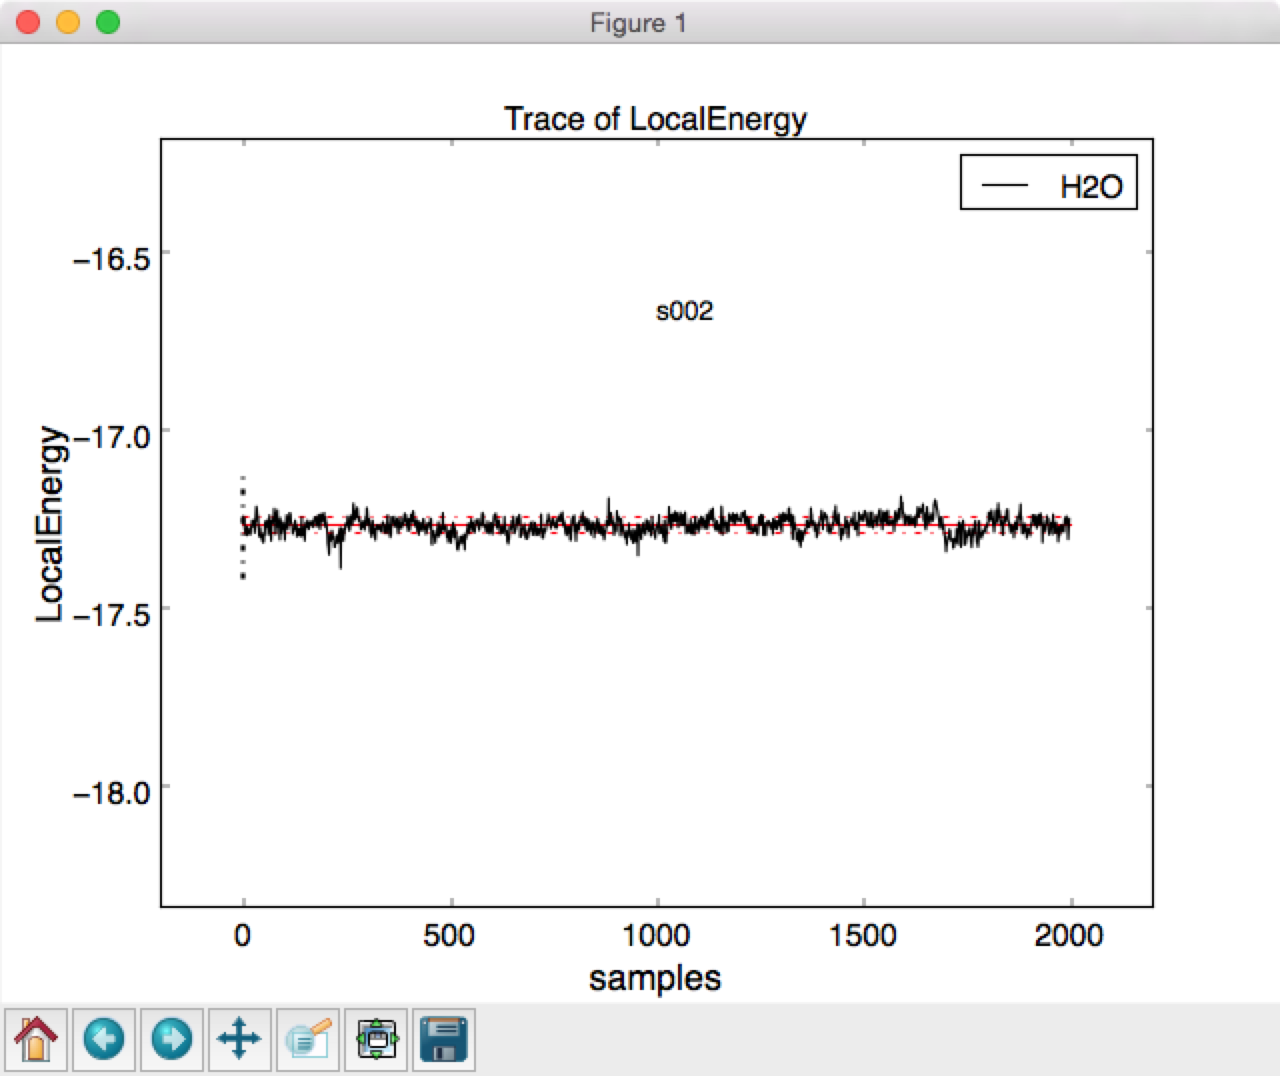
\includegraphics[width=10cm]{./figures/quick_qmca_dmc_trace.png}
  \caption{Trace of walker energies produced by the qmca tool for a simple
    water molecule example.}
  \label{fig:quick_qmca_dmc_trace}
\end{figure}

\section{Authors and History}
\label{sec:history}
QMCPACK was initially written by Jeongnim Kim while in the group of
Professor David Ceperley at the University of Illinois at
Urbana-Champaign, with later contributations being made at Oak Ridge National Laboratory (ORNL). Over the years, many others have contributed, particularly
students and researchers in the groups of Professor David Ceperley
and Professor Richard M. Martin, as well as staff at Lawrence Livermore
National Laboratory, Sandia National Laboratories, Argonne National
Laboratory, and ORNL.

Additional developers, contributors, and advisors include
Anouar Benali,
Mark A. Berrill,  
David M. Ceperley, 
Simone Chiesa,
Raymond C. III Clay,
Bryan Clark,
Kris T. Delaney,
Kenneth P. Esler,
Paul R. C. Kent,
Jaron T. Krogel,
Ying Wai Li,
Ye Luo,
Jeremy McMinis,
Miguel A. Morales,
William D. Parker,
Nichols A. Romero,
Luke Shulenburger,
Norman M. Tubman,
and Jordan E. Vincent.

If you should be added to this list, please let us know.

Development of QMCPACK has been supported financially by
several grants, including the following:

\begin{itemize}
\item ``Network for ab initio many-body methods: development, education
  and training'' supported through the Predictive
  Theory and Modeling for Materials and Chemical Science program by
  the U.S. Department of Energy Office of Science, Basic Energy
  Sciences
\item ``QMC Endstation,'' supported by Accelerating Delivery of Petascale
  Computing Environment at the DOE Leadership Computing Facility at
  ORNL
\item PetaApps, supported by the US National Science
  Foundation
\item Materials Computation Center (MCC), supported by the
  US National Science Foundation
\end{itemize}


\section{Support and Contacting the Developers}
\label{sec:support}

Questions about installing, applying, or extending QMCPACK can be
posted on the QMCPACK Google group at
\url{https://groups.google.com/forum/#!forum/qmcpack}. You may also
email any of the developers, but we recommend checking the group
first. Particular attention is given to any problem reports.

\section{Performance}
\label{sec:performance}

QMCPACK implements modern Monte Carlo (MC) algorithms, is highly parallel,
and is written using very efficient code for high per-CPU or on-node performance. In particular, the code is highly vectorizable,
giving high performance on modern central processing units (CPUs) and GPUs. We believe QMCPACK
delivers performance either comparable to or better than other QMC
codes when similar calculations are run, particularly for the most
common QMC methods and for large systems. If you find a calculation where this is not the
case, or you simply find performance slower than expected, please post on the Google
group or contact one of the developers. These reports are valuable. If your calculation is
sufficiently mainstream we will optimize QMCPACK to improve
the performance.

\section{Open source license}
\label{sec:license}

QMCPACK is distributed under the University of Illinois at
Urbana-Champaign/National Center for Supercomputing Applications (UIUC/NCSA) Open
Source License. 

\begin{verbatim}
		  University of Illinois/NCSA Open Source License

Copyright (c) 2003, University of Illinois Board of Trustees.
All rights reserved.

Developed by:   
  Jeongnim Kim
  Condensed Matter Physics,
  National Center for Supercomputing Applications, University of Illinois
  Materials computation Center, University of Illinois
  http://www.mcc.uiuc.edu/qmc/

Permission is hereby granted, free of charge, to any person obtaining a
copy of this software and associated documentation files (the
``Software''), to deal with the Software without restriction, including
without limitation the rights to use, copy, modify, merge, publish,
distribute, sublicense, and/or sell copies of the Software, and to
permit persons to whom the Software is furnished to do so, subject to
the following conditions:

        * Redistributions of source code must retain the above copyright 
          notice, this list of conditions and the following disclaimers.
        * Redistributions in binary form must reproduce the above copyright 
          notice, this list of conditions and the following disclaimers in 
          the documentation and/or other materials provided with the 
          distribution.
        * Neither the names of the NCSA, the MCC, the University of Illinois, 
          nor the names of its contributors may be used to endorse or promote 
          products derived from this Software without specific prior written 
          permission.

THE SOFTWARE IS PROVIDED "AS IS", WITHOUT WARRANTY OF ANY KIND, EXPRESS
OR IMPLIED, INCLUDING BUT NOT LIMITED TO THE WARRANTIES OF MERCHANTABILITY, 
FITNESS FOR A PARTICULAR PURPOSE AND NONINFRINGEMENT. IN NO EVENT SHALL 
THE CONTRIBUTORS OR COPYRIGHT HOLDERS BE LIABLE FOR ANY CLAIM, DAMAGES OR 
OTHER LIABILITY, WHETHER IN AN ACTION OF CONTRACT, TORT OR OTHERWISE, 
ARISING FROM, OUT OF OR IN CONNECTION WITH THE SOFTWARE OR THE USE OR 
OTHER DEALINGS WITH THE SOFTWARE.
\end{verbatim}

Copyright is generally believed to remain with the authors of the
individual sections of code. See the various notations in the source code as
well as the code history.

\section{Contributing to QMCPACK}
\label{sec:contributing}

QMCPACK is fully open source, and we welcome contributions. If you are
planning a development, early discussions are encouraged. Please
post on the QMCPACK Google group or contact the developers. We can tell you whether anyone else is working on a similar feature or whether
any related work has been done in the past.  Credit for your
contribution can be obtained, for example, through citation of a paper or by
becoming one of the authors on the next version of the standard
QMCPACK reference citation.

A guide to developing for QMCPACK, including instructions on how to
work with GitHub and make pull requests (contributions) to the main
source are listed on the QMCPACK GitHub wiki:
\url{https://github.com/QMCPACK/qmcpack/wiki}.

Contributions are made under the same license as QMCPACK, the
UIUC/NCSA open source license. If this is problematic, please discuss
with a developer.

Please note the following guidelines for contributions:
\begin{itemize}
\item Additions should be fully synchronized with the latest release
  version and ideally the latest develop branch on github. Merging of code
  developed on older versions is error prone.
\item Code should be cleanly formatted, commented, portable, and accessible to
  other programmers. That is, if you need to use any clever tricks, add a comment
  to note this, why the trick is needed, how it works, etc. Although we like
  high performance, ease of maintenance and accessibility are also
  considerations.
\item Comment your code. You are not only writing it for the compiler
  for also for other humans! (We know this is a repeat of the previous
  point, but it is important enough to repeat.)
\item Write a brief description of the method, algorithms, and inputs and outputs
  suitable for inclusion in this manual.
\item Develop some short tests that exercise the
  functionality that can be used for validation and for examples. We
  can help with this and their integration into the test system.
\end{itemize}

\section{QMCPACK Roadmap}
\label{sec:roadmap}

A general outline of the QMCPACK roadmap is given in Sections 1.7.1 and 1.7.2 . Suggestions
for improvements are welcome, particularly those that would facilitate new
scientific applications. For example, if an interface to a particular
quantum chemical or density functional code would help, this would be
given strong consideration.

\subsection{Code}

We will continue to improve the accessibility and usability of
QMCPACK through combinations of more convenient input parameters, improved
workflow, integration with more quantum chemical and density
functional codes, and a wider range of examples.

In terms of methodological development, we expect to significantly
increase the range of QMC algorithms in QMCPACK in the near future.

Computationally, we are porting QMCPACK to the next generation of
supercomputer systems. The internal changes required to run efficiently on these
systems are expected to benefit \emph{all} platforms due
to improved vectorization, cache utilization, and memory performance.

\subsection{Documentation}

This manual describes the core features of QMCPACK that are
required for routine research calculations, i.e., the VMC and DMC
methods, how to obtain and optimize trial wavefunctions, and simple
observables. Over time this manual will be expanded to include a
broader introduction to QMC methods and to describe more features of
the code.

Because of its history as a research code, QMCPACK contains a variety of
additional QMC methods, trial wavefunction forms, potentials, etc.,
that, although not critical, might be very useful for specialized
calculations or particular material or chemical systems. These
``secret features'' (every code has these) are not actually secret but
simply lack descriptions, example inputs, and tests. You are
encouraged to browse and read the source code to find them. New
descriptions will be added over time but can also be prioritized and
added on request (e.g., if a specialized Jastrow factor would help or
a historical Jastrow form is needed for benchmarking).



\chapter{Features of QMCPACK}
\label{chap:features}
\section{Features in production}
\begin{itemize}
\item Variational Monte Carlo
\item Diffusion Monte Carlo
\item Reptation Monte Carlo
\item Single and multi-determinant Slater Jastrow wavefunctions
\item Wavefunction updates using optimized multi-determinant algorithm of Clark et al.
\item Backflow wavefunctions
\item One, two, and three-body Jastrow factors
\item Excited state calculations via flexible occupancy assignment of Slater determinants
\item All electron and non-local pseudopotential calculations
\item Casula T-moves for variational evaluation of non-local pseudopotentials
\item Wavefunction optimization using the ``linear method'' of Umrigar and co-workers, with arbitrary mix of variance and energy in the objective function
\item Gaussian, Slater, plane-wave and real-space spline basis sets for orbitals
\item Interface and conversion utilities for plane-wave wavefunctions from Quantum Espresso (PWSCF)
\item Interface and conversion utilities for Gaussian-basis wavefunctions from GAMESS
\item Easy extension and interfacing to other electronic structure codes via standardized XML and HDF5 inputs
\item MPI parallelism
\item Fully threaded using OpenMP
\item GPU (CUDA) implementation (limited functionality)
\item HDF5 input/output for large data
\item Nexus: advanced workflow tool to automate all aspects of QMC calculation from initial DFT calculations through to final analysis
\item Analysis tools for minimal environments (perl only) through to python-based with graphs produced via matplotlib.
\end{itemize}

\subsection{Supported GPU features}

\begin{itemize}

  \item VMC, wavefunction optimization, DMC are supported
  \item Periodic and open boundary conditions are fully supported. Mixed boundary conditions are not yet supported.
  \item Wavefunctions:
    \begin{enumerate}
        \item Single Slater determinants with 3D B-spline orbitals. Twist-averaged boundary conditions and complex wavefunctions are fully supported. Gaussian type orbitals are not supported yet.
        \item Mixed basis representation in which orbitals are represented as 1D splines times spherical harmonics in spherical regions (muffin tins) around atoms, and 3D B-splines in the interstitial region.
        \item One-body and two-body Jastrows represented as 1D B-splines are supported.
    \end{enumerate}
  \item Semilocal (nonlocal and local) pseudopotentials, Coulomb interaction (electron-electron, electron-ion) and Model periodic Coulomb (MPC) interaction are all supported.
\end{itemize}

\section{Features in beta test}
This section describes developmental features in QMCPACK that might be ready for production, but require additional testing, features or documentation to be ready for general use. We describe them here because they offer significant benefits and are well tested in specific cases.

\subsection{CPU SoA optimization}
SoA stands for Structure-of-Arrays which is a data layout facilitating vectorization on modern CPUs with wide SIMD units. The SoA optimization \cite{IPCC_SC17} for CPUs significantly boost the performance of QMCPACK. Meanwhile, the memory footprint is dramatically reduced by introducing compute-on-the-fly algorithms. To get all the benefit, compilers support OpenMP 4.0 SIMD are recommended. \textbf{Users should check what we specifically test on cdash/ctest and to make specific requests to expand the functionality that they need.}

SoA code path currently supports:
\begin{itemize}
  \item VMC, wavefunction optimization, DMC, RMC are all supported
  \item Periodic, open and mixed boundary conditions are fully supported.
  \item Wavefunctions:
    \begin{enumerate}
      \item Single and multiple Slater determinants with 3D B-spline orbitals. Twist-averaged boundary conditions and complex wavefunctions are fully supported. Gaussian type orbitals are not supported yet.
      \item Hybrid representation, to be ready soon.
      \item One-body and two-body Jastrows represented as 1D B-splines and three-body Jastrow represented as polynomials are supported.
    \end{enumerate}
  \item Semilocal (nonlocal and local) pseudopotentials, Coulomb interaction (electron-electron, electron-ion) and MPC are all supported.
\end{itemize}

\chapter{Obtaining, installing and validating QMCPACK}
\label{chap:obtaininginstalling}

This chapter describes how to obtain, build and validate QMCPACK. This process is designed to be as simple as
possible and should be no harder than building a modern plane-wave density
functional theory code such as Quantum ESPRESSO, QBox, or
VASP. Parallel builds enable a complete
compilation in under 2 minutes on a fast multicore system. If you
are unfamiliar with building codes we suggest working with your system
administrator to install QMCPACK.

\section{Installation steps}
To install QMCPACK, follow the steps listed below. Full details of
each step are given in the referenced sections.
\begin{enumerate}
\item Download the source code, Sections \ref{sec:obrelease} or \ref{sec:obdevelopment}.
\item Verify that you have the required compilers, libraries and tools
  installed, Section \ref{sec:prerequisites}.
\item Run the cmake configure step and build with make, Section
  \ref{sec:cmake} and \ref{sec:cmakequick}. Some examples for common
  systems are given in Section \ref{sec:installexamples}.
\item Run the tests to verify QMCPACK, Section \ref{sec:testing}.
\item Build the ppconvert utility in QMCPACK, Section \ref{sec:buildppconvert}.
\item Download and patch Quantum ESPRESSO. This patch adds the
  pw2qmcpack utility, Section \ref{sec:buildqe}.
\end{enumerate}

Hints for high performance are in Section \ref{sec:buildperformance}. Troubleshooting suggestions are in Section \ref{sec:troubleshoot}.

Note that there are two different QMCPACK executables that can be
produced: the general one, which is the default, and the ``complex''
version which support periodic calculations at arbitrary twist angles and
k-points. This second version is enabled via a cmake configuration
parameter, see Section \ref{sec:cmakeoptions}. The general version
only supports wavefunctions that can be made real. If you run a
calculation that needs the complex version, QMCPACK will stop and inform you.

\section{Obtaining the latest release version}
\label{sec:obrelease}
Major releases of QMCPACK are distributed from
\url{http://www.qmcpack.org}. These releases undergo the most testing. Unless there are
specific reasons we encourage all production calculations to use the
latest release versions.

Releases are usually compressed tar files indicating the version
number, date, and often the source code revision control number
corresponding to the release.

\begin{itemize}
\item Download the latest QMCPACK distribution from \url{http://www.qmcpack.org}.
\item Untar the archive, e.g., \texttt{tar xvf qmcpack\_v1.3.tar.gz}
\end{itemize}

Releases can also be obtained from the 'master' branch of the QMCPACK
git repository, similar to obtaining the development version (Sec. \ref{sec:obdevelopment}).

\section{Obtaining the latest development version}
\label{sec:obdevelopment}
The most recent development version of QMCPACK can be obtained anonymously via
\begin{verbatim}
git clone https://github.com/QMCPACK/qmcpack.git
\end{verbatim}
Once checked-out,
updates can be made via the standard \texttt{git pull}.

The 'develop' branch of the git repository contains the day-to-day development source
with the latest updates, bugfixes etc. This may be useful
for updates to the build system to support new machines, for support
of the latest versions of Quantum ESPRESSO, or for updates to the
documentation.  Note that the development version may not be fully
consistent with the online documentation.  We attempt to keep
the development version fully working. However, please be sure to run the tests and
compare with previous release versions before using for any serious
calculations. We try to keep bugs out, but occasionally they crawl
in! Reports of any breakages are appreciated.

\section{Prerequisites}
\label{sec:prerequisites}
The following are required to build QMCPACK. For workstations, these are available via the standard
package manager. On shared supercomputers this software is usually
installed by default and is often
access via a modules environment - check your system
documentation.

\textbf{Use of the latest versions of all compilers and libraries is
strongly encouraged}, but not absolutely essential. Generally newer versions are faster - see
Section \ref{sec:buildperformance} for performance suggestions.

\begin{itemize}
\item C/C++ compilers such as GCC, Intel, IBM XLC. LLVM-based compilers
  are supported only on a preliminary basis.
\item MPI library such at OpenMPI \url{http://open-mpi.org}
\item BLAS/LAPACK, numerical and linear algebra libraries. Use
  platform-optimized libraries where available, such as Intel MKL.
  ATLAS or other optimized open-source libraries may also be used
  \url{http://math-atlas.sourceforge.net}
\item CMake, build utility, \url{http://www.cmake.org}
\item Libxml2, XML parser, \url{http://xmlsoft.org}
\item HDF5, portable I/O library, \url{http://www.hdfgroup.org/HDF5/}
\item BOOST, peer-reviewed portable C++ source libraries, \url{http://www.boost.org}
\item FFTW, FFT library, \url{http://www.fftw.org/}
\end{itemize}

To build the GPU accelerated version of QMCPACK an installation of
NVIDIA CUDA development tools is required. Ensure that this is
compatible with the C and C++ compiler versions you plan to
use. Supported versions are included in the NVIDIA release notes.

Many of the utilities provided with QMCPACK use python (v2). The numpy
and matplotlib libraries are required for full functionality.

Note that the standalone einspline library used by previous versions of QMCPACK
is no longer required. A more optimized version is included
inside. The standalone version should \emph{not} be on any standard
search paths because conflicts between the old and new include files
can result.

\section{Building with CMake}
\label{sec:cmake}
The build system for QMCPACK is based on CMake.  It will autoconfigure
based on the detected compilers and libraries. The most recent
version of CMake has the best detection for the greatest variety of
systems - at the time of writing this means CMake 3.4.3. The much
older CMake 2.8 is known to work, but might not work optimally on your system.

Previously QMCPACK made extensive use of toolchains, but the build system
has since been updated to eliminate the use of toolchain files for
most cases.  The build system is verified to work with GNU, Intel, and IBM XLC
compilers.  Specific compile options can be specified either through
specific environmental or CMake variables.  When the libraries are
installed in standard locations, e.g., /usr, /usr/local, there is no
need to set environmental or cmake variables for the packages.

\subsection{Quick build instructions (try first)}
\label{sec:cmakequick}

If you are feeling lucky and are on a standard UNIX-like system such
as a Linux workstation, the following might quickly give a
working QMCPACK:

The safest quick build option is to specify the C and C++ compilers
through their MPI wrappers. Here we use Intel MPI and Intel
compilers. Move to the build directory, run cmake and make
\begin{verbatim}
cd build
cmake -DCMAKE_C_COMPILER=mpiicc -DCMAKE_CXX_COMPILER=mpiicpc ..
make -j 8
\end{verbatim}
You can increase the ``8'' to the number of cores on your system for
faster builds. Substitute mpicc and mpicxx or other wrapped compiler names to suit
  your system. e.g. With OpenMPI use
\begin{verbatim}
cd build
cmake -DCMAKE_C_COMPILER=mpicc -DCMAKE_CXX_COMPILER=mpicxx ..
make -j 8
\end{verbatim}

If you are feeling particularly lucky, you can skip the compiler specification:
\begin{verbatim}
cd build
cmake ..
make -j 8
\end{verbatim}

The complexities of modern computer hardware and software systems are
such that you should check that the autoconfiguration system has made
good choices and picked optimized libraries and compiler settings
before doing significant production. i.e. Check the details below. We
give examples for a number of common systems in Section \ref{sec:installexamples}.

\subsection{Environment variables}
\label{sec:envvar}
A number of environmental variables affect the build.  In particular
they can control the default paths for libraries, the default
compilers, etc.  The list of environmental variables is given below:
\begin{verbatim}
CXX              C++ compiler
CC               C Compiler
MKL_HOME         Path for MKL
LIBXML2_HOME     Path for libxml2
HDF5_ROOT        Path for HDF5
BOOST_ROOT       Path for Boost
FFTW_HOME        Path for FFTW
\end{verbatim}

\subsection{Configuration options}
\label{sec:cmakeoptions}
In addition to reading the environmental variables, CMake provides a
number of optional variables that can be set to control the build and
configure steps.  When passed to CMake, these variables will take
precedent over the environmental and default variables.  To set them
add -D FLAG=VALUE to the configure line between the cmake command and
the path to the source directory.

\begin{itemize}
\item  Key QMCPACK build options
\begin{verbatim}
QMC_CUDA            Enable CUDA and GPU acceleration (1:yes, 0:no)
QMC_COMPLEX         Build the complex (general twist/k-point) version (1:yes, 0:no)
QMC_MIXED_PRECISION Build the mixed precision (mixing double/float) version
                    (1:yes (GPU default), 0:no (CPU default)).
                    The CPU support is experimental.
                    Use float and double for base and full precision.
                    The GPU support is quite mature.
                    Use always double for host side base and full precision
                    and use float and double for CUDA base and full precision.
\end{verbatim}
  \item General build options
\begin{verbatim}
CMAKE_BUILD_TYPE   A variable which controls the type of build
                   (defaults to Release). Possible values are:
                   None (Do not set debug/optmize flags, use
                   CMAKE_C_FLAGS or CMAKE_CXX_FLAGS)
                   Debug (create a debug build)
                   Release (create a release/optimized build)
                   RelWithDebInfo (create a release/optimized build with debug info)
                   MinSizeRel (create an executable optimized for size)
CMAKE_C_COMPILER   Set the C compiler
CMAKE_CXX_COMPILER Set the C++ compiler
CMAKE_C_FLAGS      Set the C flags.  Note: to prevent default
                   debug/release flags from being used, set the CMAKE_BUILD_TYPE=None
                   Also supported: CMAKE_C_FLAGS_DEBUG,
                   CMAKE_C_FLAGS_RELEASE, and CMAKE_C_FLAGS_RELWITHDEBINFO
CMAKE_CXX_FLAGS    Set the C++ flags.  Note: to prevent default
                   debug/release flags from being used, set the CMAKE_BUILD_TYPE=None
                   Also supported: CMAKE_CXX_FLAGS_DEBUG,
                   CMAKE_CXX_FLAGS_RELEASE, and CMAKE_CXX_FLAGS_RELWITHDEBINFO
\end{verbatim}
\item Additional QMCPACK build options
\begin{verbatim}
QMC_INCLUDE         Add extra include paths
QMC_EXTRA_LIBS      Add extra link libraries
QMC_BUILD_STATIC    Add -static flags to build
QMC_DATA            Specify data directory for QMCPACK (currently
                    unused, but likely to be used for future performance tests)
\end{verbatim}
\item libxml related
\begin{verbatim}
Libxml2_INCLUDE_DIRS  Specify include directories for libxml2
Libxml2_LIBRARY_DIRS  Specify library directories for libxml2
\end{verbatim}
 \item FFTW related
\begin{verbatim}
FFTW_INCLUDE_DIRS   Specify include directories for FFTW
FFTW_LIBRARY_DIRS   Specify library directories for FFTW
\end{verbatim}
 \item CTest related
\begin{verbatim}
MPIEXEC   Specify the mpi wrapper, e.g. srun, aprun, mpirun, etc.
MPIEXEC_NUMPROC_FLAG   Specify the number of mpi processes flag, e.g. "-n", "-np", etc.

\end{verbatim}
\end{itemize}

\subsection{Configure and build using cmake and make}
To configure and build QMPACK, move to build directory, run cmake and make
\begin{verbatim}
cd build
cmake ..
make -j 8
\end{verbatim}

As you will have gathered, cmake encourages ``out of source'' builds,
where all the files for a specific build configuration reside in their
own directory separate from the source files. This allows multiple
builds to be created from the same source files which is very useful
where the filesystem is shared between different systems. You can also
build versions with different settings (e.g. QMC\_COMPLEX) and
different compiler settings. The build directory does not have to be
called build - use something descriptive such as build\_machinename or
build\_complex. The ``..'' in the cmake line refers to the directory
containing CMakeLists.txt. Update the ``..'' for other build
directory locations.

\subsection{Example configure and build}
\begin{itemize}
\item Set the environments (the examples below assume bash, Intel compilers and MKL library)
\begin{verbatim}
export CXX=icpc
export CC=icc
export MKL_HOME=/usr/local/intel/mkl/10.0.3.020
export LIBXML2_HOME=/usr/local
export HDF5_ROOT=/usr/local
export BOOST_ROOT=/usr/local/boost
export FFTW_HOME=/usr/local/fftw
\end{verbatim}

\item Move to build directory, run cmake and make
\begin{verbatim}
cd build
cmake -D CMAKE_BUILD_TYPE=Release ..
make -j 8
\end{verbatim}
\end{itemize}

\subsection{Build scripts}
It is recommended to create a helper script that contains the
configure line for CMake.  This is particularly useful when avoiding
environmental variables, packages are installed in custom locations,
or if the configure line is long or complex.  In this case it is also
recommended to add "rm -rf CMake*" before the configure line to remove
existing CMake configure files to ensure a fresh configure each time
that the script is called. Deleting all the files in the build
directory is also acceptable. If you do so we recommend to add some sanity
checks in case the script is run from the wrong directory, e.g.,
checking for the existence of some QMCPACK files.

Some build script examples for different systems are given in the
config directory. For example, on Cray systems these scripts might
load the appropriate modules to set the appropriate programming
environment, specific library versions etc.

An example script build.sh is given below. It is much more complex
than usually needed for comprehensiveness:

\begin{verbatim}
export CXX=mpic++
export CC=mpicc
export ACML_HOME=/opt/acml-5.3.1/gfortran64
export HDF5_ROOT=/opt/hdf5
export BOOST_ROOT=/opt/boost

rm -rf CMake*

cmake                                                \
  -D CMAKE_BUILD_TYPE=Debug                         \
  -D Libxml2_INCLUDE_DIRS=/usr/include/libxml2      \
  -D Libxml2_LIBRARY_DIRS=/usr/lib/x86_64-linux-gnu \
  -D FFTW_INCLUDE_DIRS=/usr/include                 \
  -D FFTW_LIBRARY_DIRS=/usr/lib/x86_64-linux-gnu    \
  -D QMC_EXTRA_LIBS="-ldl ${ACML_HOME}/lib/libacml.a -lgfortran" \
  -D QMC_DATA=/projects/QMCPACK/qmc-data            \
  ..
\end{verbatim}

\subsection{Using vendor optimized numerical libraries, e.g. Intel MKL}
 
Although QMC does not make extensive use of linear algebra, use of
vendor optimized libraries is strongly recommended for highest
performance. BLAS routines are used in the Slater determinant update, the VMC wavefunction optimizer
and to apply orbital coefficients in local basis calculations. Vectorized
math functions are also beneficial, e.g. for the phase factor
computation in solid state calculations. CMake is generally successful
in finding these libraries, but specific combinations can require
additional hints, as described below:

\subsubsection{Using Intel MKL with non-Intel compilers}

To use Intel MKL with, e.g. an MPICH wrapped gcc:
\begin{verbatim}
cmake \
 -DCMAKE_C_COMPILER=mpicc -DCMAKE_CXX_COMPILER=mpicxx \
 -DBLA_VENDOR=Intel10_64lp_seq -DCMAKE_PREFIX_PATH=$MKLROOT/lib \
 ..
\end{verbatim}

MKLROOT is the directory containing the MKL binary, examples, and lib
directories (etc.) and is often /opt/intel/mkl 


\section{Installation instructions for common workstations and
  supercomputers}
\label{sec:installexamples}

This section describes how to build QMCPACK on various common systems
including multiple Linux distributions, Apple OS X, and various
supercomputers. The examples should serve as good starting points for
building QMCPACK on similar machines. For example, the software
environment on modern Crays is very consistent. Note that updates to
operating systems and system software may require small modifications
to these recipes. See Section \ref{sec:buildperformance} for key
points to check to obtain highest performance and
Section \ref{sec:troubleshoot} for troubleshooting hints.

\subsection{Installing on Ubuntu Linux or other apt-get based distributions}
\label{sec:buildubuntu}

The following is designed to obtain a working QMCPACK build on e.g. a
student laptop, starting from a basic Linux installation with none of
the developer tools installed. Fortunately, all the required packages
are available in the default repositories making for a quick
installation. Note that for convenience we use a generic BLAS. For
production a platform optimized BLAS should be used.

\begin{verbatim}
apt-get cmake g++ openmpi-bin libopenmpi-dev libboost-dev
apt-get libatlas-base-dev liblapack-dev libhdf5-dev libxml2-dev fftw3-dev
export CXX=mpiCC
cd build
cmake ..
make -j 8
ls -l bin/qmcpack
\end{verbatim}

For qmca and other tools to function, we install some python libraries:
\begin{verbatim}
sudo apt-get install python-numpy python-matplotlib
\end{verbatim}

\subsection{Installing on CentOS Linux or other yum based distributions}

The following is designed to obtain a working QMCPACK build on e.g. a
student laptop, starting from a basic Linux installation with none of
the developer tools installed. CentOS 7 (Red Hat compatible) is using
gcc 4.8.2. The installation is only complicated by the need to install
another repository to obtain HDF5 packages which are not available by
default. Note that for convenience we use a generic BLAS. For
production a platform optimized BLAS should be used.

\begin{verbatim}
sudo yum install make cmake gcc gcc-c++ openmpi openmpi-devel fftw fftw-devel \
                  boost boost-devel libxml2 libxml2-devel
sudo yum install blas-devel lapack-devel atlas-devel
module load mpi
\end{verbatim}

To setup repoforge as a source for the HDF5 package, go to
\url{http://repoforge.org/use} . Install the appropriate up to date
release package for your OS. By default the CentOS Firefox will offer
to run the installer. The CentOS 6.5 settings were still usable for HDF5 on
CentOS 7 in 2016, but use CentOS 7 versions when they become
available.

\begin{verbatim}
sudo yum install hdf5 hdf5-devel
\end{verbatim}

To build QMCPACK
\begin{verbatim}
module load mpi/openmpi-x86_64
which mpirun
# Sanity check; should print something like   /usr/lib64/openmpi/bin/mpirun
export CXX=mpiCC
cd build
cmake ..
make -j 8
ls -l bin/qmcpack
\end{verbatim}

\subsection{Installing on Mac OS X using Macports}
These instructions assume a fresh installation of macports
and use the gcc 6.1 compiler. Older versions are fine, but it is vital to ensure
matching compilers and libraries are used for all
packages and to force use of what is installed in /opt/local.  Performance should be very reasonable.
Note that we utilize the Apple provided Accelerate framework for
optimized BLAS.

Follow the Macports install instructions \url{https://www.macports.org/}

\begin{itemize}
\item Install Xcode and the Xcode Command Line Tools
\item Agree to Xcode license in Terminal: sudo xcodebuild -license
\item Install MacPorts for your version of OS X
\end{itemize}


Install the required tools:

\begin{verbatim}
sudo port install gcc6
sudo port select gcc mp-gcc6
sudo port install openmpi-devel-gcc6
sudo port select --set mpi openmpi-devel-gcc61-fortran

sudo port install fftw-3 +gcc6
sudo port install libxml2
sudo port install cmake
sudo post install boost +gcc6
sudo port install hdf5 +gcc6

sudo port select --set python python27
sudo port install py27-numpy +gcc6
sudo port install py27-matplotlib  #For graphical plots with qmca
\end{verbatim}

QMCPACK build:
\begin{verbatim}
cd build
cmake -DCMAKE_C_COMPILER=mpicc -DCMAKE_CXX_COMPILER=mpiCXX ..
make -j 6 # Adjust for available core count
ls -l bin/qmcpack
\end{verbatim}

Cmake should pickup the versions of HDF5, libxml (etc.) installed in
/opt/local by macports. If you have other copies of these libraries
installed and wish to force use of a specific version, use the
environment variables detailed in Sec. \ref{sec:envvar}.

This recipe was verified on 1 July 2016 on a Mac running OS X 10.11.5
``El Capitain''.

\subsection{Installing on Mac OS X using Homebrew (brew)}
Homebrew is a package manager for OS X that provides a convenient
route to install all the QMCPACK dependencies. The
following recipe will install the latest available versions of each
package. This was successfully tested under OS X 10.11 ``El
Capitain'' in February 2016. Note that it is necessary to build the MPI software from
source to use the brew-provided gcc instead of Apple CLANG.

\begin{enumerate}
\item Install Homebrew from \url{http://brew.sh/}
\begin{verbatim}
/usr/bin/ruby -e "$(curl -fsSL
    https://raw.githubusercontent.com/Homebrew/install/master/install)"
\end{verbatim}

\item Install the prerequisites
\begin{verbatim}
brew install gcc # Builds full gcc 5 from scratch, will take 30 minutes
export HOMEBREW_CXX=g++-5
export HOMEBREW_CC=gcc-5
brew install mpich2 --build-from-source
# Build from source required to use homebrew compiled compilers as
# opposed to Apple CLANG. Check "mpicc -v" indicates Homebrew gcc 5.x.x
brew install cmake
brew install fftw
brew install boost
brew install homebrew/science/hdf5
#Note: Libxml2 is not required via brew since OS X already includes it.
\end{verbatim}
\item Configure and build QMCPACK
\begin{verbatim}
cmake -DCMAKE_C_COMPILER=/usr/local/bin/mpicc \
      -DCMAKE_CXX_COMPILER=/usr/local/bin/mpicxx ..
make -j 12
\end{verbatim}
\item Run the short tests. When mpich is used for the first time, OS
  X will request approval of the network connection.
\begin{verbatim}
ctest -R short
\end{verbatim}
\end{enumerate}

\subsection{Installing on ANL ALCF Mira/Cetus IBM Blue Gene/Q}
\label{sec:buildbgq}
Mira/Cetus is a Blue Gene/Q supercomputer at Argonne National Laboratory's Argonne Leadership Computing Facility (ANL ALCF). Mira has 49152 compute nodes and each node has a 16-core PowerPC A2 processor with 16 GB DDR3 memory. Due to the fact that the login nodes and the compute nodes have different processors with distinct instruction sets, cross-compiling is required on this platform. See details about using Blue Gene/Q at \url{http://www.alcf.anl.gov/user-guides/compiling-linking}. On Mira, compilers are loaded via softenv and users need to add +mpiwrapper-xl and +cmake in \$HOME/.soft. In order to build QMCPACK, a toolchain file is provided for setting up CMake and the cmake command should be executed twice.

\begin{verbatim}
cd build
cmake -DCMAKE_TOOLCHAIN_FILE=../config/BGQ_Clang++11_ToolChain.cmake ..
cmake -DCMAKE_TOOLCHAIN_FILE=../config/BGQ_Clang++11_ToolChain.cmake ..
make -j 16
ls -l bin/qmcpack
\end{verbatim}

In addition, adding a very useful cmake option
-DCMAKE\_VERBOSE\_MAKEFILE=TRUE allows printing all the build commands
during the make step. Alternatively you can use make VERBOSE=1.

\subsection{Installing on ORNL OLCF Titan Cray XK7 (NVIDIA GPU
  accelerated)}
\label{sec:titanbuildgpu}
Titan is a GPU accelerated supercomputer at Oak Ridge National
Laboratory's  Oak Ridge Leadership Computing Facility  (ORNL OLCF). Each
compute node has a 16 core AMD 2.2GHz Opteron 6274 (Interlagos) and an
NVIDIA Kepler accelerator. The standard Cray software environment is
available, with libraries accessed via modules. The only extra
settings required to build the GPU version are the cudatoolkit module
and specifying -DQMC\_CUDA=1 on the cmake configure line.

Note that on Crays the compiler wrappers ``CC'' and ``cc'' are
used. The build system checks for these and does not (should not) use
the compilers directly.

\begin{verbatim}
module swap PrgEnv-pgi PrgEnv-gnu # Use gnu compilers
module load cudatoolkit           # CUDA for GPU build
module load cray-hdf5
module load cmake
module load fftw
export FFTW_HOME=$FFTW_DIR/..
module load boost
mkdir build_titan_gpu
cd build_titan_gpu
cmake -DQMC_CUDA=1 ..             # Must enable CUDA capabilities
make -j 8
ls -l bin/qmcpack
\end{verbatim}

\subsection{Installing on ORNL OLCF Titan Cray XK7 (CPU version)}
As noted in Section\ref{sec:titanbuildgpu} for the GPU, building on
Crays requires only loading the appropriate library modules.

\begin{verbatim}
module swap PrgEnv-pgi PrgEnv-gnu # Use gnu compilers
module unload cudatoolkit         # No CUDA for CPU build
module load cray-hdf5
module load cmake
module load fftw
export FFTW_HOME=$FFTW_DIR/..
module load boost
mkdir build_titan_cpu
cd build_titan_cpu
cmake ..
make -j 8
ls -l bin/qmcpack
\end{verbatim}

\subsection{Installing on ORNL OLCF Eos Cray XC30}
Eos is a Cray XC30 with 16 core Intel Xeon E5-2670 processors connected
by the Aries interconnect. The build process is identical to Titan,
except that we use the default Intel programming environment. This is
usually preferred to GNU.
\begin{verbatim}
module load cray-hdf5
module load cmake
module load fftw
export FFTW_HOME=$FFTW_DIR/..
module load boost
mkdir build_eos
cd build_eos
cmake ..
make -j 8
ls -l bin/qmcpack
\end{verbatim}

\subsection{Installing on ORNL OLCF SummitDev}
SummitDev is the development cluster for the next GPU accelerated
supercomputer Summit at Oak Ridge National Laboratory's
Leadership Computing Facility  (ORNL OLCF). It has IBM Power8 CPUs and NVIDIA Pascal GPUs.

\subsubsection{Building QMCPACK}
Please note that these build instructions are preliminary as the
software environment is subject to change. QMCPACK can be build with the following commands:
\begin{verbatim}
module load xl
module load essl
module load netlib-lapack
module load hdf5/1.8.18
module load fftw
export FFTW_HOME=$OLCF_FFTW_ROOT
module load python
module load cmake
module load boost
module load cuda
mkdir build_summitdev
cd build_summitdev
cmake -DCMAKE_C_COMPILER="mpixlc" \
      -DCMAKE_CXX_COMPILER="mpixlC" \
      -DBUILD_LMYENGINE_INTERFACE=0 \
      -DQMC_CUDA=1 \
      -DCUDA_ARCH="sm_60" \
      ..
make -j 8
ls -l bin/qmcpack
\end{verbatim}

\subsection{Installing on NERSC Edison Cray XC30}

Edison is a Cray XC30 with dual 12-core Intel "Ivy Bridge" nodes
installed at NERSC. The build settings are identical to eos.

\begin{verbatim}
module load cray-hdf5
module load cmake
module load fftw
export FFTW_HOME=$FFTW_DIR/..
module load boost
mkdir build_edison
cd build_edison
cmake ..
make -j 8
ls -l bin/qmcpack
\end{verbatim}
When the above was tested on 1 February 2016, the following module and
software versions were present:
\begin{verbatim}
qmcpack@edison04:trunk> module list
Currently Loaded Modulefiles:
  1) modules/3.2.10.3                        16) alps/5.2.3-2.0502.9295.14.14.ari
  2) nsg/1.2.0                               17) rca/1.0.0-2.0502.57212.2.56.ari
  3) eswrap/1.1.0-1.020200.1130.0            18) atp/1.8.3
  4) switch/1.0-1.0502.57058.1.58.ari        19) PrgEnv-intel/5.2.56
  5) craype-network-aries                    20) craype-ivybridge
  6) craype/2.5.0                            21) cray-shmem/7.3.0
  7) intel/15.0.1.133                        22) cray-mpich/7.3.0
  8) cray-libsci/13.3.0                      23) slurm/edison
  9) udreg/2.3.2-1.0502.9889.2.20.ari        24) altd/2.0
 10) ugni/6.0-1.0502.10245.9.9.ari           25) darshan/2.3.0
 11) pmi/5.0.10-1.0000.11050.0.0.ari         26) subversion/1.7.9
 12) dmapp/7.0.1-1.0502.10246.8.47.ari       27) cray-hdf5/1.8.14
 13) gni-headers/4.0-1.0502.10317.9.2.ari    28) cmake/2.8.11.2
 14) xpmem/0.1-2.0502.57015.1.15.ari         29) fftw/3.3.4.6
 15) dvs/2.5_0.9.0-1.0502.1958.2.55.ari      30) boost/1.54
\end{verbatim}

\subsection{Installing on NERSC Cori, Haswell Partition, Cray XC40}
Cori is a Cray XC40 with 16-core Intel "Haswell" nodes
installed at NERSC.

\begin{verbatim}
module unload cray-libsci  
module load boost  
module load cray-hdf5-parallel
module load cmake
mkdir build_cori_hsw
cd build_cori_hsw
cmake ..
make -j 16
ls -l bin/qmcpack
\end{verbatim}

When the above was tested on 29 August 2017, the following module and
software versions were present:

\begin{verbatim}
build_cori_hsw> module list
Currently Loaded Modulefiles:
  1) modules/3.2.10.6                              14) alps/6.4.1-6.0.4.0_7.2__g86d0f3d.ari
  2) nsg/1.2.0                                     15) rca/2.2.11-6.0.4.0_13.2__g84de67a.ari
  3) intel/17.0.2.174                              16) atp/2.1.1
  4) craype-network-aries                          17) PrgEnv-intel/6.0.4
  5) craype/2.5.12                                 18) craype-haswell
  6) udreg/2.3.2-6.0.4.0_12.2__g2f9c3ee.ari        19) cray-shmem/7.6.0
  7) ugni/6.0.14-6.0.4.0_14.1__ge7db4a2.ari        20) cray-mpich/7.6.0
  8) pmi/5.0.12                                    21) altd/2.0
  9) dmapp/7.1.1-6.0.4.0_46.2__gb8abda2.ari        22) darshan/3.1.4
 10) gni-headers/5.0.11-6.0.4.0_7.2__g7136988.ari  23) boost/1.61
 11) xpmem/2.2.2-6.0.4.0_3.1__g43b0535.ari         24) cmake/3.3.2
 12) job/2.2.2-6.0.4.0_8.2__g3c644b5.ari           25) cray-hdf5-parallel/1.10.0.3
 13) dvs/2.7_2.2.31-6.0.4.1_6.1__gb3b87e6
\end{verbatim}

\subsection{Installing on NERSC Cori, Xeon Phi KNL Knight's Landing partition, Cray XC40}
The second phase of NERSC's Cori uses Intel
Xeon Phi Knight's Landing (KNL) nodes. The following build recipe ensures that the code
generation is appropriate for the KNL nodes:

\begin{verbatim}
module swap craype-haswell craype-mic-knl  
module unload cray-libsci  
module load boost  
module load cray-hdf5-parallel
module load cmake
mkdir build_cori_knl
cd build_cori_knl
cmake ..
make -j 16
ls -l bin/qmcpack
\end{verbatim}

When the above was tested on 29 August 2017, the following module and
software versions were present:

\begin{verbatim}
build_cori_knl> module list
Currently Loaded Modulefiles:
  1) modules/3.2.10.6                              10) gni-headers/5.0.11-6.0.4.0_7.2__g7136988.ari  19) cray-shmem/7.6.0
  2) nsg/1.2.0                                     11) xpmem/2.2.2-6.0.4.0_3.1__g43b0535.ari         20) cray-mpich/7.6.0
  3) intel/17.0.2.174                              12) job/2.2.2-6.0.4.0_8.2__g3c644b5.ari           21) altd/2.0
  4) craype-network-aries                          13) dvs/2.7_2.2.31-6.0.4.1_6.1__gb3b87e6          22) darshan/3.1.4
  5) craype/2.5.12                                 14) alps/6.4.1-6.0.4.0_7.2__g86d0f3d.ari          23) boost/1.61
  6) udreg/2.3.2-6.0.4.0_12.2__g2f9c3ee.ari        15) rca/2.2.11-6.0.4.0_13.2__g84de67a.ari         24) cray-hdf5-parallel/1.10.0.3
  7) ugni/6.0.14-6.0.4.0_14.1__ge7db4a2.ari        16) atp/2.1.1                                     25) cmake/3.3.2
  8) pmi/5.0.12                                    17) PrgEnv-intel/6.0.4
  9) dmapp/7.1.1-6.0.4.0_46.2__gb8abda2.ari        18) craype-mic-knl
\end{verbatim}

\subsection{Installing on Windows}
Install the Windows Subsystem for Linux and Bash on Windows.
Open a bash shell and follow the install directions for Ubuntu in Section \ref{sec:buildubuntu}.

\section{Testing and validation of QMCPACK}
\label{sec:testing}
We \textbf{strongly encourage} running the included tests each time
QMCPACK is built. These compare the results from the executable with
known-good mean-field, quantum chemical, and other QMC results.

The tests included with QMCPACK currently mainly test the VMC code with
single determinant wavefunction and simple spline Jastrow
wavefunctions, and for gaussian and periodic spline basis
sets. We check that the known mean
field results are obtained with no Jastrow. When Jastrow functions are
included we test against previous QMC data. The tests are statistical
with a generous 3 $\sigma$ tolerance, however the system sizes are
small, typically $<10$ electrons, so the error bars are typically
small. Limited DMC and optimizer tests included and are scheduled for expansion.

 The ``short'' tests only take a few minutes on a 16
core machine. You can run these tests using the command below in the
build directory:

\begin{verbatim}
ctest -R short   # Run the tests with "short" in their name
\end{verbatim}
The output should be similar to the following:
\begin{verbatim}
Test project build_gcc
      Start  1: short-LiH_dimer_ae-vmc_hf_noj-16-1
 1/44 Test  #1: short-LiH_dimer_ae-vmc_hf_noj-16-1 ..............  Passed   11.20 sec
      Start  2: short-LiH_dimer_ae-vmc_hf_noj-16-1-kinetic
 2/44 Test  #2: short-LiH_dimer_ae-vmc_hf_noj-16-1-kinetic ......  Passed    0.13 sec
..
42/44 Test #42: short-monoO_1x1x1_pp-vmc_sdj-1-16 ...............  Passed   10.02 sec
      Start 43: short-monoO_1x1x1_pp-vmc_sdj-1-16-totenergy
43/44 Test #43: short-monoO_1x1x1_pp-vmc_sdj-1-16-totenergy .....  Passed    0.08 sec
      Start 44: short-monoO_1x1x1_pp-vmc_sdj-1-16-samples
44/44 Test #44: short-monoO_1x1x1_pp-vmc_sdj-1-16-samples .......  Passed    0.08 sec

100% tests passed, 0 tests failed out of 44

Total Test time (real) = 167.14 sec
\end{verbatim}
Note that the number of tests that are run varies between the
standard, complex, and GPU compilations.

The  full set of tests consist of significantly longer versions of the short
tests, as well as tests of the conversion utilities. The runs require
several hours each for improved statistics and a much more
stringent test of the code. To run all the tests simply run ctest in the build
directory:

\begin{verbatim}
ctest            # Run all the tests. This will take several hours.
\end{verbatim}

You can also run verbose tests which direct the QMCPACK
output to the standard output:
\begin{verbatim}
ctest -V -R short   # Verbose short tests
\end{verbatim}

The test system includes specific tests for the complex version of the code.

The data files for the tests are located in the tests directory. The
runs occur in build/tests/system/test\_name. The numerical
comparisons and test definitions are in
tests/system/CMakeLists.txt. If \textit{all} the QMC tests fail it is likely
that the appropriate mpiexec (or aprun, srun) is not being
called or found. If the QMC runs appear to work but all the other
tests fail it is possible that python is not working on your system -
we suggest checking some of the test outputs in build/test/system/test\_name.

Note that because most of these tests are very small, consisting of only a few
electrons, the performance is not representative of larger
calculations. For example, while the calculations might fit in cache,
there will be essentially no vectorization due to the small electron
counts. \textbf{These tests should therefore not be used for any benchmarking or
performance analysis}.

Example runs that can be used for testing performance are described in
Sec. \ref{sec:perftests}

\subsection{Unit tests}

QMCPACK has a set of unit tests.
All of the unit tests can be run with the following command (in the build directory):
\begin{verbatim}
ctest -L unit
\end{verbatim}

The output should look similar to the following:
\begin{verbatim}
Test project qmcpack/build
      Start  1: unit_test_numerics
 1/11 Test  #1: unit_test_numerics ...............   Passed    0.06 sec
      Start  2: unit_test_utilities
 2/11 Test  #2: unit_test_utilities ..............   Passed    0.02 sec
      Start  3: unit_test_einspline
 ...
10/11 Test #10: unit_test_hamiltonian ............   Passed    1.88 sec
      Start 11: unit_test_drivers
11/11 Test #11: unit_test_drivers ................   Passed    0.01 sec

100% tests passed, 0 tests failed out of 11

Label Time Summary:
unit    =   2.20 sec

Total Test time (real) =   2.31 sec
\end{verbatim}

Individual unit test executables can be found in \texttt{build/tests/bin}.
The source for the unit tests is located in the \texttt{tests} directory under each directory in \texttt{src} (e.g. \texttt{src/QMCWavefunctions/tests}).

See Chapter \ref{chap:unit_testing} for more details about unit tests.

\subsection{Integration tests with Quantum Espresso}
\label{sec:integtestqe}
As described in Sec. \ref{sec:buildqe}, it is possible to test entire
workflows of trial wavefunction generation, conversion, and eventual
QMC calculation. A patched QE must be installed so that the
pw2qmcpack converter is available.

By adding \texttt{-D QE\_BIN=your\_QE\_binary\_path} in the cmake command line when building your QMCPACK,
tests named with ``qe-'' prefix will be included in the test set of your build.
You can test the whole pw$\to$pw2qmcpack$\to$qmcpack workflow by
\begin{verbatim}
ctest -R qe
\end{verbatim}
This provides a very solid test of the entire QMC
toolchain for planewave generated wavefunctions.

\subsection{Performance tests}
\label{sec:perftests}
Performance tests representative of real research runs are included in the
tests/performance directory. They can be used for benchmarking, comparing machine
performance, or assessing optimizations. This is in
contrast to the majority of the conventional integration tests where the particle
counts are too small to be representative. Care is still needed to
remove initiallization, I/O, and compute a representative performance
measure.

The ctest integration is sufficient to run the benchmarks and measure
relative performance from version to version of QMCPACK and assess
proposed code changes. Performance tests are prefixed with
``performance''. To obtain highest performance on a particular
platform, you must run the benchmarks in a standalone manner and tune
thread counts, placement, walker count (etc.) This is essential to
fairly compare different machines. Check with the
developers if you are unsure of what is a fair change.

\subsubsection{NiO performance tests}

Follow the instructions in tests/performance/NiO/README to
enable and run the NiO tests.

The NiO tests are for bulk supercells of varying size. The QMC runs consist of short blocks of (i) VMC
without drift (ii) VMC with drift term included (iii) DMC with
constant population. The tests use spline wavefunctions that must be
downloaded as described in the README due to their large size. You
will need to set ``-DQMC\_DATA=YOUR\_DATA\_FOLDER -DENABLE\_TIMERS=1''
when running cmake as
described in the README.

Two sets of wavefunction are tested: splined orbitals with a one and
two body Jastrow functions, and a more complex form with an additional
three body Jastrow function. The Jastrows are the same for each run
and are not reoptimized, as might be done for research purposes.  Runs
in the hundreds of electrons up to low thousands of electrons are representative of
research runs performed in 2017. The largest runs target
future machines and require very large memory.

\begin{table}[h]
\begin{center}
\begin{tabular}{|c|c|c|c|}
\hline
\bfseries Name&  \bfseries Atoms& \bfseries Electrons&  \bfseries Electrons per spin \\
\hline
 S8  &  32  &    384  &   192 \\
S16 &   64  &    768  &  384 \\
S32  & 128  &   1536 &           768 \\
S64  & 256  &   3072 &     1536 \\
S128  & 512  &   6144 &      3072 \\
S256  & 1024 & 12288 &  6144 \\
\hline
\end{tabular}
  \caption{System sizes for NiO performance tests}
  \label{tab:niotests}
\end{center}
\end{table}

\subsection{Troubleshooting tests}
ctest reports briefly pass or fail of tests in printout and also collects all the standard outputs to help investigating how tests fail.
If the ctest execution is completed, look at \texttt{Testing/Temporary/LastTest.log}.
If you manually stop the testing (ctrl+c), look at \texttt{Testing/Temporary/LastTest.log.tmp}.
You can locate the failing tests by searching for the key word `Fail'.

\section{Automated testing of QMCPACK}

The QMCPACK developers run automatic tests of QMCPACK on several
different computer systems,  many on a continuous basis. We currently test
the following combinations nightly (workstations) and weekly (supercomputers):

\begin{itemize}
\item On a Linux Intel Xeon workstation:
  \begin{itemize}
  \item GCC 4.8.2 with OpenMPI and CUDA 7.0 (GPU build, run on NVIDIA K40s)
  \item GCC 4.8.2 with OpenMPI with netlib BLAS
  \item GCC 4.8.2 with OpenMPI with Intel MKL
  \item Intel 2017 with Intel MPI and MKL
  \item Intel 2015 with Intel MPI and MKL and CUDA 7.0 (GPU build, run on NVIDIA K40s)
  \item Intel 2015 with Intel MPI  and MKL
  \end{itemize}
\item On a Linux Intel Knight's Landing workstation:
  \begin{itemize}
  \item Intel 2017 with Intel MPI and MKL
 \item GCC 4.8.5 with Intel MPI and MKL
  \end{itemize}
\item On Eos, a Cray XC30 Intel machine:
  \begin{itemize}
\item The default Intel programming environment and compiler with Cray MPI and Intel MKL
  \end{itemize}

\item On Titan, a Cray XK7 CPU+GPU machine:
  \begin{itemize}
  \item The GCC programming environment and compiler with Cray MPI and CUDA
  \item The GCC programming environment and compiler with Cray MPI
  \end{itemize}
\item On Cetus, an IBM Blue Gene Q machine:
\begin{itemize}
\item Blue Gene Clang 4.0
\end{itemize}
\end{itemize}

\begin{figure}
  \centering
  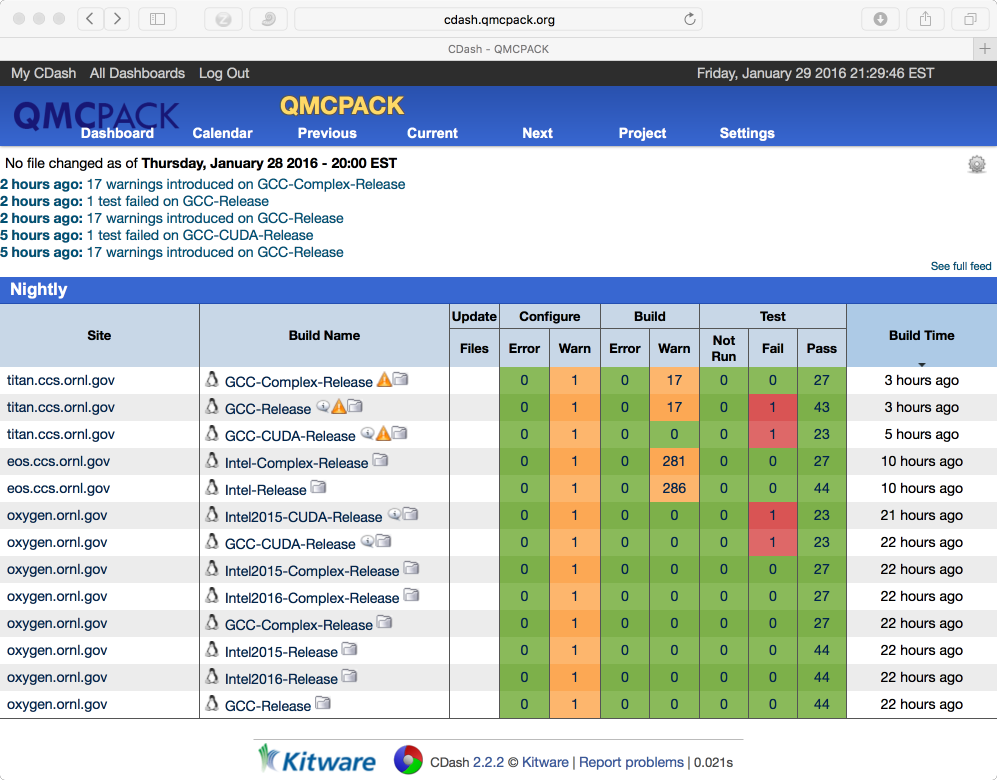
\includegraphics[width=10cm]{figures/QMCPACK_CDash_CTest_Results_20160129.png}
  \caption{Example test results for QMCPACK, showing data for a
    workstation (Intel, GCC, both CPU and GPU builds) and for two ORNL
    supercomputers. In this example, 4 errors were found. This
    dashboard is not yet openly accessible, but the developers hope
    to make it available at a later date.}
  \label{fig:cdash}
\end{figure}

\section{Building ppconvert, a pseudopotential format converter}
\label{sec:buildppconvert}
QMCPACK includes a utility, ppconvert, to convert between different
pseudopotential formats. Examples include effective core potential
formats (in gaussians), the UPF format used by Quantum ESPRESSO, and
the XML format used by QMCPACK itself. The utility also enables the
atomic orbitals to recomputed via a numerical density functional
calculation if they need to be reconstructed for use in an
electronic structure calculation.

To build ppconvert follow the instructions in
src/QMCTools/ppconvert/README. Currently ppconvert is not built
automatically although we expect to automate it soon. The makefile
must be updated to refer to suitable C++ compiler and link in
BLAS. Due to the small size of the calculations, optimal settings are
not essential.

\section{Installing and patching Quantum ESPRESSO}
\label{sec:buildqe}
For trial wavefunctions obtained in a plane-wave basis we mainly
support Quantum ESPRESSO. Note that ABINIT and QBox were supported historically
and could be reactivated.

Quantum ESPRESSO currently stores wavefunctions in a non-standard internal
``save'' format. To convert these to a conventional HDF5 format file
we have developed a converter, pw2qmcpack. This is an add on to the
Quantum ESPRESSO distribution.

To simplify the process of patching Quantum ESPRESSO we have developed
a script that will automatically download and patch the source
code. The patches are specific to each version. e.g. To download and
patch QE v5.3.0:
\begin{verbatim}
cd external_codes/quantum_espresso
./download_and_patch_qe5.3.0.sh
\end{verbatim}
After running the patch, you must configure Quantum ESPRESSO with
the HDF5 capability enabled, i.e.
\begin{verbatim}
cd espresso-5.3.0
./configure --with-hdf5 HDF5_DIR=/opt/local   # Specify HDF5 base directory
\end{verbatim}

The complete process is described in external\_codes/quantum\_espresso/README.

The tests involving pw.x and pw2qmcpack.x have been integrated in the test suite of QMCPACK.
By adding \texttt{-D QE\_BIN=your\_QE\_binary\_path} in the cmake command line when building your QMCPACK,
tests named with ``qe-'' prefix will be included in the test set of your build.
You can test the whole pw$\to$pw2qmcpack$\to$qmcpack workflow by
\begin{verbatim}
ctest -R qe
\end{verbatim}
See Sec.\ref{sec:integtestqe} and the testing section for more details.

\section{How to build the fastest executable version of QMCPACK}
\label{sec:buildperformance}
To build the fastest version of QMCPACK we recommend the following:
\begin{itemize}
\item Use the latest C++ compilers available for your
  system. Substantial gains have been made optimizing C++ in recent
  years.
\item Use a vendor optimized BLAS library such as Intel MKL and AMD ACML. Although
  QMC does not make extensive use of linear algebra, it is used in the
  VMC wavefunction optimizer, to apply the orbital coefficients in local basis
  calculations, and in the Slater determinant update.
\item Use a vector math library such as Intel VML.  For periodic
  calculations, the calculation of the structure factor and Ewald
  potential benefit from vectorized evaluation of sin and
  cos. Currently we only autodetect Intel VML, as provided with MKL,
  but support for MASSV and AMD LibM is included via \#defines. See,
  e.g. src/Numerics/e2iphi.h. For
  large supercells, this optimization can gain 10\% in performance.
\end{itemize}

Note that greater speedups of QMC calculations can usually be obtained by
carefully choosing the required statistics for each
investigation. i.e. Do not compute smaller error bars than necessary.

\section{Troubleshooting the installation}
\label{sec:troubleshoot}
Some tips to help troubleshoot installations of QMCPACK:
\begin{itemize}
\item First, build QMCPACK on a workstation that you control, or on any
  system that has a simple and up-to-date set of development
  tools. You can compare the results of cmake and QMCPACK on this
  system with any more difficult systems you encounter.
\item Use up to date development software, particularly a recent
  CMake.
\item Verify that the compilers and libraries that you expect are
  being configured. It is common to have multiple versions
  installed. The configure system will stop at the first version it
  finds which might not be the most recent. If this occurs, specify the appropriate
  directories and files directly (Section
  \ref{sec:cmakeoptions}). e.g. cmake -DCMAKE\_C\_COMPILER=/full/path/to/mpicc -DCMAKE\_CXX\_COMPILER=/full/path/to/mpicxx ..
\item To monitor the compiler and linker settings, use a verbose build, ``make
  VERBOSE=1''. If an individual source file fails to compile you
  can experiment by hand using the output of the verbose build to
  reconstruct the full compilation line.
\end{itemize}

If you still have problems please post to the QMCPACK Google group with full
details, or contact a developer.

\chapter{Running QMCPACK}
\label{chap:running}

\section{Command line options}
\label{sec:commandline}


\section{Input files}
\label{sec:inputs}

\section{Output files}
\label{sec:outputs}

  scalar.dat\\
  dmc.dat\\
  stat.h5\\
  config.h5

\section{Running in parallel}
\label{sec:parallelrunning}

considerations for mpi, threads, gpu.

\subsection{Use of OpenMP threads}
\label{sec:openmprunning}

\subsection{Running on GPU machines}
\label{sec:gpurunning}

The GPU version on the NVIDIA CUDA platform is fully incorporated into
the main trunk. Currently some commonly used functionalities for
solid-state and molecular systems using B-spline single-particle
orbitals is supported. A detailed description of the GPU
implementation can be found in Ref. \cite{EslerKimCeperleyShulenburger2012}.

Current GPU implementation assumes one MPI process per
GPU. Vectorization is achieved over walkers, that is, all walkers are
propagated in parallel. In each GPU kernel, loops over electrons,
atomic cores or orbitals are further vectorized to exploit an
additional level of parallelism and to allow coalesced memory access.

%---------------------------------------------------------------------------%

\subsubsection{Supported GPU features}

\begin{enumerate}

  \item Quantum Monte Carlo methods:

    \begin{enumerate}
	\item Variational Monte Carlo (VMC).
	\item Diffusion Monte Carlo (DMC).
	\item Limited support for wavefunction optimization.
    \end{enumerate}

  \item Boundary conditions:

    \begin{enumerate}
	\item Periodic and open boundary conditions are fully supported.
	\item Twist-averaged boundary condition is supported for only real-valued wavefunctions.
	\item Mixed boundary conditions and complex wavefunctions (e.g. fixed phase) are not yet supported. 
    \end{enumerate}

  \item Wavefunctions:

    \begin{enumerate}
	\item Single Slater determinants with 3D B-spline orbitals. Only real-valued wavefunctions is supported, but tiling complex orbitals to supercells is supported as long as each k-point is a multiple of half a G-vector of the supercell.
	\item Mixed basis representation in which orbitals are represented as 1D splines times spherical harmonics in spherical regions (muffin tins) around atoms, and 3D B-splines in the interstitial region.
	\item One-body and two-body Jastrows represented as 1D B-splines are supported. Note that only single-precision arithmetic is fully functional at the time of writing. 
    \end{enumerate}

  \item Interaction types:

    \begin{enumerate}
	\item Semilocal (nonlocal and local) pseudopotentials.
	\item Coulomb interaction (electron-electron, electron-ion).
	\item Model periodic Coulomb (MPC) interaction.
    \end{enumerate}

\end{enumerate}

%---------------------------------------------------------------------------%

\subsubsection{Compiling the GPU code}

To build the executable \courier{qmcapp} with GPU support, follow
these steps:

\begin{enumerate}
  
  \item  Make sure NVIDIA's CUDA compiler, nvcc, is in the search
    path. In most cases, CMake should be able to locate the nvcc
    compiler on the system automatically.
  \item 
    \begin{enumerate}
      \item Run CMake with the argument \courier{QMC\_CUDA} switched on: \\
               \courier{
           	cd build \\
           	cmake -D QMC\_CUDA=1 .. \\
           	make}

       \item[] \hspace{-0.27in} or

       \item If a CMake toolchain file is used, switch on \courier{QMC\_CUDA} by
         including this line in the toolchain file: \\
               \courier{SET (QMC\_CUDA 1)} \\
                Then compile the code as before: \\
                \courier{
         	cd build \\
        	cmake -D CMAKE\_TOOLCHAIN\_FILE=[toolchain name] .. \\
         	make \\}
    \end{enumerate}

\end{enumerate}

%---------------------------------------------------------------------------%

\subsubsection{CMake variables for adjusting CUDA code build features}

These values can be changed by passing them as CMake's command line
options with the \courier{-D} flag, or using a toolchain file to
overwrite the default values. \\

\begin{enumerate}

\item \courier{QMC\_CUDA}

\begin{tabular}{l@{: }p{4.5in}}
\courier{=0} (default) & no GPU support, build QMCPACK as a CPU code \\
\courier{=1}               & build QMCPACK with GPU support \\
\end{tabular} \\

\item \courier{CUDA\_PRECISION}

\begin{tabular}{l@{: }p{4in}}
\courier{=float} (default) & single precision arithmetics and data
                             types will be used for GPU kernels \\
\courier{=double}           & double precision arithmetics and data
                                 types will be used for GPU
                                 kernels (Warning: not fully
                                 functional!) \\
\end{tabular}

\end{enumerate}

%----------------------------------------------------------------------------%

\subsubsection{Performance consideration}

The relative speedup of the GPU implementation increases with both the number of electrons and the number of walkers running on a GPU. Typically, 128-256 walkers per GPU utilize sufficient number of threads to operate the GPU efficiently and to hide memory-access latency. 

To achieve better performance, current implementation utilizes single precision operations on most GPU calculations, except for matrix inversions where double precision is required to retain high accuracy. The single precision GPU code is as accurate as the double precision CPU code up to a certain system size. Cross checking and verification of accuracy are encouraged for systems with more than approximately 1500 electrons.

%------------------------------------------------------------------------------%

\subsubsection{Memory consideration}

In the GPU implementation, each walker has an anonymous buffer on the GPU's global memory to store temporary data associated with the wavefunctions. Therefore, the amount of memory available on a GPU limits the number of walkers and eventually the system size that it can process.

If the GPU memory is exhausted, reduce the number of walkers per GPU. Coarsening the grids of the B-splines representation (by decreasing the value of meshfactor in the input file) can also lower the memory usage, at the expense (risk) of obtaining inaccurate results. Proceed with caution if this option has to be considered.



\chapter{Units used in QMCPACK}
\label{sec:units}

Internally, QMCPACK uses atomic units throughout. Unless stated, all inputs and outputs are also in atomic units. For convenience the analysis tools offer conversions to eV, Ry, Angstrom, Bohr, etc.



\chapter{Input file overview}
\label{chap:input_overview}

This chapter introduces XML as it is used in QMCPACK's input file.  The focus is on the XML file format itself and the general structure of the input file rather than an exhaustive discussion of all keywords and structure elements.  

QMCPACK uses XML to represent structured data in its input file.  Instead of text blocks like
\begin{shaded}
\begin{verbatim}
begin project
  id     = vmc
  series = 0
end project

begin vmc
  move     = pbyp
  blocks   = 200
  steps    =  10
  timestep = 0.4
end vmc
\end{verbatim}
\end{shaded}
QMCPACK input looks like
\begin{shaded}
\begin{verbatim}
   <project id="vmc" series="0">
   </project>

   <qmc method="vmc" move="pbyp">
      <parameter name="blocks"  >  200 </parameter>
      <parameter name="steps"   >   10 </parameter>
      <parameter name="timestep">  0.4 </parameter>
   </qmc>
\end{verbatim}
\end{shaded}
XML elements start with \texttt{<element\_name>}, end with \texttt{</element\_name>}, and can be nested within each other to denote substructure (the trial wavefunction is composed of a Slater determinant and a Jastrow factor, which are each further composed of \ldots).  \texttt{id} and \texttt{series} are attributes of the \texttt{<project/>} element.  XML attributes are generally used to represent simple values, like names, integers, or real values.  Similar functionality is also commonly provided by \texttt{<parameter/>} elements like those shown above.

The overall structure of the input file reflects different aspects of the QMC simulation: the simulation cell, particles, trial wavefunction, Hamiltonian, and QMC run parameters.  A condensed version of the actual input file is shown below:
\begin{shaded}
\begin{verbatim}
<?xml version="1.0"?>
<simulation>

  <project id="vmc" series="0">
    ...
  </project>

  <qmcsystem>

    <simulationcell>
      ...
    </simulationcell>

    <particleset name="e">
      ...
    </particleset>

    <particleset name="ion0">
      ...
    </particleset>

    <wavefunction name="psi0" ... >
      ...
      <determinantset>
        <slaterdeterminant>
          ..
        </slaterdeterminant>
      </determinantset>
      <jastrow type="One-Body" ... >
         ...
      </jastrow>
      <jastrow type="Two-Body" ... >
        ...
      </jastrow>
    </wavefunction>

    <hamiltonian name="h0" ... >
      <pairpot type="coulomb" name="ElecElec" ... />
      <pairpot type="coulomb" name="IonIon"   ... />
      <pairpot type="pseudo" name="PseudoPot" ... >
        ...
      </pairpot>
    </hamiltonian>

   </qmcsystem>

   <qmc method="vmc" move="pbyp">
     <parameter name="warmupSteps">   20 </parameter>
     <parameter name="blocks"     >  200 </parameter>
     <parameter name="steps"      >   10 </parameter>
     <parameter name="timestep"   >  0.4 </parameter>
   </qmc>

</simulation>
\end{verbatim}
\end{shaded}
The omitted portions (\texttt{...}) are more fine-grained inputs such as the axes of the simulation cell, the number of up and down electrons, positions of atomic species, external orbital files, starting Jastrow parameters, and external pseudopotential files.  


\chapter{Specifying the system to be simulated}
\section{Specifying the simulation cell}
\label{chap:simulationcell}

The \ixml{simulationcell} block specifies the geometry of the cell, how the boundary conditions should be handled, and how ewald summation should be broken up.

\begin{table}[h]
\begin{center}
\begin{tabularx}{\textwidth}{l l l l l l }
\hline
\multicolumn{6}{l}{\texttt{simulationcell} element} \\
\hline
\multicolumn{2}{l}{parent elements:} & \multicolumn{4}{l}{\texttt{qmcsystem}}\\
\multicolumn{2}{l}{child  elements:} & \multicolumn{4}{l}{None}\\
\multicolumn{2}{l}{attribute      :} & \multicolumn{4}{l}{}\\
   &   \bfseries parameter name            & \bfseries datatype & \bfseries values & \bfseries default   & \bfseries description \\
\hline
   &   \texttt{lattice}  & 9 floats & any float & Must be specified & Specification of \\
   &                     &        &             &                   & lattice vectors. \\
   &   \texttt{bconds}   & string & ``p'' or ``n''  & ``n n n'' & Boundary conditions \\
   &                     &        &             &           & for each axis. \\
   &   \texttt{vacuum} & float & $\ge 1.0$ & 1.0        & Vacuum scale. \\
   &   \texttt{LR\_dim\_cutoff} & float & float & 15        & Ewald breakup distance. \\
\hline
\end{tabularx}
\end{center}
\end{table}

An example of a \ixml{simulationcell} block is given below:
\begin{lstlisting}[style=QMCPXML]
  <simulationcell>
    <parameter name="lattice">
      3.8       0.0       0.0
      0.0       3.8       0.0
      0.0       0.0       3.8
    </parameter>
    <parameter name="bconds">
       p p p
    </parameter>
    <parameter name="LR_dim_cutoff"> 20 </parameter>
  </simulationcell>
\end{lstlisting}

Here, a cubic cell 3.8 bohr on a side will be used.
This simulation will use periodic boundary conditions, and the maximum
$k$ vector will be $20/r_{wigner-seitz}$ of the cell.


\subsection{Lattice}
The cell is specified using 3 lattice vectors.


\subsection{Boundary conditions}
QMCPACK offers the capability to use a mixture of open and periodic boundary conditions.
The \ixml{bconds} parameter expects a single string of three characters separated by
spaces, \textit{e.g.} ``p p p'' for purely periodic boundary conditions. These characters control
the behavior of the $x$, $y$, and $z$, axes, respectively. Non periodic directions must be placed after the periodic ones.
Examples of valid \ixml{bconds} include:

\begin{description}
\item[``p p p''] Periodic boundary conditions. Corresponds to a 3D crystal.
\item[``p p n''] Slab geometry. Corresponds to a 2D crystal.
\item[``p n n''] Wire geometry. Corresponds to a 1D crystal.
\item[``n n n''] Open boundary conditions. Corresponds to an isolated molecule in a vacuum.
\end{description}

\subsection{Vacuum}
The vacuum option allows adding a vacuum region in slab or wire boundary conditions
(\ixml{bconds= p p n} or \ixml{bconds= p n n}, respectively). The main use is
to save memory with spline or plane-wave basis trial wavefunctions, because no basis
functions are required inside the vacuum region. For example, a large vacuum region
can be added above and below a graphene sheet without having to generate the trial
wavefunction in such a large box or to have as many splines as would otherwise
be required. Note that the trial wavefunction must still be generated in a
large enough box to sufficiently reduce periodic interactions in the underlying
electronic structure calculation.

With the vacuum option, the box used for Ewald summation increases along the axis labeled \ixml{n} by a factor of \ixml{vacuum}.
Note that all the particles remain in the original box without altering their positions. i.e. Bond lengths are not changed by this option.
The default value is 1, no change to the specified axes.

An example of a \ixml{simulationcell} block using \ixml{vacuum} is given below.
The size of the box along the z-axis increases from 12 to 18 by the vacuum scale of 1.5.
\begin{lstlisting}[style=QMCPXML]
  <simulationcell>
    <parameter name="lattice">
      3.8       0.0       0.0
      0.0       3.8       0.0
      0.0       0.0      12.0
    </parameter>
    <parameter name="bconds">
       p p n
    </parameter>
    <parameter name="vacuum"> 1.5 </parameter>
    <parameter name="LR_dim_cutoff"> 20 </parameter>
  </simulationcell>
\end{lstlisting}

\subsection{LR\_dim\_cutoff}
When using periodic boundary conditions direct calculation of the Coulomb energy is
not well behaved. As a result, QMCPACK uses an optimized Ewald summation technique
to compute the Coulomb interaction.\cite{Natoli1995}

In the Ewald summation, the energy is broken into short- and long-ranged terms.
The short-ranged term is computed directly in real space, while the long-ranged term is computed in reciprocal space.
\ixml{LR\_dim\_cutoff} controls where the short-ranged term ends and the long-ranged term begins.
The real-space cutoff, reciprocal-space cutoff, and \ixml{LR\_dim\_cutoff} are related via:
\[
\ixml{LR\_dim\_cutoff} = r_{c} \times k_{c}
\]
where $r_{c}$ is the Wigner-Seitz radius, and $k_{c}$ is the length of the maximum $k$-vector used in the long-ranged term.

\section{Specifying the particle set}


\chapter{Trial wavefunction specification}
\section{Introduction}
\label{sec:intro_wavefunction}

This section describes the input blocks associated with the specification of the trial wavefunction in a QMCPACK calculation. These sections are contained within the $<wavefunction > ...  </wavefunction>$ xml blocks. \textbf{Users are expected to rely on converters to generate the input blocks described in this section.} The converters and the workflows are designed such that input blocks require minimum modifications from users. Unless the workflow requires modification of wavefunction blocks (e.g. setting the cutoff in a multi determinant calculation), only expert users should directly alter them.
  
The trial wavefunction in QMCPACK has a general product form:
\begin{equation}
\Psi_T(\vec{r}) = \prod_k \Theta_k(\vec{r}),
\end{equation}
where each $\Theta_k(\vec{r})$ is a function of the electron coordinates (and possibly ionic coordinates and variational parameters). For problems involving electrons, the overall trial wavefunction must be antisymmetric with respect to electron exchange, so at least one of the functions in the product must be antisymmetric. Notice that, while QMCPACK allows for the construction of arbitrary trial wavefunctions based on the functions implemented in the code (e.g. slater determinants, jastrow functions, etc), the user must make sure that a correct wavefunction is used for the problem at hand. From here on, we assume a standard trial wavefunction for an electronic structure problem, 
\begin{equation}
\Psi_T(\vec{r}) =  \textit{A}(\vec{r}) \prod_k \textit{J}_k(\vec{r}),
\end{equation}
where $\textit{A}(\vec{r})$ is one of the antisymmetric functions: 1) slater determinant, 2) multi slater determinant, or 3) pfaffian, and $\textit{J}_k$ is any of the jastrow functions (described in section \ref{sec:jastrow}).  The antisymmetric functions are built from a set of single particle orbitals (\texttt{sposet}). QMCPACK implements 4 different types of \texttt{sposet}, described in the section below. Each \texttt{sposet} is designed for a different type of calculation, so their definition and generation varies accordingly. 

\section{Single-particle orbitals}


\subsection{Spline basis sets}
\label{sec:spo_spline}
In this section we describe the use of spline basis sets to expand the \texttt{sposet}.
Spline basis sets are designed to work seamless with plane wave DFT code, e.g.\ Quantum ESPRESSO as a trial wavefunction generator.

In QMC algorithms, all the SPOs $\{\phi(\vec{r})\}$ need to be updated every time a single electron moves.
Evaluating SPOs takes very large portion of computation time.
In principle, PW basis set can be used to express SPOs directly in QMC like in DFT.
but it introduces an unfavorable scaling due to the fact 
that the basis set size increases linearly as the system size.
For this reason, it is efficient to use a localized basis with compact
support and a good transferability from plane wave basis. 

In particular, 3D tricubic B-splines provide a basis in which only
64 elements are nonzero at any given point in space~\cite{blips4QMC}.
The one-dimensional cubic B-spline is given by,
\begin{equation}
f(x) = \sum_{i'=i-1}^{i+2} b^{i'\!,3}(x)\,\,  p_{i'},
\label{eq:SplineFunc}
\end{equation}
where $b^{i}(x)$ are the piecewise cubic polynomial basis functions
and $i = \text{floor}(\Delta^{-1} x)$ is the index of
the first grid point $\le x$.  Constructing a tensor product in each Cartesian
direction, we can represent a 3D orbital as
\begin{equation}
  \phi_n(x,y,z) = 
  \!\!\!\!\sum_{i'=i-1}^{i+2} \!\! b_x^{i'\!,3}(x) 
  \!\!\!\!\sum_{j'=j-1}^{j+2} \!\! b_y^{j'\!,3}(y) 
  \!\!\!\!\sum_{k'=k-1}^{k+2} \!\! b_z^{k'\!,3}(z) \,\, p_{i', j', k',n}.
\label{eq:TricubicValue}
\end{equation}
This allows the rapid evaluation of each orbital in constant time.
Furthermore, this basis is systematically improvable with a single spacing
parameter, so that accuracy is not compromised compared with plane wave basis.

The use of 3D tricubic B-splines greatly improves the computational efficiency.
The gain in computation time from plane wave basis set to an equivalent B-spline basis set 
becomes increasingly large as the system size grows.
On the downside, this computational efficiency comes at
the expense of increased memory use, which is easily overcome by the large
aggregate memory available per node through OpenMP/MPI hybrid QMC.

The input xml block for the spline SPOs is give in Listing~\ref{listing:splineSPOs}. A list of options is given in 
Table~\ref{table:splineSPOs}. \texttt{QMCPACK} has a very useful command line option \texttt{--save\_wfs} which allows to dump 
the real space B-spline coefficient table into a h5 file on the disk.
When the orbital transformation from k space to B-spline requires more than available amount of scratch memory on the compute nodes, 
users can perform this step on fat nodes and transfer back the h5 file for QMC calculations.

\begin{table}[h]
\begin{center}
\begin{tabularx}{\textwidth}{l l l l l l }
\hline
\multicolumn{6}{l}{\texttt{determinantset} element} \\
\hline
\multicolumn{2}{l}{parent elements:} & \multicolumn{4}{l}{\texttt{wavefunction}}\\
\multicolumn{2}{l}{child  elements:} & \multicolumn{4}{l}{\texttt{slaterdeterminant}}\\
\multicolumn{2}{l}{attribute      :} & \multicolumn{4}{l}{}\\
   &   \bfseries name              & \bfseries datatype & \bfseries values & \bfseries default   & \bfseries description \\
   &   \texttt{type}                    &  text               &   bspline   &               &  Type of \texttt{sposet}. \\
   &   \texttt{href}                    &  text               &             &               &  Path to the h5 file generated by pw2qmcpack.x. \\
   &   \texttt{tilematrix}              &  9 integers         &             &               &  Tiling matrix used to expand supercell. \\
   &   \texttt{twistnum}                &  integer            &             &               &  Index of the super twist. \\
   &   \texttt{twist}                   &  3 floats         &             &               &  Super twist. \\
   &   \texttt{meshfactor}              &  float              &  $\le 1.0$      &               &  Grid spacing ratio. \\
   &   \texttt{precision}               &  text               &  single/double  &               &  Precision of spline coefficients. \\
   &   \texttt{gpu}                    &  text               &  yes/no      &               &  GPU switch. \\
   &   \texttt{Spline\_Size\_Limit\_MB}  &  integer            &                 &             &  Limit the size of B-spline coefficient table on GPU. \\
   &   \texttt{check\_orb\_norm}     &  text                   &   yes/no      &  yes          &  Check the norms of orbitals from the input h5 file \\
   &   \texttt{source}               &  text               &   \textit{any}    &  ion0        & Particle set with the position of atom centers. \\
  \hline
\end{tabularx}
\end{center}
\caption{Options for the \texttt{determinantset} xml-block associated with B-spline single particle orbital sets.}
\label{table:splineSPOs}
\end{table}

%%\begin{lstlisting}[caption=.]
%%<sposet_builder type="bspline" href="pwscf.h5" tilematrix="2 0 0 0 2 0 0 0 2" twistnum="0"
%%                 source="i" meshfactor="1.0" precision="float" truncate="no">
%%   <sposet type="bspline" name="spo_ud" size="208" spindataset="0"/>
%%</sposet_builder>
%%<determinantset>
%%   <slaterdeterminant>
%%      <determinant id="updet" group="u" sposet="spo_ud" size="208"/>
%%      <determinant id="downdet" group="d" sposet="spo_ud" size="208"/>
%%   </slaterdeterminant>
%%</determinantset>
%%\end{lstlisting}

\begin{lstlisting}[caption=All electron Hamiltonian XML element.\label{listing:splineSPOs}]
<determinantset type="bspline" source="i" href="pwscf.h5"
                tilematrix="1 1 3 1 2 -1 -2 1 0" twistnum="-1" gpu="yes" meshfactor="0.8"
                twist="0  0  0" precision="double">
  <slaterdeterminant>
    <determinant id="updet" size="208">
      <occupation mode="ground" spindataset="0">
      </occupation>
    </determinant>
    <determinant id="downdet" size="208">
      <occupation mode="ground" spindataset="0">
      </occupation>
    </determinant>
  </slaterdeterminant>
</determinantset>
\end{lstlisting}

Additional information:
\begin{itemize}
\item \texttt{precision}. Only effective on CPU version without mixed precision, `single' is always imposed with mixed precision. Using single precision not only saves memory usage but also speeds up the B-spline evaluation. It is recommended to use single precision since we saw little chance of really compromising the accuracy of calculation.
\item \texttt{meshfactor}. It is the ratio of actual grid spacing of B-splines used in QMC calculation with respect to the original one calculated from h5. Smaller meshfactor saves memory usage but reduces accuracy. The effects are similar to reducing plane wave cutoff in DFT calculation. Use with caution! 
\item \texttt{twistnum}. If positive, it is the index. It is recommended not to take this way since the indexing may show some uncertainty. If negative, the super twist is referred by \texttt{twist}.
\item \texttt{Spline\_Size\_Limit\_MB}. Allows to distribute the B-spline coefficient table between the host and GPU memory. The compute kernels access host memory via zero-copy. Though the performance penaty introduced by it is significant but allows large calculations to go.
\end{itemize}

\subsection{Gaussian basis sets}
\label{sec:gaussianbasis}

In this section we describe the use of localized basis sets to expand the \ixml{sposet}. The general form of a single particle orbital in this case is given by:
\begin{equation}
\phi_i(\vec{r}) = \sum_k C_{i,k} \ \eta_k(\vec{r}),
\end{equation}
where $\{\eta_k(\vec{r})\}$ is a set of M atom-centered basis
functions and $C_{i,k}$ is a coefficient matrix. This \ixml{sposet}
should be used in calculations of finite systems employing an
atom-centered basis set and is typically generated by the
\textit{convert4qmc} converter.  Examples include calculations of
molecules using gaussian basis sets or slater-type basis
functions. Initial support for periodic systems is described in Sec.
\ref{chap:LCAO}. Even though this section is called "Gaussian basis
sets" (by far the most common atom-centered basis set), QMCPACK works
with any atom-centered basis set built based on either spherical
harmonic angular functions or cartesian angular expansions. The radial
functions in the basis set can be expanded in either gaussian
functions, slater-type functions or numerical radial functions.

In this section we describe the input sections for the atom-centered basis set and the \ixml{sposet} for a single slater determinant trial wavefunction. The input sections for multideterminant trial wavefunctions are described in section \ref{sec:multideterminants}. The basic structure for the input block of a single slater determinant is given in Listing \ref{listing:lcaosposet}.
A list of options for \ixml{determinantset} associated with this \ixml{sposet} is given in Table \ref{table:determinantset}.

\begin{minipage}{\linewidth}
\begin{lstlisting}[style=QMCPXML,caption=Basic input block for a single determinant trial wavefunction using a sposet expanded on an atom-centered basis set. \label{listing:lcaosposet}]
<wavefunction id="psi0" target="e">
    <determinantset>
      <basisset>
        ...
      </basisset>
      <slaterdeterminant>
        ...
      </slaterdeterminant>
    </determinantset>    
</wavefunction>
\end{lstlisting}
\end{minipage}

\begin{table}[h]
\begin{center}
\begin{tabularx}{\textwidth}{l l l l l X }
\hline
\multicolumn{6}{l}{\texttt{determinantset} element} \\
\hline
\multicolumn{2}{l}{parent elements:} & \multicolumn{4}{l}{\texttt{wavefunction}}\\
\multicolumn{2}{l}{child  elements:} & \multicolumn{4}{l}{\texttt{basisset,slaterdeterminant,sposet,multideterminant}}\\
\multicolumn{2}{l}{attribute      :} & \multicolumn{4}{l}{}\\
   &   \bfseries name              & \bfseries datatype & \bfseries values & \bfseries default   & \bfseries description \\
   &   \texttt{name}/\texttt{id}   &  text              &  \textit{any}    &  ""             & Name of determinant set. \\
   &   \texttt{type}                    &  text               &   see below   &   ""            &  Type of \texttt{sposet}. \\
   &   \texttt{keyword}             &  text               &   NMO,GTO,STO   &  NMO        & Type of orbital set generated. \\  
   &   \texttt{transform}           &  text               &   yes/no          &  yes         &  Transform to numerical radial functions?  \\
   &   \texttt{source}               &  text               &   \textit{any}    &  ion0        & Particle set with the position of atom centers. \\
   &   \texttt{cuspCorrection}  &  text               &   yes/no          &  no         & Apply cusp correction scheme to \texttt{sposet}? \\
%   &   \texttt{cuspInfo}               &  text               &   \textit{any}    &  ""             & File with saved cusp data. \\       
  \hline
\end{tabularx}
\end{center}
\caption{Options for the \ixml{determinantset} xml-block associated with atom-centered single particle orbital sets.}
\label{table:determinantset}
\end{table}

The definition of the set of atom-centered basis functions is given by the \ixml{basisset} block, while the sposet is defined within \ixml{slaterdeterminant}. The basisset input block is composed from a collection of \ixml{atomicBasisSet} input blocks, one for each atomic species in the simulation where basis functions are centered. The general structure for \ixml{basisset} and \ixml{atomicBasisSet} are given in Listing \ref{listing:basisset}, while the corresponding lists of options are given in Tables \ref{table:basisset} and \ref{table:atomicBasisSet}.

\begin{minipage}{\linewidth}
\begin{lstlisting}[style=QMCPXML,caption=Basic input block for \ixml{basisset}.\label{listing:basisset}]
      <basisset name="LCAOBSet">
        <atomicBasisSet name="Gaussian-G2" angular="cartesian" elementType="C" normalized="no">
          <grid type="log" ri="1.e-6" rf="1.e2" npts="1001"/>
          <basisGroup rid="C00" n="0" l="0" type="Gaussian">
            <radfunc exponent="5.134400000000e-02" contraction="1.399098787100e-02"/>
            ...
          </basisGroup>
          ...              
        </atomicBasisSet>
        <atomicBasisSet name="Gaussian-G2" angular="cartesian" type="Gaussian" elementType="C" normalized="no">
          ...              
        </atomicBasisSet>
        ...
      </basisset>
\end{lstlisting}
\end{minipage}

\begin{table}[h]
\begin{center}
\begin{tabularx}{\textwidth}{l l l l l X }
\hline
\multicolumn{6}{l}{\texttt{basisset} element} \\
\hline
\multicolumn{2}{l}{parent elements:} & \multicolumn{4}{l}{\texttt{determinantset}}\\
\multicolumn{2}{l}{child  elements:} & \multicolumn{4}{l}{\texttt{atomicBasisSet}}\\
\multicolumn{2}{l}{attribute      :} & \multicolumn{4}{l}{}\\
   &   \bfseries name              & \bfseries datatype & \bfseries values & \bfseries default   & \bfseries description \\
   &   \texttt{name}/\texttt{id}   &  text              &  \textit{any}    &  ""                & Name of atom-centered basis set. \\
  \hline
\end{tabularx}
\end{center}
\caption{Options for the \texttt{basisset} xml-block associated with atom-centered single particle orbital sets.}
\label{table:basisset}
\end{table}

\begin{table}[h]
\begin{center}
\begin{tabularx}{\textwidth}{l l l l l X }
\hline
\multicolumn{6}{l}{\texttt{atomicBasisSet} element} \\
\hline
\multicolumn{2}{l}{parent elements:} & \multicolumn{4}{l}{\texttt{basisset}}\\
\multicolumn{2}{l}{child  elements:} & \multicolumn{4}{l}{\texttt{grid,basisGroup}}\\
\multicolumn{2}{l}{attribute      :} & \multicolumn{4}{l}{}\\
   &   \bfseries name              & \bfseries datatype & \bfseries values & \bfseries default   & \bfseries description \\
   &   \texttt{name}/\texttt{id}   &  text              &  \textit{any}    &  ""                & Name of atomic basis set. \\
   &   \texttt{angular}               &  text              &  see below    &  default       & Type of angular functions.  \\
%   &   \texttt{type}                    &  text              &  see below    &  ""                &  Type of input radial function. \\
   &   \texttt{expandYlm}         &  text              &  see below   &  yes                &  Expand Ylm shells? \\  
   &   \texttt{expM}                  &  text              &  see below   &  yes                &  Add sign for $(-1)^{m}$? \\  
   &   \texttt{elementType/species}   &  text  &  \textit{any}    &  e                &  Atomic species where functions are centered. \\
   &   \texttt{normalized}         &  text              &  yes/no   &  yes                &  Are single particle functions normalized? \\   
  \hline
\end{tabularx}
\end{center}
\caption{Options for the \texttt{atomicBasisSet} xml-block.}
\label{table:atomicBasisSet}
\end{table}

\begin{table}[h]
\begin{center}
\begin{tabularx}{\textwidth}{l l l l l X }
\hline
\multicolumn{6}{l}{\texttt{basisGroup} element} \\
\hline
\multicolumn{2}{l}{parent elements:} & \multicolumn{4}{l}{\texttt{atomicBasisSet}}\\
\multicolumn{2}{l}{child  elements:} & \multicolumn{4}{l}{\texttt{radfunc}}\\
\multicolumn{2}{l}{attribute      :} & \multicolumn{4}{l}{}\\
   &   \bfseries name              & \bfseries datatype & \bfseries values & \bfseries default   & \bfseries description \\
   &   \texttt{rid}/\texttt{id}   &  text              &  \textit{any}    &  ""                & Name of the basisGroup. \\
   &   \texttt{type}                    &  text            &  \textit{any}    &  ""                & Type of basisGroup. \\
   &   \texttt{n/l/m/s}                 &  integer           &  \textit{any}    &  0                & Quantum numbers of basisGroup. \\
  \hline
\end{tabularx}
\end{center}
\caption{Options for the \texttt{basisGroup} xml-block.}
\label{table:basisGroup}
\end{table}

\begin{minipage}{\linewidth}
\begin{lstlisting}[style=QMCPXML,caption=Basic input block for \texttt{slaterdeterminant} with an atom-centered \texttt{sposet}.\label{listing:slaterdeterminant}]
      <slaterdeterminant>
      </slaterdeterminant>
\end{lstlisting}
\end{minipage}

\begin{table}[h]
\begin{center}
\begin{tabularx}{\textwidth}{l l l l l X }
\hline
\multicolumn{6}{l}{\texttt{} element} \\
\hline
\multicolumn{2}{l}{parent elements:} & \multicolumn{4}{l}{\texttt{}}\\
\multicolumn{2}{l}{child  elements:} & \multicolumn{4}{l}{\texttt{}}\\
\multicolumn{2}{l}{attribute      :} & \multicolumn{4}{l}{}\\
   &   \bfseries name              & \bfseries datatype & \bfseries values & \bfseries default   & \bfseries description \\
   &   \texttt{name}/\texttt{id}   &  text              &  \textit{any}    &  ""                & Name of determinant set \\
   &   \texttt{}                    &  text              &  \textit{any}    &  ""                &  \\
  \hline
\end{tabularx}
\end{center}
\end{table}

\subsubsection{Detailed description of attributes:}

In the following, we give a more detailed description of all the options presented in the various xml-blocks described in this section. Only non-trivial attributes are described below. Those with simple yes/no options and whose description above is enough to explain the intended behavior are not included. 

\hspace{1mm} \\

\ixml{determinantset} attributes:

\begin{itemize}
\item \ixml{type} \\
Type of sposet. For atom-centered based sposets, use type="MolecularOrbital" or type="MO". Other options describe elsewhere in this manual are "spline", "composite", "pw", "heg", "linearopt", etc.
\item \ixml{keyword}/\ixml{key} \\
Type of basis set generated, which doesn't necessarily match the type of the basis set on the input block. The three possible options are: NMO (numerical molecular orbitals), GTO (gaussian-type orbitals), STO (slater-type orbitals). The default option is NMO. By default, QMCPACK will generate numerical orbitals from both GTO and STO types and use cubic or quintic spline interpolation to evaluate the radial functions. This is typically more efficient than evaluating the radial functions in the native basis (gaussians or exponents) and allows for arbitrarily large contractions without any additional cost. To force the use of the native expansion (not recommended), use GTO or STO for each type of input basis set.
\item \ixml{transform}\\
Request (or avoid) a transformation of the radial functions to NMO type. The default and recommended behavior is to transform to numerical radial functions. If \ixml{transform} is set to \textit{"yes"}, the option \ixml{keyword} is ignored.  
\item \ixml{cuspCorrection}\\
Enable (disable) the use of the cusp correction algorithm (CASINO REFERENCE) for a \ixml{basisset} built with GTO functions. The algorithm is implemented as described in (CASINO REFERENCE) and only works with transform="yes" and an input GTO basis set. No further input is needed. 
\end{itemize}

\ixml{atomicBasisSet} attributes:

\begin{itemize}
\item \ixml{name/id}\\
Name of the basis set. Names should be unique.
\item \ixml{angular}\\
Type of angular functions used in the expansion. In general, two angular basis functions are allowed: "spherical" (for spherical Ylm functions) and "cartesian" (for functions of the type $x^{n}y^{m}z^{l}$).  
%\item \ixml{type}\\ Type of input radial functions. Options are: "Numerical" (for radial functions on a numerical radial grid), "Gaussian" (for an expansion in gaussian functions) and "" 
\item \ixml{expandYlm}\\
Determines whether each basis group is expanded across the corresponding shell of m values (for spherical type) or consistent powers (for cartesian functions). Options:
\begin{itemize}
\item "No": Do not expand angular functions across corresponding angular shell.
\item "Gaussian": Expand according to Gaussian03 format. This function is only compatible with angular="spherical". For a given input (l,m), the resulting order of the angular functions becomes: (1,-1,0) for l=1 and (0,1,-1,2,-2,...,l,-l) for general l.
\item "Natural": Expand angular functions according to (-l,-l+1,...,l-1,l). 
\item "Gamess": Expand according to Gamess' format for cartesian functions. Notice that this option is only compatible with angular="cartesian". If angular="cartesian" is used, this option is not necessary.
\end{itemize}
\item \ixml{expM}\\ 
Determines whether the sign of the spherical Ylm function associated with m ($-1^{m}$) is included in the coefficient matrix or not.
\item \ixml{elementType/species}\\
Name of the species where basis functions are centered. Only one atomicBasisSet block is allowed per species. Additional blocks are ignored. The corresponding species must exist in the \ixml{particleset} given as the \ixml{source} option to \ixml{determinantset}. Basis functions for all the atoms of the corresponding species are included in the basis set, based on the order of atoms in the \ixml{particleset}.
\end{itemize}

\ixml{basisGroup} attributes:

\begin{itemize}
\item \ixml{type}\\
  Type of input basis radial function. Notice that this refers to the type of radial function in the input xml-block, which might not match the radial function generated internally and used in the calculation (if \ixml{transform} is set to "yes"). Also notice that different \ixml{basisGroup} blocks within a given \ixml{atomicBasisSet} can have different \ixml{type}.
\item \ixml{n/l/m/s}\\
  Quantum numbers of the basis function. Notice that if
\ixml{expandYlm} is set to \textit{"yes"} in \ixml{atomicBasisSet}, a
full shell of basis functions with the appropriate values of
\textit{"m"} will be defined for the corresponding value of
\textit{"l"}. Otherwise a single basis function will be given for the
specific combination of \textit{"(l,m)"}.
\end{itemize}

\ixml{radfunc} attributes for \ixml{type}=\textit{"Gaussian"}:

\begin{itemize}
\item \ixml{TBDoc}\\
\end{itemize}a

\ixml{slaterdeterminant} attributes:

\begin{itemize}
\item \ixml{TBDoc}\\
\end{itemize}




\subsection{Plane-wave basis sets}
\label{sec:pwbasis}

\subsection{Homogeneous electron gas}
\label{sec:hegbasis}

The interacting Fermi liquid has its own special \ixml{determinantset} for filling up a
Fermi surface.  The shell number can be specified separately for both spin-up and spin-down.
This determines how many electrons to include of each time; only closed shells are currently
implemented.  The shells are filled according to the rules of a square box; if other lattice
vectors are used, the electrons might not fill up a complete shell.

This following example can also be used for Helium simulations by specifying the
proper pair interaction in the Hamiltonian section. 

\begin{lstlisting}[style=QMCPXML,caption=2D Fermi liquid example: particle specification ]
<qmcsystem>
<simulationcell name="global">
<parameter name="rs" pol="0" condition="74">6.5</parameter>
<parameter name="bconds">p p p</parameter>
<parameter name="LR_dim_cutoff">15</parameter>
</simulationcell>
<particleset name="e" random="yes">
<group name="u" size="37">
<parameter name="charge">-1</parameter>
<parameter name="mass">1</parameter>
</group>
<group name="d" size="37">
<parameter name="charge">-1</parameter>
<parameter name="mass">1</parameter>
</group>
</particleset>
</qmcsystem>
\end{lstlisting}

\begin{lstlisting}[style=QMCPXML,caption=2D Fermi liquid example (Slater Jastrow wavefunction) ]
<qmcsystem>
  <wavefunction name="psi0" target="e">
      <determinantset type="electron-gas" shell="7" shell2="7" randomize="true">
  </determinantset>
      <jastrow name="J2" type="Two-Body" function="Bspline" print="no">
        <correlation speciesA="u" speciesB="u" size="8" cusp="0">
          <coefficients id="uu" type="Array" optimize="yes"> 
        </correlation>
        <correlation speciesA="u" speciesB="d" size="8" cusp="0">
          <coefficients id="ud" type="Array" optimize="yes"> 
        </correlation>
      </jastrow>
\end{lstlisting}



\section{Jastrow Factors}
\label{sec:jastrow}

Jastrow factors are among the simplest and most effective ways of including
dynamical correlation in the trial many body wavefunction.  The resulting many body
wavefunction is expressed as the product of an antisymmetric (in the case
of Fermions) or symmetric (for Bosons) part and a correlating jastrow factor
like so:
\begin{equation}
\Psi(\vec{R}) = \mathcal{A}(\vec{R}) \exp\left[J(\vec{R})\right]
\end{equation}

In this section we will detail the types and forms of Jastrow factor used 
in QMCPACK.  Note that each type of Jastrow factor needs to be specified using
its own individual jastrow XML element.  For this reason, we have repeated the
specification of the jastrow tag in each section, with specialization for the
options available for that given type of jastrow.

\subsection{One-body Jastrow functions}
\label{sec:onebodyjastrow}
The one-body Jastrow factor is a form that allows for the direct inclusion
of correlations between particles that are included in the wavefunction with
particles that are not explicitly part of it.  The most common example of
this are correlations between electrons and ions.  

The jastrow function is specified within a \texttt{wavefunction} element
and must contain one or more \texttt{correlation} elements specifying
additional parameters as well as the actual coefficients. Section
\ref{sec:1bjsplineexamples} gives examples of the typical nesting of
\texttt{jastrow}, \texttt{correlation}, and \texttt{coefficient} elements.

\subsubsection{Input Specification}

\begin{table}[h]
\begin{center}
\begin{tabular}{l c c c l }
\hline
\multicolumn{5}{l}{Jastrow element} \\
\hline
\bfseries name & \bfseries datatype & \bfseries values & \bfseries defaults  & \bfseries description \\
\hline
name & text &    & (required) & Unique name for this Jastrow function \\
type & text & One-body & (required) & Define a one-body function \\ 
function & text & Bspline & (required) & BSpline Jastrow \\
             & text & pade2 & & Pade form \\
             & text & \ldots & & \ldots \\
source & text & name & (required) & name of attribute of classical particle set \\ 
print & text & yes / no & yes & jastrow factor printed in external file?\\
  \hline
\multicolumn{5}{l}{elements}\\ \hline
& Correlation & & & \\ \hline
\multicolumn{5}{l}{Contents}\\ \hline
& (None)  & & &  \\ \hline
\end{tabular}
%\end{tabular*}
\end{center}
\end{table}

To be more concrete, the one-body jastrow factors used to describe correlations
between electrons and ions take the form below
\begin{equation}
J1=\sum_I^{ion0}\sum_i^e u_{ab}(|r_i-R_I|)
\end{equation}
where I runs over all of the ions in the calculation, i runs over the electrons
and $u_{ab}$ describes the functional form of the correlation between them.
Many different forms of $u_{ab}$ are implemented in QMCPACK.  We will detail 
two of the most common ones below.
\subsubsection{Spline form}
\label{sec:onebodyjastrowspline}

The one-body spline Jastrow function is the most commonly used one-body Jastrow for solids. This form 
was first described and used in \cite{EslerKimCeperleyShulenburger2012}.  
Here $u_{ab}$ is an interpolating 1D Bspline (tricublc spline on a linear grid) between zero distance and $r_{cut}$. In 3D periodic systems 
the default cutoff distance is the Wigner Seitz cell radius. For other periodicities including isolated 
molecules the $r_{cut}$ must be specified. The cusp can be set.   $r_i$ 
and $R_I$ are most commonly the electron and ion positions, but any particlesets that can provide the 
needed centers can be used.

\paragraph{Input Specification}
\begin{table}[h]
\begin{center}
\begin{tabular}{l c c c l }
\hline
\multicolumn{5}{l}{Correlation element} \\
\hline
\bfseries name & \bfseries datatype & \bfseries values & \bfseries defaults & \bfseries description \\
\hline
elementType & text & name & see below & Classical particle target  \\
speciesA & text & name & see below & Classical particle target \\
speciesB & text & name & see below & Quantum species target \\
size & integer & $> 0$ & (required) & Number of coefficients \\
rcut & real & $> 0$ & see below & Distance at which the correlation goes to 0 \\
cusp & real & $\ge 0$ & 0 & Value for use in Kato cusp condition \\
spin & text & yes or no & no & Spin dependent jastrow factor \\
\hline
\multicolumn{5}{l}{elements}\\ \hline
& Coefficients & & & \\ \hline
\multicolumn{5}{l}{Contents}\\ \hline
& (None)  & & &  \\ \hline
\end{tabular}
%\end{tabular*}
\end{center}
\end{table}

Additional information:

 \begin{itemize}
 \item \texttt{elementType, speciesA, speciesB, spin}.  For a spin independent Jastrow factor (spin = ``no'')
elementType should be the name of the group of ions in the classical particleset to which the quantum
particles should be correlated.  For a spin dependent Jastrow factor (spin = ``yes'') set speciesA to the
group name in the classical particleset and speciesB to the group name in the quantum particleset.
 \item \texttt{rcut}. The cutoff distance for the function in atomic units (bohr). 
For 3D fully periodic systems this parameter is optional and a default of the Wigner 
Seitz cell radius is used. Otherwise this parameter is required.
 \item \texttt{cusp}. The one body jastrow factor can be used to make the wavefunction
satisfy the electron-ion cusp condition\cite{kato}.  In this case, the derivative of the jastrow
factor as the electron approaches the nucleus will be given by:
\begin{equation}
\left(\frac{\partial J}{\partial r_{iI}}\right)_{r_{iI} = 0} = -Z
\end{equation}
Note that if the antisymmetric part of the wavefunction satisfies the electron-ion cusp
condition (for instance by using single particle orbitals that respect the cusp condition)
or if a non-divergent pseudopotential is used that the Jastrow should be cuspless at the 
nucleus and this value should be kept at its default of 0.
 \end{itemize}


\begin{table}[h]
\begin{center}
\begin{tabular}{l c c c l }
\hline
\multicolumn{5}{l}{Coefficients element} \\
\hline
\bfseries name & \bfseries datatype & \bfseries values & \bfseries defaults & \bfseries description \\
\hline
id & text & & (required) & Unique identifier \\
type & text & Array & (required) & \\
optimize & text & yes or no & yes & if no, values are fixed in optimizations \\
\hline
\multicolumn{5}{l}{elements}\\ \hline
(None) & & & \\ \hline
\multicolumn{5}{l}{Contents}\\ \hline
 (no name) & real array & & zeros & Jastrow coefficients \\ \hline
\end{tabular}
%\end{tabular*}
\end{center}
\end{table}


\paragraph{Example use cases}
\label{sec:1bjsplineexamples}

Specify a spin-independent function with four parameters. Because rcut  is not 
specified, the default cutoff of the Wigner Seitz cell radius is used; this 
Jastrow must be used with a 3D periodic system such as a bulk solid. The name of 
the particleset holding the ionic positions is "i".
\begin{lstlisting}[language=xml]
<jastrow name="J1" type="One-Body" function="Bspline" print="yes" source="i">
 <correlation elementType="C" cusp="0.0" size="4">
   <coefficients id="C" type="Array"> 0  0  0  0  </coefficients>
 </correlation>
</jastrow>
\end{lstlisting}

Specify a spin-dependent function with seven upspin and seven downspin parameters. 
The cutoff distance is set to 6 atomic units.  Note here that the particleset holding
the ions is labeled as ion0 rather than ``i'' in the other example.  Also in this case
the ion is Lithium with a coulomb potential, so the cusp condition is satisfied by 
setting cusp="d".
\begin{lstlisting}[language=xml]
<jastrow name="J1" type="One-Body" function="Bspline" source="ion0" spin="yes">
  <correlation speciesA="Li" speciesB="u" size="7" rcut="6">
    <coefficients id="eLiu" cusp="3.0" type="Array"> 
    0.0 0.0 0.0 0.0 0.0 0.0 0.0
    </coefficients>
  </correlation>
  <correlation speciesA="C" speciesB="d" size="7" rcut="6">
    <coefficients id="eLid" cusp="3.0" type="Array"> 
    0.0 0.0 0.0 0.0 0.0 0.0 0.0
    </coefficients>
  </correlation>
</jastrow>
\end{lstlisting}


\subsubsection{Pade form}
\label{sec:onebodyjastrowpade}

While the spline Jastrow factor is the most flexible and most commonly used form implemented in \qmcpack, 
there are times where its flexibility can make it difficult to optimize.  As an example, a spline jastrow
with a very large cutoff may be difficult to optimize for isolated systems like molecules due to the small
number of samples that will be present in the tail of the function.  In such cases, a simpler functional
form may be advantageous.  The second order Pade jastrow factor, given in Eq.\ref{padeeqn} is a good choice 
in such cases.  
\begin{equation}
\label{padeeqn}
u_{ab}(r) = \frac{a*r+c*r^2}{1+b*r}
\end{equation}
Unlike the spline jastrow factor which includes a cutoff, this form has an infinite range and for every particle
pair (subject to the minimum image convention) it will be applied.  It also is a cuspless jastrow factor,
so it should either be used in combination with a single particle basis set that contains the proper cusp or
with a smooth pseudopotential.

\paragraph{Input Specification}
\begin{table}[h]
\begin{center}
\begin{tabular}{l c c c l }
\hline
\multicolumn{5}{l}{Correlation element} \\
\hline
\bfseries name & \bfseries datatype & \bfseries values & \bfseries defaults & \bfseries description \\
\hline
elementType & text & name & see below & Classical particle target  \\
\hline
\multicolumn{5}{l}{elements}\\ \hline
& Coefficients & & & \\ \hline
\multicolumn{5}{l}{Contents}\\ \hline
& (None)  & & &  \\ \hline
\end{tabular}
%\end{tabular*}
\end{center}
\end{table}

\begin{table}[h]
\begin{center}
\begin{tabular}{l c c c l }
\hline
\multicolumn{5}{l}{parameter element} \\
\hline
\bfseries name & \bfseries datatype & \bfseries values & \bfseries defaults & \bfseries description \\
\hline
id & string & name & (required) & name for variable \\
name & string & A or B or C & (required) & see Eq.\ref{padeeqn}\\
optimize & text & yes or no & yes & if no, values are fixed in optimizations \\
\hline
\multicolumn{5}{l}{elements}\\ \hline
(None) & & & \\ \hline
\multicolumn{5}{l}{Contents}\\ \hline
 (no name) & real & parameter value & (required) & Jastrow coefficients \\ \hline
\end{tabular}
%\end{tabular*}
\end{center}
\end{table}

\paragraph{Example use case}
\label{sec:1bjpadeexamples}

Specify a spin independent function with independent jastrow factors for two different species (Li and H).
The name of the particleset holding the ionic positions is "i".
\begin{lstlisting}[style=XML]
<jastrow name="J1" function="pade2" type="One-Body" print="yes" source="i">
  <correlation elementType="Li">
    <var id="LiA" name="A">  0.34 </var>
    <var id="LiB" name="B"> 12.78 </var>
    <var id="LiC" name="C">  1.62 </var>
  </correlation>
  <correlation elementType="H"">
    <var id="HA" name="A">  0.14 </var>
    <var id="HB" name="B"> 6.88 </var>
    <var id="HC" name="C"> 0.237 </var>
  </correlation>
</jastrow>
\end{lstlisting}


\subsection{Two-body Jastrow functions}
The two-body Jastrow factor is a form that allows for the explicit inclusion
of dynamic correlation between two particles included in the wavefunction.  It
is almost always given in a spin dependent form so as to satisfy the Kato cusp
condition between electrons of different spins\cite{kato}.

 The two body jastrow function is specified within a \texttt{wavefunction} element
and must contain one or more correlation elements specifying additional parameters
as well as the actual coefficients.  Section \ref{sec:2bjsplineexamples} gives 
examples of the typical nesting of \texttt{jastrow}, \texttt{correlation} and
\texttt{coefficient} elements.

\subsubsection{Input Specification}

\begin{table}[h]
\begin{center}
\begin{tabular}{l c c c l }
\hline
\multicolumn{5}{l}{Jastrow element} \\
\hline
\bfseries name & \bfseries datatype & \bfseries values & \bfseries defaults  & \bfseries description \\
\hline
name & text &    & (required) & Unique name for this Jastrow function \\
type & text & Two-body & (required) & Define a one-body function \\ 
function & text & Bspline & (required) & BSpline Jastrow \\
print & text & yes / no & yes & jastrow factor printed in external file?\\
  \hline
\multicolumn{5}{l}{elements}\\ \hline
& Correlation & & & \\ \hline
\multicolumn{5}{l}{Contents}\\ \hline
& (None)  & & &  \\ \hline
\end{tabular}
%\end{tabular*}
\end{center}
\end{table}

The two-body jastrow factors used to describe correlations between electrons take the form
\begin{equation}
J2=\sum_i^{e}\sum_{j>i}^{e} u_{ab}(|r_i-r_j|)
\end{equation}

The most commonly used form of two body jastrow factor supported by the code is a splined
jastrow factor, with many similarities to the one body spline jastrow.

\subsubsection{Spline form}
\label{sec:twobodyjastrowspline}

The two-body spline Jastrow function is the most commonly used two-body Jastrow for solids. This form 
was first described and used in \cite{EslerKimCeperleyShulenburger2012}.  
Here $u_{ab}$ is an interpolating 1D Bspline (tricublc spline on a linear grid) between 
zero distance and $r_{cut}$. In 3D periodic systems 
the default cutoff distance is the Wigner Seitz cell radius. For other periodicities including isolated 
molecules the $r_{cut}$ must be specified.  $r_i$ and $r_j$ are typically electron positions.  The cusp 
condition as $r_i$ approaches $r_j$ is set by the relative spin of the electrons.

\FloatBarrier
\paragraph{Input Specification}

\FloatBarrier
\begin{table}[h!]
\begin{center}
\begin{tabular}{l c c c l }
\hline
\multicolumn{5}{l}{Correlation element} \\
\hline
\bfseries name & \bfseries datatype & \bfseries values & \bfseries defaults & \bfseries description \\
\hline
speciesA & text & u or d & (required) & Quantum species target \\
speciesB & text & u or d & (required) & Quantum species target \\
size & integer & $> 0$ & (required) & number of coefficients \\
rcut & real & $> 0$ & see below & distance at which the correlation goes to 0 \\
spin & text & yes or no & no & spin dependent jastrow factor \\
\hline
\multicolumn{5}{l}{elements}\\ \hline
& Coefficients & & & \\ \hline
\multicolumn{5}{l}{Contents}\\ \hline
& (None)  & & &  \\ \hline
\end{tabular}
%\end{tabular*}
\end{center}
\end{table}

\FloatBarrier

Additional information:
\begin{itemize}
\item \texttt{speciesA, speciesB} The scale function u(r) is defined for species pairs uu and ud.  
There is no need to define ud or dd since uu=dd and ud=du.  The cusp condition is computed internally 
based on the charge of the quantum particles.
\end{itemize}

\begin{table}[h]
\begin{center}
\begin{tabular}{l c c c l }
\hline
\multicolumn{5}{l}{Coefficients element} \\
\hline
\bfseries name & \bfseries datatype & \bfseries values & \bfseries defaults & \bfseries description \\
\hline
id & text & & (required) & Unique identifier \\
type & text & Array & (required) & \\
optimize & text & yes or no & yes & if no, values are fixed in optimizations \\
\hline
\multicolumn{5}{l}{elements}\\ \hline
(None) & & & \\ \hline
\multicolumn{5}{l}{Contents}\\ \hline
 (no name) & real array & & zeros & Jastrow coefficients \\ \hline
\end{tabular}
%\end{tabular*}
\end{center}
\end{table}

\paragraph{Example use cases}
\label{sec:2bjsplineexamples}

Specify a spin-dependent function with 4 parameters for each channel.  In this case, the cusp is set at 
a radius of 4.0 bohr (rather than to the default of the Wigner Seitz cell radius).  Also, in this example,
the coefficients are set to not be optimized during an optimization step.

\begin{lstlisting}
<jastrow name="J2" type="Two-Body" function="Bspline" print="yes">
  <correlation speciesA="u" speciesB="u" size="8" rcut="4.0">
    <coefficients id="uu" type="Array" optimize="no"> 0.2309049836 0.1312646071 0.05464141356 0.01306231516</coefficients>
  </correlation>
  <correlation speciesA="u" speciesB="d" size="8" rcut="4.0">
    <coefficients id="ud" type="Array" optimize="no"> 0.4351561096 0.2377951747 0.1129144262 0.0356789236</coefficients>
  </correlation>
</jastrow>
\end{lstlisting}


\subsection{Three-body Jastrow functions}
Explicit three body correlations can be included in the wavefunction via the three-body
jastrow factor.

\section{Multideterminant wavefunctions}

\section{Backflow wavefunctions}


\chapter{Hamiltonian and Observables}
\label{chap:hamiltobs}


\qmcpack is capable of the simultaneous measurement of the Hamiltonian and many other quantum operators.  The Hamiltonian attains a special status among the available operators (also referred to as observables) because it ultimately generates all available information regarding the quantum system.  This is evident from an algorithmic standpoint as well since the Hamiltonian (embodied in the the projector) generates the imaginary time dynamics of the walkers in DMC and RMC. 

This section covers how the Hamiltonian can be specified, component by component, by the user in the XML format native to \qmcpack.  It also covers the input structure of statistical estimators corresponding to quantum observables such as the density, the static structure factor, and forces.



\section{The Hamiltonian}

The many-body Hamiltonian in Hartree units is given by
\begin{align}
  \hat{H} = -\sum_i\frac{1}{2m_i}\nabla_i^2 + \sum_iv^{ext}(r_i) + \sum_{i<j}v^{qq}(r_i,r_j)   + \sum_{i\ell}v^{qc}(r_i,r_\ell)   + \sum_{\ell<m}v^{cc}(r_\ell,r_m).  
\end{align}
Here, the sums indexed by $i/j$ are over quantum particles, while $\ell/m$ are reserved for classical particles.  Often the quantum particles are electrons and the classical particles are ions, though \qmcpack is not limited in this way.  The mass of each quantum particle is denoted $m_i$, $v^{qq}/v^{qc}/v^{cc}$ are pair potentials between quantum-quantum/quantum-classical/classical-classical particles, and $v^{ext}$ denotes a purely external potential.

\qmcpack is designed modularly so that any potential can be supported with minimal additions to the code base.  Potentials currently supported include Coulomb interactions in open and periodic boundary conditions, the modified periodic coulomb (MPC) potential, non-local pseudopotentials, helium pair potentials, and various model potentials such as hard sphere, gaussian, and modified Poschl-Teller.

Reference information and examples for the \texttt{<hamiltonian/>} XML element is provided below.  Detailed descriptions of the input for individual potentials is given in the sections that follow.  

% hamiltonian element
%  dev notes
%    Hamiltonian element read
%      HamiltonianPool::put
%        reads attributes: id name role target 
%          id/name is passed to QMCHamiltonian
%          role selects the primary hamiltonian
%          target associates to quantum particleset
%      HamiltonianFactory::build
%        reads attributes: type source default
%    HamiltonianFactory cloning may be flawed for non-electron systems
%      see HamiltonianFactory::clone
%        aCopy->renameProperty(``e'',qp->getName());
%        aCopy->renameProperty(psiName,psi->getName());
%      the renaming may not work if dynamic particleset.name!=''e''
%   lots of xml inputs are simply ignored if do not explicitly match (fix! here and elsewhere in the build tree)

\FloatBarrier
\begin{table}[h]
\begin{center}
\begin{tabularx}{\textwidth}{l l l l l l }
\hline
\multicolumn{6}{l}{\texttt{hamiltonian} element} \\
\hline
\multicolumn{2}{l}{parent elements:} & \multicolumn{4}{l}{\texttt{simulation, qmcsystem}}\\
\multicolumn{2}{l}{child  elements:} & \multicolumn{4}{l}{\texttt{pairpot extpot estimator constant}(deprecated)}\\
\multicolumn{2}{l}{attributes}  & \multicolumn{4}{l}{}\\
   &   \bfseries name     & \bfseries datatype & \bfseries values & \bfseries default & \bfseries description \\
   & \texttt{name/id}$^o$ &  text              & \textit{anything}& h0                & Unique id for this Hamiltonian instance  \\
   & \texttt{type}$^o$    &  text              &                  & generic           & \textit{No current function}             \\
   & \texttt{role}$^o$    &  text              & primary/extra    & extra             & Designate as primary Hamiltonian or not  \\
   & \texttt{source}$^o$  &  text              & \texttt{particleset.name} & i        & Identify classical particleset           \\
   & \texttt{target}$^o$  &  text              & \texttt{particleset.name} & e        & Identify quantum particleset             \\
   & \texttt{default}$^o$ &  boolean           & yes/no           & yes               & Include kinetic energy term implicitly   \\
  \hline
\end{tabularx}
\end{center}
\end{table}
\FloatBarrier

Additional information:
\begin{itemize}
  \item{\textbf{target:} Must be set to the name of the quantum particeset.  The default value is typically sufficient.  In normal usage, no other attributes are provided.}
\end{itemize}

% All-electron hamiltonian element
\begin{lstlisting}[caption=All electron Hamiltonian XML element.]
<hamiltonian target="e">
  <pairpot name="ElecElec" type="coulomb" source="e" target="e"/>
  <pairpot name="ElecIon"  type="coulomb" source="i" target="e"/>
  <pairpot name="IonIon"   type="coulomb" source="i" target="i"/>
</hamiltonian>
\end{lstlisting}


% Pseudopotential hamiltonian element
\begin{lstlisting}[caption=Pseudopotential Hamiltonian XML element.]
<hamiltonian target="e">
  <pairpot name="ElecElec"  type="coulomb" source="e" target="e"/>
  <pairpot name="PseudoPot" type="pseudo"  source="i" wavefunction="psi0" format="xml">
    <pseudo elementType="Li" href="Li.xml"/>
    <pseudo elementType="H" href="H.xml"/>
  </pairpot>
  <pairpot name="IonIon"    type="coulomb" source="i" target="i"/>
</hamiltonian>
\end{lstlisting}


\section{Pair potentials}

Many pair potentials are supported.  Though only the most commonly used pair potentials are covered in detail in this section, all currently available potentials are listed briefly below.  If a potential you desire is not covered below, or is not present at all, feel free to contact the developers.

% pairpot element
\FloatBarrier
\begin{table}[h]
\begin{center}
\begin{tabularx}{\textwidth}{l l l l l l }
\hline
\multicolumn{6}{l}{\texttt{pairpot} factory element} \\
\hline
\multicolumn{2}{l}{parent elements:} & \multicolumn{4}{l}{\texttt{hamiltonian}}\\
\multicolumn{2}{l}{type   selector:} & \multicolumn{4}{l}{\texttt{type} attribute}\\
\multicolumn{2}{l}{type   options: } & \multicolumn{2}{l}{coulomb           } & \multicolumn{2}{l}{Coulomb/Ewald potential}\\
\multicolumn{2}{l}{                } & \multicolumn{2}{l}{pseudo            } & \multicolumn{2}{l}{Semilocal pseudopotential}\\
\multicolumn{2}{l}{                } & \multicolumn{2}{l}{mpc               } & \multicolumn{2}{l}{Modified Periodic Coulomb interaction/correction}\\
\multicolumn{2}{l}{                } & \multicolumn{2}{l}{cpp               } & \multicolumn{2}{l}{Core polarization potential}\\
\multicolumn{2}{l}{                } & \multicolumn{2}{l}{numerical/*num*   } & \multicolumn{2}{l}{Numerical radial potential}\\
\multicolumn{2}{l}{                } & \multicolumn{2}{l}{skpot             } & \multicolumn{2}{l}{\textit{Unknown}}\\
\multicolumn{2}{l}{                } & \multicolumn{2}{l}{vhxc              } & \multicolumn{2}{l}{Exchange correlation potential (external)}\\
\multicolumn{2}{l}{                } & \multicolumn{2}{l}{jellium           } & \multicolumn{2}{l}{Atom-centered spherical jellium potential}\\
\multicolumn{2}{l}{                } & \multicolumn{2}{l}{hardsphere        } & \multicolumn{2}{l}{Hard sphere potential}\\
\multicolumn{2}{l}{                } & \multicolumn{2}{l}{gaussian          } & \multicolumn{2}{l}{Gaussian potential}\\
\multicolumn{2}{l}{                } & \multicolumn{2}{l}{modpostel         } & \multicolumn{2}{l}{Modified Poschl-Teller potential}\\
\multicolumn{2}{l}{                } & \multicolumn{2}{l}{huse              } & \multicolumn{2}{l}{Huse quintic potential}\\
\multicolumn{2}{l}{                } & \multicolumn{2}{l}{modInsKE          } & \multicolumn{2}{l}{Model insulator kinetic energy}\\
\multicolumn{2}{l}{                } & \multicolumn{2}{l}{oscillatory       } & \multicolumn{2}{l}{\textit{Unknown}}\\
\multicolumn{2}{l}{                } & \multicolumn{2}{l}{LJP\_smoothed     } & \multicolumn{2}{l}{Helium pair potential}\\
\multicolumn{2}{l}{                } & \multicolumn{2}{l}{HeSAPT\_smoothed  } & \multicolumn{2}{l}{Helium pair potential}\\
\multicolumn{2}{l}{                } & \multicolumn{2}{l}{HFDHE2\_Moroni1995} & \multicolumn{2}{l}{Helium pair potential}\\
\multicolumn{2}{l}{                } & \multicolumn{2}{l}{HFDHE2            } & \multicolumn{2}{l}{Helium pair potential}\\
\multicolumn{2}{l}{                } & \multicolumn{2}{l}{eHe               } & \multicolumn{2}{l}{Helium-electron pair potential}\\
\multicolumn{2}{l}{shared attributes:} & \multicolumn{4}{l}{}\\
   &   \bfseries name     & \bfseries datatype & \bfseries values & \bfseries default   & \bfseries description \\
   &   \texttt{type}$^r$      &  text              & \textit{See above}        & 0                   & Select pairpot type         \\
   &   \texttt{name}$^r$      &  text              & \textit{anything}         & any                 & Unique name for this pairpot\\
   &   \texttt{source}$^r$    &  text              & \texttt{particleset.name} &\texttt{hamiltonian.target}& Identify interacting particles\\
   &   \texttt{target}$^r$    &  text              & \texttt{particleset.name} &\texttt{hamiltonian.target}& Identify interacting particles  \\
   &   \texttt{units}$^o$     &  text              &                           & hartree             & \textit{No current function}  \\
\hline
\end{tabularx}
\end{center}
\end{table}
\FloatBarrier

Additional information:
\begin{itemize}
  \item{\textbf{type:} Used to select the desired pair potential.  Must be selected from the list of type options above.}
  \item{\textbf{name:} A unique name used to identify this pair potential.  Block averaged output data will appear under this name in \texttt{scalar.dat} and/or \texttt{stat.h5} files.}
  \item{\textbf{source/target:}  These specify the particles involved in a pair interaction.  If an interaction is between classical (e.g. ions) and quantum (e.g. electrons), \texttt{source}/\texttt{target} should be the name of the classical/quantum particleset.}
  \item{Only \texttt{coulomb, pseudo, mpc} are described in detail below.  The older or less used types (\texttt{cpp, numerical, jellium, hardsphere, gaussian, huse, modpostel, oscillatory, skpot, vhxc, modInsKE, LJP\_smoothed, HeSAPT\_smoothed, HFDHE2\_Moroni1995, eHe, HFDHE2}) are not covered.}
  \dev{
  \item{Available only if \texttt{QMC\_BUILD\_LEVEL>2} and \texttt{QMC\_CUDA} is not defined: \texttt{hardsphere, gaussian, huse, modpostel, oscillatory, skpot}.}
  \item{Available only if \texttt{OHMMS\_DIM==3}: \texttt{mpc, vhxc, pseudo}.}
  \item{Available only if \texttt{OHMMS\_DIM==3} and \texttt{QMC\_BUILD\_LEVEL>2} and \texttt{QMC\_CUDA} is not defined: \texttt{cpp, LJP\_smoothed, HeSAPT\_smoothed, HFDHE2\_Moroni1995, eHe, jellium, HFDHE2, modInsKE}.}
  }
\end{itemize}


% physical read by coulomb potentials
% potential is only for pressure estimator



% pairpot instances

%   do coulomb, pseudo, mpc

\subsection{Coulomb potentials}

The bare Coulomb potential is used in open boundary conditions:
\begin{align}
  V_c^{open} = \sum_{i<j}\frac{q_iq_j}{\abs{r_i-r_j}}
\end{align}

When periodic boundary conditions are selected, Ewald summation is used automatically:
\begin{align}\label{eq:ewald}
  V_c^{pbc} = \sum_{i<j}\frac{q_iq_j}{\abs{r_i-r_j}} + \frac{1}{2}\sum_{L\ne0}\sum_{i,j}\frac{q_iq_j}{\abs{r_i-r_j+L}}
\end{align}
The sum indexed by $L$ is over all non-zero simulation cell lattice vectors.  In practice, the Ewald sum is broken into short and long ranged parts in a manner optimized for efficiency (see Ref. \cite{Natoli1995}) for details. 

For information on how to set the boundary conditions, consult Sec. \ref{sec:simulationcell}.


\FloatBarrier
\begin{table}[h]
\begin{center}
\begin{tabularx}{\textwidth}{l l l l l l }
\hline
\multicolumn{6}{l}{\texttt{pairpot type=coulomb} element} \\
\hline
\multicolumn{2}{l}{parent elements:} & \multicolumn{4}{l}{\texttt{hamiltonian}}\\
\multicolumn{2}{l}{child  elements:} & \multicolumn{4}{l}{\textit{None}}\\
\multicolumn{2}{l}{attributes}  & \multicolumn{4}{l}{}\\
   &   \bfseries name     & \bfseries datatype & \bfseries values & \bfseries default   & \bfseries description \\
   & \texttt{type}$^r$    &  text              & \textbf{coulomb} &                     & Must be coulomb     \\
   & \texttt{name/id}$^r$ &  text              & \textit{anything}&  ElecElec           & Unique name for interaction\\
   & \texttt{source}$^r$  &  text              & \texttt{particleset.name} &\texttt{hamiltonian.target}& Identify interacting particles\\
   & \texttt{target}$^r$  &  text              & \texttt{particleset.name} &\texttt{hamiltonian.target}& Identify interacting particles\\
   & \texttt{pbc}$^o$     &  boolean           & yes/no           & yes                 & Use Ewald summation  \\
   & \texttt{physical}$^o$&  boolean           & yes/no           & yes                 & Hamiltonian(yes)/observable(no) \\
\dev{& \texttt{forces}      &  boolean           & yes/no           & no                  & \textit{Deprecated}             \\ }
  \hline
\end{tabularx}
\end{center}
\end{table}
\FloatBarrier

Additional information
\begin{itemize}
  \item{\textbf{type/source/target} See description for the generic \texttt{pairpot} factory element above.}
  \item{\textbf{name:} Traditional user-specified names for electron-electron, electron-ion, and ion-ion terms are \texttt{ElecElec}, \texttt{ElecIon}, and \texttt{IonIon}, respectively.  While any choice can be used, the data analysis tools expect to find columns in \texttt{*.scalar.dat} with these names.}
  \item{\textbf{pbc}: Ewald summation will not be performed if \texttt{simulationcell.bconds== n n n}, regardless of the value of \texttt{pbc}.  Similarly, the \texttt{pbc} attribute can only be used to turn off Ewald summation if \texttt{simulationcell.bconds!= n n n}.  The default value is recommended.}
  \item{\textbf{physical}: If \texttt{physical==yes}, this pair potential is included in the Hamiltonian and will factor into the \texttt{LocalEnergy} reported by QMCPACK and also in the DMC branching weight.  If \texttt{physical==no}, then the pair potential is treated as a passive observable but not as part of the Hamiltonian itself.  As such it does not contribute to the outputted \texttt{LocalEnergy}.  Regardless of the value of \texttt{physical} output data will appear in \texttt{scalar.dat} in a column headed by \texttt{name}.}
\end{itemize}


\begin{lstlisting}[caption=XML element for Coulomb interaction between electrons.]
  <pairpot name="ElecElec" type="coulomb" source="e" target="e"/>
\end{lstlisting}

\begin{lstlisting}[caption=XML element for Coulomb interaction between electrons and ions (all-electron only).]
  <pairpot name="ElecIon"  type="coulomb" source="i" target="e"/>
\end{lstlisting}

\begin{lstlisting}[caption=XML element for Coulomb interaction between ions.]
  <pairpot name="IonIon"   type="coulomb" source="i" target="i"/>
\end{lstlisting}


\subsection{Pseudopotentials}

\qmcpack supports pseudopotentials in semilocal form, which is local in the radial coordinate and non-local in angular coordinates.  When all angular momentum channels above a certain threshold ($\ell_{max}$) are well approximated by the same potential ($V_{\bar{\ell}}\equiv V_{loc}$), the pseudpotential separates into a fully local channel and an angularly-nonlocal component:
\begin{align}
  V^{PP} = \sum_{ij}\Big(V_{\bar{\ell}}(\abs{r_i-\tilde{r}_j}) + \sum_{\ell\ne\bar{\ell}}^{\ell_{max}}\sum_{m=-\ell}^\ell \operator{Y_{\ell m}}{\big[V_\ell(\abs{r_i-\tilde{r}_j}) - V_{\bar{\ell}}(\abs{r_i-\tilde{r}_j}) \big]}{Y_{\ell m}} \Big)
\end{align}  
Here the electron/ion index is $i/j$ and only one type of ion is shown for simplicity.

Evaluation of the localized pseudopotential energy $\Psi_T^{-1}V^{PP}\Psi_T$ requires additional angular integrals.  These integrals are evaluated on a randomly shifted angular grid.  The size of this grid is determined by $\ell_{max}$.  See Ref. \cite{Mitas1991} for further detail. 

\qmcpack uses the FSAtom pseudopotential file format associated with the ``Free Software Project for Atomic-scale Simulations'' initiated in 2002  (see \url{http://www.tddft.org/fsatom/manifest.php} for general information).  The FSAtom format uses XML for structured data.  Files in this format do not use a specific identifying file extension; they are simply suffixed with ``\texttt{.xml}''.  The tabular data format of CASINO is also supported.


% FSAtom format links
%   unfortunately none of the surviving links detail the format itself
% http://www.tddft.org/fsatom/index.php
% http://www.tddft.org/fsatom/programs.php
% http://www.tddft.org/fsatom/manifest.php
% http://163.13.111.58/cchu/reference/web/PseudoPotentials%20-%20FSAtom%20Wiki.htm
% http://departments.icmab.es/leem/alberto/xml/pseudo/index.html



% pseudopotential element
%   dev notes
%     attributes name, source, wavefunction, format are read in CoulombFactory.cpp  HamiltonianFactory::addPseudoPotential
%     format==''old'' refers to an old table format that is no longer supported
%     read continues in ECPotentialBuilder::put()
%       if format!=xml/old (i.e. table) qmcpack will attempt to read from *.psf files
%         in this case, <pairpot type=''pseudo'' format=''table''/>, ie there are no elements
%         if particlset groups are Li H (in order), then it looks for Li.psf and H.psf
%         what is the psf format?
%       if format==xml, normal read continues, i.e. <pseudo/> child elements are expected
%         read is not sensitive to particleset group/species ordering
%         child elements not named <pseudo/> are simply ignored (FIX!)
\FloatBarrier
\begin{table}[h]
\begin{center}
\begin{tabularx}{\textwidth}{l l l l l l }
\hline
\multicolumn{6}{l}{\texttt{pairpot type=pseudo} element} \\
\hline
\multicolumn{2}{l}{parent elements:} & \multicolumn{4}{l}{\texttt{hamiltonian}}\\
\multicolumn{2}{l}{child  elements:} & \multicolumn{4}{l}{\texttt{pseudo}}\\
\multicolumn{2}{l}{attributes}  & \multicolumn{4}{l}{}\\
   &   \bfseries name     & \bfseries datatype & \bfseries values & \bfseries default   & \bfseries description \\
   & \texttt{type}$^r$    &  text              & \textbf{pseudo} &                      & Must be pseudo         \\
   & \texttt{name/id}$^r$ &  text              & \textit{anything}&  PseudoPot          & \textit{No current function}\\
   & \texttt{source}$^r$  &  text              & \texttt{particleset.name} &  i                  & Ion particleset name\\
   & \texttt{target}$^r$  &  text              & \texttt{particleset.name} &\texttt{hamiltonian.target}& Electron particleset name  \\
   & \texttt{pbc}$^o$     &  boolean           & yes/no           & yes$^*$             & Use Ewald summation  \\
   & \texttt{forces}      &  boolean           & yes/no           & no                  & \textit{Deprecated}             \\
   &\texttt{wavefunction}$^r$ &  text          & \texttt{wavefunction.name}& invalid    & Identify wavefunction \\
   &   \texttt{format}$^r$    &  text          & xml/table        & table               & Select file format   \\
  \hline
\end{tabularx}
\end{center}
\end{table}
\FloatBarrier

Additional information:
\begin{itemize}
  \item{\textbf{type/source/target} See description for the generic \texttt{pairpot} factory element above.}
  \item{\textbf{name:} Ignored.  Instead default names will be present in \texttt{*scalar.dat} output files when pseudopotentials are used.  The field \texttt{LocalECP} refers to the local part of the pseudopotential.  If non-local channels are present, a \texttt{NonLocalECP} field will be added that contains the non-local energy summed over all angular momentum channels.}
  \item{\textbf{pbc:} Ewald summation will not be performed if \texttt{simulationcell.bconds== n n n}, regardless of the value of \texttt{pbc}.  Similarly, the \texttt{pbc} attribute can only be used to turn off Ewald summation if \texttt{simulationcell.bconds!= n n n}.}
  \item{\textbf{format:}  If \texttt{format}==table, QMCPACK looks for \texttt{*.psf} files containing pseudopotential data in a tabular format.  The files must be named after the ionic species provided in \texttt{particleset} (\emph{e.g.} \texttt{Li.psf} and \texttt{H.psf}). If \texttt{format}==xml, additional \texttt{pseudo} child XML elements must be provided (see below).  These elements specify individual file names and formats (both the FSAtom XML and CASINO tabular data formats are supported). }
\end{itemize}


\begin{lstlisting}[caption=XML element for pseudopotential electron-ion interaction (psf files).]
  <pairpot name="PseudoPot" type="pseudo"  source="i" wavefunction="psi0" format="psf"/>
\end{lstlisting}

\begin{lstlisting}[caption=XML element for pseudopotential electron-ion interaction (xml files).]
  <pairpot name="PseudoPot" type="pseudo"  source="i" wavefunction="psi0" format="xml">
    <pseudo elementType="Li" href="Li.xml"/>
    <pseudo elementType="H" href="H.xml"/>
  </pairpot>
\end{lstlisting}

%\begin{lstlisting}[caption=XML element for pseudopotential electron-ion interaction (CASINO files).]
%  <pairpot name="PseudoPot" type="pseudo"  source="i" wavefunction="psi0" format="xml">
%    <pseudo elementType="Li" href="Li.data"/>
%    <pseudo elementType="H" href="H.data"/>
%  </pairpot>
%\end{lstlisting}


Details of \texttt{<pseudo/>} input elements are given below.  It is possible to include (or construct) a full pseudopotential directly in the input file without providing an external file via \texttt{href}.  The full XML format for pseudopotentials is not yet covered.

% pseudo element
%   dev notes
%     initial read of href elementType/symbol attributes at ECPotentialBuilder::useXmlFormat()
%     read continues in ECPComponentBuilder
%       format==xml and href==none (not provided) => ECPComponentBuilder::put(cur)
%       format==xml and href==a file => ECPComponentBuilder::parse(href,cur)
%       format==casino => ECPComponentBuilder::parseCasino(href,cur)
%         this reader is tucked away in ECPComponentBuilder.2.cpp
%         nice demonstration of OhmmsAsciiParser here
%         maximum cutoff defined by a 1.e-5 (Ha?) spread in the nonlocal potentials
%     quadrature rules (1-7) set as in J. Chem. Phys. 95 (3467) (1991), see below
%       Rule     # points     lexact
%        1           1          0
%        2           4          2
%        3           6          3
%        4          12          5
%        5          18          5
%        6          26          7
%        7          50         11
%     looks like channels only go from s-g (see ECPComponentBuilder constructor)
%       perhaps not, quadrature rules really do go up to 7 (lexact==11), see SetQuadratureRule()
\FloatBarrier
\begin{table}[h]
\begin{center}
\begin{tabularx}{\textwidth}{l l l l l l }
\hline
\multicolumn{6}{l}{\texttt{pseudo} element} \\
\hline
\multicolumn{2}{l}{parent elements:} & \multicolumn{4}{l}{\texttt{pairpot type=pseudo}}\\
\multicolumn{2}{l}{child  elements:} & \multicolumn{4}{l}{\texttt{header local grid}}\\
\multicolumn{2}{l}{attributes}  & \multicolumn{4}{l}{}\\
   &   \bfseries name     & \bfseries datatype & \bfseries values & \bfseries default   & \bfseries description \\
   & \texttt{elementType/symbol}$^r$&  text    &\texttt{group.name}& none               & Identify ionic species   \\
   & \texttt{href}$^r$    &  text              & \textit{filepath}& none                & Pseudopotential file path\\
   & \texttt{format}$^r$  &  text              & xml/casino       & xml                 & Specify file format\\
   & \texttt{cutoff}$^o$  &  real              &                  &                     & Non-local cutoff radius  \\
   & \texttt{lmax}$^o$    &  integer           &                  &                     & Largest angular momentum  \\
   & \texttt{nrule}$^o$   &  integer           &                  &                     & Integration grid order             \\
  \hline
\end{tabularx}
\end{center}
\end{table}
\FloatBarrier


\begin{lstlisting}[caption=XML element for pseudopotential of single ionic species.]
  <pseudo elementType="Li" href="Li.xml"/>
\end{lstlisting}



\subsection{Modified periodic Coulomb interaction/correction}

The modified periodic Coulomb (MPC) interaction is an alternative to direct Ewald summation.  The MPC corrects the exchange correlation hole to more closely match its thermodynamic limit.  Because of this, the MPC exhibits smaller finite size errors than the bare Ewald interaction, though a few alternative and competitive finite size correction schemes now exist.  The MPC is itself often used just as a finite size correction in postprocessing (set \texttt{physical=false} in the input).  


% mpc element
%  dev notes
%    most attributes are read in CoulombPotentialFactory.cpp  HamiltonianFactory::addMPCPotential()
%    user input for the name attribute is ignored and the name is always MPC
%    density G-vectors are stored in ParticleSet: Density_G and DensityReducedGvecs members
%    check the Linear Extrap and Quadratic Extrap output in some real examples (see MPC::init_f_G())
%      what are acceptable values for the discrepancies?
%      check that these decrease as cutoff is increased 
%    commented out code for MPC.dat creation in MPC::initBreakup()
%    short range part is 1/r, MPC::evalSR()
%    long range part is on a spline (VlongSpline), MPC::evalLR()
\FloatBarrier
\begin{table}[h]
\begin{center}
\begin{tabularx}{\textwidth}{l l l l l l }
\hline
\multicolumn{6}{l}{\texttt{pairpot type=mpc} element} \\
\hline
\multicolumn{2}{l}{parent elements:} & \multicolumn{4}{l}{\texttt{hamiltonian}}\\
\multicolumn{2}{l}{child  elements:} & \multicolumn{4}{l}{\textit{None}}\\
\multicolumn{2}{l}{attributes}  & \multicolumn{4}{l}{}\\
   &   \bfseries name     & \bfseries datatype & \bfseries values & \bfseries default   & \bfseries description \\
   & \texttt{type}$^r$    &  text              & \textbf{mpc}     &                     & Must be mpc         \\
   & \texttt{name/id}$^r$ &  text              & \textit{anything}&  MPC                & Unique name for interaction \\
   & \texttt{source}$^r$  &  text              & \texttt{particleset.name} &\texttt{hamiltonian.target}& Identify interacting particles\\
   & \texttt{target}$^r$  &  text              & \texttt{particleset.name} &\texttt{hamiltonian.target}& Identify interacting particles  \\
   & \texttt{physical}$^o$&  boolean           & yes/no           & no                  & Hamiltonian(yes)/observable(no) \\
   &  \texttt{cutoff}     &  real              & $>0$             & 30.0                & Kinetic energy cutoff \\
  \hline
\end{tabularx}
\end{center}
\end{table}
\FloatBarrier
Remarks
\begin{itemize}
  \item{\texttt{physical}:  Typically set to \texttt{no}, meaning the standard Ewald interaction will be used during sampling and MPC will be measured as an observable for finite-size post correction.  If \texttt{physical} is \texttt{yes}, the MPC interaction will be used during sampling.  In this case an electron-electron Coulomb \texttt{pairpot} element should not be supplied.}
  \item{Developer note: Currently the \texttt{name} attribute for the mpc interaction is ignored.  The name is always reset to \texttt{MPC}.}
\end{itemize}

% MPC correction
\begin{lstlisting}[caption=Modified periodic coulomb for finite size post-correction.]
  <pairpot type="MPC" name="MPC" source="e" target="e" ecut="60.0" physical="no"/>
\end{lstlisting}



% estimator element
\section{General estimators}

A broad range of estimators for physical observables are available in \qmcpack.  The sections below contain input details for the total number density (\texttt{density}), number density resolved by particle spin (\texttt{spindensity}), spherically averaged pair correlation function (\texttt{gofr}), static structure factor (\texttt{sk}), energy density (\texttt{energydensity}), one body reduced density matrix (\texttt{dm1b}), $S(k)$ based kinetic energy correction (\texttt{chiesa}), forward walking (\texttt{ForwardWalking}), and force (\texttt{Force}) estimators.  Other estimators are not yet covered.

When an \texttt{<estimator/>} element appears in \texttt{<hamiltonian/>}, it is evaluated for all applicable chained QMC runs (\emph{e.g.} VMC$\rightarrow$DMC$\rightarrow$DMC).  Estimators are generally not accumulated during wavefunction optimization sections.    If an \texttt{<estimator/>} element is instead provided in a particular \texttt{<qmc/>} element, that estimator is only evaluated for that specific section (\textit{e.g.} during VMC only).


\FloatBarrier
\begin{table}[h]
\begin{center}
\begin{tabularx}{\textwidth}{l l l l l l }
\hline
\multicolumn{6}{l}{\texttt{estimator} factory element} \\
\hline
\multicolumn{2}{l}{parent elements:} & \multicolumn{4}{l}{\texttt{hamiltonian, qmc}}\\
\multicolumn{2}{l}{type   selector:} & \multicolumn{4}{l}{\texttt{type} attribute}\\
\multicolumn{2}{l}{type   options: } & \multicolumn{2}{l}{density           } & \multicolumn{2}{l}{Density on a grid}\\
\multicolumn{2}{l}{                } & \multicolumn{2}{l}{spindensity       } & \multicolumn{2}{l}{Spin density on a grid}\\
\multicolumn{2}{l}{                } & \multicolumn{2}{l}{gofr              } & \multicolumn{2}{l}{Pair correlation function (quantum species)}\\
\multicolumn{2}{l}{                } & \multicolumn{2}{l}{sk                } & \multicolumn{2}{l}{Static structure factor}\\
\multicolumn{2}{l}{                } & \multicolumn{2}{l}{structurefactor   } & \multicolumn{2}{l}{Species resolved structure factor}\\
\multicolumn{2}{l}{                } & \multicolumn{2}{l}{momentum          } & \multicolumn{2}{l}{Momentum distribution}\\
\multicolumn{2}{l}{                } & \multicolumn{2}{l}{energydensity     } & \multicolumn{2}{l}{Energy density on uniform or Voronoi grid}\\
\multicolumn{2}{l}{                } & \multicolumn{2}{l}{dm1b              } & \multicolumn{2}{l}{One body density matrix in arbitrary basis}\\
\multicolumn{2}{l}{                } & \multicolumn{2}{l}{chiesa            } & \multicolumn{2}{l}{Chiesa-Ceperley-Martin-Holzmann kinetic energy correction}\\
\multicolumn{2}{l}{                } & \multicolumn{2}{l}{Force             } & \multicolumn{2}{l}{Family of ``force'' estimators (see \ref{sec:force_est})}\\
\multicolumn{2}{l}{                } & \multicolumn{2}{l}{ForwardWalking    } & \multicolumn{2}{l}{Forward walking values for existing estimators}\\
\multicolumn{2}{l}{                } & \multicolumn{2}{l}{orbitalimages     } & \multicolumn{2}{l}{Create image files for orbitals, then exit}\\
\multicolumn{2}{l}{                } & \multicolumn{2}{l}{flux              } & \multicolumn{2}{l}{Checks sampling of kinetic energy}\\
\multicolumn{2}{l}{                } & \multicolumn{2}{l}{localmoment       } & \multicolumn{2}{l}{Atomic spin polarization within cutoff radius}\\
\multicolumn{2}{l}{                } & \multicolumn{2}{l}{numberfluctuations} & \multicolumn{2}{l}{Spatial number fluctuations}\\
\multicolumn{2}{l}{                } & \multicolumn{2}{l}{HFDHE2            } & \multicolumn{2}{l}{Helium pressure}\\
\multicolumn{2}{l}{                } & \multicolumn{2}{l}{NearestNeighbors  } & \multicolumn{2}{l}{Trace nearest neighbor indices}\\
\dev{
\multicolumn{2}{l}{                } & \multicolumn{2}{l}{Kinetic           } & \multicolumn{2}{l}{\textit{No current function}}\\
\multicolumn{2}{l}{                } & \multicolumn{2}{l}{Pressure          } & \multicolumn{2}{l}{\textit{No current function}}\\
\multicolumn{2}{l}{                } & \multicolumn{2}{l}{ZeroVarObs        } & \multicolumn{2}{l}{\textit{No current function}}\\
\multicolumn{2}{l}{                } & \multicolumn{2}{l}{DMCCorrection     } & \multicolumn{2}{l}{\textit{No current function}}\\
\multicolumn{2}{l}{shared attributes:} & \multicolumn{4}{l}{}\\
}
   &   \bfseries name     & \bfseries datatype & \bfseries values & \bfseries default   & \bfseries description \\
   &   \texttt{type}$^r$      &  text              & \textit{See above}        & 0                   & Select estimator type         \\
   &   \texttt{name}$^r$      &  text              & \textit{anything}         & any                 & Unique name for this estimator\\
   %&   \texttt{source}$^r$    &  text              & \texttt{particleset.name} &\texttt{hamiltonian.target}& Identify interacting particles\\
   %&   \texttt{target}$^r$    &  text              & \texttt{particleset.name} &\texttt{hamiltonian.target}& Identify interacting particles  \\
   %&   \texttt{units}$^o$     &  text              &                           & hartree             & \textit{No current function}  \\
\hline
\end{tabularx}
\end{center}
\end{table}
\FloatBarrier


%  <estimator type="structurefactor" name="StructureFactor" report="yes"/>
%  <estimator type="nofk" name="nofk" wavefunction="psi0"/>


%\dev{
%\FloatBarrier
%\begin{table}[h]
%\begin{center}
%\begin{tabularx}{\textwidth}{l l l l l l }
%\hline
%\multicolumn{6}{l}{\texttt{estimator type=X} element} \\
%\hline
%\multicolumn{2}{l}{parent elements:} & \multicolumn{4}{l}{\texttt{hamiltonian, qmc}}\\
%\multicolumn{2}{l}{child  elements:} & \multicolumn{4}{l}{\textit{None}}\\
%\multicolumn{2}{l}{attributes}  & \multicolumn{4}{l}{}\\
%   &   \bfseries name     & \bfseries datatype & \bfseries values & \bfseries default   & \bfseries description \\
%   & \texttt{type}$^r$    &  text              & \textbf{X}     &                     & Must be X         \\
%   & \texttt{name}$^r$    &  text              & \textit{anything}&                  & Unique name for estimator \\
%   & \texttt{source}$^o$  &  text              & \texttt{particleset.name} &\texttt{hamiltonian.target}& Identify particles\\
%   & \texttt{target}$^o$  &  text              & \texttt{particleset.name} &\texttt{hamiltonian.target}& Identify particles  \\
%  \hline
%\end{tabularx}
%\end{center}
%\end{table}
%\FloatBarrier
%}


\subsection{Chiesa-Ceperley-Martin-Holzmann kinetic energy correction}

This estimator calculates a finite size correction to the kinetic energy following the formalism laid out in Ref. \cite{Chiesa2006}.  The total energy can be corrected for finite size effects by using this estimator in conjuction with the MPC correction.

\FloatBarrier
\begin{table}[h]
\begin{center}
\begin{tabularx}{\textwidth}{l l l l l l }
\hline
\multicolumn{6}{l}{\texttt{estimator type=chiesa} element} \\
\hline
\multicolumn{2}{l}{parent elements:} & \multicolumn{4}{l}{\texttt{hamiltonian, qmc}}\\
\multicolumn{2}{l}{child  elements:} & \multicolumn{4}{l}{\textit{None}}\\
\multicolumn{2}{l}{attributes}  & \multicolumn{4}{l}{}\\
   &   \bfseries name     & \bfseries datatype & \bfseries values & \bfseries default   & \bfseries description \\
   & \texttt{type}$^r$    &  text              & \textbf{chiesa}            &        & Must be chiesa         \\
   & \texttt{name}$^o$    &  text              & \textit{anything}          & KEcorr & Always reset to KEcorr \\
   & \texttt{source}$^o$  &  text              & \texttt{particleset.name}  & e      & Identify quantum particles\\
   & \texttt{psi}$^o$     &  text              & \texttt{wavefunction.name} & psi0   & Identify wavefunction  \\
  \hline
\end{tabularx}
\end{center}
\end{table}
\FloatBarrier

% kinetic energy correction
\begin{lstlisting}[caption=``Chiesa'' kinetic energy finite size post-correction.]
   <estimator name="KEcorr" type="chiesa" source="e" psi="psi0"/>
\end{lstlisting}




\subsection{Density estimator}
The particle number density operator is given by
\begin{align}
  \hat{n}_r = \sum_i\delta(r-r_i)
\end{align}
The \texttt{density} estimator accumulates the number density on a uniform histogram grid over the simulation cell.  The value obtained for a grid cell $c$ with volume $\Omega_c$ is then the average number of particles in that cell:
\begin{align}
  n_c = \int dR \abs{\Psi}^2 \int_{\Omega_c}dr \sum_i\delta(r-r_i)
\end{align}  


\FloatBarrier
\begin{table}[h]
\begin{center}
\begin{tabularx}{\textwidth}{l l l l l l }
\hline
\multicolumn{6}{l}{\texttt{estimator type=density} element} \\
\hline
\multicolumn{2}{l}{parent elements:} & \multicolumn{4}{l}{\texttt{hamiltonian, qmc}}\\
\multicolumn{2}{l}{child  elements:} & \multicolumn{4}{l}{\textit{None}}\\
\multicolumn{2}{l}{attributes}  & \multicolumn{4}{l}{}\\
   &   \bfseries name     & \bfseries datatype & \bfseries values  & \bfseries default   & \bfseries description \\
   & \texttt{type}$^r$      &  text              & \textbf{density}      &                     & Must be density         \\
   & \texttt{name}$^r$      &  text              & \textit{anything}     & any                 & Unique name for estimator \\
   & \texttt{delta}$^o$     &  real array(3)     & $0\le v_i \le 1$      & 0.1 0.1 0.1         & Grid cell spacing, unit coords\\
   & \texttt{x\_min}$^o$    &  real              & $>0$                  & 0                   & Grid starting point in x (Bohr)\\
   & \texttt{x\_max}$^o$    &  real              & $>0$                  &$|\texttt{lattice[0]}|$& Grid ending point in x (Bohr)\\
   & \texttt{y\_min}$^o$    &  real              & $>0$                  & 0                   & Grid starting point in y (Bohr)\\
   & \texttt{y\_max}$^o$    &  real              & $>0$                  &$|\texttt{lattice[1]}|$& Grid ending point in y (Bohr)\\
   & \texttt{z\_min}$^o$    &  real              & $>0$                  & 0                   & Grid starting point in z (Bohr)\\
   & \texttt{z\_max}$^o$    &  real              & $>0$                  &$|\texttt{lattice[2]}|$& Grid ending point in z (Bohr)\\
   & \texttt{potential}$^o$ &  boolean           & yes/no                & no                  & Accumulate local potential, \textit{Deprecated}\\
   & \texttt{debug}$^o$     &  boolean           & yes/no                & no                  & \textit{No current function}\\
  \hline
\end{tabularx}
\end{center}
\end{table}
\FloatBarrier


Additional information:
\begin{itemize}
  \item{\texttt{name}: The name provided will be used as a label in the \texttt{stat.h5} file for the blocked output data.  Post-processing tools expect \texttt{name="Density"}.}
  \item{\texttt{delta}:  This sets the histogram grid size used to accumulate the density: \texttt{delta="0.1 0.1 0.05"}$\rightarrow 10\times 10\times 20$ grid, \texttt{delta="0.01 0.01 0.01"}$\rightarrow 100\times 100\times 100$ grid.  The density grid is written to a \texttt{stat.h5} file at the end of each Monte Carlo block.  If you request many $blocks$ in a \texttt{<qmc/>} element, or select a large grid, the resulting \texttt{stat.h5} file may be many GB in size.}
  \item{\texttt{*\_min/*\_max}: Can be used to select a subset of the simulation cell for the density histogram grid.  For example if a (cubic) simulation cell is 20 Bohr on a side, setting \texttt{*\_min=5.0} and \texttt{*\_max=15.0} will result in a density histogram grid spanning a $10\times 10\times 10$ Bohr cube about the center of the box.  Use of \texttt{x\_min, x\_max, y\_min, y\_max, z\_min, z\_max} is only appropriate for orthorhombic simulation cells with open boundary conditions.}
  \item{When open boundary conditions are used, a \texttt{<simulationcell/>} element must be explicitly provided as the first sub-element of \texttt{<qmcsystem/>} for the density estimator to work.  In this case the molecule should be centered around the middle of the simulation cell ($L/2$) and not the origin ($0$} since the space within the cell, and hence the density grid, is defined from $0$ to $L$.
\end{itemize}


% density estimator
\begin{lstlisting}[caption=Density estimator (uniform grid).]
   <estimator name="Density" type="density" delta="0.05 0.05 0.05"/>
\end{lstlisting}

\subsection{Lattice deviation estimator}
Record deviation of a group of particles in one particle set (target) from a group of particles in another particle set (source).

\FloatBarrier
\begin{table}[h]
\begin{center}
\begin{tabularx}{\textwidth}{l l l l l l }
\hline
\multicolumn{6}{l}{\texttt{estimator type=sk} element} \\
\hline
\multicolumn{2}{l}{parent elements:} & \multicolumn{4}{l}{\texttt{hamiltonian, qmc}}\\
\multicolumn{2}{l}{child  elements:} & \multicolumn{4}{l}{\textit{None}}\\
\multicolumn{2}{l}{attributes}  & \multicolumn{4}{l}{}\\
   & \bfseries name       & \bfseries datatype & \bfseries values  & \bfseries default   & \bfseries description \\
   & \texttt{type}$^r$    &  text              & latticedeviation      &                     & Must be latticedeviation       \\
   & \texttt{name}$^r$    &  text              & \textit{anything} & any                 & Unique name for estimator \\
   & \texttt{hdf5}$^o$    &  boolean           & yes/no            & no                  & Output to \texttt{stat.h5} (yes) \\
   & \texttt{per\_xyz}$^o$    &  boolean           & yes/no            & no                  & Directional-resolved (yes) \\
   & \texttt{source}$^r$    &  text           & e/ion0/\dots         & no                  & source particle set \\
   & \texttt{sgroup}$^r$    &  text           & u/d/\dots         & no                  & source particle group \\
   & \texttt{target}$^r$    &  text           & e/ion0/\dots         & no                  & target particle set \\
   & \texttt{tgroup}$^r$    &  text           & u/d/\dots         & no                  & target particle group \\
  \hline
\end{tabularx}
\end{center}
\end{table}
\FloatBarrier

Additional information:
\begin{itemize}
  \item{\texttt{source}: The ``reference'' particle set to measure distances from, actual reference points are determined together with \verb|sgroup|.}
  \item{\texttt{sgroup}: The ``reference'' particle group to measure distances from.} 
  \item{\texttt{source}: The ``target'' particle set to measure distances to.}
  \item{\texttt{sgroup}: The ``target'' particle group to measure distances to. For example, in Listing~\ref{lst:latdev}, the distance from the up electron (``u'') to the origin of the coordinate system is recorded.}
  \item{\texttt{per\_xyz}: Record direction-resolved distance. In Listing~\ref{lst:latdev}, the x,y,z coordinates of the up electron will be recorded separately if \texttt{per\_xyz=yes}.}
  \item{\texttt{hdf5}: Record particle-resolved distances in the h5 file if \texttt{gdf5=yes}.}.
\end{itemize}

\begin{lstlisting}[caption={Lattice deviation estimator element.},label={lst:latdev}]
  <particleset name="e" random="yes">
    <group name="u" size="1" mass="1.0">
       <parameter name="charge"              >    -1                    </parameter>
       <parameter name="mass"                >    1.0                   </parameter>
    </group>
    <group name="d" size="1" mass="1.0">
       <parameter name="charge"              >    -1                    </parameter>
       <parameter name="mass"                >    1.0                   </parameter>
    </group>
  </particleset>
  
  <particleset name="wf_center">
    <group name="origin" size="1">
      <attrib name="position" datatype="posArray" condition="0">
               0.00000000        0.00000000        0.00000000
      </attrib>
    </group>
  </particleset>
  
  <estimator type="latticedeviation" name="latdev" hdf5="yes" per_xyz="yes"
    source="wf_center" sgroup="origin" target="e" tgroup="u"/>
\end{lstlisting}

\subsection{Spin density estimator}

The spin density is similar to the total density described above.  In this case, the sum over particles is performed independently for each spin component.

\FloatBarrier
\begin{table}[h]
\begin{center}
\begin{tabularx}{\textwidth}{l l l l l l }
\hline
\multicolumn{6}{l}{\texttt{estimator type=spindensity} element} \\
\hline
\multicolumn{2}{l}{parent elements:} & \multicolumn{4}{l}{\texttt{hamiltonian, qmc}}\\
\multicolumn{2}{l}{child  elements:} & \multicolumn{4}{l}{\textit{None}}\\
\multicolumn{2}{l}{attributes}  & \multicolumn{4}{l}{}\\
   & \bfseries name       & \bfseries datatype & \bfseries values  & \bfseries default   & \bfseries description \\
   & \texttt{type}$^r$    &  text              & \textbf{spindensity} &                  & Must be spindensity       \\
   & \texttt{name}$^r$    &  text              & \textit{anything}    & any              & Unique name for estimator \\
   & \texttt{report}$^o$  &  boolean           & yes/no               & no               & Write setup details to stdout \\
\multicolumn{2}{l}{parameters}  & \multicolumn{4}{l}{}\\
   & \bfseries name       & \bfseries datatype & \bfseries values  & \bfseries default   & \bfseries description \\
   & \texttt{grid}$^o$      & integer array(3) & $v_i>0$           &                     & Grid cell count       \\
   & \texttt{dr}$^o$        & real array(3)    & $v_i>0$           &                     & Grid cell spacing (Bohr) \\
   & \texttt{cell}$^o$      & real array(3,3)  & \textit{anything} &                     & Volume grid exists in           \\
   & \texttt{corner}$^o$    & real array(3)    & \textit{anything} &                     & Volume corner location  \\
   & \texttt{center}$^o$    & real array(3)    & \textit{anything} &                     & Volume center/origin location \\
   & \texttt{voronoi}$^o$   & text             &\texttt{particleset.name}&               & \textit{Under development}\\%Ion particleset for Voronoi centers\\
   & \texttt{test\_moves}$^o$& integer         & $>=0$             & 0                   & Test estimator with random moves  \\
  \hline
\end{tabularx}
\end{center}
\end{table}
\FloatBarrier

Additional information:
\begin{itemize}
  \item{\texttt{name}: The name provided will be used as a label in the \texttt{stat.h5} file for the blocked output data.  Post-processing tools expect \texttt{name="SpinDensity"}.}
  \item{\texttt{grid}: Sets the dimension of the histogram grid.  Input like \texttt{<parameter name="grid"> 40 40 40 </parameter>} requests a $40 \times 40\times 40$ grid.  The shape of individual grid cells is commensurate with the supercell shape.}
  \item{\texttt{dr}: Real space dimensions of grid cell edges (Bohr units).  Input like \texttt{<parameter name="dr"> 0.5 0.5 0.5 </parameter>} in a supercell with axes of length 10 Bohr each (but of arbitrary shape) will produce a $20\times 20\times 20$ grid. The inputted \texttt{dr} values are rounded to produce an integer number of grid cells along each supercell axis.  Either \texttt{grid} or \texttt{dr} must be provided, but not both.}
  \item{\texttt{cell}: When \texttt{cell} is provided, a user defined grid volume is used instead of the global supercell.  This must be provided if open boundary conditions are used.  Additionally, if \texttt{cell} is provided, the user must specify where the volume is located in space in addition to its size/shape (\texttt{cell}) using either the \texttt{corner} or \texttt{center} parameters.}
  \item{\texttt{corner}:The grid volume is defined as $corner+\sum_{d=1}^3u_dcell_d$ with $0<u_d<1$ (``cell'' refers to either the supercell or user provided cell).}
  \item{\texttt{center}:The grid volume is defined as $center+\sum_{d=1}^3u_dcell_d$ with $-1/2<u_d<1/2$ (``cell'' refers to either the supercell or user provided cell).  \texttt{corner/center} can be used to shift the grid even if \texttt{cell} is not specified.  Simultaneous use of \texttt{corner} and \texttt{center} will cause QMCPACK to abort.}
\end{itemize}

% spin density estimators
\begin{lstlisting}[caption=Spin density estimator (uniform grid).]
  <estimator type="spindensity" name="SpinDensity" report="yes">
    <parameter name="grid"> 40 40 40 </parameter>
  </estimator>
\end{lstlisting}

\begin{lstlisting}[caption=Spin density estimator (uniform grid centered about origin).]
  <estimator type="spindensity" name="SpinDensity" report="yes">
    <parameter name="grid">
      20 20 20
    </parameter>
    <parameter name="center">
      0.0 0.0 0.0
    </parameter>
    <parameter name="cell">
      10.0  0.0  0.0
       0.0 10.0  0.0
       0.0  0.0 10.0
    </parameter>
  </estimator>
\end{lstlisting}
   


\subsection{Pair correlation function, $g(r)$}

The functional form of the species resolved radial pair correlation function operator is
\begin{align}
  g_{ss'}(r) = \frac{V}{4\pi r^2N_sN_{s'}}\sum_{i_s=1}^{N_s}\sum_{j_{s'}=1}^{N_{s'}}\delta(r-|r_{i_s}-r_{j_{s'}}|).
\end{align}
Here $N_s$ is the number of particles of species $s$ and $V$ is the supercell volume.  If $s=s'$, then the sum is restricted so that $i_s\ne j_s$.

In QMCPACK, an estimate of $g_{ss'}(r)$ is obtained as a radial histogram with a set of $N_b$ uniform bins of width $\delta r$.  This can be expressed analytically as
\begin{align}
  \tilde{g}_{ss'}(r) = \frac{V}{4\pi r^2N_sN_{s'}}\sum_{i=1}^{N_s}\sum_{j=1}^{N_{s'}}\frac{1}{\delta r}\int_{r-\delta r/2}^{r+\delta r/2}dr'\delta(r'-|r_{si}-r_{s'j}|),
\end{align}
where the radial coordinate $r$ is restricted to reside at the bin centers, $\delta r/2, 3 \delta r/2, 5 \delta r/2, \ldots$.

\FloatBarrier
\begin{table}[h]
\begin{center}
\begin{tabularx}{\textwidth}{l l l l l l }
\hline
\multicolumn{6}{l}{\texttt{estimator type=gofr} element} \\
\hline
\multicolumn{2}{l}{parent elements:} & \multicolumn{4}{l}{\texttt{hamiltonian, qmc}}\\
\multicolumn{2}{l}{child  elements:} & \multicolumn{4}{l}{\textit{None}}\\
\multicolumn{2}{l}{attributes}  & \multicolumn{4}{l}{}\\
   & \bfseries name       & \bfseries datatype & \bfseries values  & \bfseries default   & \bfseries description \\
   & \texttt{type}$^r$    &  text              & \textbf{gofr}     &                     & Must be gofr       \\
   & \texttt{name}$^o$    &  text              & \textit{anything} & any                 & \textit{No current function} \\
   & \texttt{num\_bin}$^r$&  integer           & $>1$              & 20                  & \# of histogram bins \\
   & \texttt{rmax}$^o$    &  real              & $>0$              & 10                  & Histogram extent (Bohr) \\
   & \texttt{dr}$^o$      &  real              & $>0$              & 0.5                 & \textit{No current function} \\%Histogram bin width (Bohr) \\
   & \texttt{debug}$^o$   &  boolean           & yes/no            & no                  & \textit{No current function} \\
   & \texttt{target}$^o$  &  text              &\texttt{particleset.name}&\texttt{hamiltonian.target}& Quantum particles \\   
   & \texttt{source/sources}$^o$&  text array  &\texttt{particleset.name}&\texttt{hamiltonian.target}& Classical particles\\
  \hline
\end{tabularx}
\end{center}
\end{table}
\FloatBarrier

Additional information:
\begin{itemize}
  \item{\textbf{num\_bin:} The number of bins in each species pair radial histogram.}
  \item{\textbf{rmax:} Maximum pair distance included in the histogram.  The uniform bin width is $\delta r=\texttt{rmax/num\_bin}$.  If periodic boundary conditions are used for any dimension of the simulation cell, then the default value of \texttt{rmax} is the simulation cell radius instead of 10 Bohr.  For open boundary conditions the volume ($V$) used is 1.0 Bohr$^3$.}
  \item{\textbf{source/sources:} If unspecified, only pair correlations between each species of quantum particle will be measured.  For each classical particleset specified by \texttt{source/sources}, additional pair correlations between each quantum and classical species will be measured.  Typically there is only one classical particleset (\textit{e.g.} \texttt{source="ion0"}), but there can be several in principle (\textit{e.g.} \texttt{sources="ion0 ion1 ion2"}).}
  \item{\textbf{target:} The default value is the preferred usage (\textit{i.e.} \texttt{target} does not need to be provided).}
  \item{Data is outputted to the \texttt{stat.h5} for each QMC sub-run.  Individual histograms are named according to the quantum particleset and index of the pair.  For example, if the quantum particleset is named "e" and there are two species (up and down electrons, say), then there will be three sets of histogram data in each \texttt{stat.h5} file named \texttt{gofr\_e\_0\_0},  \texttt{gofr\_e\_0\_1}, and  \texttt{gofr\_e\_1\_1} for up-up, up-down, and down-down correlations, respectively.}
\end{itemize}

\begin{lstlisting}[caption=Pair correlation function estimator element.]
  <estimator type="gofr" name="gofr" num_bin="200" rmax="3.0" />
\end{lstlisting}
\begin{lstlisting}[caption=Pair correlation function estimator element with additional electron-ion correlations.]
  <estimator type="gofr" name="gofr" num_bin="200" rmax="3.0" source="ion0" />
\end{lstlisting}

\subsection{Species kinetic energy}
Record species-resolved kinetic energy instead of the total kinetic energy in the \verb|Kinetic| column of scalar.dat. \verb|SpeciesKineticEnergy| is arguable the simplest estimator in QMCPACK. The implementation of this estimator is detailed in \verb|manual/estimator/estimator_implementation.pdf|.

\FloatBarrier
\begin{table}[h]
\begin{center}
\begin{tabularx}{\textwidth}{l l l l l l }
\hline
\multicolumn{6}{l}{\texttt{estimator type=sk} element} \\
\hline
\multicolumn{2}{l}{parent elements:} & \multicolumn{4}{l}{\texttt{hamiltonian, qmc}}\\
\multicolumn{2}{l}{child  elements:} & \multicolumn{4}{l}{\textit{None}}\\
\multicolumn{2}{l}{attributes}  & \multicolumn{4}{l}{}\\
   & \bfseries name       & \bfseries datatype & \bfseries values  & \bfseries default   & \bfseries description \\
   & \texttt{type}$^r$    &  text              & specieskinetic      &                     & Must be specieskinetic       \\
   & \texttt{name}$^r$    &  text              & \textit{anything} & any                 & Unique name for estimator \\
   & \texttt{hdf5}$^o$    &  boolean           & yes/no            & no                  & Output to \texttt{stat.h5} (yes) \\
  \hline
\end{tabularx}
\end{center}
\end{table}
\FloatBarrier


\begin{lstlisting}[caption=Species kinetic energy estimator element.]
  <estimator type="specieskinetic" name="skinetic" hdf5="no"/>
\end{lstlisting}

\subsection{Static structure factor, $S(k)$}

Let $\rho^e_{\mathbf{k}}=\sum_j e^{i \mathbf{k}\cdot\mathbf{r}_j^e}$ be the Fourier space electron density, with $\mathbf{r}^e_j$ being the coordinate of the j-th electron.  $\mathbf{k}$ is a wavevector commensurate with the simulation cell.  QMCPACK allows the user to accumulate the static electron structure factor $S(\mathbf{k})$ at all commensurate $\mathbf{k}$ such that $|\mathbf{k}| \leq (LR\_DIM\_CUTOFF) r_c$.  $N^e$ is the number of electrons, \texttt{LR\_DIM\_CUTOFF} is the optimized breakup parameter, and $r_c$ is the Wigner-Seitz radius.  It is defined as follows:
\begin{equation}
S(\mathbf{k}) = \frac{1}{N^e}\langle \rho^e_{-\mathbf{k}} \rho^e_{\mathbf{k}} \rangle
\end{equation}

% has a CUDA counterpart, may be useful to understand difference between cpu and gpu estimators
% see HamiltonianFactory.cpp
%    SkEstimator_CUDA* apot=new SkEstimator_CUDA(*targetPtcl);

\FloatBarrier
\begin{table}[h]
\begin{center}
\begin{tabularx}{\textwidth}{l l l l l l }
\hline
\multicolumn{6}{l}{\texttt{estimator type=sk} element} \\
\hline
\multicolumn{2}{l}{parent elements:} & \multicolumn{4}{l}{\texttt{hamiltonian, qmc}}\\
\multicolumn{2}{l}{child  elements:} & \multicolumn{4}{l}{\textit{None}}\\
\multicolumn{2}{l}{attributes}  & \multicolumn{4}{l}{}\\
   & \bfseries name       & \bfseries datatype & \bfseries values  & \bfseries default   & \bfseries description \\
   & \texttt{type}$^r$    &  text              & sk      &                     & Must be sk       \\
   & \texttt{name}$^r$    &  text              & \textit{anything} & any                 & Unique name for estimator \\
   & \texttt{hdf5}$^o$    &  boolean           & yes/no            & no                  & Output to \texttt{stat.h5} (yes) or \texttt{scalar.dat} (no) \\
  \hline
\end{tabularx}
\end{center}
\end{table}
\FloatBarrier

Additional information:
\begin{itemize}
  \item{\textbf{name:} Unique name for estimator instance.  A data structure of the same name will appear in \texttt{stat.h5} output files.}
  \item{\textbf{hdf5:} If \texttt{hdf5==yes} output data for $S(k)$ is directed to the \texttt{stat.h5} file (recommended usage).  If \texttt{hdf5==no}, the data is instead routed to the \texttt{scalar.dat} file resulting in many columns of data with headings prefixed by \texttt{name} and postfixed by the k-point index (\textit{e.g.} \texttt{sk\_0 sk\_1 \ldots sk\_1037 \ldots}).}
  \item{This estimator only works in periodic boundary conditions.  Its presence in the input file is ignored otherwise.}
  \item{This is not a species resolved structure factor.  Additionally, for $\mathbf{k}$ vectors commensurate with the unit cell, $S(\mathbf{k})$ will include contributions from the static electronic density, thus meaning it won't accurately measure the electron-electron density response.  }
\end{itemize}

\begin{lstlisting}[caption=Static structure factor estimator element.]
  <estimator type="sk" name="sk" hdf5="yes"/>
\end{lstlisting}



\subsection{Energy density estimator}
An energy density operator, $\hat{\mathcal{E}}_r$,  satisfies
\begin{align}
  \int dr \hat{\mathcal{E}}_r = \hat{H},
\end{align}
where the integral is over all space and $\hat{H}$ is the Hamiltonian.  In \qmcpack, the energy density is split into kinetic and potential components
\begin{align}
  \hat{\mathcal{E}}_r = \hat{\mathcal{T}}_r + \hat{\mathcal{V}}_r 
\end{align}
with each component given by
\begin{align}
   \hat{\mathcal{T}}_r &=  \frac{1}{2}\sum_i\delta(r-r_i)\hat{p}_i^2 \\  
   \hat{\mathcal{V}}_r &=  \sum_{i<j}\frac{\delta(r-r_i)+\delta(r-r_j)}{2}\hat{v}^{ee}(r_i,r_j)
              + \sum_{i\ell}\frac{\delta(r-r_i)+\delta(r-\tilde{r}_\ell)}{2}\hat{v}^{eI}(r_i,\tilde{r}_\ell) \nonumber\\ 
    &\qquad   + \sum_{\ell< m}\frac{\delta(r-\tilde{r}_\ell)+\delta(r-\tilde{r}_m)}{2}\hat{v}^{II}(\tilde{r}_\ell,\tilde{r}_m).\nonumber
\end{align}
Here $r_i$ and $\tilde{r}_\ell$ represent electon and ion positions, respectively, $\hat{p}_i$ is a single electron momentum operator, and $\hat{v}^{ee}(r_i,r_j)$, $\hat{v}^{eI}(r_i,\tilde{r}_\ell)$, $\hat{v}^{II}(\tilde{r}_\ell,\tilde{r}_m)$ are the electron-electron, electron-ion, and ion-ion pair potential operators (including non-local pseudopotentials, if present).  This form of the energy density is size consistent, \textit{i.e.} the partially integrated energy density operators of well separated atoms gives the isolated Hamiltonians of the respective atoms.  For periodic systems with twist averaged boundary conditions, the energy density is formally correct only for either a set of supercell k-points that correspond to real valued wavefunctions, or a k-point set that has inversion symmetry around a k-point having a real valued wavefunction.  For more information about the energy density, see Ref. \cite{Krogel2013}.

In \qmcpack, the energy density can be accumulated on piecewise uniform three dimensional grids in generalized cartesian, cylindrical, or spherical coordinates.  The energy density integrated within Voronoi volumes centered on ion positions is also available.  The total particle number density is also accumulated on the same grids by the energy density estimator for convenience so that related quantities, such as the regional energy per particle, can be computed easily.


\FloatBarrier
\begin{table}[h]
\begin{center}
\begin{tabularx}{\textwidth}{l l l l l l }
\hline
\multicolumn{6}{l}{\texttt{estimator type=EnergyDensity} element} \\
\hline
\multicolumn{2}{l}{parent elements:} & \multicolumn{4}{l}{\texttt{hamiltonian, qmc}}\\
\multicolumn{2}{l}{child  elements:} & \multicolumn{4}{l}{\texttt{reference\_points, spacegrid}}\\
\multicolumn{2}{l}{attributes}  & \multicolumn{4}{l}{}\\
   &   \bfseries name     & \bfseries datatype & \bfseries values & \bfseries default   & \bfseries description \\
   & \texttt{type}$^r$    &  text              & \textbf{EnergyDensity}    &                  & Must be EnergyDensity     \\
   & \texttt{name}$^r$    &  text              & \textit{anything}         &                  & Unique name for estimator \\
   & \texttt{dynamic}$^r$ &  text              & \texttt{particleset.name} &                  & Identify electrons \\
   & \texttt{static}$^o$  &  text              & \texttt{particleset.name} &                  & Identify ions  \\
   
  \hline
\end{tabularx}
\end{center}
\end{table}
\FloatBarrier

Additional information:
\begin{itemize}
  \item{\texttt{name:}  Must be unique.  A dataset with blocked statistical data for the energy density will appear in the \texttt{stat.h5} files labeled as \texttt{name}.}
\end{itemize}


\begin{lstlisting}[caption=Energy density estimator accumulated on a 20x10x10 grid over the simulation cell.]
  <estimator type="EnergyDensity" name="EDcell" dynamic="e" static="ion0">
    <spacegrid coord="cartesian">
      <origin p1="zero"/>
      <axis p1="a1" scale=".5" label="x" grid="-1 (.05) 1"/>
      <axis p1="a2" scale=".5" label="y" grid="-1 (.1) 1"/>
      <axis p1="a3" scale=".5" label="z" grid="-1 (.1) 1"/>
    </spacegrid>
  </estimator>
\end{lstlisting}


\begin{lstlisting}[caption=Energy density estimator accumulated within spheres of radius 6.9 Bohr centered on the first and second atoms in the ion0 particleset.]
  <estimator type="EnergyDensity" name="EDatom" dynamic="e" static="ion0">
    <reference_points coord="cartesian">
      r1 1 0 0 
      r2 0 1 0
      r3 0 0 1
    </reference_points>
    <spacegrid coord="spherical">
      <origin p1="ion01"/>
      <axis p1="r1" scale="6.9" label="r"     grid="0 1"/>
      <axis p1="r2" scale="6.9" label="phi"   grid="0 1"/>
      <axis p1="r3" scale="6.9" label="theta" grid="0 1"/>
    </spacegrid>
    <spacegrid coord="spherical">
      <origin p1="ion02"/>
      <axis p1="r1" scale="6.9" label="r"     grid="0 1"/>
      <axis p1="r2" scale="6.9" label="phi"   grid="0 1"/>
      <axis p1="r3" scale="6.9" label="theta" grid="0 1"/>
    </spacegrid>
  </estimator>
\end{lstlisting}


\begin{lstlisting}[caption=Energy density estimator accumulated within Voronoi polyhedra centered on the ions.]
  <estimator type="EnergyDensity" name="EDvoronoi" dynamic="e" static="ion0">
    <spacegrid coord="voronoi"/>
  </estimator>
\end{lstlisting}



The \texttt{<reference\_points/>} element provides a set of points for later use in specifying the origin and coordinate axes needed to construct a spatial histogramming grid.  Several reference points on the surface of the simulation cell (see Table \ref{tab:ref_points}) as well as the positions of the ions (see the \texttt{energydensity.static} attribute) are made available by default.  The reference points can be used, for example, to construct a cylindrical grid along a bond with the origin on the bond center. 

\FloatBarrier
\begin{table}[h]
\begin{center}
\begin{tabularx}{\textwidth}{l l l l l l }
\hline
\multicolumn{6}{l}{\texttt{reference\_points} element} \\
\hline
\multicolumn{2}{l}{parent elements:} & \multicolumn{4}{l}{\texttt{estimator type=EnergyDensity}}\\
\multicolumn{2}{l}{child  elements:} & \multicolumn{4}{l}{\textit{None}}\\
\multicolumn{2}{l}{attributes}  & \multicolumn{4}{l}{}\\
   &   \bfseries name     & \bfseries datatype & \bfseries values & \bfseries default   & \bfseries description \\
   &   \texttt{coord}$^r$ &  text              & cartesian/cell   &                     & Specify coordinate system \\
\multicolumn{2}{l}{body text}  & \multicolumn{4}{l}{}\\
   &                           & \multicolumn{4}{l}{The body text is a line formatted list of points with labels}     \\
  \hline
\end{tabularx}
\end{center}
\end{table}
\FloatBarrier

Additional information
\begin{itemize}
  \item{\textbf{coord:} If \texttt{coord=cartesian}, labeled points are in cartesian (x,y,z) format in units of Bohr.  If \texttt{coord=cell}, then labeled points are in units of the simulation cell axes.}
  \item{\textbf{body text:}  The list of points provided in the body text are line formatted, with four entries per line (\textit{label} \textit{coor1} \textit{coor2} \textit{coor3}}).  A set of points referenced to the simulation cell are available by default (see table \ref{tab:ref_points}).  If \texttt{energydensity.static} is provided, the location of each individual ion is also available (\textit{e.g.} if \texttt{energydensity.static=ion0}, then the location of the first atom is available with label ion01, the second with ion02, etc.). All points can be used by label when constructing spatial histogramming grids (see the \texttt{spacegrid} element below) used to collect energy densities.    
\end{itemize}


\FloatBarrier
\begin{table}[h]
\begin{center}
\begin{tabular}{l l l}
\hline
\texttt{label} & \texttt{point} & \texttt{description} \\
\hline
\texttt{zero} & 0 0 0    & Cell center  \\
\texttt{a1}   &  $a_1$   & Cell axis 1  \\
\texttt{a2}   &  $a_2$   & Cell axis 2  \\
\texttt{a3}   &  $a_3$   & Cell axis 3  \\
\texttt{f1p}  &  $a_1$/2 & Cell face 1+ \\
\texttt{f1m}  & -$a_1$/2 & Cell face 1- \\
\texttt{f2p}  &  $a_2$/2 & Cell face 2+ \\
\texttt{f2m}  & -$a_2$/2 & Cell face 2- \\
\texttt{f3p}  &  $a_3$/2 & Cell face 3+ \\
\texttt{f3m}  & -$a_3$/2 & Cell face 3- \\
\texttt{cppp} & $(a_1+a_2+a_3)/2$  & Cell corner +,+,+ \\
\texttt{cppm} & $(a_1+a_2-a_3)/2$  & Cell corner +,+,- \\
\texttt{cpmp} & $(a_1-a_2+a_3)/2$  & Cell corner +,-,+ \\
\texttt{cmpp} & $(-a_1+a_2+a_3)/2$ & Cell corner -,+,+ \\
\texttt{cpmm} & $(a_1-a_2-a_3)/2$  & Cell corner +,-,- \\
\texttt{cmpm} & $(-a_1+a_2-a_3)/2$ & Cell corner -,+,- \\
\texttt{cmmp} & $(-a_1-a_2+a_3)/2$ & Cell corner -,-,+ \\
\texttt{cmmm} & $(-a_1-a_2-a_3)/2$ & Cell corner -,-,- \\
\hline
\end{tabular}
\end{center}
\caption{Reference points available by default.  The vectors $a_1$, $a_2$, and $a_3$ refer to the simulation cell axes.  The representation of the cell is centered around \texttt{zero}.  \label{tab:ref_points}}
\end{table}
\FloatBarrier



The \texttt{<spacegrid/>} element is used to specify a spatial histogramming grid for the energy density.  Grids are constructed based on a set of, potentially non-orthogonal, user provided coordinate axes.  The axes are based on information available from \texttt{reference\_points}.  Voronoi grids are based only on nearest neighbor distances between electrons and ions.  Any number of space grids can be provided to a single energy density estimator.


\FloatBarrier
\begin{table}[h]
\begin{center}
\begin{tabularx}{\textwidth}{l l l l l l }
\hline
\multicolumn{6}{l}{\texttt{spacegrid} element} \\
\hline
\multicolumn{2}{l}{parent elements:} & \multicolumn{4}{l}{\texttt{estimator type=EnergyDensity}}\\
\multicolumn{2}{l}{child  elements:} & \multicolumn{4}{l}{\texttt{origin, axis}}\\
\multicolumn{2}{l}{attributes}  & \multicolumn{4}{l}{}\\
   &   \bfseries name     & \bfseries datatype & \bfseries values & \bfseries default   & \bfseries description \\
   &   \texttt{coord}$^r$ &  text              & cartesian        &                     & Specify coordinate system \\
   &                      &                    & cylindrical      &                     &                           \\
   &                      &                    & spherical        &                     &                           \\
   &                      &                    & voronoi          &                     &                           \\
  \hline
\end{tabularx}
\end{center}
\end{table}
\FloatBarrier


The \texttt{<origin/>} element gives the location of the origin for a non-Voronoi grid.

\FloatBarrier
\begin{table}[h]
\begin{center}
\begin{tabularx}{\textwidth}{l l l l l l }
\hline
\multicolumn{6}{l}{\texttt{origin} element} \\
\hline
\multicolumn{2}{l}{parent elements:} & \multicolumn{4}{l}{\texttt{spacegrid}}\\
\multicolumn{2}{l}{child  elements:} & \multicolumn{4}{l}{\textit{None}}\\
\multicolumn{2}{l}{attributes}  & \multicolumn{4}{l}{}\\
   &   \bfseries name     & \bfseries datatype & \bfseries values & \bfseries default   & \bfseries description \\
   &   \texttt{p1}$^r$      &  text              & \texttt{reference\_point.label}   &    &  Select end point       \\
   &   \texttt{p2}$^o$      &  text              & \texttt{reference\_point.label}   &    &  Select end point       \\
   &   \texttt{fraction}$^o$&  real              &                  &  0                  &  Interpolation fraction \\
  \hline
\end{tabularx}
\end{center}
\end{table}
Additional information:
\begin{itemize}
  \item{\textbf{p1/p2/fraction:} The location of the origin is set to \texttt{p1+fraction*(p2-p1)}.  If only \texttt{p1} is provided, the origin is at \texttt{p1}.}
\end{itemize}
\FloatBarrier


The \texttt{<axis/>} element represents a coordinate axis used to construct the, possibly curved, coordinate system for the histogramming grid.  Three \texttt{<axis/>} elements must be provided to a non-Voronoi \texttt{<spacegrid/>} element.

\FloatBarrier
\begin{table}[h]
\begin{center}
\begin{tabularx}{\textwidth}{l l l l l l }
\hline
\multicolumn{6}{l}{\texttt{axis} element} \\
\hline
\multicolumn{2}{l}{parent elements:} & \multicolumn{4}{l}{\texttt{spacegrid}}\\
\multicolumn{2}{l}{child  elements:} & \multicolumn{4}{l}{\textit{None}}\\
\multicolumn{2}{l}{attributes}  & \multicolumn{4}{l}{}\\
   &   \bfseries name        & \bfseries datatype & \bfseries values & \bfseries default   & \bfseries description \\
   &   \texttt{label}$^r$    &  text              & \textit{See below}&                    &  Axis/dimension label \\
   &   \texttt{grid}$^r$     &  text              &                  & "0 1"             &  Grid ranges/intervals \\
   &   \texttt{p1}$^r$       &  text              & \texttt{reference\_point.label}   &    &  Select end point     \\
   &   \texttt{p2}$^o$       &  text              & \texttt{reference\_point.label}   &    &  Select end point     \\
   &   \texttt{scale}$^o$    &  real              &                  &                     &  Interpolation fraction\\
  \hline
\end{tabularx}
\end{center}
\end{table}
\FloatBarrier
Additional information:
\begin{itemize}
  \item{\textbf{label:} The allowed set of axis labels depends on the coordinate system (\textit{i.e.} \texttt{spacegrid.coord}).  Labels are \texttt{x/y/z} for \texttt{coord=cartesian}, \texttt{r/phi/z} for \texttt{coord=cylindrical}, \texttt{r/phi/theta} for \texttt{coord=spherical}.}
  \item{\textbf{p1/p2/scale:} The axis vector is set to \texttt{p1+scale*(p2-p1)}.  If only \texttt{p1} is provided, the axis vector is \texttt{p1}.}
  \item{\textbf{grid:} Specifies the histogram grid along the direction specified by \texttt{label}.  The allowed grid points fall in the range [-1,1] for \texttt{label=x/y/z} or [0,1] for \texttt{r/phi/theta}.  A grid of 10 evenly spaced points between 0 and 1 can be requested equivalently by \texttt{grid="0 (0.1) 1"} or  \texttt{grid="0 (10) 1"}.  Piecewise uniform grids covering portions of the range are supported, \textit{e.g.} \texttt{grid="-0.7 (10) 0.0 (20) 0.5"}.  }
  \item{Note that \texttt{grid} specifies the histogram grid along the (curved) coordinate given by \texttt{label}.  The axis specified by \texttt{p1/p2/scale} does not correspond one-to-one with \texttt{label} unless \texttt{label=x/y/z}, but the full set of axes provided define the (sheared) space on top of which the curved (\textit{e.g.} spherical) coordinate system is built. }
\end{itemize}






\subsection{One body density matrix}
The N-body density matrix in DMC is $\hat{\rho}_N=\operator{\Psi_{T}}{}{\Psi_{FN}}$ (for VMC, substitute $\Psi_T$ for $\Psi_{FN}$).  The one body reduced density matrix (1RDM) is obtained by tracing out all particle coordinates but one:
\begin{align}
  \hat{n}_1 &= \sum_nTr_{R_n}\operator{\Psi_{T}}{}{\Psi_{FN}}
\end{align}
In the formula above, the sum is over all electron indices and $Tr_{R_n}(*)\equiv\int dR_n\expval{R_n}{*}{R_n}$ with $R_n=[r_1,...,r_{n-1},r_{n+1},...,r_N]$.  When the sum is restricted over spin up or down electrons, one obtains a density matrix for each spin species.  The 1RDM computed by \qmcpack is partitioned in this way.

In real space, the matrix elements of the 1RDM are
\begin{align}
  n_1(r,r') &= \expval{r}{\hat{n}_1}{r'} = \sum_n\int dR_n \Psi_T(r,R_n)\Psi_{FN}^*(r',R_n) 
\end{align}

A more efficient and compact representation of the 1RDM is obtained by expanding in the single particle orbitals obtained from a Hartree-Fock or DFT calculation, $\{\phi_i\}$:
\begin{align}\label{eq:dm1b_direct}
  n_1(i,j) &= \expval{\phi_i}{\hat{n}_1}{\phi_j} \nonumber \\
           &= \int dR \Psi_{FN}^*(R)\Psi_{T}(R) \sum_n\int dr'_n \frac{\Psi_T(r_n',R_n)}{\Psi_T(r_n,R_n)}\phi_i(r_n')^* \phi_j(r_n) 
\end{align} 

The integration over $r'$ in Eq. \ref{eq:dm1b_direct} is inefficient when one is also interested in obtaining matrices involving energetic quantities, such as the energy density matrix of Ref. \cite{Krogel2014} or the related (and more well known) Generalized Fock matrix.  For this reason, an approximation is introduced as follows:
\begin{align}
    n_1(i,j) \approx \int dR \Psi_{FN}(R)^*\Psi_T(R)  \sum_n \int dr_n' \frac{\Psi_T(r_n',R_n)^*}{\Psi_T(r_n,R_n)^*}\phi_i(r_n)^* \phi_j(r_n') 
\end{align}
For VMC, FN-DMC, FP-DMC, and RN-DMC the formula above represents an exact sampling of the 1RDM corresponding to $\hat{\rho}_N^\dagger$ (see appendix A of Ref. \cite{Krogel2014} for more detail).




\FloatBarrier
\begin{table}[h]
\begin{center}
\begin{tabularx}{\textwidth}{l l l l l l }
\hline
\multicolumn{6}{l}{\texttt{estimator type=dm1b} element} \\
\hline
\multicolumn{2}{l}{parent elements:} & \multicolumn{4}{l}{\texttt{hamiltonian, qmc}}\\
\multicolumn{2}{l}{child  elements:} & \multicolumn{4}{l}{\textit{none}}\\
\multicolumn{2}{l}{attributes}  & \multicolumn{4}{l}{}\\
   &   \bfseries name     & \bfseries datatype & \bfseries values & \bfseries default   & \bfseries description \\
   & \texttt{type}$^r$    &  text              & \textbf{dm1b}    &                     & Must be dm1b     \\
   & \texttt{name}$^r$    &  text              & \textit{anything}&                     & Unique name for estimator \\
\multicolumn{2}{l}{parameters}  & \multicolumn{4}{l}{}\\
   &   \bfseries name     & \bfseries datatype & \bfseries values & \bfseries default   & \bfseries description \\
   &\texttt{basis}$^r$         &  text array   & sposet.name(s)   &                     & Orbital basis         \\
   &\texttt{integrator}$^o$    &  text         & uniform\_grid    & uniform\_grid       & Integration method    \\
   &                           &               & uniform          &                     &                       \\
   &                           &               & density          &                     &                       \\
   &\texttt{evaluator}$^o$     &  text         & loop/matrix      & loop                & Evaluation method     \\
   &\texttt{scale}$^o$         &  real         & $0<scale<1$      & 1.0                 & Scale integration cell\\
   &\texttt{center}$^o$        &  real array(3)&\textit{any point}&                     & Center of cell        \\
   &\texttt{points}$^o$        &  integer      & $>0$             & 10                  & Grid points in each dim\\
   &\texttt{samples}$^o$       &  integer      & $>0$             & 10                  & MC samples            \\
   &\texttt{warmup}$^o$        &  integer      & $>0$             & 30                  & MC warmup             \\
   &\texttt{timestep}$^o$      &  real         & $>0$             & 0.5                 & MC time step          \\
   &\texttt{use\_drift}$^o$    &  boolean      &  yes/no          & no                  & Use drift in VMC      \\
   &\texttt{check\_overlap}$^o$&  boolean      &  yes/no          & no                  & Print overlap matrix  \\
   &\texttt{check\_derivatives}$^o$& boolean   &  yes/no          & no                  & Check density derivatives \\
   &\texttt{acceptance\_ratio}$^o$&  boolean   &  yes/no          & no                  & Print accept ratio    \\
   &\texttt{rstats}$^o$        &  boolean      &  yes/no          & no                  & Print spatial stats   \\
   &\texttt{normalized}$^o$    &  boolean      &  yes/no          & no                  & \texttt{basis} comes norm'ed \\
   &\texttt{energy\_matrix}$^o$&  boolean      & yes/no           & no                  & Energy density matrix \\
  \hline
\end{tabularx}
\end{center}
\end{table}
\FloatBarrier

Additional information
\begin{itemize}
  \item{\texttt{name:} Density matrix results appear in \texttt{stat.h5} files labeled according to \texttt{name}.}
  \item{\texttt{basis:} List of \texttt{sposet.name}'s.  The total set of orbitals contained in all \texttt{sposet}'s comprises the basis (subspace) the one body density matrix is projected onto.  This set of orbitals generally includes many virtual orbitals that are not occupied in a single reference Slater determinant.}
  \item{\texttt{integrator:} This selects the method used to perform the additional single particle integration.  Options are \texttt{uniform\_grid} (uniform grid of points over the cell), \texttt{uniform} (uniform random sampling over the cell), and \texttt{density} (Metropolis sampling of approximate density: $\sum_{b\in \texttt{basis}}\abs{\phi_b}^2$, not well tested, please check results carefully!)}.  Depending on the integrator selected, different subsets of the other input parameters are active.
  \item{\texttt{evaluator:} Select for-loop or matrix multiply implementations.  Matrix is preferred for speed.  Both implementations should give the same results, but please check as this has not been exhaustively tested.}
  \item{\texttt{scale:} Resize the simulation cell by scale for use as an integration volume (active for \texttt{integrator=uniform/uniform\_grid}).}
  \item{\texttt{center:} Translate the integration volume to center at this point (active for \texttt{integrator=uniform/uniform\_grid}). If \texttt{center} is not provided, the scaled simulation cell is used as is. }
  \item{\texttt{points:} The number of grid points in each dimension for \texttt{integrator=uniform\_grid}.  For example, \texttt{points=10} results in a uniform 10x10x10 grid over the cell.}
  \item{\texttt{samples:} Sets the number of Monte Carlo samples collected each step (active for \texttt{integrator=uniform/density}).  }
  \item{\texttt{warmup:} Number of warmup Metropolis steps at the start of the run, prior to data collection (active for \texttt{integrator=density}). }
  \item{\texttt{timestep:} Drift-diffusion timestep used in Metropolis sampling (active for \texttt{integrator=density}).}
  \item{\texttt{use\_drift:} Enable drift in Metropolis sampling  (active for \texttt{integrator=density}).}
  \item{\texttt{check\_overlap:} Print the overlap matrix (computed via simple Riemann sums) to the log and then abort.  Note that subsequent analysis based on the 1RDM is simplest if the input orbitals are orthogonal.}
  \item{\texttt{check\_derivatives:} Print analytic and numerical derivatives of the approximate (sampled) density for several sample points, then abort. }
  \item{\texttt{acceptance\_ratio:} Print the acceptance ratio of the density sampling to the log each step.}
  \item{\texttt{rstats:} Print statistical information about the spatial motion of the sampled points to the log each step.}
  \item{\texttt{normalized:} Declare whether the inputted orbitals are normalized or not.  If \texttt{normalized=no}, direct Riemann integration over a 200x200x200 grid will be used to compute the normalizations prior to use.}
  \item{\texttt{energy\_matrix:} Also accumulate the one body reduced energy density matrix and write it to \texttt{stat.h5}.  This matrix is not covered in any detail here; the interested reader is referred to Ref. \cite{Krogel2014}.}
\end{itemize}


\begin{lstlisting}[caption=One body density matrix with uniform grid integration.]
  <estimator type="dm1b" name="DensityMatrices">
    <parameter name="basis"        >  spo_u spo_uv  </parameter>
    <parameter name="evaluator"    >  matrix        </parameter>
    <parameter name="integrator"   >  uniform_grid  </parameter>
    <parameter name="points"       >  4             </parameter>
    <parameter name="scale"        >  1.0           </parameter>
    <parameter name="center"       >  0 0 0         </parameter>
  </estimator>
\end{lstlisting}


\begin{lstlisting}[caption=One body density matrix with uniform sampling.]
  <estimator type="dm1b" name="DensityMatrices">
    <parameter name="basis"        >  spo_u spo_uv  </parameter>
    <parameter name="evaluator"    >  matrix        </parameter>
    <parameter name="integrator"   >  uniform       </parameter>
    <parameter name="samples"      >  64            </parameter>
    <parameter name="scale"        >  1.0           </parameter>
    <parameter name="center"       >  0 0 0         </parameter>
  </estimator>
\end{lstlisting}


\begin{lstlisting}[caption=One body density matrix with density sampling.]
  <estimator type="dm1b" name="DensityMatrices">
    <parameter name="basis"        >  spo_u spo_uv  </parameter>
    <parameter name="evaluator"    >  matrix        </parameter>
    <parameter name="integrator"   >  density       </parameter>
    <parameter name="samples"      >  64            </parameter>
    <parameter name="timestep"     >  0.5           </parameter>
    <parameter name="use_drift"    >  no            </parameter>
  </estimator>
\end{lstlisting}


\begin{lstlisting}[caption={Example sposet initialization for density matrix use.  Occupied and virtual orbital sets are created separately, then joined (\texttt{basis="spo\_u spo\_uv"}).}]
  <sposet_builder type="bspline" href="../dft/pwscf_output/pwscf.pwscf.h5" tilematrix="1 0 0 0 1 0 0 0 1" twistnum="0" meshfactor="1.0" gpu="no" precision="single">
    <sposet type="bspline" name="spo_u"  group="0" size="4"/>
    <sposet type="bspline" name="spo_d"  group="0" size="2"/>
    <sposet type="bspline" name="spo_uv" group="0" index_min="4" index_max="10"/>
  </sposet_builder>
\end{lstlisting}


\begin{lstlisting}[caption={Example sposet initialization for density matrix use.  Density matrix orbital basis created separately (\texttt{basis="dm\_basis"}).}]
  <sposet_builder type="bspline" href="../dft/pwscf_output/pwscf.pwscf.h5" tilematrix="1 0 0 0 1 0 0 0 1" twistnum="0" meshfactor="1.0" gpu="no" precision="single">
    <sposet type="bspline" name="spo_u"  group="0" size="4"/>
    <sposet type="bspline" name="spo_d"  group="0" size="2"/>
    <sposet type="bspline" name="dm_basis" size="50" spindataset="0"/>
  </sposet_builder>
\end{lstlisting}


%  <estimator type="dm1b" name="DensityMatrices">
%     <parameter name="energy_matrix"       >    yes                   </parameter>
%     <parameter name="integrator"          >    uniform_grid            </parameter>
%     <parameter name="points"              >    6                     </parameter>
%     <parameter name="scale"               >    1.0                   </parameter>
%     <parameter name="basis"               >
%        spo_dm
%     </parameter>
%     <parameter name="evaluator"           >    matrix                </parameter>
%     <parameter name="center">
%        0 0 0
%     </parameter>
%     <parameter name="check_overlap"       >    no                    </parameter>
%  </estimator>
%
%  <sposet_builder type="bspline" href="./dft/pwscf_output/pwscf.pwscf.h5" tilematrix="1 0 0 0 1 0 0 0 1" twistnum="0" meshfactor="1.0" gpu="no" precision="single" sort="0">
%    <sposet type="bspline" name="spo_u" size="4" spindataset="0"/>
%    <sposet type="bspline" name="spo_d" size="2" spindataset="1"/>
%    <sposet type="bspline" name="dm_basis" size="50" spindataset="0"/>
%  </sposet_builder>
%  <estimator type="dm1b" name="DensityMatrices">
%    <parameter name="energy_matrix"       >    yes                   </parameter>
%    <parameter name="integrator"          >    uniform_grid          </parameter>
%    <parameter name="points"              >    10                    </parameter>
%    <parameter name="scale"               >    1.0                   </parameter>
%    <parameter name="basis"               >    dm_basis              </parameter>
%    <parameter name="normalized"          >    no                    </parameter>
%    <parameter name="evaluator"           >    matrix                </parameter>
%    <parameter name="center"              >    0 0 0                 </parameter>
%    <parameter name="check_overlap"       >    no                    </parameter>
%    <parameter name="rstats"              >    no                    </parameter>
%  </estimator>
%
%
% found at /psi2/home/development/qmcpack/energy_density_matrix/tests/r6080_edm/02_atoms/runs/O/qmc/vmc.in.xml

%
%  <sposet_builder type="bspline" href="../dft/pwscf_output/pwscf.pwscf.h5" tilematrix="1 0 0 0 1 0 0 0 1" twistnum="0" meshfactor="1.0" gpu="no" precision="single">
%    <sposet type="bspline" name="spo_u"  group="0" size="4"/>
%    <sposet type="bspline" name="spo_d"  group="0" size="2"/>
%    <sposet type="bspline" name="spo_uv" group="0" index_min="4" index_max="10"/>
%  </sposet_builder>
%  <estimator type="dm1b" name="DensityMatrices">
%    <parameter name="basis"        >  spo_u spo_uv  </parameter>
%    <parameter name="energy_matrix">  yes           </parameter>
%    <parameter name="evaluator"    >  matrix        </parameter>
%    <parameter name="center"       >  0 0 0         </parameter>
%    <parameter name="rstats"           >  no        </parameter>
%    <parameter name="acceptance_ratio" >  no        </parameter>
%    <parameter name="check_overlap"    >  no        </parameter>
%    <parameter name="check_derivatives">  no        </parameter>
%    
%    <parameter name="integrator"   >  uniform_grid  </parameter>
%    <parameter name="points"       >  20            </parameter>
%    <parameter name="scale"        >  1.0           </parameter>
% 
%    <!--
%    <parameter name="integrator"   >  uniform       </parameter>
%    <parameter name="samples"      >  14          </parameter>
%    <parameter name="scale"        >  1.0           </parameter>
%    -->
%    
%    <!--
%    <parameter name="integrator"   >  density       </parameter>
%    <parameter name="timestep"     >  1.0           </parameter>
%    <parameter name="use_drift"    >  no            </parameter>
%    <parameter name="samples"      >  1000          </parameter>
%    -->
%    
%    <!--
%    <parameter name="integrator"   >  density       </parameter>
%    <parameter name="timestep"     >  1.0           </parameter>
%    <parameter name="use_drift"    >  yes           </parameter>
%    <parameter name="samples"      >  1000          </parameter>
%    -->
%  </estimator>


\section{Forward Walking Estimators} \label{sec:forward_walking}
Forward walking is a method by which one can sample the pure fixed-node distribution $\langle \Phi_0 | \Phi_0\rangle$.  Specifically, one multiplies each walker's DMC mixed estimate for the observable $\mathcal{O}$, $\frac{\mathcal{O}(\mathbf{R})\Psi_T(\mathbf{R})}{\Psi_T(\mathbf{R})}$, by the weighting factor $\frac{\Phi_0(\mathbf{R})}{\Psi_T(\mathbf{R})}$.  As it turns out, this weighting factor for any walker $\mathbf{R}$ is proportional to the total number of descendants the walker will have after a sufficiently long projection time $\beta$.  

To forward walk on an observable, one declares a generic forward walking estimator within a \texttt{<hamiltonian>} block, and then specifies the observables to forward walk on and forward walking parameters.  Here is a summary.  

\begin{table}[h]
\begin{center}
\begin{tabularx}{\textwidth}{l l l l l l }
\hline
\multicolumn{6}{l}{\texttt{estimator type=ForwardWalking} element} \\
\hline
\multicolumn{2}{l}{parent elements:} & \multicolumn{4}{l}{\texttt{hamiltonian, qmc}}\\
\multicolumn{2}{l}{child  elements:} & \multicolumn{4}{l}{\texttt{Observable}}\\
\multicolumn{2}{l}{attributes}  & \multicolumn{4}{l}{}\\
   & \bfseries name       & \bfseries datatype & \bfseries values  & \bfseries default   & \bfseries description \\
   & \texttt{type}$^r$    &  text              & \textbf{ForwardWalking}&                & Must be ``ForwardWalking" \\
   & \texttt{name}$^r$    &  text              & \textit{anything} & any                 & Unique name for estimator \\
  \hline
\end{tabularx}
\end{center}
\end{table}

\begin{table}[h]
\begin{center}
\begin{tabularx}{\textwidth}{l l l l l l }
\hline
\multicolumn{6}{l}{\texttt{Observable} element} \\
\hline
\multicolumn{2}{l}{parent elements:} & \multicolumn{4}{l}{\texttt{estimator, hamiltonian, qmc}}\\
\multicolumn{2}{l}{child  elements:} & \multicolumn{4}{l}{\textit{None}}\\
\multicolumn{2}{l}{attributes}  & \multicolumn{4}{l}{}\\
   & \bfseries name       & \bfseries datatype & \bfseries values  & \bfseries default   & \bfseries description \\
   & \texttt{name}$^r$    &  text              & \textit{anything} & any                 & Registered name of existing estimator on which to forward walk. \\
   & \texttt{max}$^r$     &  integer             & $ > 0$     &                     & The maximum projection time in steps (\texttt{max}$=\beta/\tau$).      \\
   & \texttt{frequency}$^r$     &  text              & $\geq 1$      &                & Dump data only for every \texttt{frequency}-th  \\
      &  &               &     &                & to \texttt{scalar.dat} file   \\

  \hline
\end{tabularx}
\end{center}
\end{table}

Additional information:
\begin{itemize}
  \item{\textbf{Cost}:  Due to having to store histories of observables up to \texttt{max} time-steps, one should multiply the memory cost of storing the non-forward walked observables variables by $\texttt{max}$.  Not an issue for things like the potential energy, but can be prohibitive for observables like density, forces, etc.  }
  \item{\textbf{Naming Convention}: Forward walked observables are automatically named \texttt{FWE\_name\_i}, where \texttt{i} is the forward walked expectation value at time step \texttt{i}, and \texttt{name} is whatever name appears in the \texttt{<Observable>} block.  This is also how it will appear in the \texttt{scalar.dat} file.  }
\end{itemize}

In the following example case, QMCPACK forward walks on the potential energy for 300 time steps, and dumps the forward walked value at every time step.  

\begin{lstlisting}[caption=Forward walking estimator element.]
  <estimator name="fw" type="ForwardWalking">
      <Observable name="LocalPotential" max="300" frequency="1"/>
       <!--- Additional Observable blocks go here -->
   </estimator>
\end{lstlisting}






\section{``Force'' estimators} \label{sec:force_est}

% Force estimators added in CoulombPotentialFactory.cpp, HamiltonianFactory::addForceHam
QMCPACK supports force estimation by use of the Chiesa-Ceperly-Zhang (CCZ) estimator.  Currently, open and periodic boundary conditions are supported, but for all-electron calculations only.  

Without loss of generality, the CCZ estimator for the z-component of the force on an ion centered at the origin is given by the following expression:
\begin{equation}
F_z = -Z \sum_{i=1}^{N_e}\frac{z_i}{r_i^3}[\theta(r_i-\mathcal{R}) + \theta(\mathcal{R}-r_i)\sum_{\ell=1}^{M}c_\ell r_i^\ell]
\end{equation}

Z is the ionic charge, $M$ is the degree of the smoothing polynomial, $\mathcal{R}$ is a real-space cutoff of the sphere within which the bare-force estimator is smoothed, and $c_\ell$ are predetermined coefficients.  These coefficients are chosen to minimize the weighted mean square error between the bare force estimate and the s-wave filtered estimator.  Specifically, 
\begin{equation}
\chi^2 = \int_0^\mathcal{R}dr\,r^m\,[f_z(r) - \tilde{f}_z(r)]^2
\end{equation}
Here, $m$ is the weighting exponent, $f_z(r)$ is the unfiltered radial force density for the z force component, and $\tilde{f}_z(r)$ smoothed polynomial function for the same force density.  The reader is invited to refer to the original paper for a more thorough explanation of the methodology, but with the notation in hand, QMCPACK takes the following parameters.
\FloatBarrier
\begin{table}[h]
\begin{center}
\begin{tabularx}{\textwidth}{l l l l l l }
\hline
\multicolumn{6}{l}{\texttt{estimator type=Force} element} \\
\hline
\multicolumn{2}{l}{parent elements:} & \multicolumn{4}{l}{\texttt{hamiltonian, qmc}}\\
\multicolumn{2}{l}{child  elements:} & \multicolumn{4}{l}{\texttt{parameter}}\\
\multicolumn{2}{l}{attributes}  & \multicolumn{4}{l}{}\\
   & \bfseries name       & \bfseries datatype & \bfseries values  & \bfseries default   & \bfseries description \\
   &   \texttt{mode}$^o$      &  text              & \textit{See above}        & bare          & Select estimator type\\
   &   \texttt{type}$^r$      &  text              &  Force            &               & Must be ``Force"         \\
   &   \texttt{name}$^o$      &  text              & \textit{anything}         & ForceBase     & Unique name for this estimator\\
%   &   \texttt{psi}$^o$       &  text              & \texttt{wavefunction.name}& psi0          & Identify wavefunction\\
   &   \texttt{pbc}$^o$       &  boolean           & yes/no                    & yes           & Using periodic BC's or not\\
   &   \texttt{addionion}$^o$       &  boolean           & yes/no                    & no           & Add the ion-ion force contribution to output force estimate.   \\
   \multicolumn{2}{l}{parameters}  & \multicolumn{4}{l}{}\\
   & \bfseries name       & \bfseries datatype & \bfseries values  & \bfseries default   & \bfseries description \\
   &   \texttt{rcut}$^o$      &  real             & $> 0$        & 1.0         & Real space cutoff $\mathcal{R}$ in bohr.\\
   &   \texttt{nbasis}$^o$      &  integer              & $> 0 $           &  2            & Degree of smoothing polynomial $M$ \\
   &   \texttt{weightexp}$^o$      &  integer              &$ > 0$         & 2    & $\chi^2$ weighting exponent $m$.\\  
  \hline
\end{tabularx}
\end{center}
\end{table}
\FloatBarrier

Additional information:
\begin{itemize}
  \item{\textbf{Naming Convention}:  The unique identifier \texttt{name} is appended with \texttt{name\_X\_Y} in the \texttt{scalar.dat} file, where \texttt{X} is the ion ID number, and \texttt{Y} is the component ID (an integer with x=0, y=1, z=2).  All force components for all ions are computed and dumped to the \texttt{scalar.dat} file.}
  \item{\textbf{Miscellaneous}: Usually, the default choice of \texttt{weightexp} is sufficient.  Different combinations of \texttt{rcut} and  \texttt{nbasis} should be tested though to minimize variance and bias.  There is of course a tradeoff, with larger \texttt{nbasis} and smaller \texttt{rcut} leading to smaller biases and larger variances.  }
\end{itemize}

The following is an example use case.  
\begin{lstlisting}
<estimator name="myforce" type="Force" mode="cep" addionion="yes">
    <parameter name="rcut">0.1</parameter>
    <parameter name="nbasis">4</parameter>
    <parameter name="weightexp">2</parameter>
</estimator>
\end{lstlisting}




\chapter{Quantum Monte Carlo Methods}
General description of which QMC methods are available and documented.

\section{Variational Monte Carlo}
\label{sec:vmc}

\section{Wavefunction Optimization}
Optimizing wavefunction is critical in all kinds of real-space quantum Monte Carlo calculations
because it significantly improves both the accuracy and efficiency of computation.
However, it is very difficult to incorporate directly deterministic minimization approaches due to the stochastic nature of evaluating quantities with Monte Carlo.
Thanks to the algorithmic breakthrough during the first decade of this century and the tremendous computer power available, 
it becomes feasible to optimize tens of thousands of parameters in a wavefunction for a solid or molecule.
QMCPACK has multiple optimizers implemented based on the state-of-the-art linear method.
We are continually improving our optimizers for the robustness and friendliness and trying to provide a single solution.
Due to the large variation of wavefunction types carrying distinct characteristics, using several optimizer may be needed in some cases.
It is highly suggested to read the recommendation from the experts maintaining these optimizers.

A typical optimization block looks like the following. It starts with method=``linear" and contains three blocks of parameters.
\begin{lstlisting}
 <loop max="10">
  <qmc method="linear" move="pbyp" gpu="yes">
    <!-- Specify the VMC options -->
    <parameter name="walkers">    256 </parameter>
    <parameter name="samples">    2867200 </parameter>
    <parameter name="stepsbetweensamples">    1 </parameter>
    <parameter name="substeps">  5 </parameter>
    <parameter name="warmupSteps">  5 </parameter>
    <parameter name="blocks">  70 </parameter>
    <parameter name="timestep">  1.0 </parameter>
    <parameter name="usedrift">   no </parameter>
    <estimator name="LocalEnergy" hdf5="no"/>
    ...
    <!-- Specify the correlated sampling options and define the cost function -->
    <parameter name="usebuffer"> no </parameter>
    <parameter name="nonlocalpp"> yes </parameter>
         <cost name="energy">                   0.95 </cost>
         <cost name="unreweightedvariance">     0.00 </cost>
         <cost name="reweightedvariance">       0.05 </cost>
    ...
    <!-- Specify the optimizer options -->
    <parameter name="MinMethod">quartic</parameter>
    <parameter name="exp0">-6</parameter>
    <parameter name="alloweddifference"> 1.0e-4 </parameter>
    <parameter name="stepsize">  0.35 </parameter>
    <parameter name="nstabilizers"> 1 </parameter>
    <parameter name="bigchange">15.0</parameter>
    ...
  </qmc>
 </loop>
\end{lstlisting}
\begin{itemize}
\item loop is helpful to execute identical optimization blocks repeatedly.
\item The first part is highly identical to a regular VMC block.
\item The second part is to specify the correlated sampling options and define the cost function.
\item The last part is used to specify the options of different optimizers. They can be very distinct from one optimizer to another.
\end{itemize}

\subsection{VMC run for the optimization}
The VMC calculation for the wavefunction optimization has a strict requirement 
that samples or samplesperthread must be specified because of the optimizer needs for the stored samples.
The input parameters of this part are identical to the VMC method.

Recommendations:
\begin{itemize}
\item Run the inclusive VMC calculation correctly and efficiently, because the this part takes significant amount of time in optimization.
For example, make sure the derived steps per block is 1 and use larger substeps to control the correlation between samples.
\item A reasonable starting wavefunction is necessary. A lot of optimization fails because of a bad wavefunction starting point.
The sign of a bad initial wavefunction includes but not limited to very long equilibration time, low acceptance ratio and huge variance.
The first thing to do after a failed optimization is to check the information provided by the VMC calculation via *.scalar.dat files.
\end{itemize}

\subsection{Correlated sampling and Cost function}
After generating the samples with VMC, the derivatives of the wavefunction with respect to the parameters are computed for proposing a new set of parameters by optimizers.
And later, a correlated sampling calculation is performed to quickly evaluate values of the cost function on the old set of parameters and the new set for the further decisions.
The input parameters are listed in the following table.
\begin{table}[h]
\begin{center}
\begin{tabularx}{\textwidth}{l l l l l l }
\hline
\multicolumn{6}{l}{\texttt{linear} method} \\
\hline
\multicolumn{2}{l}{parameters}  & \multicolumn{4}{l}{}\\
   &   \bfseries name     & \bfseries datatype & \bfseries values & \bfseries default   & \bfseries description \\
   &   \texttt{usebuffer} &  text     & yes, minimum, no & no  & buffer info to speed up the correlated sampling\\
   &   \texttt{nonlocalpp} &  text     & yes, no & no  & include non-local PP energy in the cost function\\
   &   \texttt{GEVMethod} &  text     & mixed, H2 & mixed  & methods of generalized eigenvalue problem\\
   &   \texttt{beta} &  real     & any value & 0.0  & a parameter for GEVMethod\\
%   &   \texttt{use\_nonlocalpp\_deriv} &  text     & yes, no & no  & include the derivatives of non-local PP\\
   &   \texttt{minwalkers} &  real     & 0--1   & 0.3 & lower bound of the effective weight\\
   &   \texttt{maxWeight} &  real     & $>1$   & 1e6 & Maximum weight allowed in reweighting\\
  \hline
\end{tabularx}
\end{center}
\end{table}

Additional information:
\begin{itemize}
\item \texttt{GEVMethod, beta, maxWeight}. The default should be good.
\item \texttt{usebuffer}. It saves a lot of computation especially with the `quartic' optimizer.
\item \texttt{nonlocalpp}. It is recommended to enable it when 3 body Jastrow is on. GPU code has a implementation issue that large amount of memory is consumed with this option.
\item \texttt{minwalkers}. A CRITICAL parameter. When the ratio of effective samples to actual number of walkers in a reweighting step, 
the proposed set of parameters is unjustified. The last set of acceptable parameters are kept.
\end{itemize}

The cost function consists of three components: energy, unreweighted variance and reweighted variance.
\begin{lstlisting}
     <cost name="energy">                   0.95 </cost>
     <cost name="unreweightedvariance">     0.00 </cost>
     <cost name="reweightedvariance">       0.05 </cost>
\end{lstlisting}

\subsection{Optimizers}
QMCPACK implements a few optimizers having different preference aiming for different priorities.
They can be switched among `rescale', `quartic' (default), `adaptive' and `OneShiftOnly' by the following line in the optimization block.
\begin{lstlisting}
<parameter name="MinMethod"> THE METHOD YOU LIKE </parameter>
\end{lstlisting}

\subsubsection{quartic}
The quartic optimizer fits a quartic polynomial to 4 values of the cost function obtained using reweighting along chosen direction and determines the optimal move.
This optimizer is very robust but a bit conservative to accept new steps especially when large parameters changes are proposed.
\begin{table}[h]
\begin{center}
\begin{tabularx}{\textwidth}{l l l l l l }
\hline
\multicolumn{6}{l}{\texttt{linear} method} \\
\hline
\multicolumn{2}{l}{parameters}  & \multicolumn{4}{l}{}\\
   &   \bfseries name     & \bfseries datatype & \bfseries values & \bfseries default   & \bfseries description \\
   &   \texttt{stepsize} &  real     & 0--1 & 0.25  & Step size for moving parameters\\
   &   \texttt{bigchange} &  real     & $>0$ & 50.0  & Largest parameter change allowed\\
   &   \texttt{alloweddifference} &  real     & $>0$ & 1e-4 & Allowed increased in energy\\
   &   \texttt{exp0} &  real     & any value & -16.0 & Initial value for stabilizer\\
   &   \texttt{stabilizerscale} &  real     & $>0$ & 2.0 & Increase in value of exp0 between iterations\\
   &   \texttt{nstabilizers} &  integer     & $>0$ & 3 & Number of stabilizers to try\\
   &   \texttt{max\_its} &  integer   & $>0$ & 1 & Number of inner loops with same samples\\
  \hline
\end{tabularx}
\end{center}
\end{table}

Additional information:
\begin{itemize}
\item \texttt{exp0}. It is the initial value for stabilizer (shift to diagonal of H). The actual value of stabilizer is $10^\textrm{exp0}$.
\end{itemize}

Recommendations:
\begin{itemize}
  \item{For hard cases (e.g. simultaneous optimization of long MSD and 3-Body J), set exp0
to 0 and do a single inner iteration (max its=1) per sample of configurations.}
\end{itemize}

\begin{lstlisting}
    <!-- Specify the optimizer options -->
    <parameter name="MinMethod">quartic</parameter>
    <parameter name="exp0">-6</parameter>
    <parameter name="alloweddifference"> 1.0e-4 </parameter>
    <parameter name="stepsize">  0.35 </parameter>
    <parameter name="nstabilizers"> 1 </parameter>
    <parameter name="bigchange">15.0</parameter>
\end{lstlisting}

\subsubsection{adaptive}
Manual is needed here.

\subsubsection{OneShiftOnly}
The OneShiftOnly optimizer targets a fast optimization by moving parameters more aggressively. It works with threading and can be considered for large solids.
This method relies on ``minwalkers'' to justify a new set of parameters. If it is valid, the new set is taken no matter if the cost function value decreases or not.
If a proposed set is rejected, the standard output prints the measured ratio of effective samples to actual number of walkers and adjustment on ``minwalkers''can be made if needed.

\begin{table}[h]
\begin{center}
\begin{tabularx}{\textwidth}{l l l l l l }
\hline
\multicolumn{6}{l}{\texttt{linear} method} \\
\hline
\multicolumn{2}{l}{parameters}  & \multicolumn{4}{l}{}\\
   &   \bfseries name     & \bfseries datatype & \bfseries values & \bfseries default   & \bfseries description \\
   &   \texttt{stepsize} &  real     & 0--1 & 0.25  & Step size for moving parameters\\
   &   \texttt{shift\_i} &  real     & $>0$ & 0.01 & Direct stabilizer added to the Hamiltonian matrix\\
   &   \texttt{shift\_s} &  real     & $>0$ & 1.00 & Initial stabilizer based on the overlap matrix\\
  \hline
\end{tabularx}
\end{center}
\end{table}

Additional information:
\begin{itemize}
\item \texttt{stepsize}. The initial proposed direct for moving parameters is rescaled by stepsize.
\item \texttt{shift\_i}. This is the direct term added to the diagonal of the Hamiltonian matrix.
                         More stable but slower optimization with a large value.
\item \texttt{shift\_s}. This is the initial value of the stabilizer based on the overlap matrix added to the Hamiltonian matrix. 
                         More stable but slower optimization with a large value. The used value is auto-adjusted by the optimizer.
\end{itemize}


Recommendations:
\begin{itemize}
  \item Use large stepsize. 0.9 is very OK with this optimizer.
  \item Default shift\_i, shift\_s should be fine.
  \item If the VMC energy of the last optimization iterations grows significantly, increase minwalkers closer to 1.
  \item If the first iterations of optimization are rejected on a reasonable initial wavefunction, 
        lower the minwalkers value based on the measured value printed in the standard output to accept the move.
\end{itemize}

It is recommended to use this optimizer in two sections with a very small minwalkers in the first and very large value in the second like the following.
\begin{lstlisting}
 <loop max="6">
  <qmc method="linear" move="pbyp" gpu="yes">
    <!-- Specify the VMC options -->
    ...
    <!-- Specify the correlated sampling options and define the cost function -->
    <parameter name="minwalkers"> 1e-4 </parameter>
    ...
    <!-- Specify the optimizer options -->
    <parameter name="MinMethod">OneShiftOnly</parameter>
    <parameter name="stepsize">0.9</parameter>
  </qmc>
 </loop>
 <loop max="12">
  <qmc method="linear" move="pbyp" gpu="yes">
    <!-- Specify the VMC options -->
    ...
    <!-- Specify the correlated sampling options and define the cost function -->
    <parameter name="minwalkers"> 0.5 </parameter>
    ...
    <!-- Specify the optimizer options -->
    <parameter name="MinMethod">OneShiftOnly</parameter>
    <parameter name="stepsize">0.9</parameter>
  </qmc>
 </loop>
\end{lstlisting}

\subsection{General recommendations}
Here are a few reminders to make wavefunction easier.
\begin{itemize}
\item All electron wavefunctions are more difficult to optimize than pseudopotential ones especially when the cusp is not removed.
\item Two body Jastrow contributes the largest portion of correlation energy from bare slater determinants. It's also the easiest part for optimier and gains most. For this reason, the recommend order optimizing wavefunction components is two-body, one-body, three-body Jastrows and MSD coefficients.
\item Never use all-zero two-body spline Jastrow and always start from a reasonable one. 
      You might want to bang your head agaist a brick wall for a bad two-body Jastrow.
\item One-body spline Jastrow from old calculations can be good starting point.
\item Three-body polynomial Jastrow should start from zero.
\end{itemize}

\label{sec:optimization}


\section{Diffusion Monte Carlo}
\label{sec:dmc}
\pagebreak
\begin{table}[h]
\begin{center}
\begin{tabularx}{\textwidth}{l l l l l l }
\hline
\multicolumn{6}{l}{\texttt{dmc} method} \\
\hline
\multicolumn{2}{l}{parameters}  & \multicolumn{4}{l}{}\\
   &   \bfseries name     & \bfseries datatype & \bfseries values & \bfseries default   & \bfseries description \\
   &   \texttt{targetwalkers             } &  integer  & $> 0$ & dep.   & number of walkers per node  \\
   &   \texttt{blocks              } &  integer  & $\ge 0$ & 1   & number of blocks            \\
   &   \texttt{steps               } &  integer  & $\ge 0$ & 1   & number of steps per block   \\
   &   \texttt{warmupsteps         } &  integer  & $\ge 0$ & 0   & number of steps for warming up\\
   &   \texttt{timestep            } &  real     & $> 0$ & 0.1 & time step for each electron move \\
  % &   \texttt{samples             } &  real  & $\ge 0$ & 0   & total number of samples \\
%   &   \texttt{stepsbetweensamples } &  integer  & $> 0$ & 1   & period of the sample accumulation\\
%   &   \texttt{samplesperthread    } &  real  & $\ge 0$ & 0   & number of samples per thread  \\
%   &   \texttt{rewind              } &  integer  & $\ge 0$ & 0   & number of blocks to roll back   \\
%   &   \texttt{storeconfigs        } &  integer  & $\ge 0$ & 0   & whether to store samples  \\
   &   \texttt{checkproperties     } &  integer  & $\ge 0$ & 100   & number of steps between walker updates  \\
%  &   \texttt{recordwalkers       } &  integer  & $\ge 0$ & 0   & number of steps between saving a sample configuration. (only for VMC)  \\
%   &   \texttt{recordconfigs       } &  integer  & $\ge 0$ & 0   & number of steps between dumping a configuration to h5  \\
%   &   \texttt{current             } &  integer  & $\ge 0$ & 0   & current step (only used in optimization runs)  \\
%   &   \texttt{dmcwalkersperthread } &  real  & $\ge 0$ & 0   & number of samples per thread  \\
   &   \texttt{maxcpusecs          } &  real  & $\ge 0$ & 3.6e5   & maximum allowed walltime in seconds \\
   &   \texttt{energyUpdateInterval} &  integer  & $\ge 0$ & 0   & trial energy update interval \\
   &   \texttt{refEnergy           } &  AU  & all values & dep.   & reference energy  \\
   &   \texttt{feedback            } &  double  & $\ge 0$ & 1.0   & population feedback on the trial energy \\
   &   \texttt{useBareTau          } &  option  & yes,no & 0   & do not use effective time step  \\
   &   \texttt{warmupByReconfiguration} &  option  & yes,no & 0   & warm up with a fixed population  \\
 %  &   \texttt{energyBound         } &  double  & $\ge 0$ & 0   & number of samples per thread  \\
   &   \texttt{sigmaBound          } &  double  & $\ge 0$  & 10   & parameter to cutoff large weights  \\
   &   \texttt{killnode            } &  string  & yes/other & no   & kill or reject walkers that cross nodes  \\
  % &   \texttt{benchmark           } &  string  & $\ge 0$ & 0   & number of sample \\
   &   \texttt{reconfiguration     } &  string  & yes/pure/other & no   & fixed population t:qechnique  \\
   &   \texttt{branchInterval      } &  integer  & $\ge 0$ & 1   & branching interval \\
   &   \texttt{substeps            } &  integer  & $\ge 0$ & 1   & branching interval \\
   &   \texttt{nonlocalmoves       } &  string  & yes/other & no   & run with tmoves  \\
   &   \texttt{scaleweight         } &  string  & yes/other & yes   & scale weights (CUDA only)  \\
   &   \texttt{MaxAge              } &  double  & $\ge 0$ & 10   & kill persistent walkers  \\
    &   \texttt{MaxCopy             } &  double  & $\ge 0$ &2   & limit population growth \\
   &   \texttt{fastgrad            } &  text  & yes/other & yes   & fast gradients  \\
 %  &   \texttt{printderivs         } &  text  & $\ge 0$ & 0   & number of samples per  thread  \\
 %  &   \texttt{wlen                } &  integer  & $\ge 0$ & 0   & number of samples per  thread  \\
   &   \texttt{maxDisplSq      } &  real  & all values & -1   & maximum particle move  \\
   &   \texttt{storeconfigs        } &  integer  & all values & 0   & store configurations  \\
   &   \texttt{blocks\_between\_recompute} &  integer  & $\ge 0$ & dep.  & wavefunction recompute frequency  \\
  \hline
\end{tabularx}
\end{center}
\end{table}

Additional information:
\begin{itemize}
\item \texttt{targetwalkers}.  A DMC run can be considered a restart run or a new run.  A restart run is considered to be any method block beyond the first one, such as when a DMC method block that follows a VMC block.  Alternatively,  if the user reads in configurations from disk it is also considered a restart run.  In the case of a restart run, the DMC driver will use the configurations from the previous run, and this variable will not be used.  For a new run, if the number of walkers is less than the number of threads, then the number of walkers will be set equal to the number of threads.  

\item \texttt{blocks}. Number of blocks run during an DMC method block.  A block consists of a number of DMC steps (steps), after which all the statistics accumulated in the block are written to disk.

\item \texttt{steps}. Number of diffusion Monte Carlo steps in a block.

\item \texttt{warmupsteps}. Warm-up steps are steps at the beginning of a DMC run in which the 
instantaneous average energy is used to update the trial energy.  During regular steps, E$_{ref}$ is used.

\item \texttt{timestep}. The timestep determines the accuracy of the imaginary time propagator.  Generally, multiple time steps are used to extrapolate to the infinite time step limit.   A good range of timesteps  in which to perform time step extrapolation will typically have  a minimum of 99\% acceptance probability for each step.

\item \texttt{checkproperties}.  When using particle by particle driver, this variable specifies how often to reset all the variables kept in the buffer.

\item \texttt{maxcpusecs}. The default is 100 hours. Once the specified time has elapsed, the program will finalize the simulation even if not all blocks are completed.

\item \texttt{energyUpdateInterval}. The default is to update the trial energy at every step. Otherwise the trial energy is updated every \texttt{energyUpdateInterval} steps.

\[
E_{\text{trial}}=
\textrm{refEnergy}+\textrm{feedback}\cdot(\ln\textrm{targetWalkers}-\ln N)
\]
where $N$ is the current population.

\item \texttt{refEnergy}. The default reference energy is taken from the VMC run that precedes the DMC run. This value is updated to the current mean whenever branching happens.

\item \texttt{feedback}. Variable used to determine how strong to react to population fluctutations when doing population control.  See the equation in energyUpdateInterval for more details.

\item \texttt{useBareTau}. The same time step is used whether a move is rejected to not. The default is to use an effective time step when a move is rejected.

\item \texttt{warmupByReconfiguration}.  Warmup DMC is done with a fixed population

\item \texttt{sigmaBound }.  Determine the branch cutoff to limit wild weights based on the sigma and sigmaBound

\item \texttt{killnode }.  When running fixed-node, if a walker attempts to cross a node, the move will normally be rejected.  If killnode = "yes", then walkers are destroyed when they cross a node.

%\item \texttt{benchmark}. 

\item \texttt{reconfiguration}.  If reconfiguration is "yes", then run with a fixed walker population using the reconfiguration technique.  

\item \texttt{branchInterval}. Number of steps between branching.  The total number of DMC steps in a block will be BranchInterval*Steps.   

\item \texttt{substeps}.  Same as BranchInterval.


\item \texttt{nonlocalmoves}. DMC driver for running Hamiltonians with non-local moves.  An typical usage is to simulate Hamitonians with non-local psuedopotentials with T-Moves.  Setting this equal to false will impose the locality approximation.

\item \texttt{scaleweight}. Scaling weight per Umrigar/Nightengale.  CUDA only.

\item \texttt{MaxAge}. Set the weight of a walker to min(currentweight,0.5) after a walker has not moved for MaxAge steps.  Needed if persistent walkers appear during the course of a run.

\item \texttt{MaxCopy}. When determining the number of copies of a walker to branch, set the number of copies equal to min(Multiplicity,MaxCopy).

\item \texttt{fastgrad}. Calculates gradients with either the fast version or the full-ratio version.

\item \texttt{maxDisplSq }.  When running a DMC calculation with particle by particle, this sets the maximum displacement allowed for a single particle move.  All distance displacements larger than the max is rejected.  If initialized to a negative value, it becomes equal to Lattice(LR/rc).

\item \texttt{sigmaBound }.  Determine the branch cutoff to limit wild weights based on the sigma and sigmaBound

%\item \texttt{rewind}. \textit{This input is recorded by QMCDriver.cpp, but is never used anywhere else.}

\item \texttt{storeconfigs}. If storeconfigs is set to a non-zero value, then electron configurations during the DMC run will be saved. This option is disabled for the OpenMP version of DMC.

\item \texttt{blocks\_between\_recompute}. See details in VMC section~\ref{sec:vmc}.

%\item \texttt{recordwalkers}. In VMC this is equivalent for \texttt{stepsbetweensamples}. \textit{This input is not used in DMC.}

%\item \texttt{recordconfigs}. \textit{This input is recorded by QMCDriver.cpp, but is never used anywhere else.}

%\item \texttt{current}. \textit{Only used in QMCLinearOptimize.cpp and QMCOptimize.cpp
%}
%\item \texttt{dmcwalkersperthread}. \textit{This input is only used in VMC.} It is equivalent to \texttt{samplesperthread}.

%\item \texttt{usedrift}. The VMC is implemented in two algorithms with or without drift. In the no-drift algorithm, the move of each electron is proposed with a Gaussian distribution. The standard deviation is chosen as the timestep input. In the drift algorithm, electrons are moved by langevin dynamics.




%\item \texttt{stepsbetweensamples}. Due to the fact that samples generated by consecutive steps might be still correlated. Having stepsbetweensamples larger than 1 reduces that correlation. In practice, using larger substeps is cheaper than using stepsbetweensamples to decorrelate samples.

%\item \texttt{samples}. This is the total amount of samples generated in the current VMC session. This parameter is not important for VMC only calculation but necessary if optimization or DMC follows.
%\[
%\textrm{samples}=
%\frac{\textrm{blocks}\cdot\textrm{steps}\cdot\textrm{walkers}}{\textrm{stepsbetweensamples}}\cdot\textrm{number of MPI tasks}
%\]

%\item \texttt{samplesperthread}. This is an alternative way to set the target amount of samples. More useful in the VMC session preparing the population for the following DMC calculation.
%\[
%\textrm{samplesperthread}=
%\frac{\textrm{blocks}\cdot\textrm{steps}}{\textrm{stepsbetweensamples}}
%\]

\end{itemize}

\begin{lstlisting}[caption=The following is an example of a very simple DMC section. ]
  <qmc method="dmc" move="pbyp" target="e">
    <parameter name="blocks">100</parameter>
    <parameter name="steps">400</parameter>
    <parameter name="timestep">0.010</parameter>
    <parameter name="warmupsteps">100</parameter>
  </qmc>
\end{lstlisting}
The time step should be adjusted for each problem individually.  Please refer to the theory section
on diffusion Monte Carlo.


\begin{lstlisting}[caption=The following is an example of running a simulation that can be restarted . ]
  <qmc method="dmc" move="pbyp"  checkpoint="0" dumpconfig="5">
    <parameter name="timestep">         0.004  </parameter>
    <parameter name="blocks">           100   </parameter>
    <parameter name="steps">            400    </parameter>
  </qmc>
\end{lstlisting}
The flags checkpoint and dumpconfig instructs qmcpack to output walker configurations.  This also
works in variational Monte Carlo.  This will output an h5 file with the name "projectid"."run-number".config.h5.
Check that this file exists before attempting a restart.
To read in this file for a continuation run, specify the following:
\begin{lstlisting}[caption=Restart (read wakers from previous run) ]
 <mcwalkerset fileroot="BH.s002" version="0 6" collected="yes"/>
\end{lstlisting}
where, BH is the project id and s002 is the calculation number to read in the walkers from the previous run.\\

Combining VMC and DMC in a single run (and wave function optimization can be combined in this way too) is the standard way in which QMCPACK is typical run.   There is no need to run two separate jobs, as method sections can be stacked, and walkers are transfered between them.

\begin{lstlisting}[caption=Combined VMC and DMC run ]
  <qmc method="vmc" move="pbyp" target="e">
    <parameter name="blocks">100</parameter>
    <parameter name="steps">4000</parameter>
    <parameter name="warmupsteps">100</parameter>
    <parameter name="samples">1920</parameter>
    <parameter name="walkers">1</parameter>
    <parameter name="timestep">0.5</parameter>
  </qmc>
  <qmc method="dmc" move="pbyp" target="e">
    <parameter name="blocks">100</parameter>
    <parameter name="steps">400</parameter>
    <parameter name="timestep">0.010</parameter>
    <parameter name="warmupsteps">100</parameter>
  </qmc>
  <qmc method="dmc" move="pbyp" target="e">
    <parameter name="warmupsteps">500</parameter>
    <parameter name="blocks">50</parameter>
    <parameter name="steps">100</parameter>
    <parameter name="timestep">0.005</parameter>
  </qmc>
\end{lstlisting}





\section{Reptation Monte Carlo}
\label{sec:rmc}


\chapter{Output overview}
\label{chap:output_overview}

%% Detail contents of output files.
QMCPACK writes several output files that report information about the simulation (e.g., the physical properties such as the energy), as well as information about the computational aspects of the simulation, checkpoints, and restarts.
The types of output files generated depend on the details of a calculation. The following list is not meant to be exhaustive but rather to highlight some salient features of the more common file types. Further details can be found in the description of the estimator of interest.


\section{The .scalar.dat file}
\label{sec:scalardat_file}
The most important output file is the \ishell{.scalar.dat} file. This file contains the output of block-averaged properties of the system such as the local energy and other estimators.
Each line corresponds to an average over $N_{walkers}*N_{steps}$ samples.
By default, the quantities reported in the \ishell{.scalar.dat} file include the following:

\begin{description}
\item[LocalEnergy] The local energy.
\item[LocalEnergy\_sq] The local energy squared.
\item[LocalPotential] The local potential energy.
\item[Kinetic] The kinetic energy.
\item[ElecElec] The electron-electron potential energy.
\item[IonIon] The ion-ion potential energy.
\item[LocalECP] The energy due to the pseudopotential/effective core potential.
\item[NonLocalECP] The nonlocal energy due to the pseudopotential/effective core potential.
\item[MPC] The modified periodic Coulomb potential energy.
\item[BlockWeight] The number of MC samples in the block.
\item[BlockCPU] The number of seconds to compute the block.
\item[AcceptRatio] The acceptance ratio.
\end{description}

QMCPACK includes a python utility, \ishell{qmca}, that can be used to process these files. Details and examples are given in Chapter~\ref{chap:analyzing}.
\section{The .opt.xml file}
\label{sec:optxml_file}
This file is generated after a VMC wavefunction optimization and contains the part of the input file that lists the optimized Jastrow factors.
Conveniently, this file is already formatted such that it can easily be incorporated into a DMC input file.

\section{The .qmc.xml file}
\label{sec:qmc_file}
This file contains information about the computational aspects of the simulation, for example, which parts of the code are being executed when. This file is generated only during an ensemble run in which QMCPACK runs multiple input files.

\section{The .dmc.dat file}
\label{sec:dmc_file}
This file contains information similar to the \ishell{.scalar.dat} file but also includes extra information about the details of a DMC calculation, for example, information about the walker population.

\begin{description}
\item[Index] The block number.
\item[LocalEnergy] The local energy.
\item[Variance] The variance.
\item[Weight] The number of samples in the block.
\item[NumOfWalkers] The number of walkers times the number of steps.
\item[AvgSentWalkers] The average number of walkers sent. During a DMC simulation, walkers might be created or destroyed. At every step, QMCPACK will do some load balancing to ensure that the walkers are evenly distributed across nodes.
\item[TrialEnergy] The trial energy. See Section~\ref{sec:dmc} for an explanation of trial energy.
\item[DiffEff] The diffusion efficiency.
\item[LivingFraction] The fraction of the walker population from the previous step that survived to the current step.
\end{description}


\section{The .bandinfo.dat file}
\label{sec:bandinfo_file}
This file contains information from the trial wavefunction about the band structure of the system,
including the available $k$-points. This can
be helpful in constructing trial wavefunctions.


\section{Checkpoint and restart files}
\label{sec:checkpoint_files}
\subsection{The .cont.xml file}
This file enables continuation of the run.  It is mostly a copy of the input XML file with the series number incremented and the \ishell{mcwalkerset} element added to read the walkers from a config file.   The \ishell{.cont.xml} file is always created, but other files it depends on are  present only if checkpointing is enabled.

\subsection{The .config.h5 file}
This file contains stored walker configurations.

\subsection{The .random.h5 file}
This file contains the state of the random number generator to allow restarts.
(Older versions used an XML file with a suffix of \ishell{.random.xml}).


\chapter{Analyzing QMCPACK data}
\label{chap:analyzing}

\section{Using the qmca tool to obtain total energies and related quantities}
\label{sec:qmca}

The \texttt{qmca} tool is the primary means of analyzing scalar valued 
data generated by QMCPACK.  Output files that contain scalar valued data 
are \texttt{*.scalar.dat} and \texttt{*.dmc.dat} (see chapter 
\ref{chap:output_overview} for a detailed description of these files).
Quantities that are available for analysis in \texttt{*.scalar.dat} files 
include the local energy and its variance, the kinetic energy, 
the potential energy and its components,
the acceptance ratio, and the average cpu time spent per block, among 
others.  The \texttt{*.dmc.dat} files provide information regarding 
the DMC walker population in addition to the local energy.  

Basic capabilities of \texttt{qmca} include calculating mean values 
and associated error bars, processing multiple files at once in batched 
fashion, performing twist averaging, plotting mean values by series, 
and plotting traces (per block or step) of the underlying data.  
These capabilities are explained with accompanying examples in the 
following subsections.

To use \texttt{qmca}, installations of Python and NumPy must be 
present on the local machine.  For graphical plotting, the matplotlib module 
must also be available.

An overview of all supported input flags to \texttt{qmca} can be 
obtained by typing ``\texttt{qmca}'' at the command line with no 
other inputs (also try ``\texttt{qmca -x}'' for a short list of examples):

\begin{shade}
>qmca
  no files provided, please see help info below 
  
  Usage: qmca [options] [file(s)]
  
  Options:
    --version             show program's version number and exit
    -v, --verbose         Print detailed information (default=False).
    -q QUANTITIES, --quantities=QUANTITIES
                          Quantity or list of quantities to analyze.  See names
                          and abbreviations below (default=all).
    -u UNITS, --units=UNITS
                          Desired energy units.  Can be Ha (Hartree), Ry
                          (Rydberg), eV (electron volts), kJ_mol (k.
                          joule/mole), K (Kelvin), J (Joules) (default=Ha).
    -e EQUILIBRATION, --equilibration=EQUILIBRATION
                          Equilibration length in blocks (default=auto).
    -a, --average         Average over files in each series (default=False).
    -w WEIGHTS, --weights=WEIGHTS
                          List of weights for averaging (default=None).
    -b, --reblock         (pending) Use reblocking to calculate statistics
                          (default=False).
    -p, --plot            Plot quantities vs. series (default=False).
    -t, --trace           Plot a trace of quantities (default=False).
    -h, --histogram       (pending) Plot a histogram of quantities
                          (default=False).
    -o, --overlay         Overlay plots (default=False).
    --legend=LEGEND       Placement of legend.  None for no legend, outside for
                          outside legend (default=upper right).
    --noautocorr          Do not calculate autocorrelation. Warning: error bars
                          are no longer valid! (default=False).
    --noac                Alias for --noautocorr (default=False).
    --sac                 Show autocorrelation of sample data (default=False).
    --sv                  Show variance of sample data (default=False).
    -i, --image           (pending) Save image files (default=False).
    -r, --report          (pending) Write a report (default=False).
    -s, --show_options    Print user provided options (default=False).
    -x, --examples        Print examples and exit (default=False).
    --help                Print help information and exit (default=False).
    -d DESIRED_ERROR, --desired_error=DESIRED_ERROR
                          Show number of samples needed for desired error bar
                          (default=none).
    -n PARTICLE_NUMBER, --enlarge_system=PARTICLE_NUMBER
                          Show number of samples needed to maintain error bar on
                          larger system: desired particle number first, current
                          particle number second (default=none) 
\end{shade}

\subsection{Obtaining a statistically correct mean and error bar}
\label{sec:qmca_mean_error}
A rough guess at the mean and error bar of the local energy can be 
obtained in the following way with \texttt{qmca}:
\begin{shade}
>qmca -q e qmc.s000.scalar.dat 
qmc  series 0  LocalEnergy           =  -45.876150 +/- 0.017688 
\end{shade}
\noindent
In this case the VMC energy of an 8 atom cell of diamond is estimated 
to be $-45.876(2)$ Hartrees.  This rough guess should not be used 
for production-level or publication quality estimates.

To obtain production-level results, the underlying data should first  
inspected visually to ensure that all data included in the averaging 
can be attributed to a distribution sharing the same mean.  The first 
steps of essentially any Monte Carlo calculation (the ``equilibration 
phase'') do not belong to the equilibrium distribution and should be 
excluded from estimates of the mean and its error bar.

We can plot a data trace (``\texttt{-t}'') of the local energy in the 
following way:
\begin{shade}
>qmca -t -q e -e 0 qmc.s000.scalar.dat
\end{shade}
\noindent
The ``\texttt{-e 0}'' part indicates that we do not want any data 
to be excluded from the calculation of averages initially.  The resulting 
plot is shown in Fig. \ref{fig:qmca_mean_error_trace}.  The unphysical 
equilibration period is visible on the left side of the plot.

Most of the data fluctuates around a well defined mean (consistent 
variations around a flat line).  This property is important to verify  
by plotting the trace for each QMC run. 

\begin{figure}
\begin{center}
\ifdefined\HCode
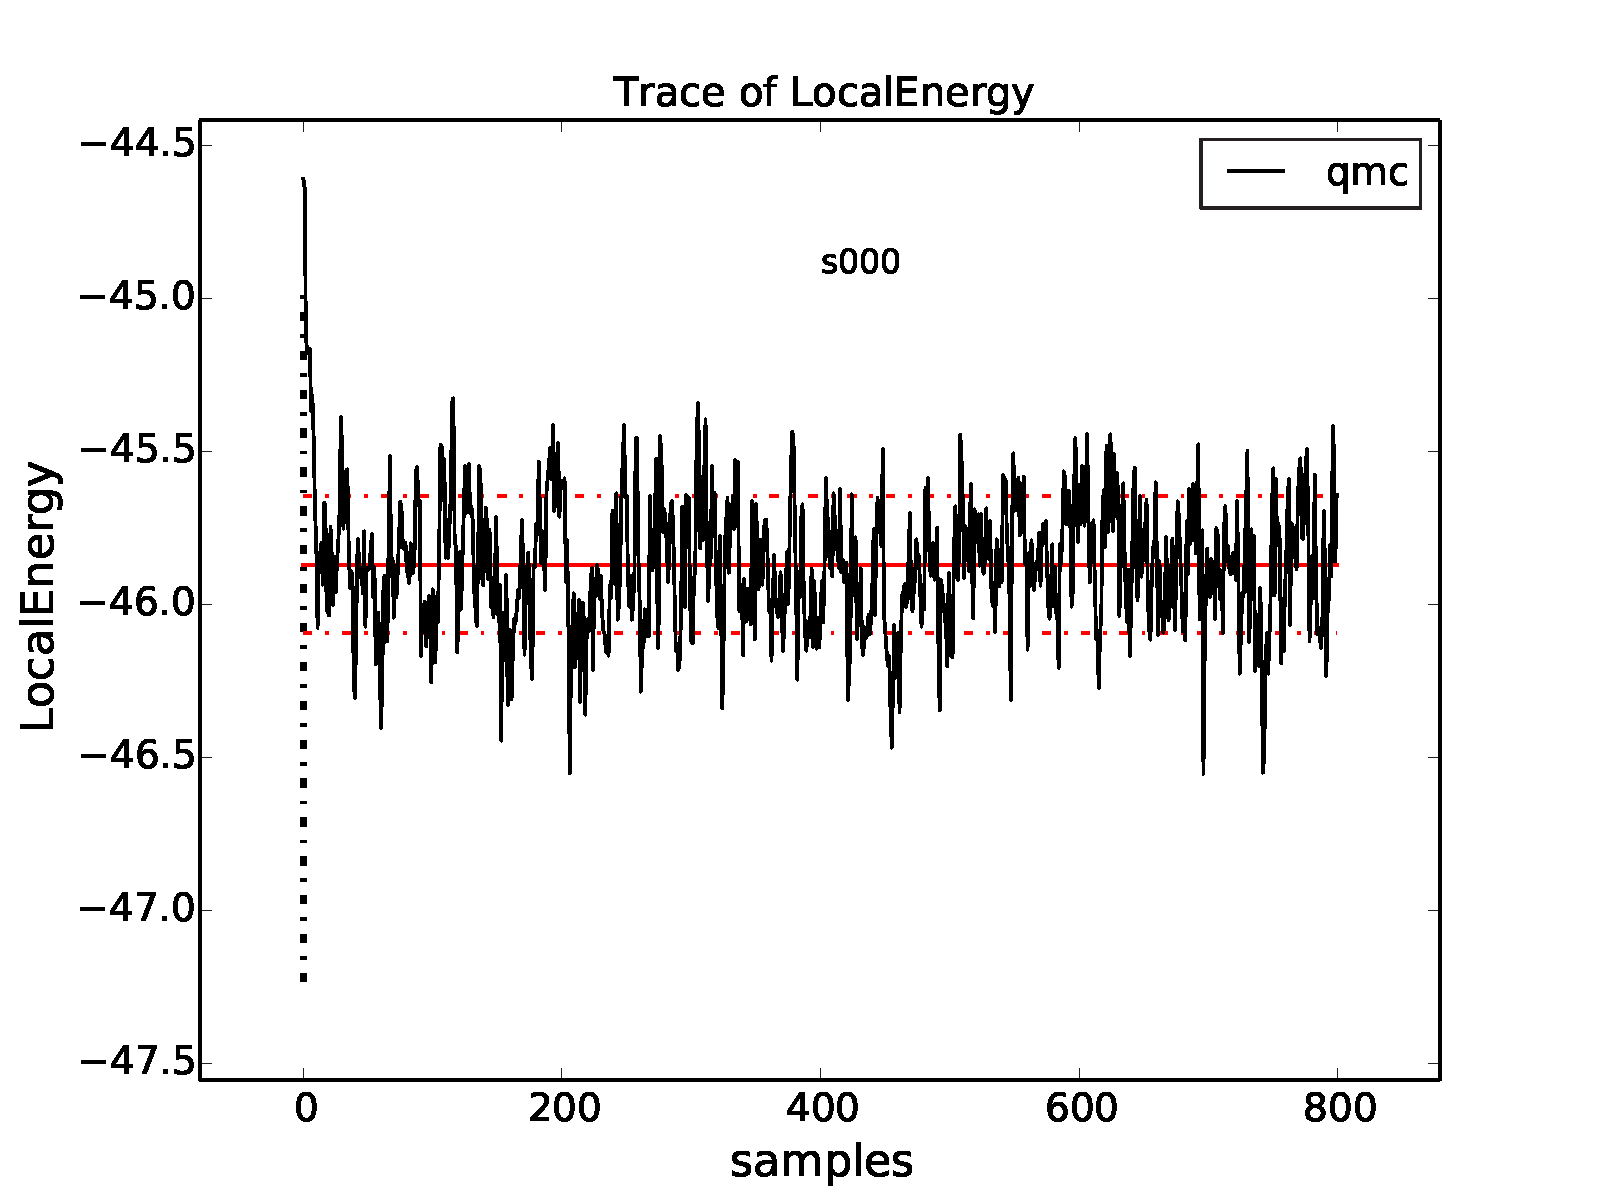
\includegraphics[trim = 0mm 0mm 0mm 0mm,clip,width=0.75\textwidth]{./figures/qmca_mean_error_trace.png}
\else
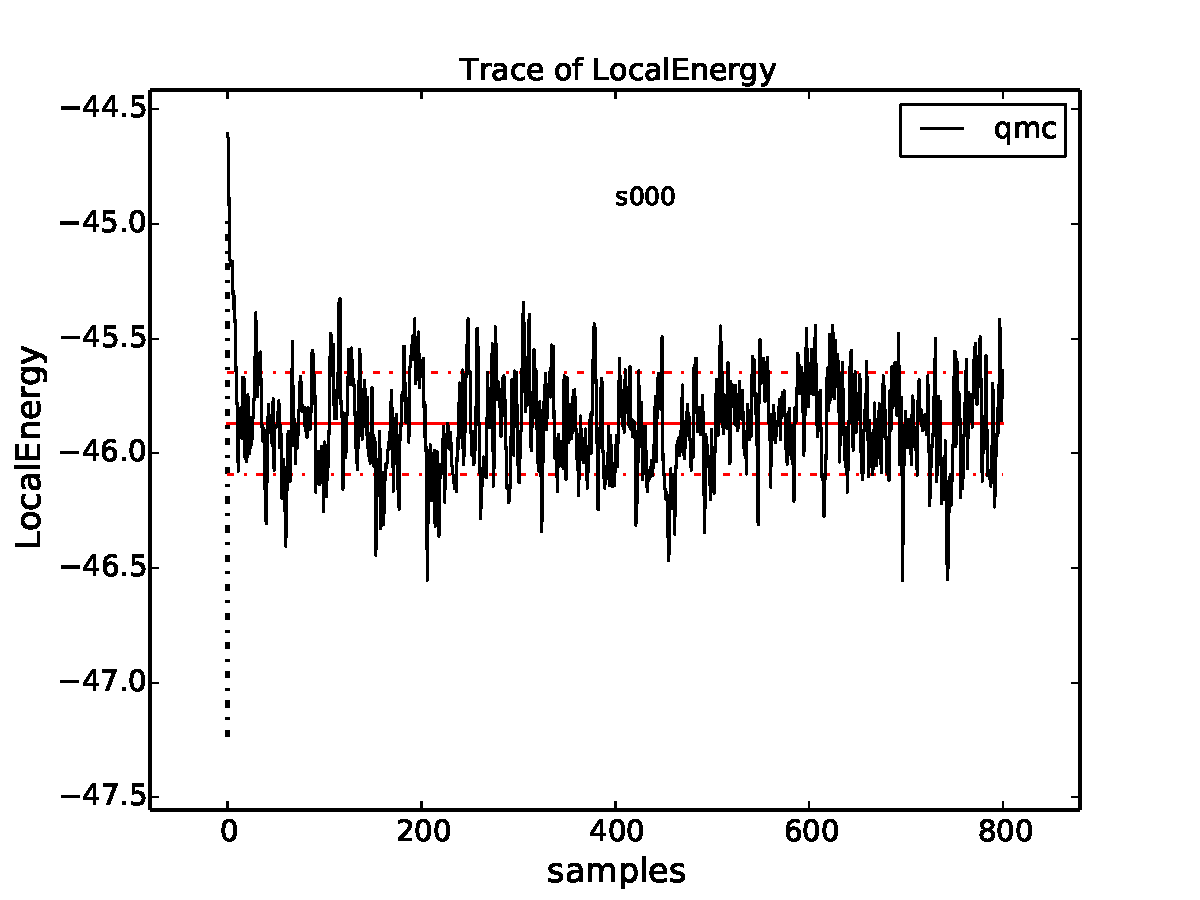
\includegraphics[trim = 0mm 0mm 0mm 0mm,clip,width=0.75\textwidth]{./figures/qmca_mean_error_trace.pdf}
\fi
\caption{Trace of the VMC local energy for an 8 atom cell of diamond generated with \texttt{qmca}.  The x-axis (``samples'') refers to the VMC block index in this case.}
\label{fig:qmca_mean_error_trace}
\end{center}
\end{figure}

If we exclude none of the equilibration data points, we get an 
erroneous estimate of $-45.870(2)$ Ha for the local energy:
\begin{shade}
>qmca -q e -e 0 qmc.s000.scalar.dat 
qmc  series 0  LocalEnergy           =  -45.870071 +/- 0.018072
\end{shade}
\noindent
The equilibration period is typically estimated by eye, though one should
check a few conservative values to ensure that the mean remains 
unaffected.  In this dataset, the equilibration appears to have been 
reached after 100 samples or so.  After excluding the first 100 
VMC blocks from the analysis we get:
\begin{shade}
>qmca -q e -e 100 qmc.s000.scalar.dat 
qmc  series 0  LocalEnergy           =  -45.877363 +/- 0.017432
\end{shade}
\noindent
This estimate ($-45.877(2)$ Ha) differs significantly from the 
$-45.870(2)$ Ha figure obtained from the full set of data, but it 
agrees with the rough estimate of $-45.876(2)$ Hartrees obtained 
with the abbreviated command (``\texttt{qmca -q e qmc.s000.scalar.dat}'').
This is because \texttt{qmca} makes a heuristic guess at the 
equilibration period and got it reasonably correct in this case. 
There are many cases where the heuristic guess fails and it should not 
be relied on for quality results.

We have so far obtained a statistically correct mean.  To obtain 
a statistically correct error bar it is best to include $\sim$100 or more 
statistically independent samples.  An estimate of the number 
of independent samples can be obtained by considering the 
autocorrelation time, which is essentially a measure of the number of 
samples that must be traversed before an uncorrelated/independent sample 
is reached.  We can get an estimate of the autocorrelation time 
in the following way:
\begin{shade}
>qmca -q e -e 100 qmc.s000.scalar.dat --sac
qmc  series 0  LocalEnergy           =  -45.877363 +/- 0.017432    4.8 
\end{shade}
\noindent
The flag ``\texttt{--sac}'' stands for (s)how (a)uto(c)orrelation.  
In this case the autocorrelation estimate is $4.8\approx 5$ samples. 
Since the total run contained 800 samples and we have excluded 100 of 
them, we can estimate the number of independent samples as 
$(800-100)/5=140$.  In this case, the error bar is expected to be 
estimated reasonably well.

Please keep in mind that the error bar represents the expected range
of the mean with a certainty of only $\sim 70\%$, i.e. it is a one
sigma error bar.  The actual mean value will lie outside the range
indicated by the error bar in one out of every three runs and in a set
of 20 runs one value can be expected to deviate from its estimate by
twice the error bar.


\subsection{Judging wavefunction optimization}
\label{sec:qmca_judge_opt}
Wavefunction optimization is a highly non-linear and sometimes 
sensitive process.  As such, there is a risk that systematic 
errors encountered at this stage of the QMC process can be propagated 
into subsequent (expensive) DMC runs unless they are guarded against 
with vigilance.

In this section we again consider an 8 atom cell of diamond, but 
now in the context of Jastrow optimization (one- and two-body terms). 
In optimization runs it is often preferable to use a large number 
of \texttt{warmupsteps} ($\sim 100$) so that equilibration bias does 
not propagate into the optimization process.  We can check that 
the added warmup has had its intended effect by again checking the 
local energy trace:
\begin{shade}
>qmca -t -q e *scalar*
\end{shade}
\noindent
The resulting plot can be found in Fig. \ref{fig:qmca_judge_opt}. 
In this case sufficient \texttt{warmupsteps} were used to exit 
the equilibration period before samples were collected and we can 
proceed without using the ``\texttt{-e}'' option with \texttt{qmca}.

\begin{figure}
\begin{center}
\ifdefined\HCode  
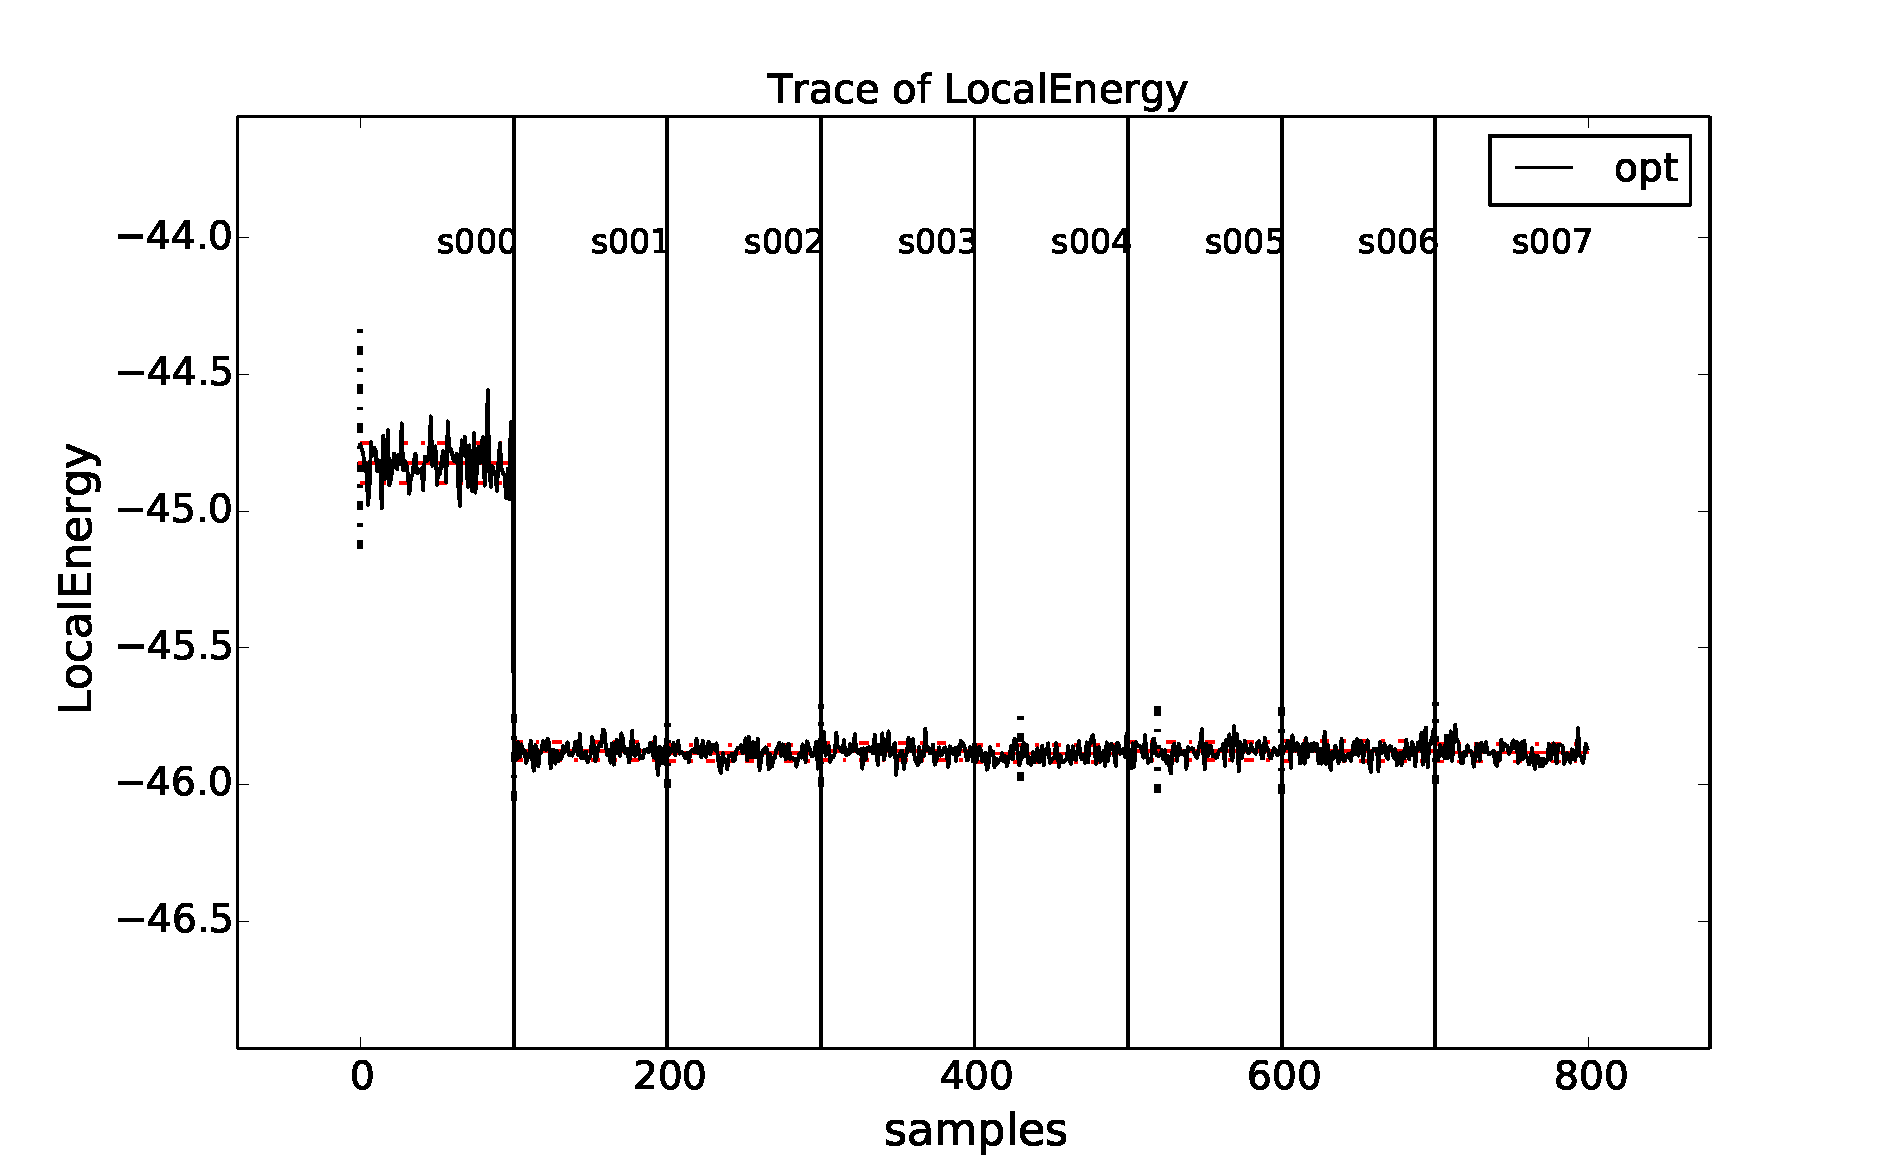
\includegraphics[trim = 0mm 0mm 0mm 0mm, clip,width=0.9\textwidth]{./figures/qmca_judge_opt.png}
\else
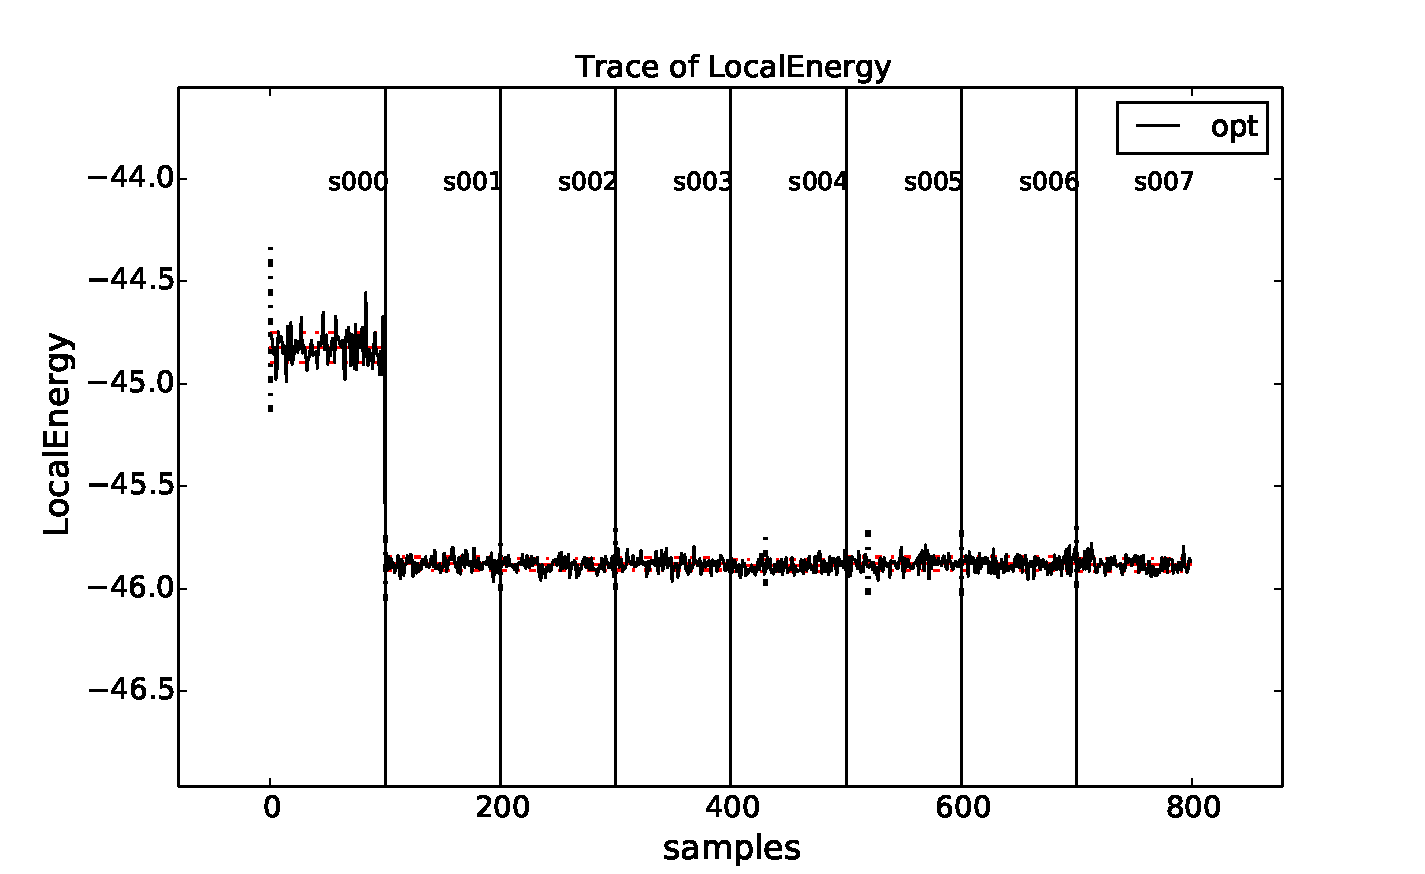
\includegraphics[trim = 0mm 0mm 0mm 0mm, clip,width=0.9\columnwidth]{./figures/qmca_judge_opt.pdf}
\fi
\end{center}
\caption{Trace of the local energy during one- and two-body Jastrow optimization for an 8 atom cell of diamond generated with \texttt{qmca}.  Data for each optimization cycle (QMCPACK series) is separated by a vertical black line.
}
\label{fig:qmca_judge_opt}
\end{figure}

After inspecting the trace, we should inspect the text output 
from \texttt{qmca}, now including the total energy and its variance:
\begin{shade}
>qmca -q ev opt*scalar.dat
                            LocalEnergy               Variance           ratio 
opt  series 0  -44.823616 +/- 0.007430   7.054219 +/- 0.041998   0.1574 
opt  series 1  -45.877643 +/- 0.003329   1.095362 +/- 0.041154   0.0239 
opt  series 2  -45.883191 +/- 0.004149   1.077942 +/- 0.021555   0.0235 
opt  series 3  -45.877524 +/- 0.003094   1.074047 +/- 0.010491   0.0234 
opt  series 4  -45.886062 +/- 0.003750   1.061707 +/- 0.014459   0.0231 
opt  series 5  -45.877668 +/- 0.003475   1.091585 +/- 0.021637   0.0238 
opt  series 6  -45.877109 +/- 0.003586   1.069205 +/- 0.009387   0.0233 
opt  series 7  -45.882563 +/- 0.004324   1.058771 +/- 0.008651   0.0231 
\end{shade}
\noindent
The flags ``\texttt{-q ev}'' requested the energy (\texttt{e}) and 
the variance (\texttt{v}).  For this combination of quantities, a 
third column (``\texttt{ratio}'') is printed containing the ratio 
of the variance and the absolute value of the local energy.
The variance/energy ratio is an intensive quantity and is useful  
to inspect regardless of the system under study.  Successful 
optimization of molecules and solids of any size generally result 
in comparable values for the variance/energy ratio. 

The first line of 
the output (``\texttt{series 0}'') corresponds to the local energy 
and variance of the system without a Jastrow factor (all Jastrow 
coefficients were initialized to zero in this case), reflecting the 
quality of the orbitals alone. For pseudopotential systems, a 
variance/energy ratio $>0.20$ Ha generally indicates there is a problem 
with the input orbitals that needs to be resolved prior to 
performing wavefunction optimization.  

The subsequent lines correspond to energies and variances of 
intermediate parameterizations of the trial wavefunction during 
the optimization process.  The output line containing 
``\texttt{opt  series 1}'', for example, corresponds to the trial 
wavefunction parameterized during the ``\texttt{series 0}'' step 
(the parameters of this wavefunction would be found in an output 
file matching \texttt{*s000*opt.xml}).  The first thing to check 
about the resulting optimization is again the variance/energy ratio. 
For pseudopotential systems, a variance/energy ratio $<0.03$ Ha is 
consistent with a trial wavefunction of production quality, and values 
of $0.01$ Ha are rarely obtainable for standard Slater-Jastrow 
wavefunctions.  By this metric, all parameterizations obtained for 
optimizations performed in series 0-6 are of comparable quality 
(note that the quality of the wavefunction obtained during optimization 
series 7 is effectively unknown).

A good way to further discriminate among the parameterizations is to 
plot the energy and variance as a function of series with \texttt{qmca}:
\begin{shade}
>qmca -p -q ev opt*scalar.dat
\end{shade}
\noindent
The ``\texttt{-p}'' option results in plots of means plus error bars 
vs. series for all requested quantities.
The resulting plots for the local energy and variance are shown 
in Fig. \ref{fig:qmca_opt_ev}.  In this case the resulting energies 
and variances are statistically indistinguishable for all optimization 
cycles.  

\begin{figure}
  \centering
  \parbox{0.47\linewidth}{%
    \ifdefined\HCode
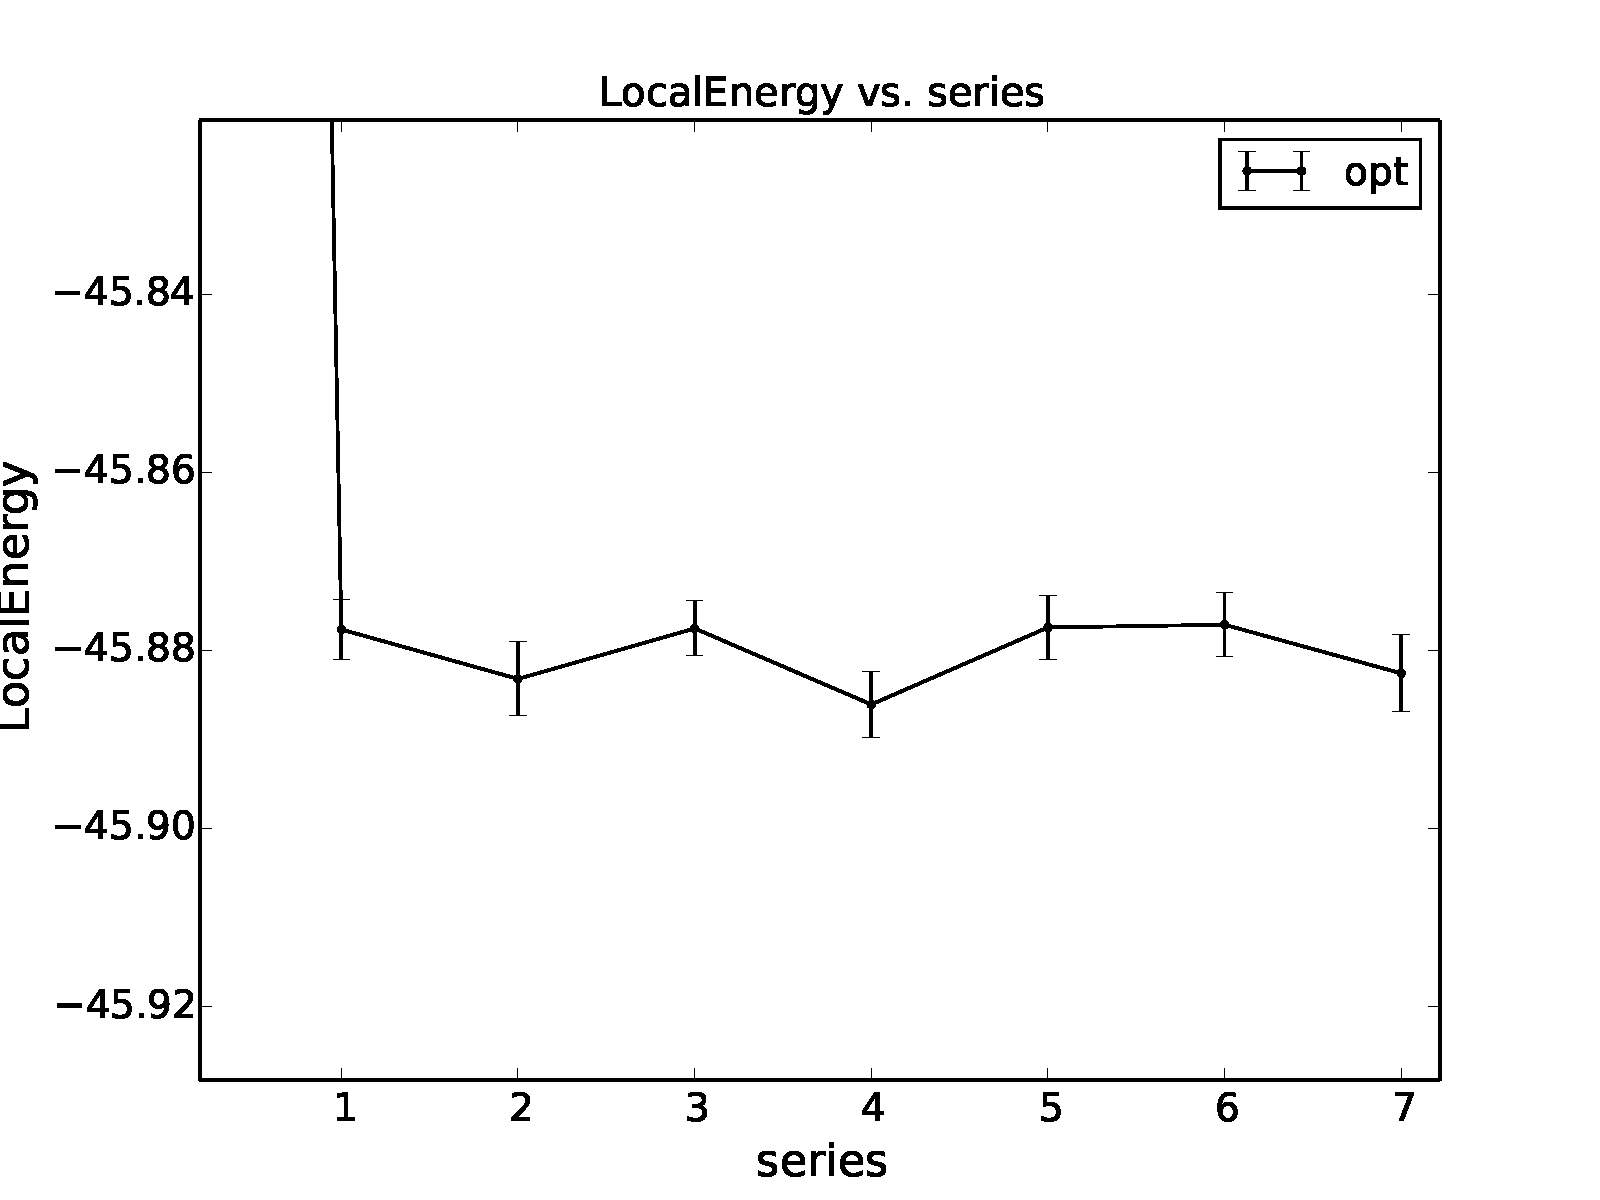
\includegraphics[trim=0mm 0mm 4mm 0mm,clip,width=\linewidth]{./figures/qmca_opt_energy.png}
\else
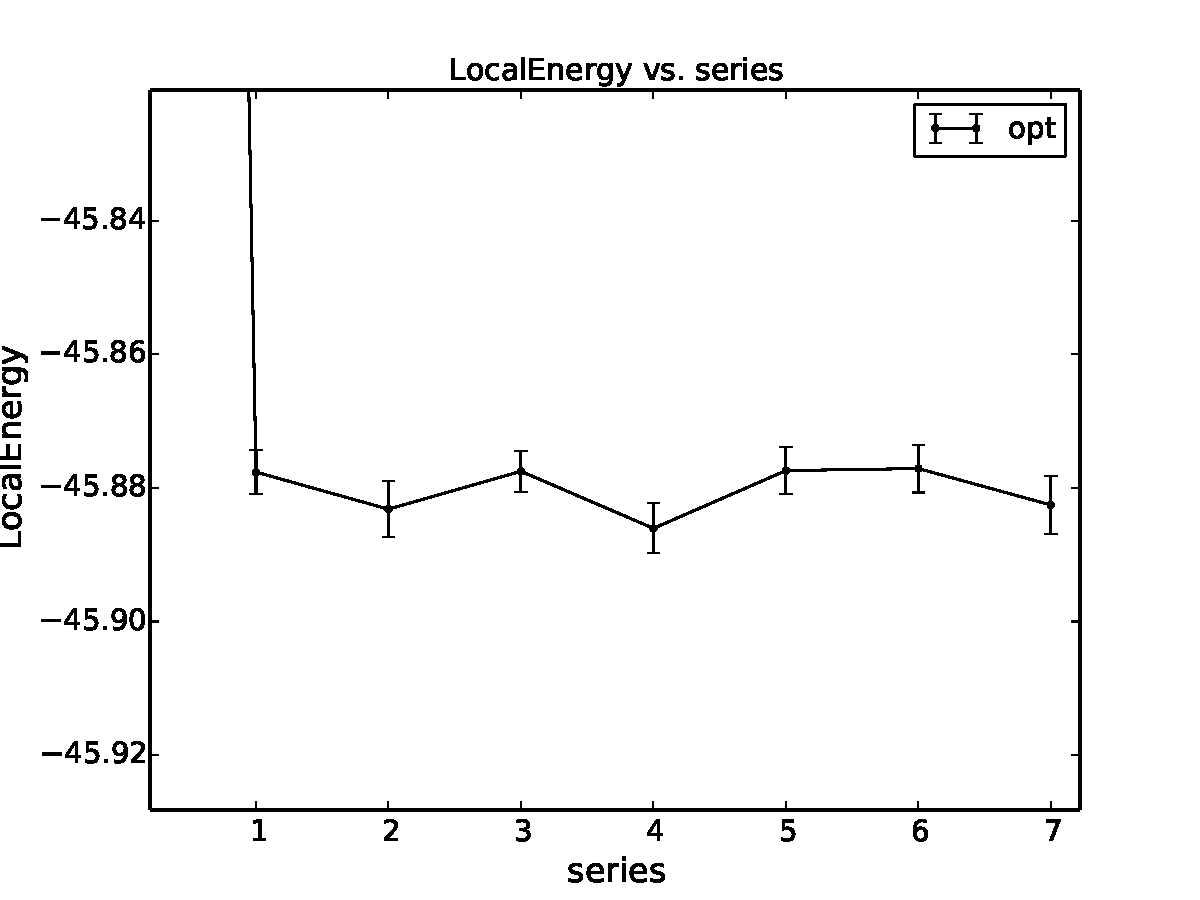
\includegraphics[trim=0mm 0mm 4mm 0mm,clip,width=\linewidth]{./figures/qmca_opt_energy.pdf}
\fi%
  }%
  \qquad\begin{minipage}{0.47\linewidth}%
   \ifdefined\HCode
   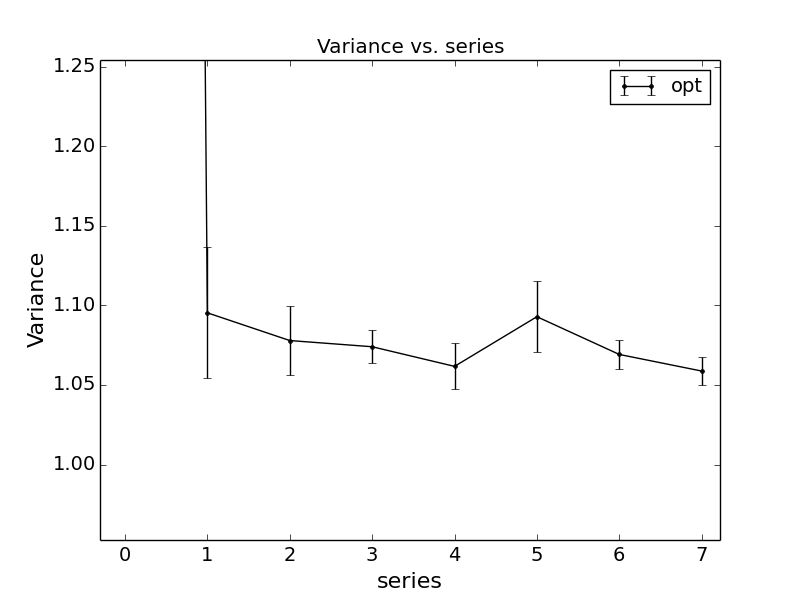
\includegraphics[trim=0mm 0mm 4mm 0mm,clip,width=\linewidth]{./figures/qmca_opt_variance.png}
    \else
    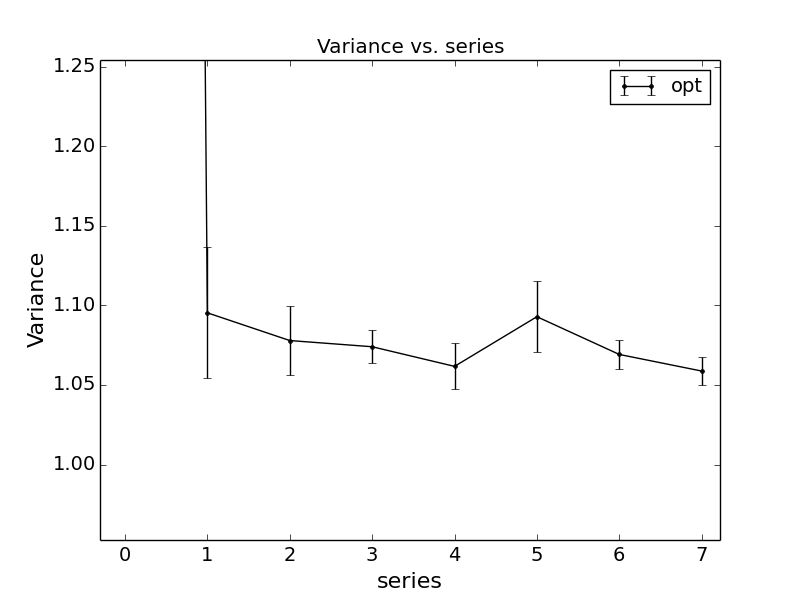
\includegraphics[trim=0mm 0mm 4mm 0mm,clip,width=\linewidth]{./figures/qmca_opt_variance.png}
\fi%
  \end{minipage}%
  \caption{Energy and variance vs. optimization series for an 8 atom cell of diamond as plotted by \texttt{qmca}.}%
  \label{fig:qmca_opt_ev}%
\end{figure}

A good way to choose the optimal wavefunction for use in DMC is to select 
the one with lowest statistically significant energy within the set of 
optimized wavefunctions with reasonable variance (\emph{e.g.} among 
those with variance/energy ratio $<0.03$ Ha).  For pseudopotential 
calculations, minimizing according to the total energy is recommended 
to reduce locality errors in DMC.


\subsection{Judging diffusion Monte Carlo runs}
\label{sec:qmca_judge_dmc}
Judging the quality of the DMC projection process requires more 
care than this needed in VMC.  In order to reduce bias, a small 
timestep is required in the approximate projector but this also 
leads to slow equilibration and long autocorrelation times.  
Systematic errors in the projection process can also arise from 
statistical fluctuations due to pseudopotentials or from trial 
wavefunctions with larger than necessary variance.

\begin{figure}
\begin{center}
  \ifdefined\HCode  
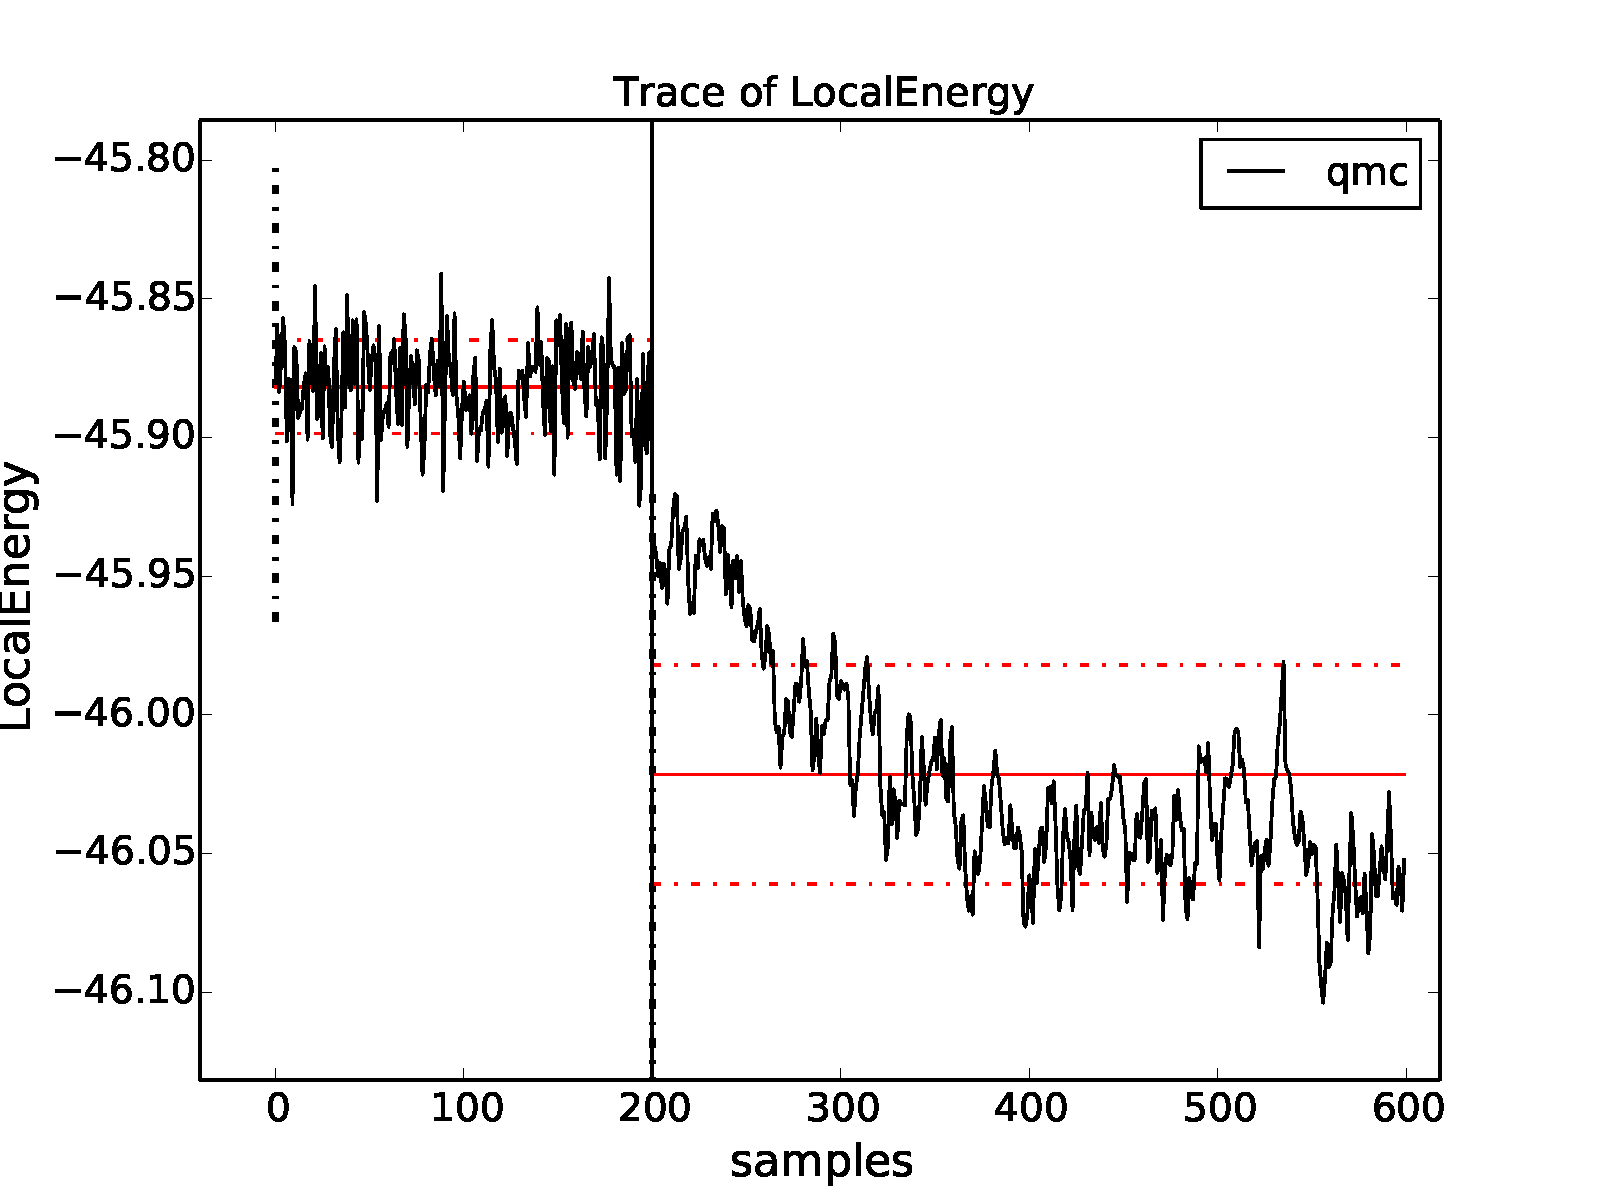
\includegraphics[trim = 0mm 0mm 0mm 0mm,clip,width=0.75\columnwidth]{./figures/qmca_short_dmc.png}
\else
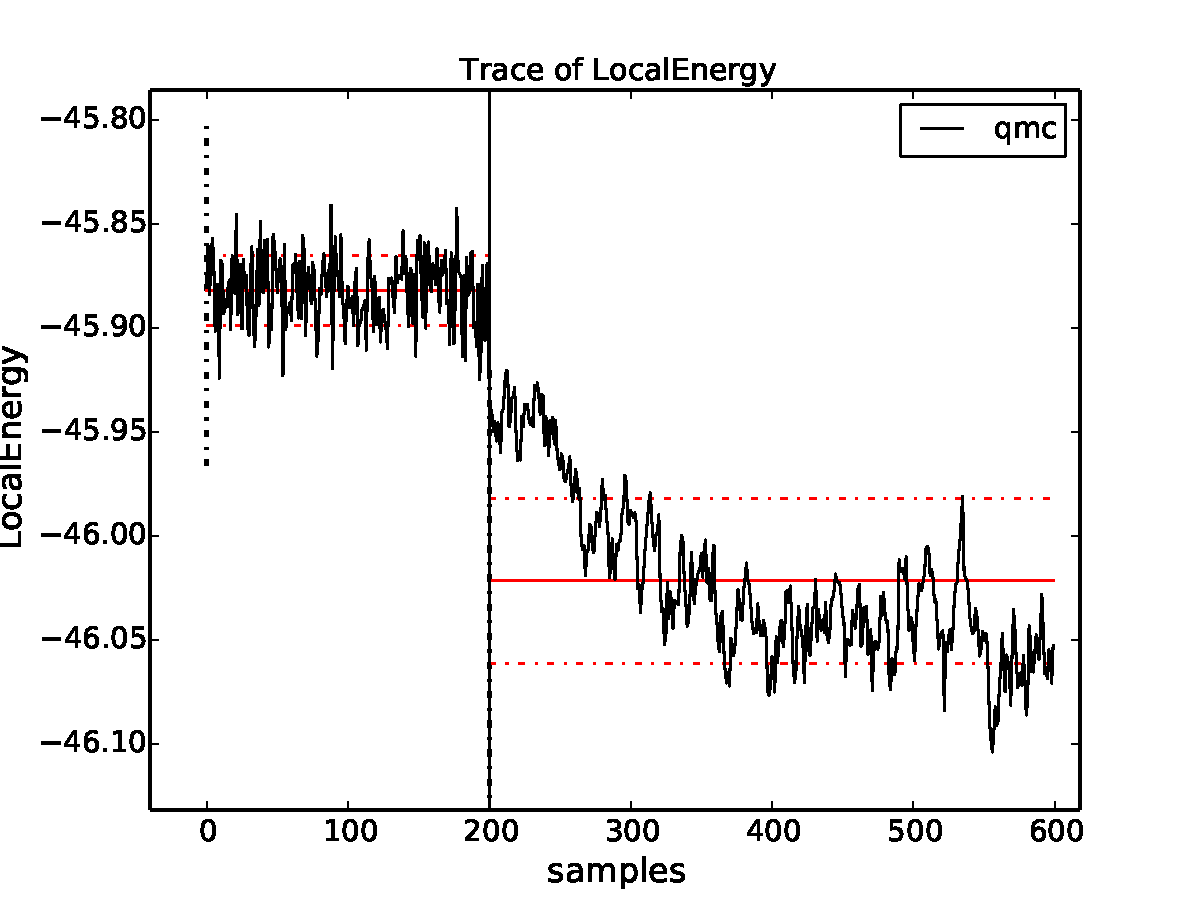
\includegraphics[trim = 0mm 0mm 0mm 0mm,clip,width=0.75\columnwidth]{./figures/qmca_short_dmc.pdf}
\fi
\end{center}
\caption{Trace of the local energy for VMC followed by DMC with a small timestep ($0.002$ Ha$^{-1}$) for an 8 atom cell of diamond generated with \texttt{qmca}.}
\label{fig:qmca_short_dmc}
\end{figure}

To illustrate the problems that can arise with respect to slow 
equilibration and long autocorrelation times, we consider the 
8 atom diamond system with VMC ($200$ blocks of $160$ steps) followed 
by DMC ($400$ blocks of $5$ steps) with a small timestep ($0.002$ Ha$^{-1}$).
A good first step in assessing the quality of any DMC run is 
to plot the trace of the local energy:
\begin{shade}
>qmca -t -q e -e 0 *scalar*
\end{shade}
\noindent
The resulting trace plot is shown in Fig. \ref{fig:qmca_short_dmc}.  
As always, the DMC local energy decreases exponentially away from 
the VMC value but in this case it takes a long time to do so.  
At least half of the DMC run is inefficiently consumed by equilibration.
If we are not careful to inspect and remove the transient, the estimated 
DMC energy will be strongly biased by the transient as shown by the 
horizontal red line (estimated mean) in the figure.  The autocorrelation 
time is also large ($\sim 12$ blocks):
\begin{shade}
>qmca -q e -e 200 --sac *s001.scalar*
qmc  series 1  LocalEnergy           =  -46.045720 +/- 0.004813   11.6
\end{shade}
\noindent
Of the included 200 blocks, fewer than 20 contribute to the estimated error 
bar, indicating that we cannot trust the reported error bar.  
This can also be demonstrated directly from the data.  If we halve the number 
of samples included to 100, we would expect from Gaussian statistics 
that the error bar would grow by a factor of $\sqrt{2}$, but instead we 
get
\begin{shade}
>qmca -q e -e 300 *s001.scalar*
qmc  series 1  LocalEnergy           =  -46.048537 +/- 0.009280
\end{shade}
\noindent
which erroneously shows an estimated increase in the error bar by a factor 
of about two.  Overall this run is simply too short to gain meaningful 
information.  

Consider the case where we are interested in the cohesive energy of 
diamond and, after having performed a timestep study of the cohesive 
energy, we have found that the energy difference between bulk diamond 
and atomic carbon converges to our required accuracy with a larger 
timestep of $0.01$ Ha$^{-1}$.  In a production setting, a small cell 
could be used to determine  the appropriate timestep while a larger 
cell would subsequently be used to obtain a converged cohesive energy, 
though for purposes of demonstration we still proceed with the 8 atom 
cell here.  The new timestep of $0.01$ Ha$^{-1}$ will result in a shorter 
autocorrelation time than the smaller timestep used previously, but 
we would like to shorten the equilibration time further still.  This 
can be achieved by using a larger timestep (say $0.02$ Ha$^{-1}$) in a 
short intermediate DMC run used to walk down the transient.  The 
rapidly achieved equilibrium with the $0.02$ Ha$^{-1}$ timestep 
projector will be much nearer to the $0.01$ Ha$^{-1}$ timestep one 
we seek than the original VMC equilibrium, and so we can expect 
a shortened secondary equilibration time in the production 
$0.01$ Ha$^{-1}$ timestep run. Note that this procedure is fully 
general, even if one has to deal with an even shorter 
timestep--\emph{e.g.} $0.002$ Ha$^{-1}$--for a particular problem.

\begin{figure}
\begin{center}
\ifdefined\HCode  
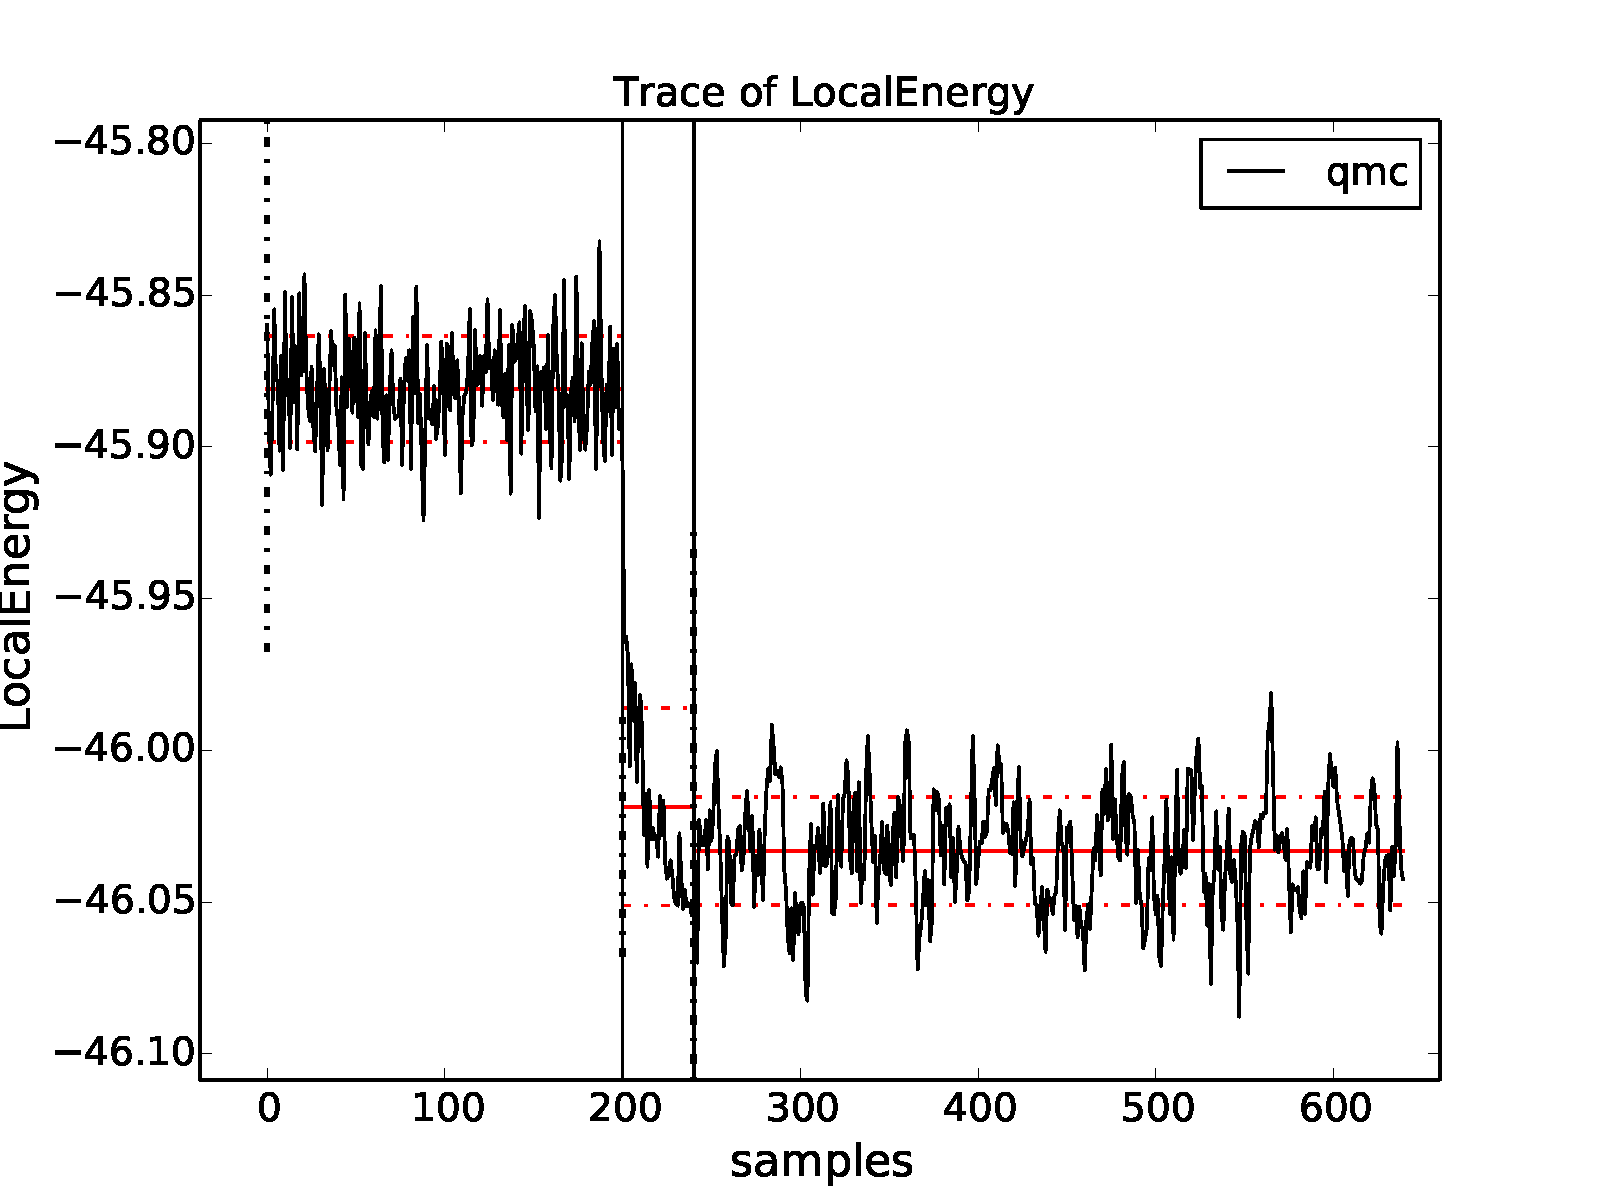
\includegraphics[trim = 0mm 0mm 0mm 0mm, clip,width=0.75\columnwidth]{./figures/qmca_accel_dmc.png}
\else
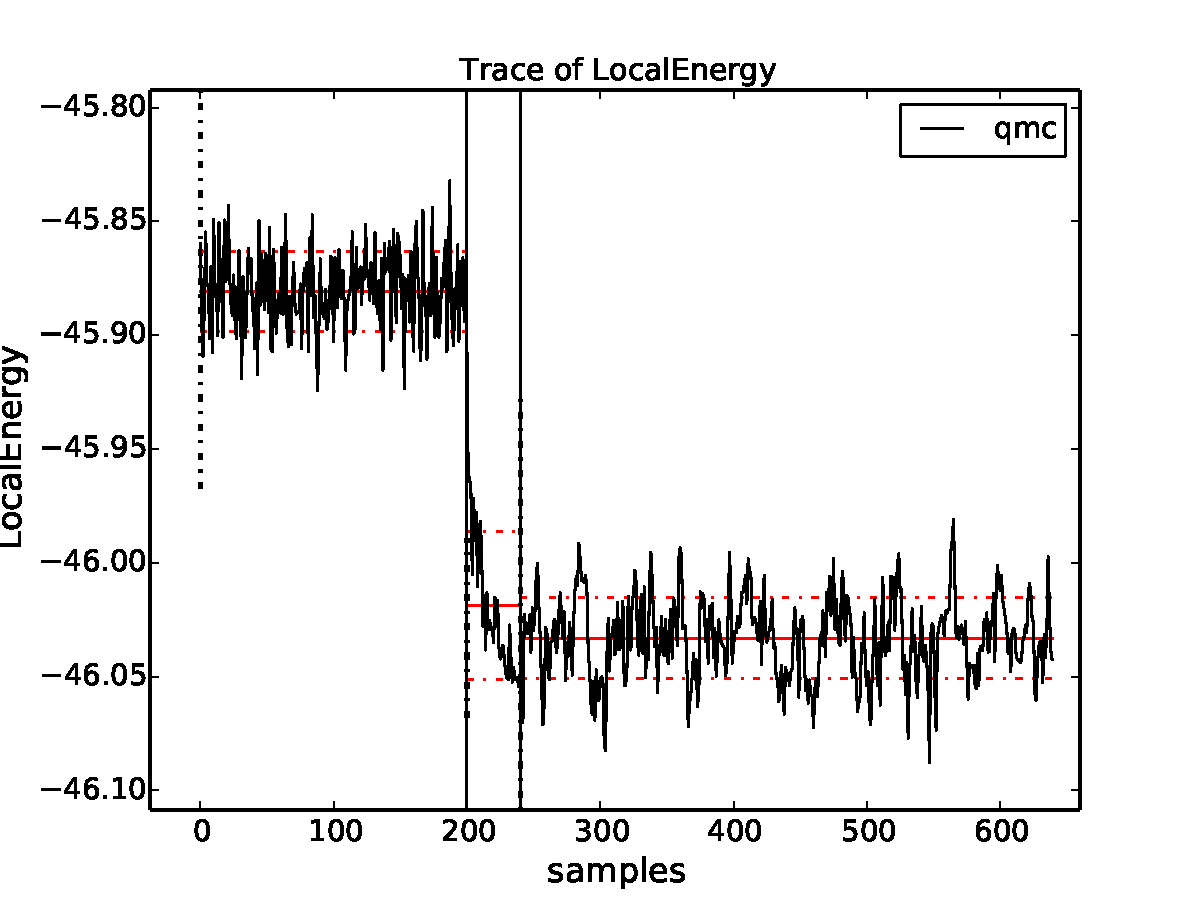
\includegraphics[trim = 0mm 0mm 0mm 0mm, clip,width=0.75\columnwidth]{./figures/qmca_accel_dmc.pdf}
\fi
\end{center}
\caption{Trace of the local energy for VMC followed by a short intermediate DMC with a large timestep ($0.02$ Ha$^{-1}$) and finally a production DMC run with a timestep of $0.01$ Ha$^{-1}$.  Calculations were performed in an 8 atom cell of diamond.} 
\label{fig:qmca_accel_dmc}
\end{figure}

We now rerun the prior example but with an intermediate DMC 
calculation using $40$ blocks of $5$ steps with a timestep of 
$0.02$ Ha$^{-1}$ followed by a production DMC calculation 
using $400$ blocks of $10$ steps with a timestep of $0.01$ Ha$^{-1}$.
We again plot the local energy trace using \texttt{qmca}
\begin{shade}
>qmca -t -q e -e 0 *scalar*
\end{shade}
\noindent
with the result shown in Fig. \ref{fig:qmca_accel_dmc}.
The projection transient has been effectively contained in the 
short DMC run with a larger timestep.  As expected, the 
production run contains only a short equilibration period.
Removing the first 20 blocks as a precaution, we obtain an estimate 
of the total energy in VMC and DMC:
\begin{shade}
>qmca -q ev -e 20 --sac qmc.*.scalar.dat 
                            LocalEnergy               Variance           ratio 
qmc  series 0  -45.881042 +/- 0.001283    1.0   1.076726 +/- 0.007013    1.0   0.0235 
qmc  series 1  -46.040814 +/- 0.005046    3.9   1.011303 +/- 0.016807    1.1   0.0220 
qmc  series 2  -46.032960 +/- 0.002077    5.2   1.014940 +/- 0.002547    1.0   0.0220 
\end{shade}
\noindent
Notice that the variance energy ratio in DMC ($0.220$ Ha) is similar to, but 
slightly smaller than, what is obtained with VMC ($0.235$ Ha).  If the DMC 
variance/energy ratio is ever significantly larger than in VMC, this is 
cause to be concerned about the correctness of the DMC run.  Also notice 
the estimated autocorrelation time ($\sim 5$ blocks).  This leaves us with 
an estimated $\sim 76$ independent samples, though we should recall that 
the autocorrelation time is also a statistical estimate which can be improved 
with more data.  We can gain a better estimate of the autocorrelation 
time by using the \texttt{*.dmc.dat} files which contain output data resolved 
per step rather than per block (there are $10\times$ more steps than blocks 
in this example case):
\begin{shade}
>qmca -q ev -e 200 --sac qmc.s002.dmc.dat 
                            LocalEnergy               Variance           ratio 
qmc  series 2  -46.032909 +/- 0.002068   31.2   1.015781 +/- 0.002536    1.4   0.0221 
\end{shade}
\noindent
This results in an estimated autocorrelation time of $\sim 31$ steps, or 
$\sim 3$ blocks, indicating that we actually have $\sim 122$ independent 
samples which should be sufficient to obtain a trustworthy error bar.
Our final DMC total energy is estimated to be $-46.0329(2)$ Ha.

\begin{figure}
\begin{center}
  \ifdefined\HCode
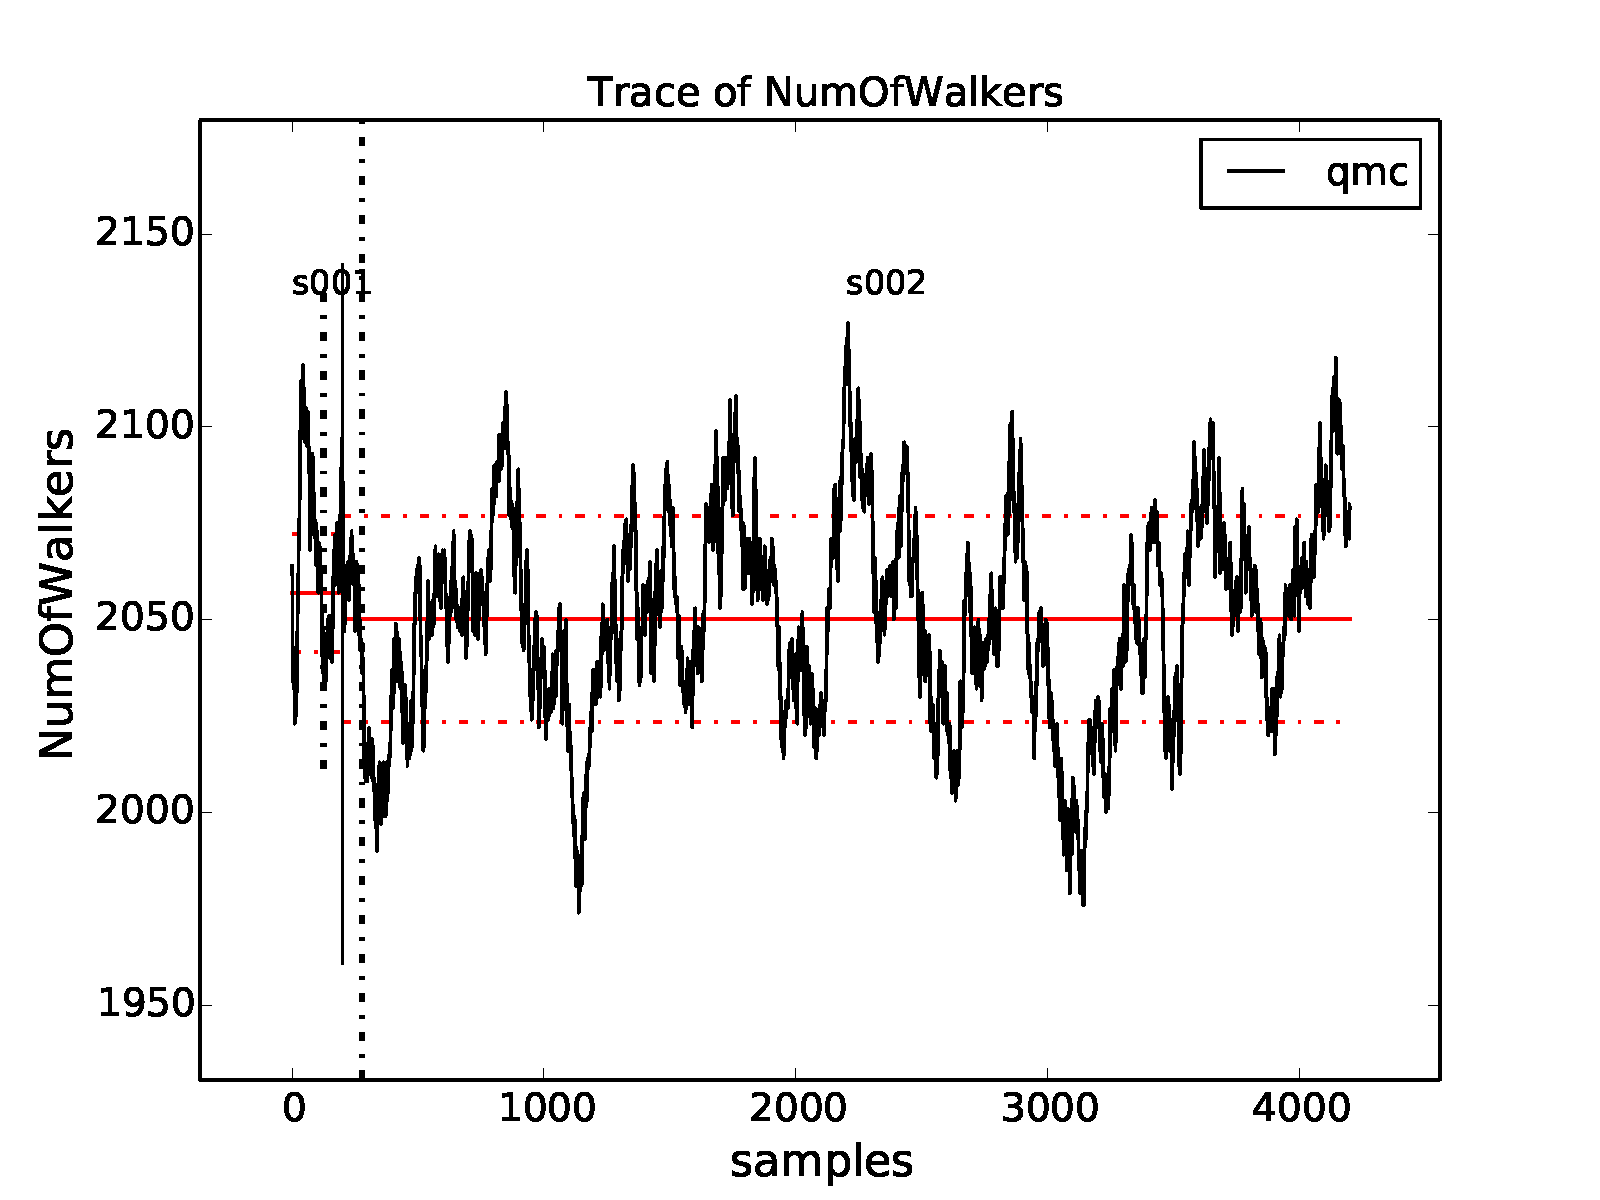
\includegraphics[trim = 0mm 0mm 0mm 0mm, clip,width=0.75\columnwidth]{./figures/qmca_pop_trace.png}
\else
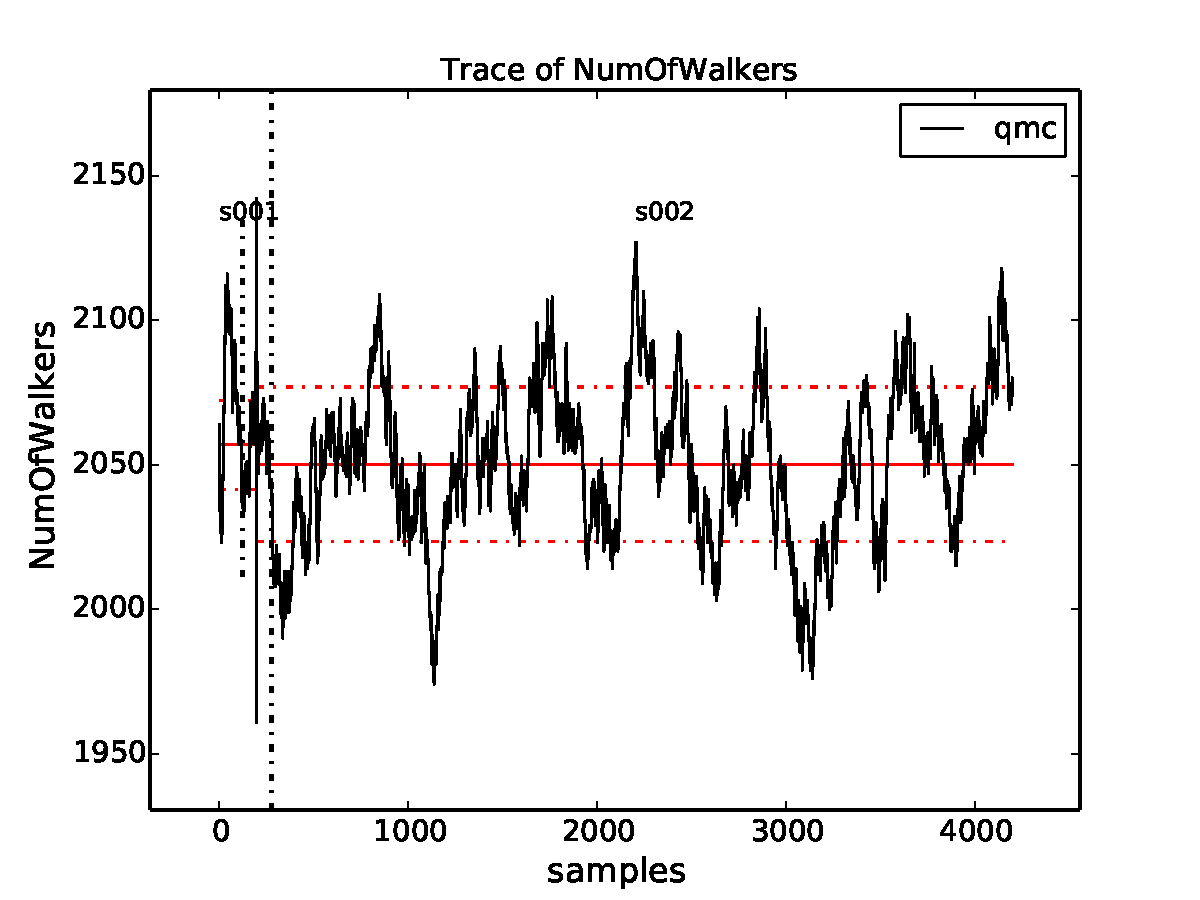
\includegraphics[trim = 0mm 0mm 0mm 0mm, clip,width=0.75\columnwidth]{./figures/qmca_pop_trace.pdf}
\fi
\end{center}
\caption{Trace of the DMC walker population for an 8 atom cell of diamond obtained with \texttt{qmca}.}
\label{fig:qmca_pop_trace}
\end{figure}

Another simulation property that should be explicitly monitored  
is the behavior of the DMC walker population.  Data regarding the 
walker population is contained in the \texttt{*.dmc.dat} files.
In Fig. \ref{fig:qmca_pop_trace} we show the trace of the DMC 
walker population for the current run:
\begin{shade}
>qmca -t -q nw *dmc.dat
qmc  series 1  NumOfWalkers          =  2056.905405 +/- 8.775527 
qmc  series 2  NumOfWalkers          =  2050.164160 +/- 4.954850 
\end{shade}
\noindent
Following a DMC run the walker population should be checked for 
two qualities: 1) that the population is sufficiently large (a number 
$>2000$ is generally sufficient to reduce population control bias) and  
2) that the population fluctuates benignly around its intended target 
value. In this case the target walker count (provided in the input file)
was $2048$ and we can confirm from the plot that the population is simply 
fluctuating around this value.  Also from the text output we have a dynamic 
population estimate of 2050(5) walkers.  Rapid population reductions or 
increases--population explosions--are indicative of problems with a run.  
These issues sometimes result from using a considerably poor wavefunction 
(see comments regarding variance/energy ratio above and in the preceding 
subsections).  QMCPACK has internal guards in place that prevent 
the population from exceeding certain maximum and minimum bounds, so 
in particularly faulty runs one might see the population ``stabilize'' 
to a constant value much larger or smaller than the target.  In these 
cases the cause(s) for the divergent population behavior need to 
be investigated and resolved before proceeding further.



\subsection{Obtaining other quantities}
\label{sec:qmca_other_quantities}
A number of other scalar valued quantities are available with 
\texttt{qmca}.  To obtain text output for all quantities 
available, simply exclude the ``\texttt{-q}'' option used in 
the prior examples.  Below is example output for a DMC calculation 
of the 8 atom diamond system from the \texttt{scalar.dat} file:
\begin{shade}
>qmca -e 20 qmc.s002.scalar.dat 
qmc  series 2 
  LocalEnergy           =          -46.0330 +/-           0.0021 
  Variance              =            1.0149 +/-           0.0025 
  Kinetic               =            33.851 +/-            0.019 
  LocalPotential        =           -79.884 +/-            0.020 
  ElecElec              =          -11.4483 +/-           0.0083 
  LocalECP              =           -22.615 +/-            0.029 
  NonLocalECP           =            5.2815 +/-           0.0079 
  IonIon                =            -51.10 +/-             0.00 
  LocalEnergy_sq        =           2120.05 +/-             0.19 
  BlockWeight           =          20514.27 +/-            48.38 
  BlockCPU              =            1.4890 +/-           0.0038 
  AcceptRatio           =         0.9963954 +/-        0.0000055 
  Efficiency            =             71.88 +/-             0.00 
  TotalTime             =            565.80 +/-             0.00 
  TotalSamples          =           7795421 +/-                0 
\end{shade}
\noindent
Similarly, for the \texttt{dmc.dat} file we get
\begin{shade}
>qmca -e 20 qmc.s002.dmc.dat 
qmc  series 2 
  LocalEnergy           =          -46.0329 +/-           0.0020 
  Variance              =            1.0162 +/-           0.0025 
  TotalSamples          =           8201275 +/-                0 
  TrialEnergy           =          -46.0343 +/-           0.0023 
  DiffEff               =         0.9939150 +/-        0.0000088 
  Weight                =           2050.23 +/-             4.82 
  NumOfWalkers          =              2050 +/-                5 
  LivingFraction        =          0.996427 +/-         0.000021 
  AvgSentWalkers        =            0.2625 +/-           0.0011 
\end{shade}

Any subset of desired quantities can be obtained by using the 
``\texttt{-q}'' option with either the full names of the quantities 
listed above 
\begin{shade}
>qmca -q 'LocalEnergy Kinetic LocalPotential' -e 20 qmc.s002.scalar.dat 
qmc  series 2 
  LocalEnergy           =          -46.0330 +/-           0.0021 
  Kinetic               =            33.851 +/-            0.019 
  LocalPotential        =           -79.884 +/-            0.020 
\end{shade}
\noindent
or with their corresponding abbreviations
\begin{shade}
>qmca -q ekp -e 20 qmc.s002.scalar.dat 
qmc  series 2 
  LocalEnergy           =          -46.0330 +/-           0.0021 
  Kinetic               =            33.851 +/-            0.019 
  LocalPotential        =           -79.884 +/-            0.020 
\end{shade}
\noindent
Abbreviations for each quantity can be found by typing \texttt{qmca}
at the command line with no other input.  A current list is provided 
below:
\begin{shade}
  Abbreviations and full names for quantities:
    ar              = AcceptRatio
    bc              = BlockCPU
    bw              = BlockWeight
    ce              = CorrectedEnergy
    de              = DiffEff
    e               = LocalEnergy
    ee              = ElecElec
    eff             = Efficiency
    ii              = IonIon
    k               = Kinetic
    kc              = KEcorr
    l               = LocalECP
    le2             = LocalEnergy_sq
    mpc             = MPC
    n               = NonLocalECP
    nw              = NumOfWalkers
    p               = LocalPotential
    sw              = AvgSentWalkers
    te              = TrialEnergy
    ts              = TotalSamples
    tt              = TotalTime
    v               = Variance
    w               = Weight
\end{shade}
\noindent
Please see the output overview for \texttt{scalar.dat} 
(Sec. \ref{sec:scalardat_file}) and \texttt{dmc.dat} 
(Sec. \ref{sec:dmc_file}) for more information about 
these quantities.  The data analysis aspects for these 
quantities is essentially the same as for the local 
energy as covered in the preceding subsections. 
Quantities that do not belong to an equilibrium distribution 
(\emph{e.g.} \texttt{BlockCPU}) are somewhat different, though they 
still exhibit statistical fluctuations.


\subsection{Processing multiple files}
\label{sec:qmca_multiple_files}
Batch file processing is a common use case for \texttt{qmca}. 
If we consider an ``equation of state'' calculation involving 
the 8 atom diamond cell we have used so far, we might be interested 
in the total energy for the various supercell volumes along the 
trajectory from compression to expansion.  After checking 
the traces (``\texttt{qmca -t -q e scale\_*/vmc/*scalar*}'') 
to settle on a sensible equilibration cutoff as discussed in 
the preceding subsections we can obtain the total energies 
all at once:
\begin{shade}
>qmca -q ev -e 40 scale_*/vmc/*scalar*
                            LocalEnergy               Variance           ratio 
scale_0.80/vmc/qmc  series 0 -44.670984 +/- 0.006051  2.542384 +/- 0.019902  0.0569 
scale_0.82/vmc/qmc  series 0 -44.982818 +/- 0.005757  2.413011 +/- 0.022626  0.0536 
scale_0.84/vmc/qmc  series 0 -45.228257 +/- 0.005374  2.258577 +/- 0.019322  0.0499 
scale_0.86/vmc/qmc  series 0 -45.415842 +/- 0.005532  2.204980 +/- 0.052978  0.0486 
scale_0.88/vmc/qmc  series 0 -45.570215 +/- 0.004651  2.061374 +/- 0.014359  0.0452 
scale_0.90/vmc/qmc  series 0 -45.683684 +/- 0.005009  1.988539 +/- 0.018267  0.0435 
scale_0.92/vmc/qmc  series 0 -45.751359 +/- 0.004928  1.913282 +/- 0.013998  0.0418 
scale_0.94/vmc/qmc  series 0 -45.791622 +/- 0.005026  1.843704 +/- 0.014460  0.0403 
scale_0.96/vmc/qmc  series 0 -45.809256 +/- 0.005053  1.829103 +/- 0.014536  0.0399 
scale_0.98/vmc/qmc  series 0 -45.806235 +/- 0.004963  1.775391 +/- 0.015199  0.0388 
scale_1.00/vmc/qmc  series 0 -45.783481 +/- 0.005293  1.726869 +/- 0.012001  0.0377 
scale_1.02/vmc/qmc  series 0 -45.741655 +/- 0.005627  1.681776 +/- 0.011496  0.0368 
scale_1.04/vmc/qmc  series 0 -45.685101 +/- 0.005353  1.682608 +/- 0.015423  0.0368 
scale_1.06/vmc/qmc  series 0 -45.615164 +/- 0.005978  1.652155 +/- 0.010945  0.0362 
scale_1.08/vmc/qmc  series 0 -45.543037 +/- 0.005191  1.646375 +/- 0.013446  0.0361 
scale_1.10/vmc/qmc  series 0 -45.450976 +/- 0.004794  1.707649 +/- 0.048186  0.0376 
scale_1.12/vmc/qmc  series 0 -45.371851 +/- 0.005103  1.686997 +/- 0.035920  0.0372 
scale_1.14/vmc/qmc  series 0 -45.265490 +/- 0.005311  1.631614 +/- 0.012381  0.0360 
scale_1.16/vmc/qmc  series 0 -45.161961 +/- 0.004868  1.656586 +/- 0.014788  0.0367 
scale_1.18/vmc/qmc  series 0 -45.062579 +/- 0.005971  1.671998 +/- 0.019942  0.0371 
scale_1.20/vmc/qmc  series 0 -44.960477 +/- 0.004888  1.651864 +/- 0.009756  0.0367 
\end{shade}
\noindent

In this case, we are using a Jastrow factor optimized only at the 
equilibrium geometry (``\texttt{scale\_1.00}'') but with radial 
cutoffs restricted to the Wigner-Seitz radius of the most compressed 
supercell (``\texttt{scale\_0.80}'') to avoid introducing wavefunction 
cusps at the cell boundary (QMCPACK would have aborted with a warning in 
this case, had we tried).  It is clear that this restricted Jastrow factor 
is not an optimal choice as it yields variance/energy ratios between $0.036$ 
and $0.057$ Ha.  This issue is largely a result of our undersized (8 atom) 
supercell and larger cells should always be used in real production 
calculations.

Batch processing is also possible for multiple quantities.  If multiple 
quantities are requested, an additional line is inserted to separate 
results from different runs:
\begin{shade}
>qmca -q 'e bc eff' -e 40 scale_*/vmc/*scalar*
scale_0.80/vmc/qmc  series 0 
  LocalEnergy           =          -44.6710 +/-           0.0061 
  BlockCPU              =           0.02986 +/-          0.00038 
  Efficiency            =          38104.00 +/-             0.00 

scale_0.82/vmc/qmc  series 0 
  LocalEnergy           =          -44.9828 +/-           0.0058 
  BlockCPU              =           0.02826 +/-          0.00013 
  Efficiency            =          44483.91 +/-             0.00 

scale_0.84/vmc/qmc  series 0 
  LocalEnergy           =          -45.2283 +/-           0.0054 
  BlockCPU              =           0.02747 +/-          0.00030 
  Efficiency            =          52525.12 +/-             0.00 

scale_0.86/vmc/qmc  series 0 
  LocalEnergy           =          -45.4158 +/-           0.0055 
  BlockCPU              =           0.02679 +/-          0.00013 
  Efficiency            =          50811.55 +/-             0.00 

scale_0.88/vmc/qmc  series 0 
  LocalEnergy           =          -45.5702 +/-           0.0047 
  BlockCPU              =           0.02598 +/-          0.00015 
  Efficiency            =          74148.79 +/-             0.00 

scale_0.90/vmc/qmc  series 0 
  LocalEnergy           =          -45.6837 +/-           0.0050 
  BlockCPU              =           0.02527 +/-          0.00011 
  Efficiency            =          65714.98 +/-             0.00 

...
\end{shade}



\subsection{Twist averaging}
\label{sec:qmca_twist_average}
Twist averaging can be performed straightforwardly for any 
output quantity listed in Sec. \ref{sec:qmca_other_quantities} 
with \texttt{qmca}.  We illustrate these capabilities by 
repeating the 8 atom diamond DMC runs performed in Sec. 
\ref{sec:qmca_judge_dmc} at eight real valued supercell twist 
angles (a $2\times 2\times 2$ Monkhorst-Pack grid centered at 
the $\Gamma$-point).  Data traces for each twist can be overlapped 
on the same plot:
\begin{shade}
>qmca -to -q e -e '30 20 30' *scalar* --legend outside
\end{shade}
\noindent
The ``\texttt{-o}'' option requests the plots be overlapped; 
eight separate plots would be generated otherwise.  The 
equilibration input ``\texttt{-e '30 20 30'}'' cuts out from 
the analyzed data the first 30 blocks for series 0 (VMC), 
20 blocks for series 1 (intermediate DMC), and 30 blocks for 
series 2 (production DMC).  The resulting plot is shown in 
Fig. \ref{fig:qmca_twist_overlap}

\begin{figure}
\begin{center}
\ifdefined\HCode
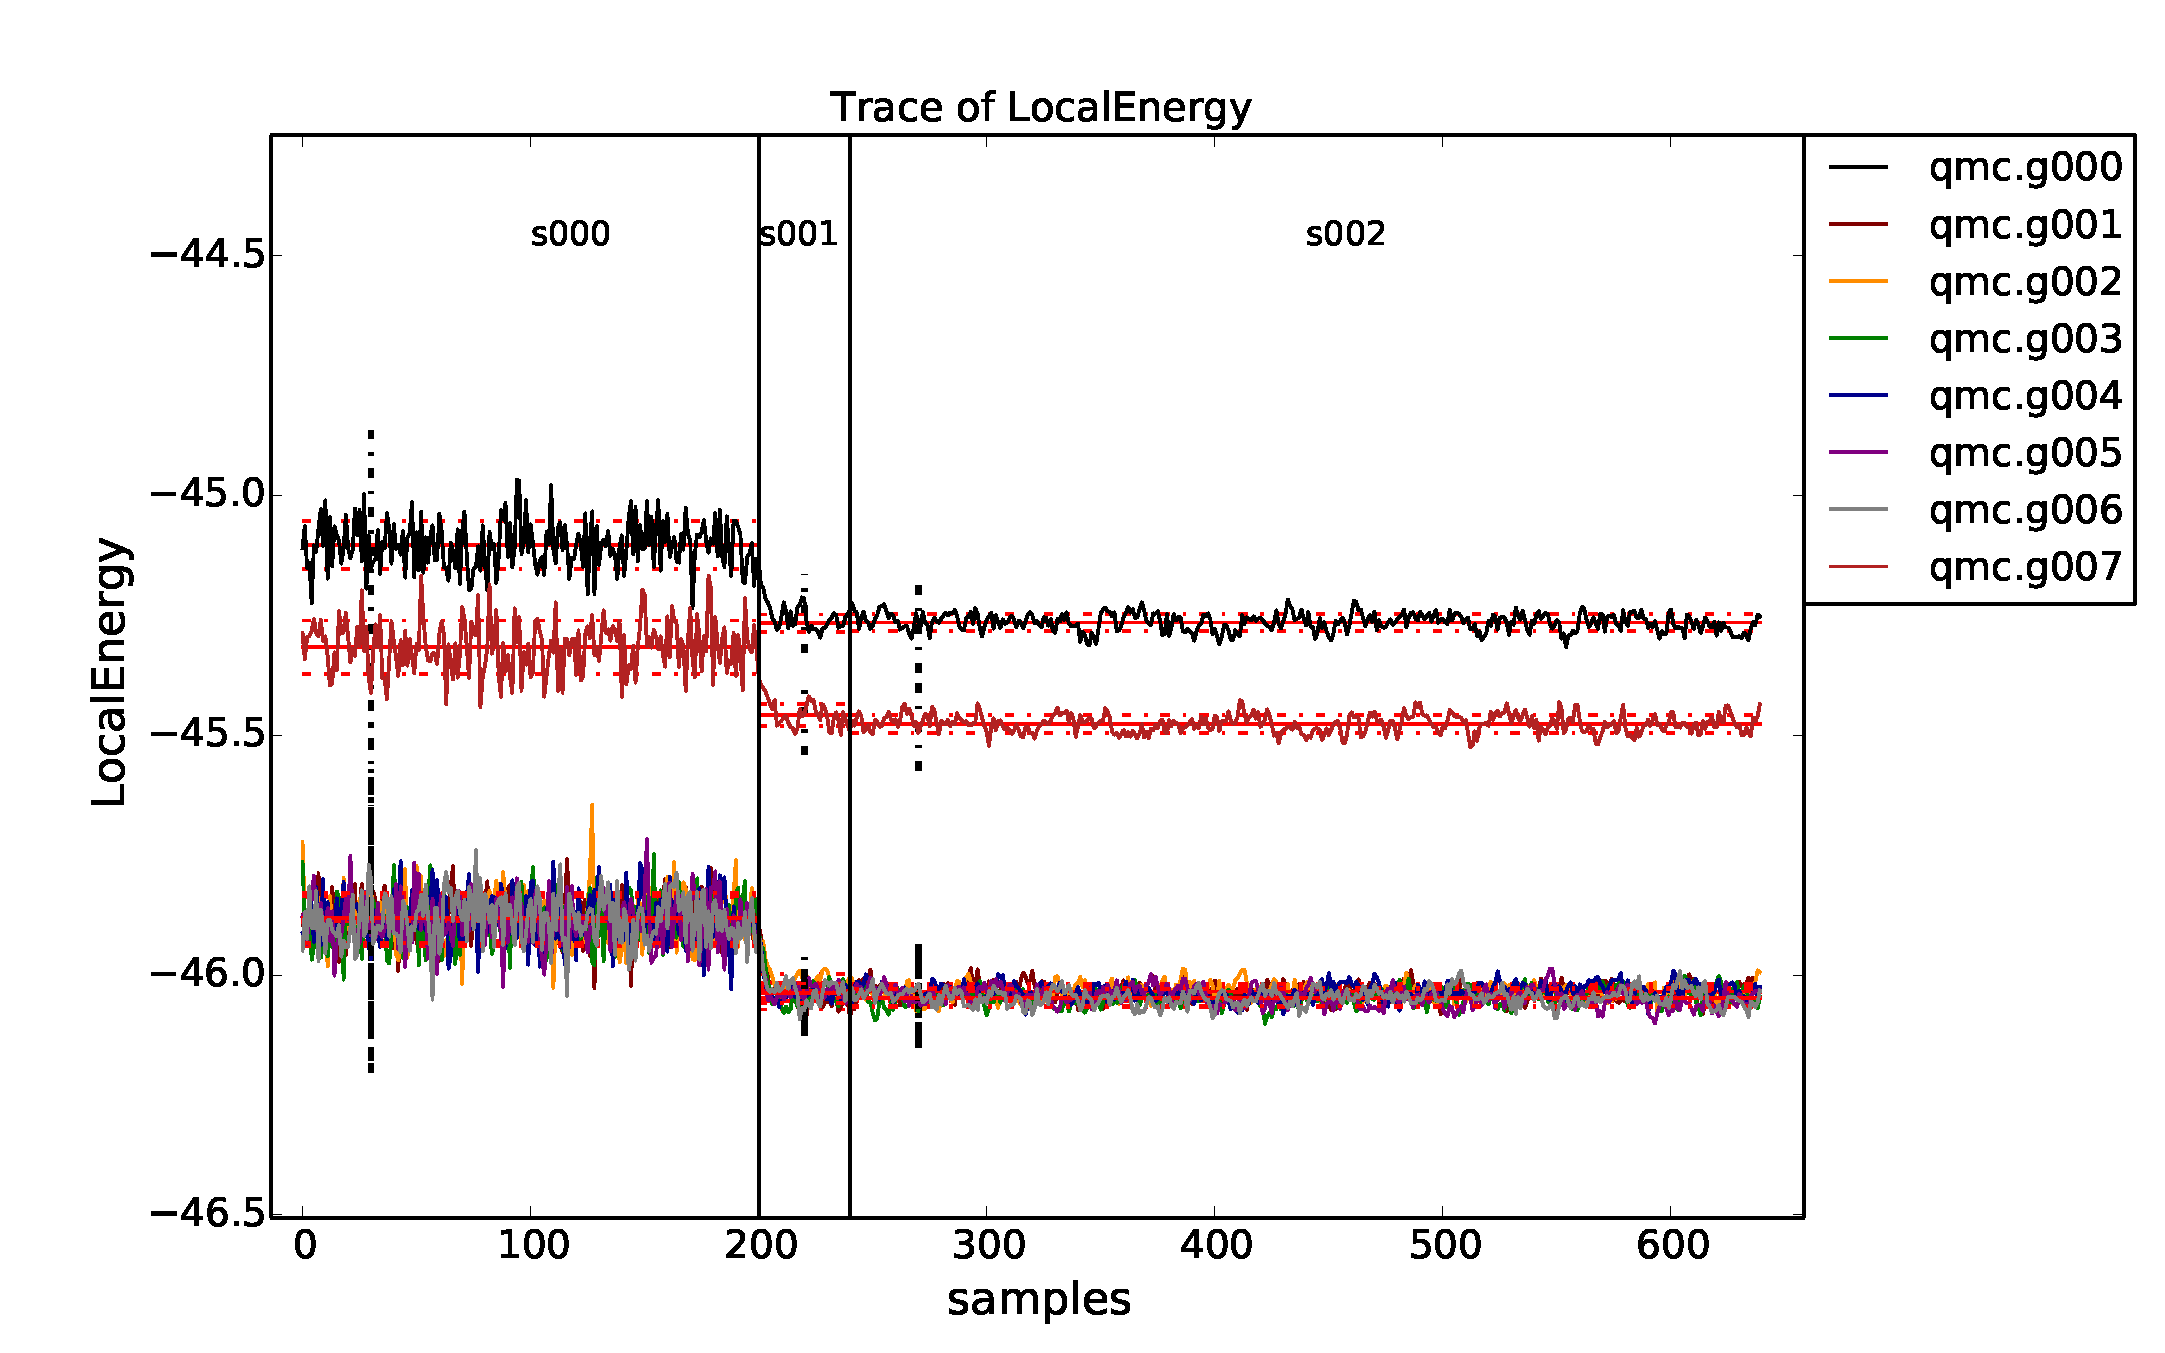
\includegraphics[trim = 0mm 0mm 0mm 0mm, clip,width=0.9\columnwidth]{./figures/qmca_twist_trace_overlap.png}
\else
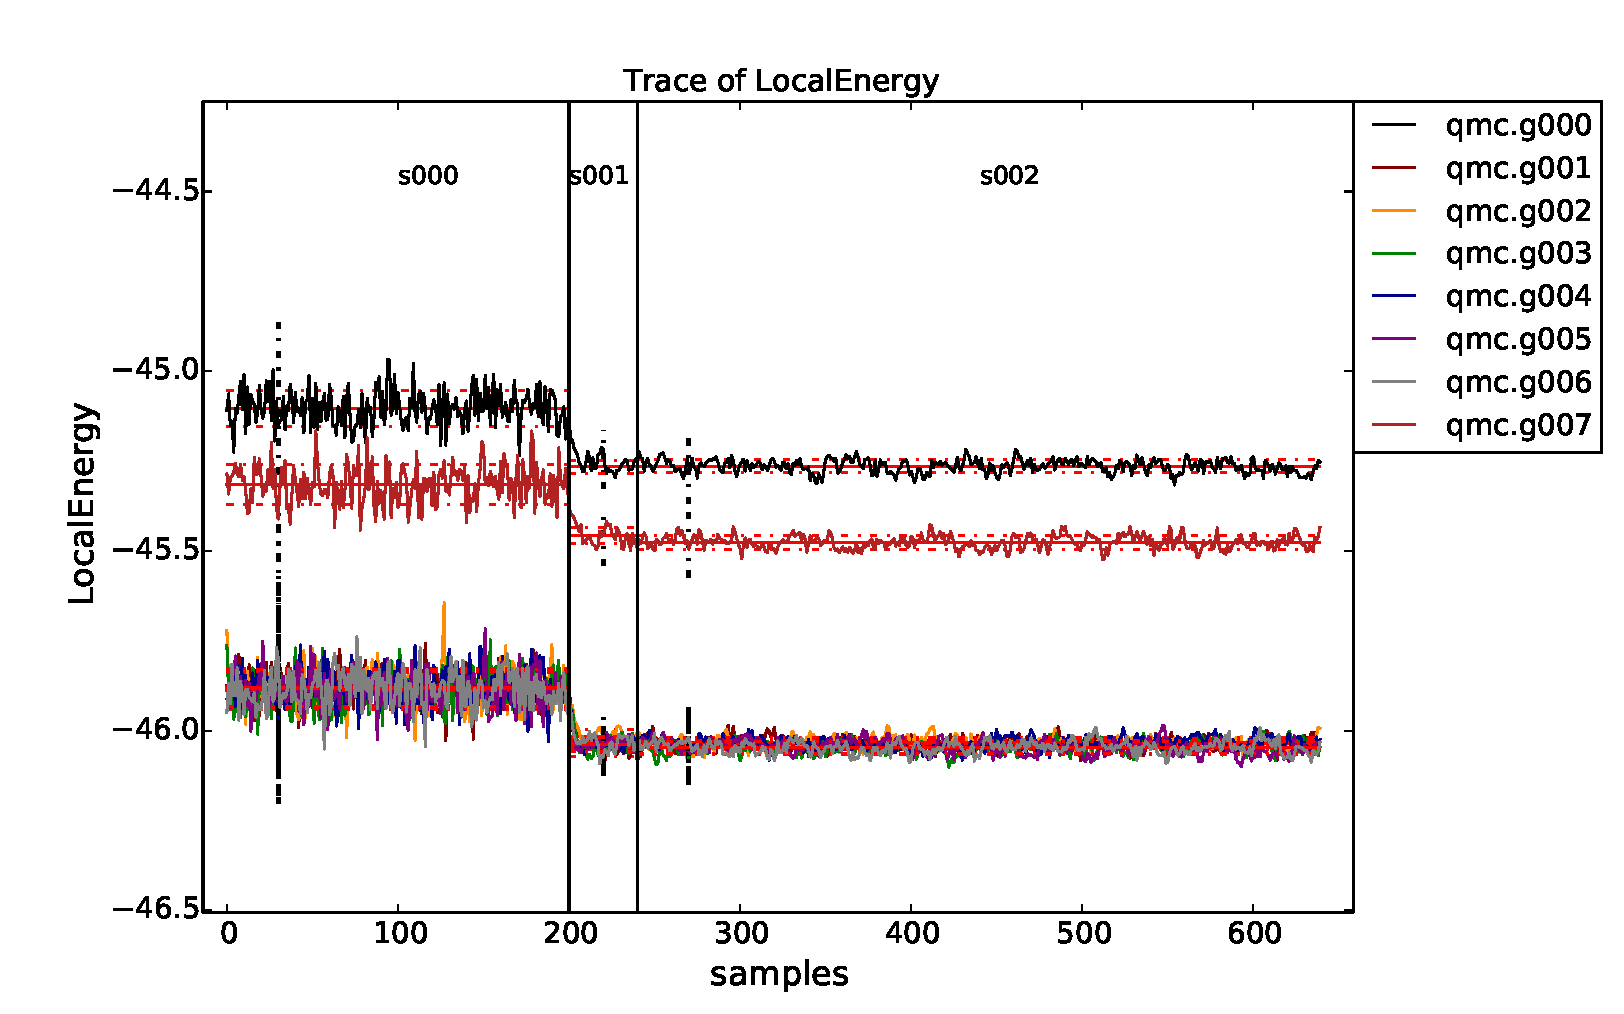
\includegraphics[trim = 0mm 0mm 0mm 0mm, clip,width=0.9\columnwidth]{./figures/qmca_twist_trace_overlap.pdf}
\fi
\end{center}
\caption{Overlapped energy traces from VMC to DMC for an 8 supercell of diamond obtained with \texttt{qmca}.  Data for each twist appears in a different color.}
\label{fig:qmca_twist_overlap}
\end{figure}

Twist averaging is performed by providing the ``\texttt{-a}'' 
option.  If provided on its own, uniform weights are applied 
to each twist angle.  To obtain a trace plot with twist averaging 
enforced, use a command similar to the following:
\begin{shade}
>qmca -a -t -q e -e '30 20 30' *scalar*
\end{shade}
\noindent
The resulting plot is shown in Fig. \ref{fig:qmca_twist_average}.
As can be seen from the trace plot, the chosen equilibration lengths 
are appropriate and we proceed to obtain the twist averaged total energy
from the \texttt{scalar.dat} files
\begin{shade}
>qmca -a -q ev -e 30 --sac *s002.scalar*
                            LocalEnergy               Variance           ratio 
avg  series 2  -45.873369 +/- 0.000753    5.3   1.028751 +/- 0.001056    1.3   0.0224 
\end{shade}
\noindent
and also from the \texttt{dmc.dat} files
\begin{shade}
>qmca -a -q ev -e 300 --sac *s002.dmc*
                            LocalEnergy               Variance           ratio 
avg  series 2  -45.873371 +/- 0.000741   30.5   1.028843 +/- 0.000972    1.6   0.0224 
\end{shade}
\noindent
yielding a twist averaged total energy of $-45.8733(8)$ Ha. 

\begin{figure}
\begin{center}
\ifdefined\HCode
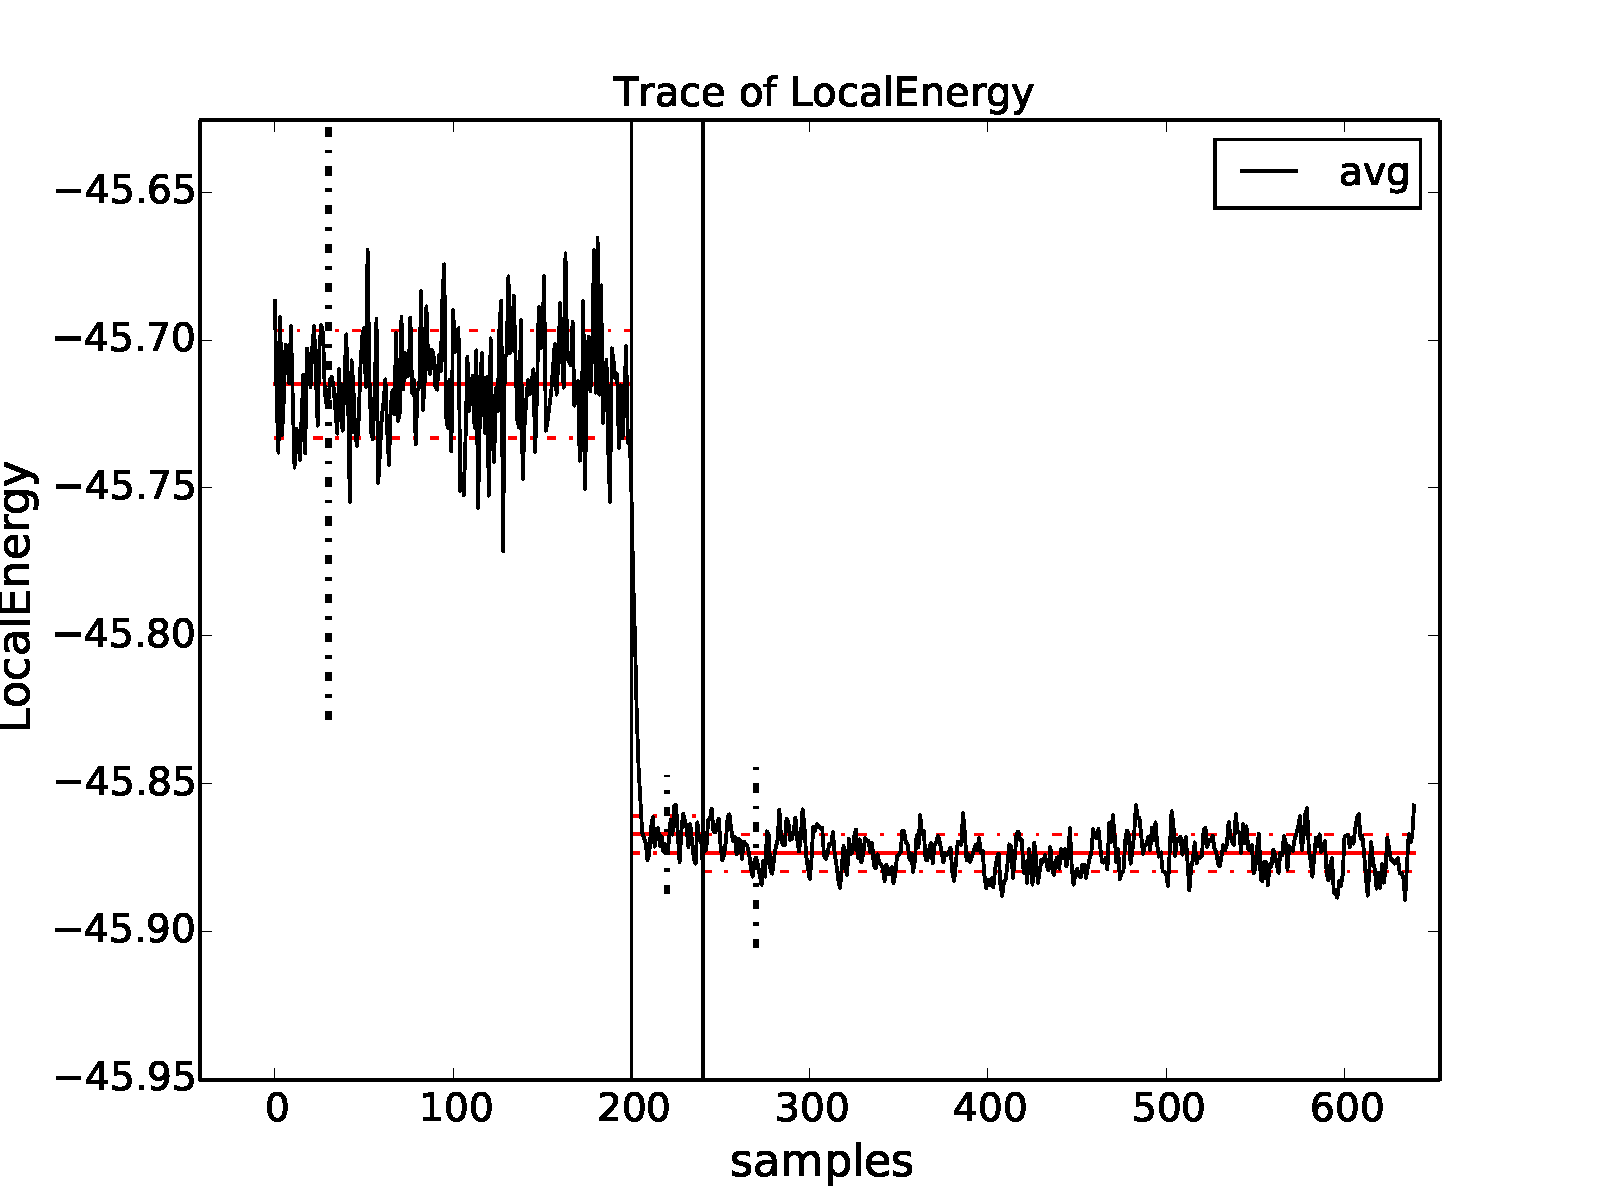
\includegraphics[trim = 0mm 0mm 0mm 0mm, clip,width=0.75\columnwidth]{./figures/qmca_twist_average_trace.png}
\else
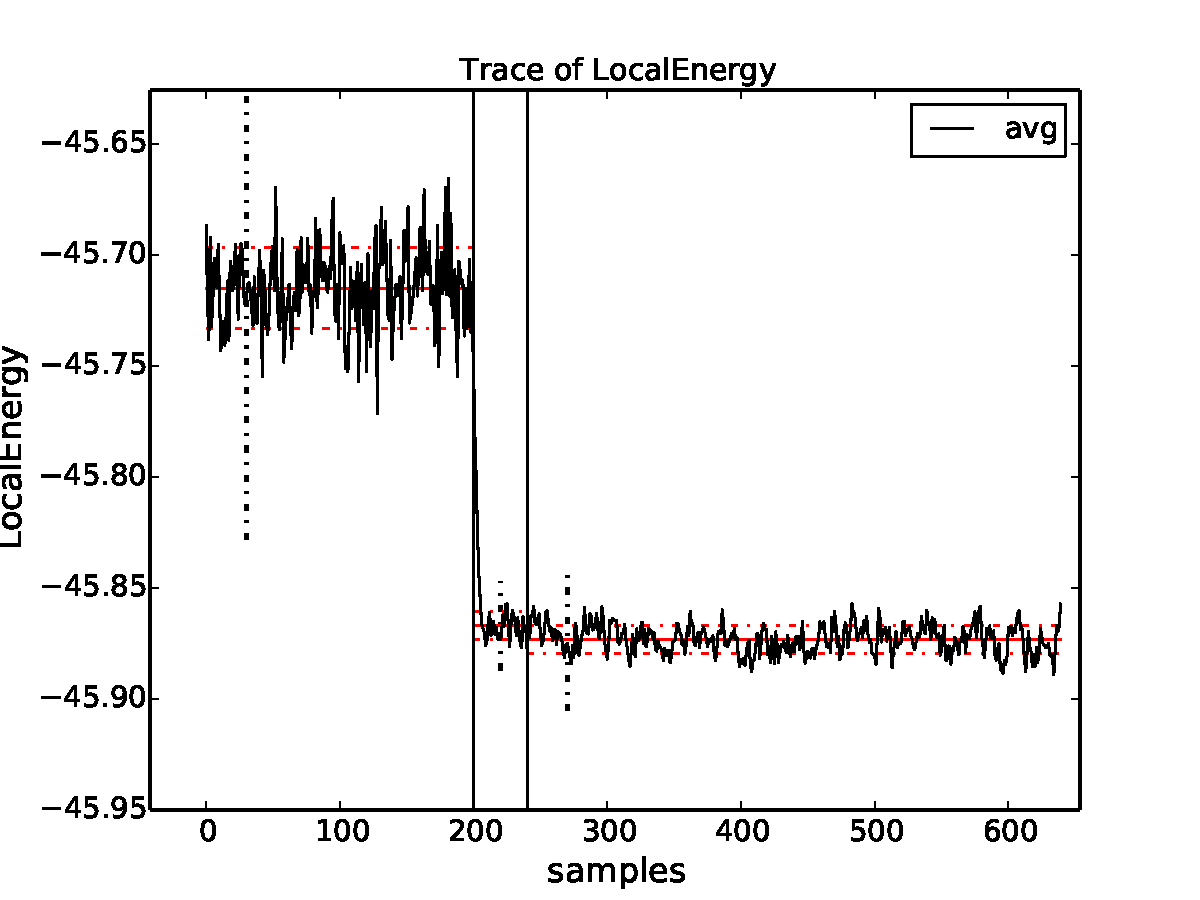
\includegraphics[trim = 0mm 0mm 0mm 0mm, clip,width=0.75\columnwidth]{./figures/qmca_twist_average_trace.pdf}
\fi
\end{center}
\caption{Twist averaged energy trace from VMC to DMC for an 8 supercell of diamond obtained with \texttt{qmca}.}
\label{fig:qmca_twist_average}
\end{figure}

As can be seen from the Fig. \ref{fig:qmca_twist_overlap}, some of the twist 
angles are degenerate. This is seen more clearly in the text output:
\begin{shade}
>qmca -q ev -e 30 *s002.scalar*
                            LocalEnergy               Variance           ratio 
qmc.g000  series 2  -45.264510 +/- 0.001942   1.057065 +/- 0.002318   0.0234 
qmc.g001  series 2  -46.035511 +/- 0.001806   1.015992 +/- 0.002836   0.0221 
qmc.g002  series 2  -46.035410 +/- 0.001538   1.015039 +/- 0.002661   0.0220 
qmc.g003  series 2  -46.047285 +/- 0.001898   1.018219 +/- 0.002588   0.0221 
qmc.g004  series 2  -46.034225 +/- 0.002539   1.013420 +/- 0.002835   0.0220 
qmc.g005  series 2  -46.046731 +/- 0.002963   1.018337 +/- 0.004109   0.0221 
qmc.g006  series 2  -46.047133 +/- 0.001958   1.021483 +/- 0.003082   0.0222 
qmc.g007  series 2  -45.476146 +/- 0.002065   1.070456 +/- 0.003133   0.0235 
\end{shade}
\noindent
The degenerate twists grouped by set are $\{0\}$, $\{1,2,4\}$, $\{3,5,6\}$, 
$\{7\}$.

Alternatively, the run could have been performed at \emph{only} the four 
unique (irreducible) twist angles.  We will emulate this situation by 
analyzing data for twists 0, 1, 3, and 7 only.  In a production setting 
with irreducibly weighted twists, run would be performed on these twists 
alone; we reuse the uniform twist data for illustration purposes only.  

We can use \texttt{qmca} to perform twist averaging with different 
weights applied to each twist
\begin{shade}
>qmca -a -w '1 3 3 1' -q ev -e 30 *g000*2*sc* *g001*2*sc* *g003*2*sc* *g007*2*sc*
                            LocalEnergy               Variance           ratio 
avg  series 2  -45.873631 +/- 0.001044   1.028769 +/- 0.001520   0.0224 
\end{shade}
\noindent
yielding a total energy value of $-45.874(1)$ Ha, in agreement with the 
uniform weighted twist average performed above.  

The decision of whether or not to perform irreducible weighted twist 
averaging should be made on the basis of efficiency.  The relative 
efficiency of irreducible vs. uniform weighted twist averaging 
depends on the irreducible weights and the ratio of the lengths of 
the available sampling and equilibration periods.  A formula for 
the relative efficiency of these two cases is derived and discussed 
in more detail in Appendix \ref{sec:app_ta_efficiency}.


\subsection{Setting output units}
\label{sec:qmca_output_units}
Estimates outputted by \texttt{qmca} are in Hartree units by 
default.  The output units for energetic quantities can be 
changed by using the ``\texttt{-u}'' option.  

\vspace{3mm}
\noindent
Energy in Hartrees:
\begin{shade}
>qmca -q e -u Ha -e 20 qmc.s002.scalar.dat
qmc  series 2  LocalEnergy           =  -46.032960 +/- 0.002077
\end{shade}

\noindent
Energy in electron volts:
\begin{shade}
>qmca -q e -u eV -e 20 qmc.s002.scalar.dat
qmc  series 2  LocalEnergy           =  -1252.620565 +/- 0.056521 
\end{shade}

\noindent
Energy in Rydbergs:
\begin{shade}
>qmca -q e -u rydberg -e 20 qmc.s002.scalar.dat
qmc  series 2  LocalEnergy           =  -92.065919 +/- 0.004154   
\end{shade}

\noindent
Energy in kilojoules per mole:
\begin{shade}
>qmca -q e -u kj_mol -e 20 qmc.s002.scalar.dat
qmc  series 2  LocalEnergy           =  -120859.512998 +/- 5.453431   
\end{shade}


\subsection{Speeding up trace plotting}
\label{sec:qmca_fast_trace_plot}
When working with many files or files with many entries, 
\texttt{qmca} may take a long time to produce plots.  The time 
delay is actually due to the autocorrelation time estimate 
used to calculate error bars.  The calculation time for 
the autocorrelation scales as $\mathcal{O}(M^2)$, with $M$ being 
the number of statistical samples.  If you are only interested 
in plotting traces and not in the estimated error bars, the 
autocorrelation time estimation can be turned off with the 
``\texttt{--noac}'' option:
\begin{shade}
>qmca -t -q e -e 20 --noac qmc.s002.scalar.dat
\end{shade}
\noindent
Please note that the resulting error bars printed to the console 
will be underestimated and are not meaningful.  Do \emph{not} 
use ``\texttt{--noac}'' in conjunction with the ``\texttt{-p}'' 
plotting option as these plots are of no use without meaningful 
error bars.


\subsection{Short usage examples}
\label{sec:qmca_short_examples}
\noindent
Plotting a trace of the local energy:
\begin{shade}
>qmca -t -q e *scalar*
\end{shade}
\noindent
Applying an equilibration cutoff to VMC data (series 0):
\begin{shade}
>qmca -q e -e 30 *s000.scalar*
\end{shade}
\noindent
Applying the same equilibration cutoff to VMC and DMC data (series 0, 1, 2):
\begin{shade}
>qmca -q e -e 20 *scalar*
\end{shade}
\noindent
Applying different equilibration cutoffs to VMC and DMC data (series 0, 1, 2):
\begin{shade}
>qmca -q e -e '30 20 40' *scalar*
\end{shade}
\noindent
Obtaining the energy, variance, and variance/energy ratio for all series:
\begin{shade}
>qmca -q ev -e 30 *scalar*
\end{shade}
\noindent
Overlaying plots of mean + error bar for energy and variance for separate 
two- and three- body Jastrow optimization runs:
\begin{shade}
>qmca -po -q ev ./optJ2/*scalar* ./optJ3/*scalar*
\end{shade}
\noindent
Obtaining the acceptance ratio:
\begin{shade}
>qmca -q ar -e 30 *scalar*
\end{shade}
\noindent
Obtaining the average DMC walker population:
\begin{shade}
>qmca -q nw -e 400 *s002.dmc.dat
\end{shade}
\noindent
Obtaining the Monte Carlo efficiency:
\begin{shade}
>qmca -q eff -e 30 *scalar*
\end{shade}
\noindent
Obtaining the total wallclock time per series:
\begin{shade}
>qmca -q tt -e 0 *scalar*
\end{shade}
\noindent
Obtaining the average wallclock time spent per block:
\begin{shade}
>qmca -q bc -e 0 *scalar*
\end{shade}
\noindent
Obtaining a subset of desired quantities:
\begin{shade}
>qmca -q 'e v ar eff' -e 30 *scalar*
\end{shade}
\noindent
Obtaining all available quantities:
\begin{shade}
>qmca -e 30 *scalar*
\end{shade}
\noindent
Obtaining the twist averaged total energy with uniform weights:
\begin{shade}
>qmca -a -q e -e 40 *g*s002.scalar.dat
\end{shade}
\noindent
Obtaining the twist averaged total energy with specific weights:
\begin{shade}
>qmca -a -w '1 3 3 1' -q e -e 40 *g*s002.scalar.dat
\end{shade}
\noindent
Obtaining the local, kinetic, and potential energies in eV:
\begin{shade}
>qmca -q ekp -e 30 -u eV *scalar*
\end{shade}



\subsection{Production quality checklist}
\label{sec:qmca_production_checklist}

\begin{enumerate}
  \item{Inspect the trace plots (``\texttt{-t}'' option) for any 
    oddities in the data.  Typical behavior is a short equilibration 
    period followed by benign fluctuations around a clear mean value.  
    There should not be any large spikes in the data. This applies 
    to \emph{all} runs (VMC, optimization, DMC, etc.).}

  \item{Remove all equilibration steps (``\texttt{-e}'' option) from 
    the data by inspecting the trace plot.}

  \item{Check the quality of the orbitals (standalone Jastrow-less 
    VMC or sometimes the first \texttt{scalar} file produced during 
    optimization) by inspecting the variance/energy ratio 
    ``\texttt{qmca -q ev *scalar*}''.  For pseudopotential systems 
    without a Jastrow, the variance/energy ratio should not exceed 
    $0.2$ Ha, otherwise there is a problem with the orbitals.}

  \item{Check the quality of the optimized Jastrow factor by inspecting 
    the variance/energy ratio.  For pseudopotential systems with a 
    Jastrow, the variance/energy ratio should not exceed $0.04$ Ha 
    for pseudopotential systems.  A good Jastrow is indicated by a 
    variance/energy ratio in the range $0.01-0.03$ Ha.  A value less 
    than $0.01$ Ha is difficult to achieve.}

  \item{Confirm that the optimization has converged by plotting the 
    energy and variance vs. optimization series 
    (``\texttt{qmca -p -q ev *scalar*}'').  Do not assume that 
    optimization has converged in only a few cycles.  Use at least 
    10 cycles of with around 100,000 samples unless you already have 
    experience with the system in question.}

  \item{Optimize Jastrow factors according to energy minimization to 
    reduce locality errors arising from the use of non-local 
    pseudopotentials in DMC.  A good approach is to optimize with a 
    few cycles of variance minimization followed by several cycles of 
    energy minimization.}

  \item{Occasionally try optimizing with more samples and/or cycles 
    to see if improved results are obtained.}

  \item{If using a B-spline representation of the orbitals, converge 
    the VMC energy and variance with respect to the mesh size (controlled 
    via meshfactor).  This is best done in the presence of any 
    Jastrow factor to reduce noise.  Consider using the hybrid LMTO 
    representation of the orbitals as this can reduce both the VMC/DMC 
    variance and DMC timestep error in addition to saving memory.}

  \item{Check the variance/energy ratio of all production VMC and DMC 
    calculations.  In all cases the DMC ratio should be slightly 
    less than the VMC one and both should abide the guidelines above, 
    \emph{i.e.} the ratio should be less than $0.04$ Ha for 
    pseudopotential systems.  The production ratio should also be 
    consistent with what is observed during wavefunction optimization.}

  \item{Be aware of population control bias in DMC.  Run with a 
    population of $\sim 2000$ or greater.  Occasionally repeat a run 
    using a larger population to explicitly confirm that population 
    control bias is small.}

  \item{Check the stability of the DMC walker population by plotting 
    the trace of the population size (``\texttt{qmca -t -q nw *dmc.dat}'').  
    Verify that the average walker population is consistent with 
    the requested value provided in the input.}

  \item{In DMC, perform a timestep study to either 1) obtain 
    extrapolated results, or 2) obtain a timestep for future 
    production where an energy difference shows convergence 
    (\emph{e.g.} a band gap or defect formation energy).  For 
    pseudopotential systems, converged timesteps for many systems 
    are in the range $0.002-0.01$ Ha$^{-1}$, but the actual converged 
    timestep must be explicitly checked.}

  \item{In periodic systems, converge the total energy with respect to 
    the size of the twist/k-point grid.  Results for smaller systems 
    can easily be transferred to larger ones (\emph{e.g.} a 2x2x2 twist 
    grid in a 2x2x2 tiled cell is equivalent to a 1x1x1 twist grid in a 
    4x4x4 tiled cell)}.

  \item{In periodic systems, perform finite size extrapolation 
    including two body corrections (needed for cohesive energy/phase 
    stability studies) unless it can be shown that finite size effects 
    cancel for the energy difference in question (\emph{e.g.} some 
    defect formation energies).}

\end{enumerate}


\section{Using the qfit tool for statistical timestep extrapolation and curve fitting}
\label{sec:qfit}

The \texttt{qfit} tool is used to provide statistical estimates of
curve fitting parameters based on QMCPACK data.  While \texttt{qfit}
will eventually support many types of fitted curves (\emph{e.g.} Morse
potential binding curves, various equation of state fitting curves, etc.),
it is currently limited to estimating fitting parameters related to
timestep extrapolation.

\subsection{The jack-knife statistical technique}
The \texttt{qfit} tool obtains estimates of fitting parameter
means and associated error bars via the ``jack-knife''
technique.  The jack-knife method is a powerful and general tool
to obtain meaningful error bars for any quantity that is related
in a non-linear fashion to an underlying set of statistical data.
For this reason, we give a brief overview of the jack-knife
technique before proceeding with usage instructions for the
\texttt{qfit} tool.

Consider $N$ statistical variables $\{x_n\}_{n=1}^N$ that have
been outputted by one or more simulation runs.  If we have
$M$ samples of each of the $N$ variables, then the mean values
of each these variables can be estimated in the standard way,
i.e. $\bar{x}_n\approx \tfrac{1}{M}\sum_{m=1}^Mx_{nm}$.

Suppose we are interested in $P$ statistical quantities
$\{y_p\}_{p=1}^P$ that are related to the original $N$ variables
by a known multidimensional function $F$:
\begin{align}
  y_1,y_2,\ldots,y_P &= F(x_1,x_2,\ldots,x_N)\quad \textrm{or} \nonumber \\
  \vec{y} &= F(\vec{x})
\end{align}
The relationship implied by $F$ is completely general. 
For example the $\{x_n\}$ might be elements of a matrix
with $\{y_p\}$ being the eigenvalues, or $F$ might be
a fitting procedure for $N$ energies at different timesteps
with $P$ fitting parameters.  An approximate guess at the mean
value of $\vec{y}$ can be obtained by evaluating $F$ at the mean
value of $\vec{x}$ (i.e. $F(\bar{x}_1\ldots\bar{x}_N)$), but with
this approach we have no way to estimate the statistical error 
bar of any $\bar{y}_p$.

In the jack-knife procedure, the statistical variability intrinsic
to the underlying data $\{x_n\}$ is used to obtain estimates of the
mean and error bar of $\{y_p\}$.  We first construct a new set of $x$
statistical data by taking the average over all samples but one:
\begin{align}
  \tilde{x}_{nm} = \frac{1}{N-1}(N\bar{x}_n-x_{nm})\qquad m\in [1,M]
\end{align}
The result is a distribution of approximate $x$ mean values.  These
are used to construct a distribution of approximate means for $y$:
\begin{align}
  \tilde{y}_{1m},\ldots,\tilde{y}_{Pm} = F(\tilde{x}_{1m},\ldots,\tilde{x}_{Nm}) \qquad m\in [1,M]
\end{align}
Estimates for the mean and error bar of the quantities of
interest can finally be obtained using the formulas below:
\begin{align}
  \bar{y}_p &= \frac{1}{M}\sum_{m=1}^M\tilde{y}_{pm} \\
  \sigma_{y_p} &= \sqrt{\frac{M-1}{M}\left(\sum_{m=1}^M\tilde{y}_{pm}^2-M\bar{y}_p^2\right)}
\end{align}


\subsection{Performing timestep extrapolation}
In this section, we use a 32 atom supercell of MnO as an example
system for timestep extrapolation.  Data for this system has been
collected in DMC using the following sequence of timesteps:
$0.04,~0.02,~0.01,~0.005,~0.0025,~0.00125$ Ha$^{-1}$.  For a typical
production pseudopotential study, timesteps in the range
$0.02-0.002$ Ha$^{-1}$ are usually sufficient and it is recommended
to increase the number of steps/blocks by a factor of two when
the timestep is halved.  In order to perform accurate statistical
fitting, we must first understand the equilibration and autocorrelation
properties of the inputted local energy data.  After plotting the
local energy traces (\texttt{qmca -t -q e -e 0 ./qmc*/*scalar*})
it is clear that an equilibration period of $30$ blocks is reasonable.
Approximate autocorrelation lengths are also obtained with \texttt{qmca}:
\begin{shade}
>qmca -e 30 -q e --sac ./qmc*/qmc.g000.s002.scalar.dat
./qmc_tm_0.00125/qmc.g000 series 2 LocalEnergy = -3848.234513 +/- 0.055754  1.7 
./qmc_tm_0.00250/qmc.g000 series 2 LocalEnergy = -3848.237614 +/- 0.055432  2.2 
./qmc_tm_0.00500/qmc.g000 series 2 LocalEnergy = -3848.349741 +/- 0.069729  2.8 
./qmc_tm_0.01000/qmc.g000 series 2 LocalEnergy = -3848.274596 +/- 0.126407  3.9 
./qmc_tm_0.02000/qmc.g000 series 2 LocalEnergy = -3848.539017 +/- 0.075740  2.4 
./qmc_tm_0.04000/qmc.g000 series 2 LocalEnergy = -3848.976424 +/- 0.075305  1.8 
\end{shade}
\noindent
The autocorrelation must be removed from the data prior to jack-knifing
and so we will reblock the data by a factor of 4.

The \texttt{qfit} tool can be used in the following way to obtain
a linear timestep fit of the data:
\begin{shade}
>qfit ts -e 30 -b 4 -s 2 -t '0.00125 0.0025 0.005 0.01 0.02 0.04' ./qmc*/*scalar*
fit function  : linear
fitted formula: (-3848.193 +/- 0.037) + (-18.95 +/- 1.95)*t
intercept     : -3848.193 +/- 0.037  Ha
\end{shade}
The input arguments are as follows: \texttt{ts} indicates we are
performing a timestep fit, ``\texttt{-e 30}'' is the equilibration period
removed from each set of scalar data, ``\texttt{-b 4}'' indicates the data
will be reblocked by a factor of 4 (\emph{e.g.} a file containing 400 \
entries will be block averaged into a new set of 100 prior to jack-knife
fitting), ``\texttt{-s 2}'' indicates that the timestep data begins with
series 2 (scalar files matching \texttt{*s000*} or \texttt{*s001*} are
to be excluded), and ``\texttt{-t } '0.00125 0.0025 0.005 0.01 0.02 0.04' ''
provides a list of timestep values corresponding to the inputted scalar
files.  The ``\texttt{-e}'' and ``\texttt{-b}'' options can receive a
list of file-specific values (same format as ``\texttt{-t}'') if desired.
As can be seen from the text output, the parameters for the linear fit
are printed with error bars obtained with jack-knife resampling and
the zero timestep ``intercept'' is $-3848.19(4)$ Ha.  In addition to
text output, the command above will result in a plot of the fit with
the zero timestep value shown as a red dot, as shown in the left
panel of Fig.~\ref{fig:qfit_timestep}.

\begin{figure}
  \centering
  \parbox{0.47\linewidth}{%
    \ifdefined\HCode%
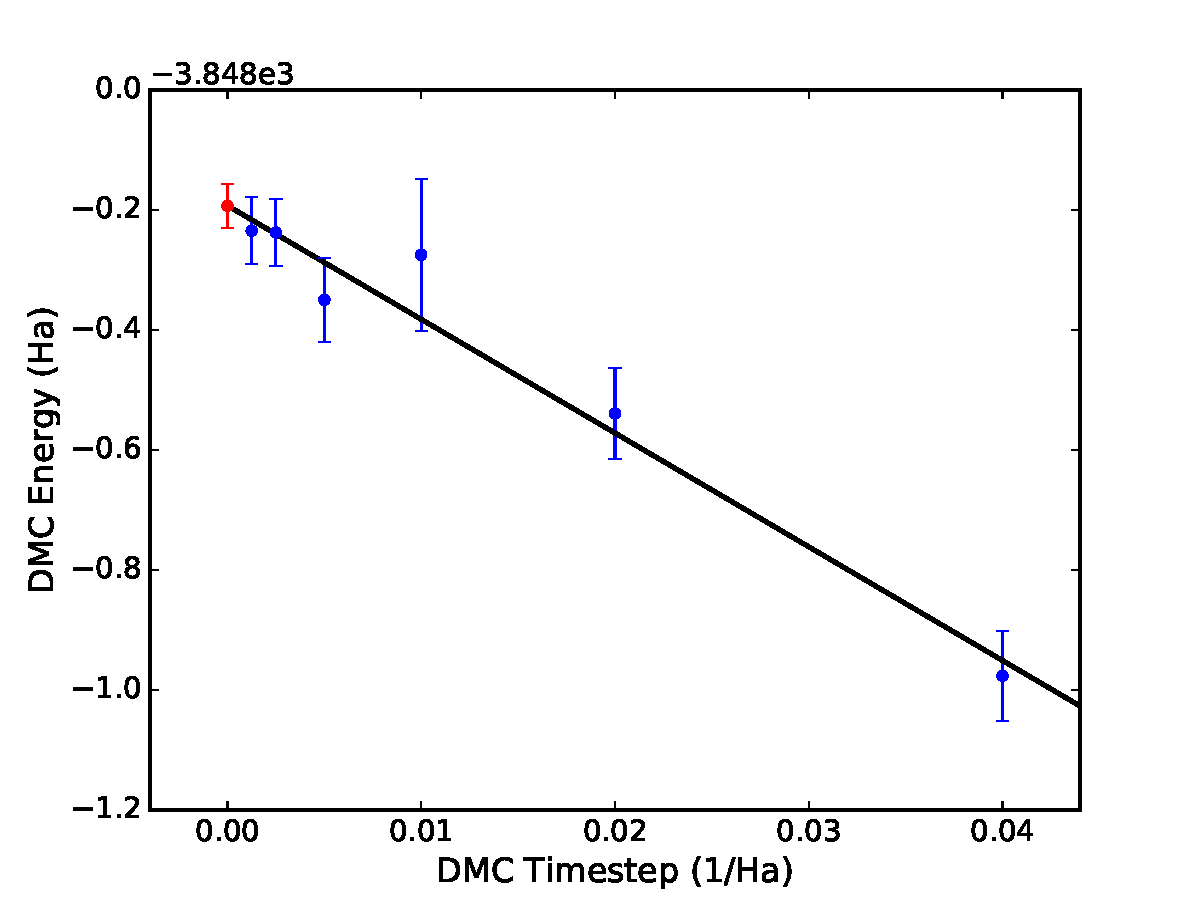
\includegraphics[trim=0mm 0mm 4mm 0mm,clip,width=\linewidth]{./figures/qfit_timestep_linear.png}%
\else%
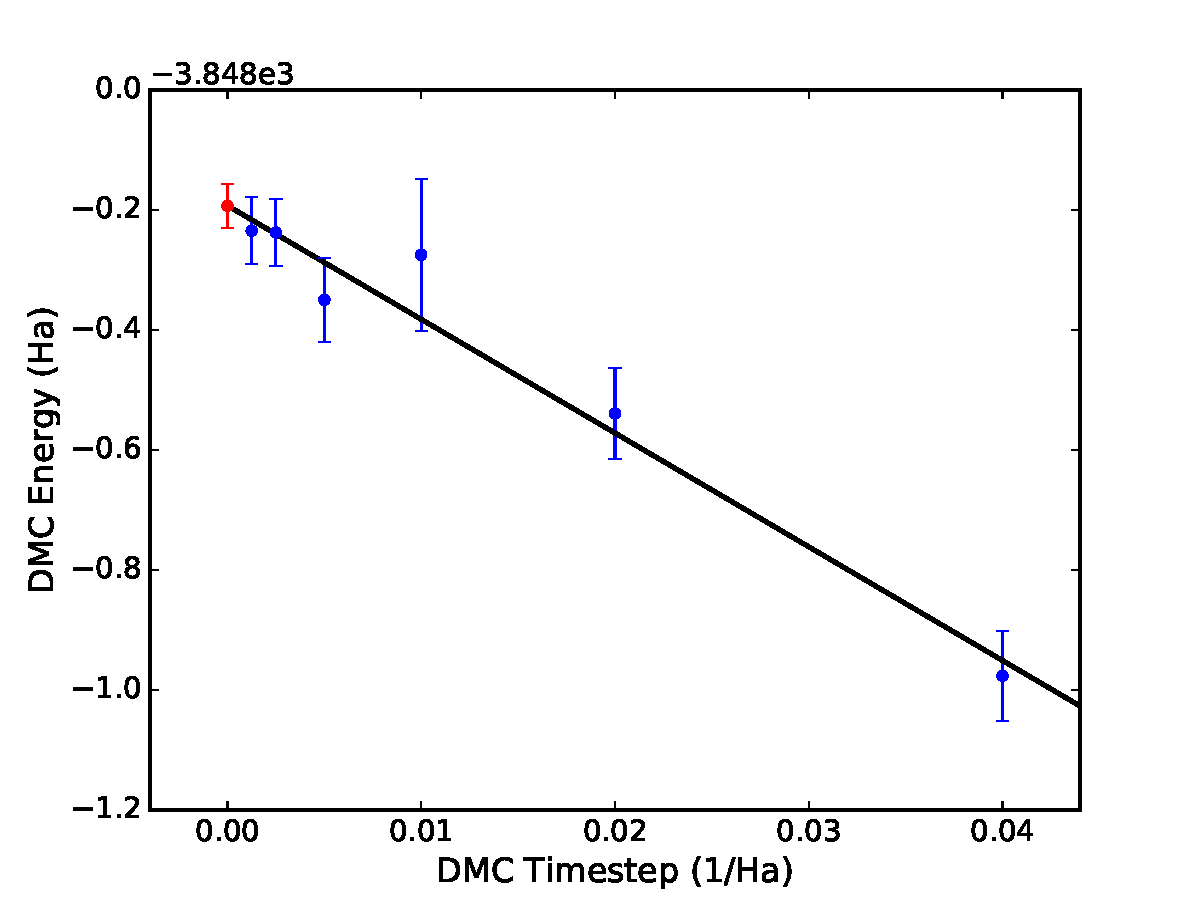
\includegraphics[trim=0mm 0mm 4mm 0mm,clip,width=\linewidth]{./figures/qfit_timestep_linear.pdf}%
\fi%
  }%
  \qquad%
  \begin{minipage}{0.47\linewidth}%
    \ifdefined\HCode%
    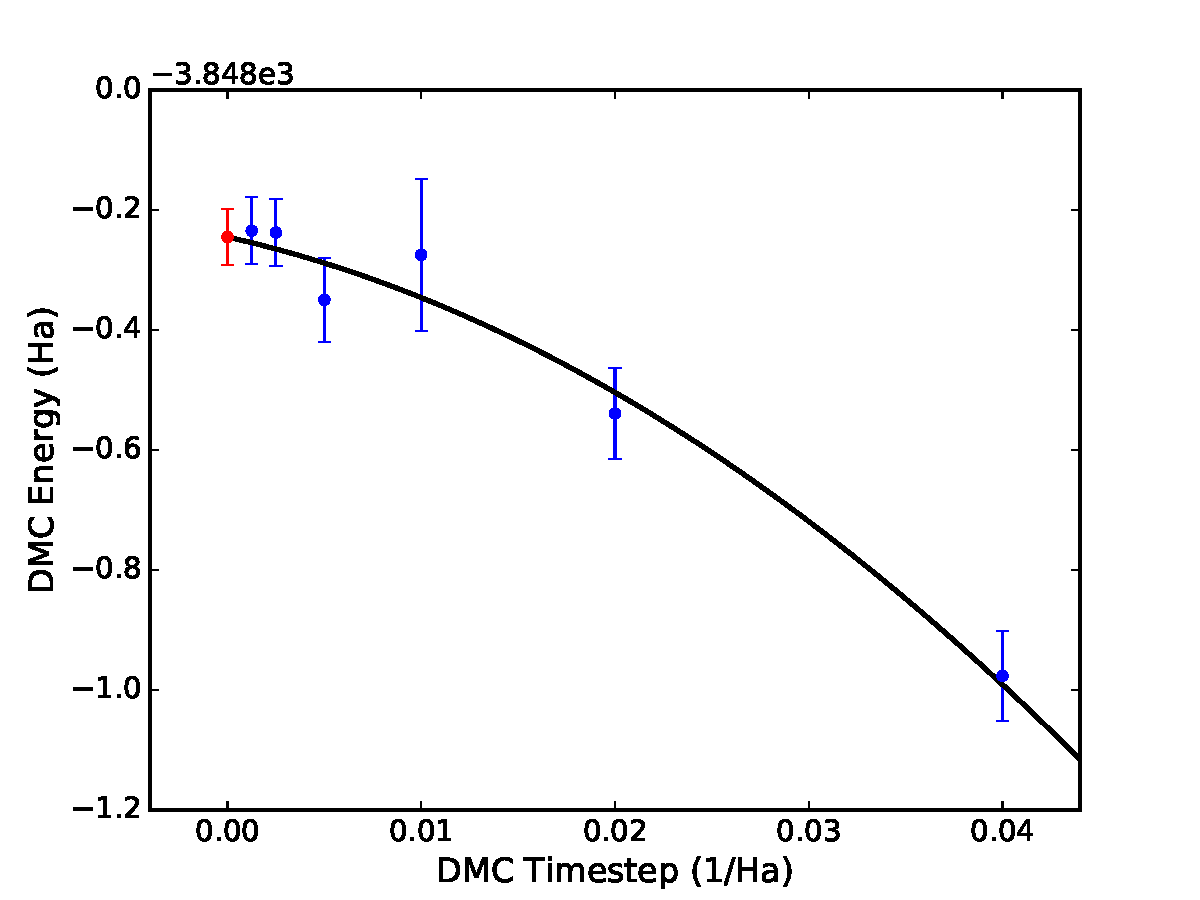
\includegraphics[trim=2mm 0mm 4mm 0mm,clip,width=\linewidth]{./figures/qfit_timestep_quadratic.png}%
\else%
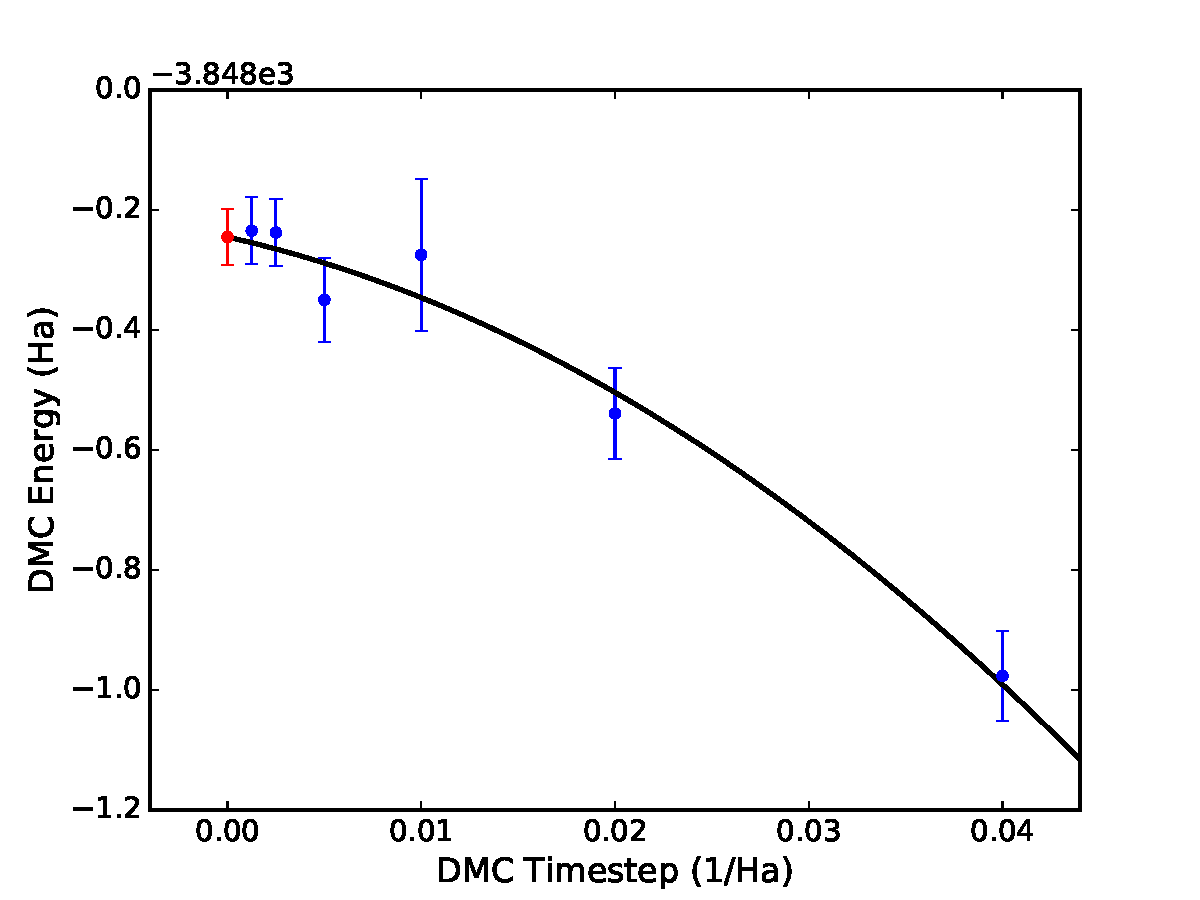
\includegraphics[trim=2mm 0mm 4mm 0mm,clip,width=\linewidth]{./figures/qfit_timestep_quadratic.pdf}%
\fi%
  \end{minipage}%
  \caption{Linear (left) and quadratic (right) timestep fits to DMC data for a 32 atom supercell of MnO obtained with \texttt{qfit}.  Zero timestep estimates are indicated by the red data point on the left side of either panel.}
  \label{fig:qfit_timestep}
\end{figure}

Different fitting functions are supported via the ``\texttt{-f}'' option.
Currently supported options include \texttt{linear} ($a+bt$),
\texttt{quadratic} ($a+bt+ct^2$), and \texttt{sqrt} ($a+b\sqrt{t}+ct$).
Results for a quadratic fit are shown below as well as in the right
panel of Fig.~\ref{fig:qfit_timestep}.
\begin{shade}
>qfit ts -f quadratic -e30 -b4 -s2 -t '0.00125 0.0025 0.005 0.01 0.02 0.04' ./qmc*/*scalar*
fit function  : quadratic
fitted formula: (-3848.245 +/- 0.047) + (-7.25 +/- 8.33)*t + (-285.00 +/- 202.39)*t^2
intercept     : -3848.245 +/- 0.047  Ha
\end{shade}
In this case we find a zero timestep estimate of $-3848.25(5)$ Ha$^{-1}$.
A timestep of $0.04$ Ha$^{-1}$ might be on the large side to include in
timestep extrapolation and it is likely to have an outsize influence
in the case of linear extrapolation.  Upon excluding this point, linear
extrapolation yields a zero timestep value of $-3848.22(4)$ Ha$^{-1}$.
It should be noted that quadratic extrapolation can result in intrinsically
larger uncertainty in the extrapolated value.  For example, when the $0.04$
Ha$^{-1}$ point is excluded the uncertainty grows by 50\% and we obtain an
estimated value of $-3848.28(7)$ instead.



\section{Densities and spin-densities}
\label{sec:densities}

\section{Energy densities}
\label{sec:energydensities}






\section{Auxiliary-Field Quantum Monte Carlo}
\label{sec:afqmc}
Unlike diffusion Monte Carlo that works in first quantized representation and in configuration space, the auxiliary-field QMC (AFQMC) methods work in second quantized representation and in an auxiliary-field space to represent the wave function or density matrix and to carry out the integrations in evaluating ground-state properties. The idea of AFQMC is to constrain the phase of the overlap of the sampled Slater determinants with a trial wave function. It eliminates the phase instability and restores low-power ($N^3$) computational scaling. AFQMC applies Trotter approximation and Hubbard-Stratonovich (HS) transformation to obtain the propagator, which converts an interacting system into non-interacting systems in fluctuating external auxiliary-fields. The sum over all configurations of auxiliary fields recovers the interaction.

The input file has six basic xml-blocks: \texttt{AFQMCInfo}, \texttt{Hamiltonian}, \texttt{Wavefunction}, \texttt{WalkerSet}, \texttt{Propagator}, and \texttt{execute}.  The first five define input structures required for various types of calculations. The \texttt{execute} block represents actual calculations and takes as input the other blocks. 
Non-execution blocks are parsed first, followed by a second pass where execution blocks are parsed (and executed) in order. All blocks contain a ``name'' argument, which is used to identify the resulting block. For example, in the previous example, multiple Hamiltonian objects with different names can be defined. The one actually used in the calculation is the one passed to ``execute'' as ham.
\begin{lstlisting}[caption=The following is an example input file in AFQMC.]
<?xml version="1.0"?>
<simulation method="afqmc">
  <project id="Carbon" series="0"/>

  <AFQMCInfo name="info0">
    <parameter name="NMO">32</parameter>
    <parameter name="NAEA">16</parameter>
    <parameter name="NAEB">16</parameter>
  </AFQMCInfo>

  <Hamiltonian name="ham0" type="SparseGeneral" info="info0">
    <parameter name="filetype">hdf5</parameter>
    <parameter name="filename">../fcidump.h5</parameter>
  </Hamiltonian>

  <Wavefunction name="wfn0" info="info0">
    <ImpSamp name="impsamp0" type="PureSD" init="ground" >
      <parameter name="filetype">none</parameter>
    </ImpSamp>
  </Wavefunction>

  <WalkerSet name="wset0" type="distributed">
  </WalkerSet>

  <Propagator name="prop0" info="info0">
  </Propagator>

  <execute wset="wset0" ham="ham0" wfn="wfn0" prop="prop0" info="info0">
    <parameter name="timestep">0.005</parameter>
    <parameter name="blocks">10000</parameter>
    <parameter name="nWalkers">20</parameter>
  </execute>

</simulation>
\end{lstlisting}

%The following table lists some of the most practical parameters in the \texttt{execute} block
%The following table lists some of the practical parameters
\begin{table}[h]
\begin{center}
\begin{tabularx}{\textwidth}{l l l l l l }
\hline
\multicolumn{6}{l}{\texttt{afqmc} method} \\
\hline
\multicolumn{6}{l}{parameters in \texttt{AFQMCInfo}} \\
   &   \bfseries name     & \bfseries datatype & \bfseries values & \bfseries default   & \bfseries description \\
%   &   \texttt{name            } &  argument    &         & no & unique name that identifies the xml-block \\
   &   \texttt{NMO             } &  integer     & $\ge 0$ & no & number of molecular orbitals \\
   &   \texttt{NAEA            } &  integer     & $\ge 0$ & no & number of active electrons of spin up \\
   &   \texttt{NAEB            } &  integer     & $\ge 0$ & no & number of active electrons of spin down \\
%   &   \texttt{NCA            } &  integer     & $\ge 0$ & 0 & number of core electrons of spin up \\
%   &   \texttt{NCB            } &  integer     & $\ge 0$ & 0 & number of core electrons of spin down \\
\multicolumn{6}{l}{parameters in \texttt{Hamiltonian}}  \\
%   &   \bfseries name     & \bfseries datatype & \bfseries values & \bfseries default   & \bfseries description \\
%   &   \texttt{name            } &  argument   &               & no   & unique name that identifies the xml-block \\
   &   \texttt{type            } &  argument   & SparseGeneral & no   & type of \texttt{Hamiltonian} \\
   &   \texttt{info            } &  argument   &               &      & name of \texttt{AFQMCInfo} block \\\\
   &   \texttt{filename        } &  string     &               & no   & name of file with the hamiltonian \\
   &   \texttt{filetype        } &  string     & fcidump       & no   & ascii based format of molpro, VASP, pyscf, etc. \\
   &   \texttt{                } &             & hdf5          &      & native hdf5-based format of QMCPACK  \\
%   &   \texttt{cutoff\_1bar            } &  real     &  & 1e-8 & cutoff applied to integrals during reading \\
%   &   \texttt{cutoff\_decomposition   } &  real     &  & 1e-6 & cutoff used to stop the iterative cycle in the generation of the Cholesky decomposition of the 2-electron integrals \\
\multicolumn{6}{l}{parameters in \texttt{Wavefunction}}\\
%   &   \bfseries name     & \bfseries datatype & \bfseries values & \bfseries default   & \bfseries description \\
%   &   \texttt{name            } &  argument   &             & no   & unique name that identifies the xml-block \\
   &   \texttt{info            } &  argument   &             &      & name of \texttt{AFQMCInfo} block \\
   &   \texttt{ImpSamp         } &  xml-block  &             & no   & defines the trial wave-function \\
%   &   \texttt{name            } &  argument   &             & no   & unique name that identifies the xml-block \\
   &   \texttt{type            } &  argument   & PureSD      & no   & single slater determinant trial wave-function \\
   &   \texttt{                } &             & MultiPureSD &      & linear combination of Slater Determinants \\
   &   \texttt{                } &             & GenSD       &      & single determinant w/o rotated 2-e integrals \\
   &   \texttt{filetype        } &  string     & ascii       & no   & ascii data file type \\
   &   \texttt{                } &             & hdf5        &      & hdf5 data file type \\
   &   \texttt{                } &             & none        &      & no input file needed, requires init=``ground'' \\
\multicolumn{6}{l}{parameters in \texttt{WalkerSet}} \\
 %  &   \bfseries name     & \bfseries datatype & \bfseries values & \bfseries default   & \bfseries description \\
%   &   \texttt{name            } &  argument   &             & no   & unique name that identifies the xml-block \\
   &   \texttt{type            } &  argument   & distributed & no   & type of walker container: standard \\
   &   \texttt{                } &             & local       &      & simple but inefficient version. \\
\multicolumn{6}{l}{parameters in \texttt{Propagator}} \\
%   &   \bfseries name     & \bfseries datatype & \bfseries values & \bfseries default   & \bfseries description \\
%   &   \texttt{name            } &  argument   &       & no    & unique name that identifies the xml-block \\
   &   \texttt{type            } &  argument   & afqmc & afqmc & type of propgator \\
   &   \texttt{                } &             &  vmc  &       & not yet functioning \\
   &   \texttt{info            } &  argument   &       &       & name of \texttt{AFQMCInfo} block \\
\multicolumn{6}{l}{parameters in \texttt{execute}} \\
%   &   \bfseries name     & \bfseries datatype & \bfseries values & \bfseries default   & \bfseries description \\
%   &   \texttt{name            } &  argument    &         & no   & unique name that identifies the xml-block \\
   &   \texttt{wset            } &  argument    &         &      &  \\
   &   \texttt{ham             } & argument     &         &      &  \\
   &   \texttt{wfn             } & argument     &         &      &  \\
   &   \texttt{prop            } & argument     &         &      &  \\
   &   \texttt{info            } &  argument    &         &      & name of \texttt{AFQMCInfo} block \\
   &   \texttt{nWalkers        } &  integer     & $\ge 0$ & 5    & initial number of walkers per task group   \\
   &   \texttt{timestep        } &  real        & $> 0$   & 0.01 & time step in 1/a.u. \\
   &   \texttt{blocks          } &  integer     & $\ge 0$ & 100  & number of blocks            \\
   &   \texttt{step            } &  integer     & $> 0$   & 1    & number of steps within a block \\
   &   \texttt{substep         } &  integer     & $> 0$   & 1    & number of substeps within a step \\
  \hline
\end{tabularx}
\end{center}
\end{table}

Additional information:\\

\texttt{AFQMCInfo}: input block that defines basic information about the calculation. It is passed to all other input blocks to propagate the basic information:
\texttt{<AFQMCInfo name="info0">}
\begin{itemize}
%\item \textbf{NMO}. Number of molecular orbitals, i.e., number of states in the single particle basis. 
%\item \textbf{NAEA}. Number of Active Electrons-Alpha, i.e., number of spin-up electrons.
%\item \textbf{NAEB}. Number of Active Electrons-Beta, i.e., number of spin-down electrons.
\item \textbf{NCA}. number of core electrons of spin up (only meaningful if reading ascii FCIDUMPs). Default: 0.
\item \textbf{NCB}. Number of core electrons of spin down (only meaningful if reading ascii FCIDUMPs). Default: 0.\\
\end{itemize}

\texttt{Hamiltonian}: controls the object that reads, stores and manages the hamiltonian. 
  \texttt{<Hamiltonian name="ham0" type="SparseGeneral" info="info0">}
\begin{itemize}
%\item \textbf{filename}. Name of file with the \texttt{Hamiltonian}. This is a required parameter.
%\item \textbf{filetype}. The type of file found in filename. Options are: fcidump, hdf5. fcidump is the ascii based format of molpro, VASP, pyscf, etc.; hdf5 is the native hdf5-based format  of QMCPACK and can also be generated by modified versions of pyscf and VASP. This is a required parameter.
\item \textbf{cutoff\_1bar}. Cutoff applied to integrals during reading. Any term in the hamiltonian smaller than this value is set to zero. (For filetype=``hdf5'', the cutoff is only applied to the 2-electron integrals). Default: 1e-8
\item \textbf{cutoff\_decomposition}. Cutoff used to stop the iterative cycle in the generation of the Cholesky decomposition of the 2-electron integrals. The generation of Cholesky vectors is stopped when the maximum error in the diagonal reaches this value. In case of an eigenvalue factorization, this becomes the cutoff applied to the eigenvalues. Only eigenvalues above this value are kept. Default: 1e-6
\item \textbf{hdf\_write\_file}. If a value is given, an hdf5 restart file for the \texttt{Hamiltonian} is generated. Default: ``'' (no file is generated)
\item \textbf{hdf\_write\_type}. What to store in the restart file. Options: ``integrals'': write directly the 1- and 2-electron integrals; ``factorized'': write the cholesky decomposition of the integrals; ``default'': Default value, write the type found in filetype.
\item \textbf{ascii\_write\_file} If a value is given, an ascii restart file for the \texttt{Hamiltonian} is generated. Default: ``'' (no file is generated)
\item \textbf{nblocks}. This parameter controls the distribution of the 2-electron integrals among processors. In the default behavior (nblocks=1), all nodes contain the entire list of integrals. If nblocks $>$ 1, the of nodes in the calculation will be split in nblocks groups. Each node in a given group contains the same subset of integrals and subsequently operates on this subset during  any further operation that requires the hamiltonian. The maximum number of groups is NMO. Currently only works for filetype=``hdf5'' and the file must contain integrals.  Not yet implemented for input hamiltonians in the form of Cholesky vectors or for ascii input. Coming soon!
    Default: No distribution
\item \textbf{printEig}. If ``yes'', prints additional information during the Cholesky decomposition.
    Default: no
\item \textbf{fix\_2eint}.  If this is set to ``yes'', orbital pairs that are found not to be positive definite are ignored in the generation of the Cholesky factorization. This is necessary if the 2-electron integrals are not positive definite due to round-off errors in their generation.
    Default: no \\
\end{itemize}

\texttt{Wavefunction}: controls the object that manages the trial wave-functions. This block expects a list of xml-blocks defining actual trial-wave functions for various roles. 
\texttt{<Wavefunction name="wfn0" info="info0">}
  \texttt{<ImpSamp name="impsamp0" type="PureSD">}
\begin{itemize}
\item \textbf{init}. Argument in ImpSamp. Selects pre-defined trial wave-functions if desired. 
Value: ground. Only for PureSD. Sets the trial wave-function to a block diagonal form. Diagonal in the occupied-occupied block and zero outside. This option corresponds to b
tate determinant (assuming orbitals ordered by increasing eigenvalue) in the orbital space that defines the hamiltonian. For a \texttt{Hamiltonian} generates based on HF orbitals, this generates a HF trial wave-function. (Only useful situation.)
\item \textbf{filename}. Name of file with wave-function information.
\item \textbf{cutoff}. cutoff applied to the terms in the calculation of the local energy. Only terms in the hamiltonian above this cutoff are included in the evaluation of the energy.
      Default: 1e-6
\item \textbf{nnodes}. Defines the parallelization of the local energy evaluation and the distribution of the \texttt{Hamiltonian} matrix (not to be confused with the list of 2-electron integrals managed by \texttt{Hamiltonian}. These are not the same.) If nnodes $>$ 1, the nodes in the simulation are split into groups of nnodes, each group works collectively in the evaluation of the local energy of their walkers. This helps distribute the effort involved in the evaluation of the local energy among the nodes in the group, but also distributes the memory associated with the wave-function among the nodes in the group.
      Default: No distribution
\item \textbf{hdf\_write\_file}. If provided, a restart file for the wave-function will be generated.
      Default: ``''
\item \textbf{runtype}. Unique to MultiPureSD with orthogonal expansions.
      Values: 0.  Use low memory algorithm. Much slower but has small memory requirements;
      1. Use high-memory algorithm. Faster but with significant memory requirements.
\item \textbf{fast}. Unique to MultiPureSD. If ``yes'', use fast-update algorithm with orthogonal expansions.
      Default: No
\item \textbf{Estimator}. Optional xml-block which defines a trial wave-function used for the calculation of energy averages.  It is used only during the collection of averages and doesn't influence the propagation. Note that this block must be set if an Estimator xml-block in the execute xml-block is specified. This must also be defined in order to calculate and print the energy in the case of hybrid propagation (see below). \\
\end{itemize}

\texttt{WalkerSet}: Controls the object that handles the set of walkers.
\texttt{<WalkerSet name="wset0" type="distributed">}
\begin{itemize}
\item \textbf{pop\_control}. Population control algorithm. Options: ``simple'': Uses a simple branching scheme with a fluctuating population. Walkers with weight above max\_weight are split into multiple walkers of weight reset\_weight. Walkers with weight below min\_weight are killed with probability (weight/min\_weight); ``pair'': Fixed-population branching algorithm, based on QWalk's branching algorithm. Pairs of walkers with weight above/below max\_weight/min\_weight are combined into 2 walkers with weights equal to $(w_1+w_2)/2$. The probability of replicating walker w1 (larger weight) occurs with probability $w_1/(w_1+w_2)$, otherwise walker w2 (lower weight) is replicated; ``comb'': Fixed-population branching algorithm based on the Comb method. Will be available in the next release. Default: ``pair''
\item \textbf{min\_weight}. Weight at which walkers are possibly killed (with probability weight/min\_weight). Default: 0.05
\item \textbf{max\_weight}. Weight at which walkers are replicated. Default: 4.0
\item \textbf{reset\_weight}. Weight to which replicated walkers are reset to. Default: 1.0
\item \textbf{extra\_spaces}. Number of empty spaces kept in the list. Useful to avoid constant reallocation. Default: 10 \\
\end{itemize}

\texttt{Propagator}: Controls the object that manages the propagators.
\texttt{<Propagator name="prop0" info="info0">}
\begin{itemize}
\item \textbf{cutoff}. Cutoff applied to Cholesky vectors. Elements of the Cholesky vectors below this value are set to zero.
    Default: 1e-6
\item \textbf{substractMF}. If ``yes'', apply mean-field substraction based on the ImpSamp trial wave-function. Must set to ``no'' to turn it off.
    Default: yes
\item \textbf{useCholesky}. If ``yes'', use iterative Cholesky decomposition to factorize 2-electron integral matrix. If ``no'', use eigenvalue decomposition (which is very slow and memory intensive).
    Default: yes
\item \textbf{vbias\_bound}. Upper bound applied to the vias potential. Components of the vias potential above this value are truncated there.
    Default: 3.0
\item \textbf{apply\_constrain}. If ``yes'', apply the phaseless constrain to the walker propagation. Currently, setting this to ``no'' produces unknown behavior, since free propagation algorithm has not been tested.
    Default: yes
\item \textbf{hybrid}. If ``yes'', use hybrid propagation algorithm. This propagation scheme doesn't use the local energy during propagation, leading to significant speed ups when its evaluation  cost is high. The local energy of the ImpSamp trial wave-function is never evaluated. To obtain energy estimates in this case, you must define an Estimator xml-block with the \texttt{Wavefunction} block. The local energy of this trial wave-function is evaluated and printed. It is possible to use a previously defined trial wave-function in the Estimator block, just set its ``name'' argument to the name of a previously defined wave-function. In this case, the same object is used for both roles.
    Default: no
\item \textbf{nnodes}. Controls the parallel propagation algorithm. If nnodes $>$ 1, the nodes in the simulation are split into groups of nnodes nodes, each group working collectively to propagate their walkers.
    Default: 1 (Serial algorithm)
\item \textbf{hdf\_read\_file}. If provided, initializes the object from the given file.
    Default: ``''
\item \textbf{hdf\_write\_file}. If provided, generates a restart file.
    Default: ``''
\item \textbf{parallel\_factorization}. If ``yes'', calculates Cholesky decomposition in parallel.
    Default: yes
\item \textbf{parallel\_propagation}. If ``yes'', uses parallel propagation algorithm even with nnodes=1. This is set to ``yes'' if nnodes $>$ 1. If ``no'', uses a serial propagation algorithm. Only possible if nnodes=1 and ncores=1 (in \texttt{execute} block).
    Default: yes
\item \textbf{dense}. If ``yes'', use a dense representation of the factorized hamiltonian. The default behavior uses a sparse representation. Which option is better depends on the sparsity of the problem.
    Default:  no \\
\end{itemize}

\texttt{execute}: Defines an execution region. 
\texttt{<execute wset="wset0" ham="ham0" wfn="wfn0" prop="prop0" info="info0">}
\begin{itemize}
\item \textbf{ortho}. number of steps between orthogonalization.
    Default: 1
\item \textbf{ncores}. Number of nodes in a task group. This number defines the number of cores on a node that share the parallel work associated with a distributed task. This number is used in the \texttt{Wavefunction} and \texttt{Propagator} task groups. The walker sets are shares by the ncores on a given node in the task group.
\item \textbf{checkpoint}. Number of blocks between checkpoint files are generated. If a value smaller than 1 is given, no file is generated. If \textbf{hdf\_write\_file} is not set, a default name is used. \textbf{Default: 0} 
\item \textbf{samplePeriod}. Number of blocks between sample collection. \textbf{Default: 0}
\item \textbf{hdf\_write\_file}. If set (and checkpoint>0), a checkpoint file with this name will be written.
\item \textbf{hdf\_read\_file}. If set, the simulation will be restarted from the given file.\\
\end{itemize}

Within the \texttt{Estimators} xml block has an argument \textbf{name}: the type of estimator we want to measure. Currently only ``basic'' or ``Basic'' or ``standard'' are allowed, , which are synonymous with one another. The basic estimator has the following optional parameters:
\begin{itemize}
\item \textbf{EstimEloc} or \textbf{estim\_eloc} or \textbf{estimeloc}. print the local energy of the ``Estimator'' wave-function. Default: false
\item \textbf{timers}. print timing information. Default: true
\item \textbf{nwalk}. print population control information ({\bf max \# branching events etc?}). Default: false \\
\end{itemize}

Recommended settings for large simulations:
\begin{itemize}
\item generate Cholesky-decomposed integrals from external code
\item use propagation hybrid algorithm: set steps/substeps to adequate values to reduce the number of energy evaluations
\item adjust cutoffs until desired accuracy is reached
\item adjust ncores to an efficient value \\
\end{itemize}

\begin{lstlisting}[caption=Below is an example of sections of an input file for a large calculation.]
...

  <Hamiltonian name="ham0" type="SparseGeneral" info="info0">
    <parameter name="filetype">hdf5</parameter>
    <parameter name="filename">fcidump.h5</parameter>
    <parameter name="cutoff_1bar">1e-6</parameter>
    <parameter name="cutoff_decomposition">1e-5</parameter>
  </Hamiltonian>

  <Wavefunction name="wfn0" info="info0">
    <ImpSamp name="impsamp0" type="PureSD" init="ground" >
      <parameter name="filetype">none</parameter>
      <parameter name="cutoff">1e-6</parameter>
    </ImpSamp>
    <Estimator name="impsamp0" />
  </Wavefunction>

  <WalkerSet name="wset0" type="distributed">
  </WalkerSet>

  <Propagator name="prop0" info="info0">
    <parameter name="hybrid">yes</parameter>
  </Propagator>

  <execute wset="wset0" ham="ham0" wfn="wfn0" prop="prop0" info="info0">
    <parameter name="ncores">8</parameter>
    <parameter name="timestep">0.01</parameter>
    <parameter name="blocks">10000</parameter>
    <parameter name="steps">10</parameter>
    <parameter name="substeps">5</parameter>
    <parameter name="nWalkers">8</parameter>
  </execute>
\end{lstlisting}

\section{Using PySCF to generate integrals for AFQMC}
\label{sec:pyscf}

PySCF (https://github.com/sunqm/pyscf) is a collection of electronic structure programs powered by Python. It is the recommended program for the generation of input for AFQMC calculations in QMCPACK. We refer the reader to the documentation of the code (http://sunqm.github.io/pyscf/) for a detailed description of the features and the functionality of the code. While the notes below are not meant to replace a detailed study of the PySCF documentation, these notes describe useful knowledge and tips in the use of pyscf for the generation of input for QMCPACK. 

For molecular systems or periodic calculations at the Gamma point, PySCF provides a routine that generates the integral file in Molpro's FCIDUMP format, which contains all the information needed to run AFQMC with a single determinant trial wave-function. Below is an example using this routine to generate the FCIDUMP file for an 8-atom unit cell of carbon in the diamond structure with HF orbitals. For a detailed description, see PySCF's documentation.  
\begin{lstlisting}[caption=Simple example showing how to generate FCIDUMP files with PySCF]
import numpy
from pyscf.tools import fcidump
from pyscf.pbc import gto, scf, tools

cell = gto.Cell()
cell.a = '''
  3.5668 0 0
  0 3.5668 0
  0 0 3.5668'''
cell.atom = '''
  C 0. 0. 0. 
  C 0.8917 0.8917 0.8917
  C 1.7834 1.7834 0. 
  C 2.6751 2.6751 0.8917
  C 1.7834 0. 1.7834
  C 2.6751 0.8917 2.6751
  C 0. 1.7834 1.7834
  C 0.8917 2.6751 2.6751'''
cell.basis = 'gth-szv'
cell.pseudo = 'gth-pade'
cell.gs = [10]*3 # for testing purposes, must be increased for converged results 
cell.verbose = 4
cell.build()

mf = scf.RHF(cell)
ehf = mf.kernel()
print("HF energy (per unit cell) = %.17g" % ehf) 

c = mf.mo_coeff
h1e = reduce(numpy.dot, (c.T, mf.get_hcore(), c))
eri = mf.with_df.ao2mo(c,compact=True)

# nuclear energy + electronic ewald 
e0 = cell.energy_nuc() + tools.pbc.madelung(cell, numpy.zeros(3))*cell.nelectron * -.5
fcidump.from_integrals('fcidump.dat', h1e, eri, c.shape[1],cell.nelectron, ms=0, tol=1e-8, nuc=e0)
\end{lstlisting}

%hcore = mf.get_hcore(kpt=kpt)            # obtain and store core hamiltonian
%with h5py.File(mf.chkfile) as fh5:
%  fh5['scf/hcore'] = hcore
%\end{lstlisting}

%\item {For a calculation with k-points:
%Run a standard pyscf calculation, e.g. a HF or DFT calculation. Make sure you preserve the chkfile and make sure you store the core hamiltonian on the chkfile. An example of how to do this for a single k-point calculation is found below.}
%
%\begin{lstlisting}[caption=The following is an example PySCF input file for calculations with k-points.]
%import numpy
%import h5py
%from mpi4py import MPI
%from pyscf.pbc import gto, scf
%
%cell = gto.Cell()
%cell.a = '''
%3.5668 0 0
%0 3.5668 0
%0 0 3.5668'''
%cell.atom = '''C 0. 0. 0. 
%C 0.8917 0.8917 0.8917
%C 1.7834 1.7834 0. 
%C 2.6751 2.6751 0.8917
%C 1.7834 0. 1.7834
%C 2.6751 0.8917 2.6751
%C 0. 1.7834 1.7834
%C 0.8917 2.6751 2.6751'''
%cell.basis = 'gth-szv'
%cell.pseudo = 'gth-pade'
%cell.gs = [10]*3 # 10 grids on positive x direction, => 21^3 grids in total
%cell.verbose = 4
%cell.build()
%
%nk = [2,2,2]
%kpts = cell.make_kpts(nk) 
%
%mf = scf.KRHF(cell,kpts,exxdiv=0)
%mf.chkfile = "scf.dump"                         # store checkpoint file in scf.dump
%ehf = mf.kernel()
%print("HF energy (per unit cell) = %.17g" % ehf)
%
%hcore = mf.get_hcore(kpts=kpts)          # obtain and store core hamiltonian
%fock = (hcore + mf.get_veff(kpts=kpts))  # store fock matrix (required with orthoAO=True)
%with h5py.File(mf.chkfile) as fh5:
%  fh5['scf/hcore'] = hcore
%  fh5['scf/fock'] = fock
%\end{lstlisting}
%\end{itemize}
%
%Once the checkpoint file has been created, it is now possible to generate the integral file. The recommended approach is:
%
%\begin{lstlisting}[caption=The following is an example input file for calculating the integrals.]
%from mpi4py import MPI
%from qmctools import integrals_from_chkfile
%
%comm = MPI.COMM_WORLD
%rank = comm.Get_rank()
%nproc = comm.Get_size()
%
%integrals_from_chkfile.eri_to_h5("fcidump", rank, nproc, "scf.dump")    
%
%comm.Barrier()
%
%if rank==0:
%    integrals_from_chkfile.combine_eri_h5("fcidump", nproc)
%\end{lstlisting}
%
%It is also possible to generated the Cholesky decomposed integrals in pyscf directly. This is typically faster and more appropriate. 
%
%For calculations with kpoints (those generated with K...), use integrals\_from\_chkfile.eri\_to\_h5\_kpts(...).
%Additional arguments to eri\_to\_h5 are:
%
%\begin{itemize}
%\item \textbf{cholesky}. Determines whether 2-electron integrals or their cholesky factorization is calculated.
%  Default: False
%\item \textbf{orthoAO}. If True, generates the integrals in the orthogonalized AO basis. If False, generates the integrals in the MO basis found on the checkpoint file. For UHF calculations, only orthoAO=True is allowed. If set to False, the fock matrix must be stored in the scf dump file.
%  Default: False
%\item \textbf{LINDEP\_CUTOFF}.  Cutoff used to define linearly dependent basis functions.
%  Default: 1e-9
%\item \textbf{gtol}. Cutoff applied during writing for 2-electron integrals. If cholesky=True, then this is the cutoff used in the iterative cholesky factorization. In this case, the resulting factorized hamiltonian will have a residual error smaller than the requested cutoff.
%  Default: 1e-6
%\item \textbf{wfnName}. Name of the file with the wavefuntion. This is only generated  when orthoAO=True.
%  Default: ``wfn.dat''
%\item \textbf{wfnPHF}. Name of file with initial guess for phfmol code.
%  Default: None (no file is generated)
%\item \textbf{MaxIntgs}. Maximum number of integrals  (or terms in cholesky matrix) per block in the hdf5 file. This controls the size of the hdf5 data sets.
%  Default: 2000000
%\item \textbf{maxvecs}. Represents the maximum number of Cholesky vectors allowed. The actual maximum number of cholesky vectors in the calculation is set to maxvecsnmo. So a value of 10 leads to an actual cutoff in the number of vectors of 10*nmo, where nmo is the total number of molecular orbitals in the calculation. The calculation will stop at the requested number of vectors even if the tolerance is not reached.
%  Default: 20
%\end{itemize}


\chapter{Examples}
\label{chap:examples}


% labs: import each as a separate chapter for now

\chapter{Lab 1: Monte Carlo Statistical Analysis}
\label{chap:lab_qmc_statistics}


\section{Topics covered in this Lab} 

This lab focuses on the basics of analyzing data from Monte Carlo (MC)
calculations.  In this lab, participants will use data from
VMC calculations of a simple one-electron system with an analytically soluble
system (the ground state of the hydrogen atom) to understand how to interpret a
MC situation.  Most of these analyses will also carry over to diffusion Monte
Carlo (DMC) simulations.  Topics covered include:
\begin{itemize}
  \item{averaging Monte Carlo variables}
  \item{the statisical error bar of mean values}
  \item{effects of autocorrelation and variance on the error bar}
  \item{the relationship between Monte Carlo timestep and autocorrelation}
  \item{the use of blocking to reduce autocorrelation}
  \item{the significance of the acceptance ratio}
  \item{the significance of the sample size}
  \item{how to determine whether a Monte Carlo run was successful}
  \item{the relationship between wavefunction quality and variance}
  \item{gauging the efficiency of Monte Carlo runs}
  \item{the cost of scaling up to larger system sizes}
\end{itemize}


\hide{
\subsection{How to get the most out of this lab}
Be sure to practice using the various flags in the qmca tool to analyze the
data.  Although some features are not yet implemented, this will get you used
to seeing how the values in the data files produce the averages, which are the
ultimate result of the MC simulations.
}

\section{Lab directories and files}

\footnotesize
\begin{verbatim}
labs/lab1_qmc_statistics/
│
├── atom                              - H atom VMC calculation
│   ├── H.s000.scalar.dat                - H atom VMC data 
│   └── H.xml                            - H atom VMC input file
│
├── autocorrelation                   - varying autocorrelation
│   ├── H.dat                            - data for gnuplot
│   ├── H.plt                            - gnuplot for time step vs. E_L, tau_c
│   ├── H.s000.scalar.dat                - H atom VMC data: time step = 10 
│   ├── H.s001.scalar.dat                - H atom VMC data: time step =  5 
│   ├── H.s002.scalar.dat                - H atom VMC data: time step =  2 
│   ├── H.s003.scalar.dat                - H atom VMC data: time step =  1 
│   ├── H.s004.scalar.dat                - H atom VMC data: time step =  0.5
│   ├── H.s005.scalar.dat                - H atom VMC data: time step =  0.2
│   ├── H.s006.scalar.dat                - H atom VMC data: time step =  0.1
│   ├── H.s007.scalar.dat                - H atom VMC data: time step =  0.05 
│   ├── H.s008.scalar.dat                - H atom VMC data: time step =  0.02
│   ├── H.s009.scalar.dat                - H atom VMC data: time step =  0.01
│   ├── H.s010.scalar.dat                - H atom VMC data: time step =  0.005
│   ├── H.s011.scalar.dat                - H atom VMC data: time step =  0.002
│   ├── H.s012.scalar.dat                - H atom VMC data: time step =  0.001
│   ├── H.s013.scalar.dat                - H atom VMC data: time step =  0.0005
│   ├── H.s014.scalar.dat                - H atom VMC data: time step =  0.0002
│   ├── H.s015.scalar.dat                - H atom VMC data: time step =  0.0001
│   └── H.xml                            - H atom VMC input file
│
├── average                            - Python scripts for average/std. dev.
│   ├── average.py                         - average five E_L from H atom VMC
│   ├── stddev2.py                         - standard deviation using (E_L)^2
│   └── stddev.py                          - standard deviation around the mean
│
├── basis                              - varying basis set for orbitals
│   ├── H__exact.s000.scalar.dat           - H atom VMC data using STO basis
│   ├── H_STO-2G.s000.scalar.dat           - H atom VMC data using STO-2G basis
│   ├── H_STO-3G.s000.scalar.dat           - H atom VMC data using STO-3G basis
│   └── H_STO-6G.s000.scalar.dat           - H atom VMC data using STO-6G basis
│
├── blocking                           - varying block/step ratio
│   ├── H.dat                              - data for gnuplot
│   ├── H.plt                              - gnuplot for N_block vs. E, tau_c
│   ├── H.s000.scalar.dat                  - H atom VMC data 50000:1 blocks:steps
│   ├── H.s001.scalar.dat                  - "  "    "    "  25000:2 blocks:steps
│   ├── H.s002.scalar.dat                  - "  "    "    "  12500:4 blocks:steps
│   ├── H.s003.scalar.dat                  - "  "    "    "  6250: 8 blocks:steps
│   ├── H.s004.scalar.dat                  - "  "    "    "  3125:16 blocks:steps
│   ├── H.s005.scalar.dat                  - "  "    "    "  2500:20 blocks:steps
│   ├── H.s006.scalar.dat                  - "  "    "    "  1250:40 blocks:steps
│   ├── H.s007.scalar.dat                  - "  "    "    "  1000:50 blocks:steps
│   ├── H.s008.scalar.dat                  - "  "    "    "  500:100 blocks:steps
│   ├── H.s009.scalar.dat                  - "  "    "    "  250:200 blocks:steps
│   ├── H.s010.scalar.dat                  - "  "    "    "  125:400 blocks:steps
│   ├── H.s011.scalar.dat                  - "  "    "    "  100:500 blocks:steps
│   ├── H.s012.scalar.dat                  - "  "    "    "  50:1000 blocks:steps
│   ├── H.s013.scalar.dat                  - "  "    "    "  40:1250 blocks:steps
│   ├── H.s014.scalar.dat                  - "  "    "    "  20:2500 blocks:steps
│   ├── H.s015.scalar.dat                  - "  "    "    "  10:5000 blocks:steps
│   └── H.xml                             - H atom VMC input file
│
├── blocks                             -  varying total number of blocks
│   ├── H.dat                             - data for gnuplot
│   ├── H.plt                             - gnuplot for N_block vs. E
│   ├── H.s000.scalar.dat                 - H atom VMC data    500 blocks
│   ├── H.s001.scalar.dat                 - "  "    "    "    2000 blocks
│   ├── H.s002.scalar.dat                 - "  "    "    "    8000 blocks
│   ├── H.s003.scalar.dat                 - "  "    "    "   32000 blocks
│   ├── H.s004.scalar.dat                 - "  "    "    "  128000 blocks
│   └── H.xml                             - H atom VMC input file 
│
├── dimer                          - comparing no and simple Jastrow factor
│   ├── H2_STO___no_jastrow.s000.scalar.dat - H dimer VMC data without Jastrow
│   └── H2_STO_with_jastrow.s000.scalar.dat - H dimer VMC data with Jastrow
│
├──  docs                               - documentation
│   ├──  Lab_1_MC_Analysis.pdf             - this document
│   └──  Lab_1_Slides.pdf                  - slides presented in the lab
│
├── nodes                              - varying number of computing nodes
│   ├──  H.dat                             - data for gnuplot
│   ├──  H.plt                             - gnuplot for N_node vs. E
│   ├──  H.s000.scalar.dat                 - H atom VMC data with  32 nodes
│   ├──  H.s001.scalar.dat                 - H atom VMC data with 128 nodes
│   └──  H.s002.scalar.dat                 - H atom VMC data with 512 nodes
│
├── problematic                        - problematic VMC run
│   └──  H.s000.scalar.dat                 - H atom VMC data with a problem
│
└── size                                - scaling with number of particles
    ├──  01________H.s000.scalar.dat       - H atom VMC data
    ├──  02_______H2.s000.scalar.dat       - H dimer "   "
    ├──  06________C.s000.scalar.dat       - C atom  "   "
    ├──  10______CH4.s000.scalar.dat       - methane "   "
    ├──  12_______C2.s000.scalar.dat       - C dimer "   "
    ├──  16_____C2H4.s000.scalar.dat       - ethene  " 
    ├──  18___CH4CH4.s000.scalar.dat       - methane dimer VMC data
    ├──  32_C2H4C2H4.s000.scalar.dat       - ethene dimer   "   "
    ├──  nelectron_tcpu.dat                - data for gnuplot
    └──  Nelectron_tCPU.plt                - gnuplot for N_elec vs. t_CPU
\end{verbatim}
\normalsize

\section{Atomic units} 

QMCPACK operates in Hartree atomic units to reduce the
number of factors in the Schr\"odinger equation.  Thus, the unit of length is
the bohr (5.291772 $\times 10^{-11}$ m = 0.529177 \AA); the unit of energy is
the hartree (4.359744 $\times 10^{-18}$ J = 27.211385 eV).  The energy of the
ground state of the hydrogen atom in these units is -0.5 hartrees.


%\section{Monte Carlo data analysis:\newline average, error bars, variance}

\section{Reviewing statistics}
\label{sec:review}

We will practice taking the average (mean) and standard deviation of some Monte
Carlo data by hand to review the basic definitions.

Enter Python's command line by typing \textbf{python [Enter]}.
You will see a prompt ``\textgreater\textgreater\textgreater''.

The mean of a data set is given by:
\begin{align}
  \overline{x} = \frac{1}{N}\sum_{i=1}^{N} x_i
\end{align}

To calculate the average of five local energies from a MC calculation of the
ground state of an electron in the hydrogen atom, input (truncate at the
thousandths place if you cannot copy and paste; script versions are also
available in the \texttt{average} directory): 

\begin{lstlisting}[style=SHELL]
(
(-0.45298911858) + 
(-0.45481953564) + 
(-0.48066105923) + 
(-0.47316713469) + 
(-0.46204733302)
)/5.
\end{lstlisting} 

Then, press \textbf{[Enter]} to get:

\begin{shade}
>>> ((-0.45298911858) + (-0.45481953564) + (-0.48066105923) + 
(-0.47316713469) + (-0.4620473302))/5.  
-0.46473683566800006
\end{shade}

To understand the significance of the mean, we also need the standard deviation
around the mean of the data (also called the error bar), given by:

\begin{align}
  \sigma = \sqrt{\frac{1}{N(N-1)}\sum_{i=1}^{N} ({x_i} - \overline{x})^2}
\end{align}

To calculate the standard deviation around the mean (-0.464736835668) of these
five data points, put in: 

\begin{lstlisting}[style=SHELL]
( (1./(5.*(5.-1.))) * ( 
(-0.45298911858-(-0.464736835668))**2 + \\
(-0.45481953564-(-0.464736835668))**2 + 
(-0.48066105923-(-0.464736835668))**2 + 
(-0.47316713469-(-0.464736835668))**2 + 
(-0.46204733302-(-0.464736835668))**2 ) 
)**0.5
\end{lstlisting} 

Then, press \textbf{[Enter]} to get:

\begin{shade}
>>> ( (1./(5.*(5.-1.))) * ( (-0.45298911858-(-0.464736835668))**2 +
(-0.45481953564-(-0.464736835668))**2 + (-0.48066105923-(-0.464736835668))**2 + 
(-0.47316713469-(-0.464736835668))**2 + (-0.46204733302-(-0.464736835668))**2 
) )**0.5
0.0053303187464332066
\end{shade}

Thus, we might report this data as having a value -0.465 +/- 0.005 hartrees.
This calculation of the standard deviation assumes that the average for this
data is fixed, but we may continually add Monte Carlo samples to the data so it
is better to use an estimate of the error bar that does not rely on the overall
average.  Such an estimate is given by:

\begin{align}
  \tilde{\sigma} = \sqrt{\frac{1}{N-1}\sum_{i=1}^{N} \left[{(x^2)}_i - ({x_i})^2\right]}
\end{align}

To calculate the standard deviation with this formula, input the following,
which includes the square of the local energy calculated with each
corresponding local energy:

\begin{lstlisting}[style=SHELL]
( (1./(5.-1.)) * ( 
(0.60984565298-(-0.45298911858)**2) + \\
(0.61641291630-(-0.45481953564)**2) + 
(1.35860151160-(-0.48066105923)**2) + \\
(0.78720769003-(-0.47316713469)**2) + 
(0.56393677687-(-0.46204733302)**2) ) 
)**0.5
\end{lstlisting}

and press \textbf{[Enter]} to get:

\begin{shade}
>>> ((1./(5.-1.))*((0.60984565298-(-0.45298911858)**2)+ 
(0.61641291630-(-0.45481953564)**2)+(1.35860151160-(-0.48066105923)**2)+ 
(0.78720769003-(-0.47316713469)**2)+(0.56393677687-(-0.46204733302)**2))
)**0.5
0.84491636672906634
\end{shade}

This much larger standard deviation, acknowledging that the mean of this small
data set is not the average in the limit of infinite sampling more accurately,
reports the value of the local energy as -0.5 +/- 0.8 hartrees.

Type \textbf{quit()} and press \textbf{[Enter]} to exit the Python command line.

\section{Inspecting Monte Carlo data}
\label{sec:inspect_data} 

QMCPACK outputs data from MC calculations into files ending in scalar.dat.
Several quantities are calculated and written for each block of Monte Carlo
steps in successive columns to the right of the step index. 

Change directories to \texttt{atom}, and open the file ending in
scalar.dat with a text editor (e.g., \textbf{vi *.scalar.dat} or \textbf{emacs
*.scalar.dat}.  If possible, adjust the terminal so that lines do not wrap.
The data will begin as follows (broken into three groups to fit on this page):

\begin{shade}
#   index    LocalEnergy         LocalEnergy_sq      LocalPotential     ...
         0   -4.5298911858e-01    6.0984565298e-01   -1.1708693521e+00    
         1   -4.5481953564e-01    6.1641291630e-01   -1.1863425644e+00    
         2   -4.8066105923e-01    1.3586015116e+00   -1.1766446209e+00    
         3   -4.7316713469e-01    7.8720769003e-01   -1.1799481122e+00    
         4   -4.6204733302e-01    5.6393677687e-01   -1.1619244081e+00    
         5   -4.4313854290e-01    6.0831516179e-01   -1.2064503041e+00    
         6   -4.5064926960e-01    5.9891422196e-01   -1.1521370176e+00    
         7   -4.5687452611e-01    5.8139614676e-01   -1.1423627617e+00    
         8   -4.5018503739e-01    8.4147849706e-01   -1.1842075439e+00    
         9   -4.3862013841e-01    5.5477715836e-01   -1.2080979177e+00    
\end{shade}

The first line begins with a \#, indicating that this line does not contain MC
data but rather the labels of the columns.  After a blank line, the remaining
lines consist of the MC data.  The first column, labeled index, is an integer
indicating which block of MC data is on that line.  The second column contains
the quantity usually of greatest interest from the simulation, the local
energy.  Since this simulation did not use the exact ground state wave
function, it does not produce -0.5 hartrees as the local energy although the
value lies within about 10\%.  The value of the local energy fluctuates from
block to block and the closer the trial wave function is to the ground state,
the smaller these fluctuations will be.  The next column contains an important
ingredient in estimating the error in the MC average--the square of the local
energy--found by evaluating the square of the Hamiltonian.  

\begin{shade} 
...   Kinetic             Coulomb             BlockWeight        ... 
       7.1788023352e-01   -1.1708693521e+00    1.2800000000e+04   
       7.3152302871e-01   -1.1863425644e+00    1.2800000000e+04   
       6.9598356165e-01   -1.1766446209e+00    1.2800000000e+04   
       7.0678097751e-01   -1.1799481122e+00    1.2800000000e+04   
       6.9987707508e-01   -1.1619244081e+00    1.2800000000e+04   
       7.6331176120e-01   -1.2064503041e+00    1.2800000000e+04   
       7.0148774798e-01   -1.1521370176e+00    1.2800000000e+04   
       6.8548823555e-01   -1.1423627617e+00    1.2800000000e+04   
       7.3402250655e-01   -1.1842075439e+00    1.2800000000e+04   
       7.6947777925e-01   -1.2080979177e+00    1.2800000000e+04   
\end{shade}

The fourth column from the left consists of the values of the local potential
energy.  In this simulation, it is identical to the Coulomb potential
(contained in the sixth column) because the one electron in the simulation has
only the potential energy coming from its interaction with the nucleus.  In
many-electron simulations, the local potential energy contains contributions
from the electron-electron Coulomb interactions and the nuclear potential or
pseudopotential.  The fifth column contains the local kinetic energy value for
each MC block, obtained from the Laplacian of the wave function.  The sixth
column shows the local Coulomb interaction energy.  The seventh column displays
the weight each line of data has in the average (the weights are identical in
this simulation).   

\begin{shade} 
...    BlockCPU            AcceptRatio         
       6.0178991748e-03    9.8515625000e-01
       5.8323097461e-03    9.8562500000e-01
       5.8213412744e-03    9.8531250000e-01
       5.8330412549e-03    9.8828125000e-01
       5.8108362256e-03    9.8625000000e-01
       5.8254170264e-03    9.8625000000e-01
       5.8314813086e-03    9.8679687500e-01
       5.8258469971e-03    9.8726562500e-01
       5.8158433545e-03    9.8468750000e-01
       5.7959401123e-03    9.8539062500e-01
\end{shade}

The eighth column shows the CPU time (in seconds) to calculate the data in that
line.  The ninth column from the left contains the acceptance ratio (1 being
full acceptance) for Monte Carlo steps in that line's data.  Other than the
block weight, all quantities vary from line to line.

Exit the text editor (\textbf{[Esc] :q! [Enter]} in vi, \textbf{[Ctrl]-x [Ctrl]-c} in
emacs).

\section{Averaging quantities in the MC data}
\label{sec:averaging} 

QMCPACK includes the qmca Python tool to average quantities in the scalar.dat file (and
also the dmc.dat file of DMC simulations).  Without any flags, qmca will output
the average of each column with a quantity in the scalar.dat file as follows. 

Execute qmca by \textbf{qmca *.scalar.dat}, which for this data outputs:

\begin{shade}

H  series 0 
LocalEnergy           =          -0.45446 +/-          0.00057
Variance              =             0.529 +/-            0.018 
Kinetic               =            0.7366 +/-           0.0020
LocalPotential        =           -1.1910 +/-           0.0016
Coulomb               =           -1.1910 +/-           0.0016 
LocalEnergy_sq        =             0.736 +/-            0.018
BlockWeight           =    12800.00000000 +/-       0.00000000
BlockCPU              =        0.00582002 +/-       0.00000067 
AcceptRatio           =          0.985508 +/-         0.000048
Efficiency            =        0.00000000 +/-       0.00000000 
\end{shade}

After one blank, qmca prints the title of the subsequent data, gleaned from the
data file name.  In this case, H.s000.scalar.dat became ``H  series 0''.
Everything before the first ``.s'' will be interpreted as the title, and the
number between ``.s'' and the next ``.'' will be interpreted as the series
number. 

The first column under the title is the name of each quantity qmca averaged.
The column to the right of the equal signs contains the average for the
quantity of that line, and the column to the right of the plus-slash-minus is
the statistical error bar on the quantity.  All quantities calculated from MC
simulations have and must be reported with a statistical error bar!

Two new quantities not present in the scalar.dat file are computed by qmca from
the data--variance and efficiency.  We will look at these later in this lab. 

To view only one value, \textbf{qmca} takes the \textbf{-q (quantity)} flag.
For example, the output of \textbf{qmca -q LocalEnergy *.scalar.dat} in this
directory produces a single line of output:

\begin{shade} 
H  series 0  LocalEnergy = -0.454460 +/- 0.000568 
\end{shade}

Type \textbf{qmca --help} to see the list of all quantities and their
abbreviations.

\section{Evaluating MC simulation quality}

There are several aspects of a MC simulation to consider in deciding how well
it went.  Besides the deviation of the average from an expected value (if there
is one), the stability of the simulation in its sampling, the autocorrelation
between MC steps, the value of the acceptance ratio (accepted steps over total
proposed steps), and the variance in the local energy all indicate the quality
of a MC simulation.  We will look at these one by one.

\subsection{Tracing MC quantities}

Visualizing the evolution of MC quantities over the course of the simulation by
a \textit{trace} offers a quick picture of whether the random walk had expected
behavior.  qmca plots traces with the -t flag.

Type \textbf{qmca -q e -t H.s000.scalar.dat}, which produces a graph of the
trace of the local energy:

\FloatBarrier
\begin{figure}[ht!]
\begin{center}
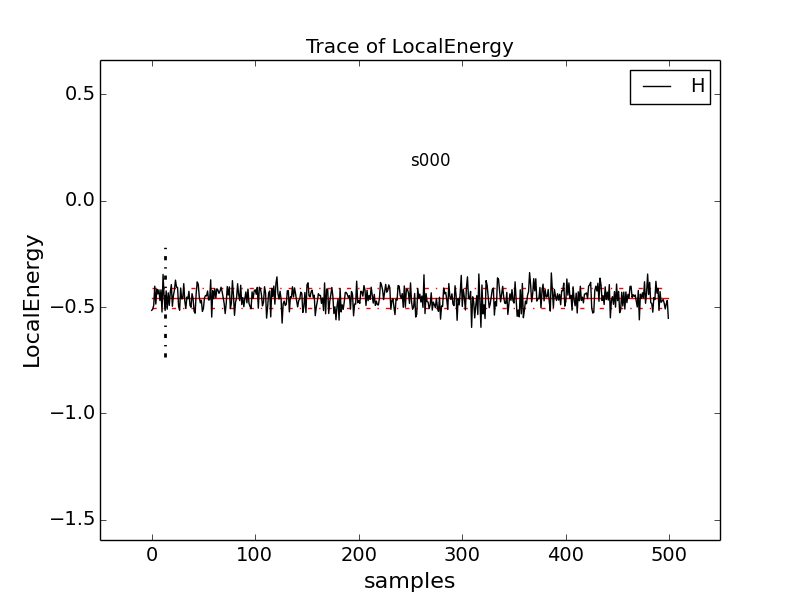
\includegraphics[trim = 0mm 0mm 0mm 0mm, clip,width=0.75\columnwidth]{./figures/lab_qmc_statistics_tracing1.png}
\end{center}
\end{figure}
\FloatBarrier

%\includegraphics[scale=0.5]{E_L_H_STO-2G.png}

The solid black line connects the values of the local energy at each MC block
(labeled ``samples'').  The average value is marked with a horizontal, solid
red line.  One standard deviation above and below the average are marked with
horizontal, dashed red lines.  

The trace of this run is largely centered around the average with no
large-scale oscillations or major shifts, indicating a good quality MC run. 

Try tracing the kinetic and potential energies, seeing that their behavior is
comparable to the total local energy.

Change to directory \texttt{problematic} and type \textbf{qmca -q e -t
H.s000.scalar.dat} to produce this graph:

\FloatBarrier
\begin{figure}[ht!]
\begin{center}
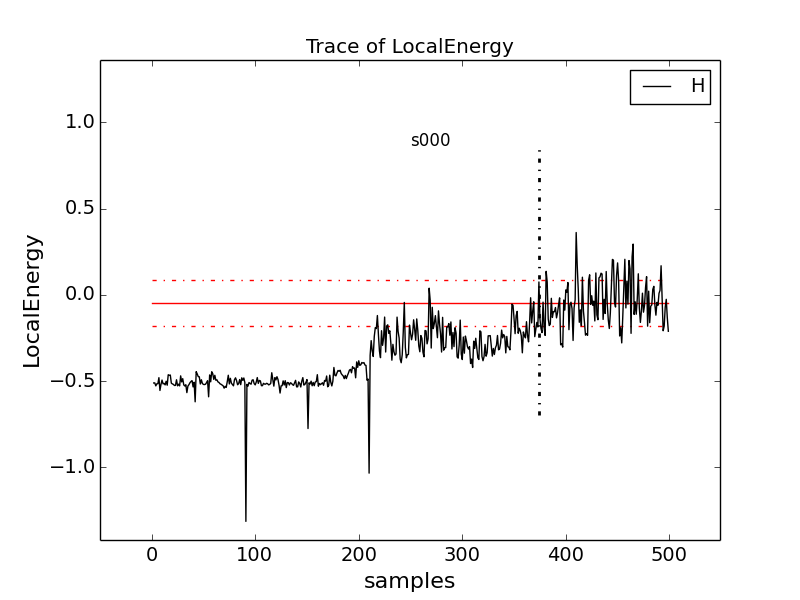
\includegraphics[trim = 0mm 0mm 0mm 0mm, clip,width=0.75\columnwidth]{./figures/lab_qmc_statistics_tracing2.png}
\end{center}
\end{figure}
\FloatBarrier

%\includegraphics[scale=0.5]{E_L_H_B-splines.png}

Here, the local energy samples cluster around the expected -0.5 hartrees for the
first 150 samples or so and then begin to oscillate more wildly and increase
erratically toward 0, indicating a poor quality MC run.

Again, trace the kinetic and potential energies in this run and see how their
behavior compares to the total local energy.

\subsection{Blocking away autocorrelation}

\textit{Autocorrelation} occurs when a given MC step biases subsequent MC
steps, leading to samples that are not statistically independent.  We must take
this autocorrelation into account in order to obtain accurate statistics.  qmca
outputs autocorrelation when given the {-}{-}sac flag.

Change to directory \texttt{autocorrelation} and type \textbf{qmca -q e
{-}{-}sac H.s000.scalar.dat}.  

\begin{shade} 
H  series 0  LocalEnergy = -0.454982 +/- 0.000430    1.0 
\end{shade}

The value after the error bar on the quantity is the autocorrelation (1.0 in
this case).

Proposing too small a step in configuration space, the MC \textit{time step},
can lead to autocorrelation since the new samples will be in the neighborhood
of previous samples.  Type \textbf{grep timestep H.xml} to see the varying time
step values in this QMCPACK input file (H.xml):

\begin{shade} 
<parameter name="timestep">10</parameter>
<parameter name="timestep">5</parameter> 
<parameter name="timestep">2</parameter> 
<parameter name="timestep">1</parameter>
<parameter name="timestep">0.5</parameter> 
<parameter name="timestep">0.2</parameter> 
<parameter name="timestep">0.1</parameter>
<parameter name="timestep">0.05</parameter> 
<parameter name="timestep">0.02</parameter> 
<parameter name="timestep">0.01</parameter>
<parameter name="timestep">0.005</parameter> 
<parameter name="timestep">0.002</parameter> 
<parameter name="timestep">0.001</parameter>
<parameter name="timestep">0.0005</parameter> 
<parameter name="timestep">0.0002</parameter> 
<parameter name="timestep">0.0001</parameter> 
\end{shade}

Generally, as the time step decreases, the autocorrelation will increase
(caveat: very large time steps will also have increasing autocorrelation). To
see this, type \textbf{qmca -q e {-}{-}sac *.scalar.dat} to see the energies
and autocorrelation times, then plot with gnuplot by inputting \textbf{gnuplot
H.plt}:

\FloatBarrier
\begin{figure}[ht!]
\begin{center}
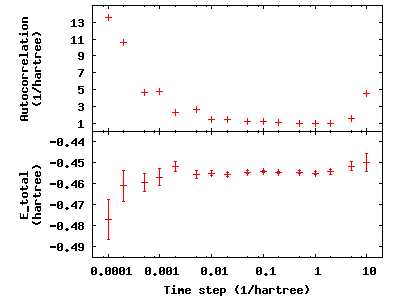
\includegraphics[trim = 0mm 0mm 0mm 0mm, clip,width=0.75\columnwidth]{./figures/lab_qmc_statistics_blocking1.png}
\end{center}
\end{figure}
\FloatBarrier

%\includegraphics[scale=1.0]{timestep_vs_autocorrelation_energy_H_STO-2G.png}

The error bar also increases with the autocorrelation.  

Press \textbf{q [Enter]} to quit gnuplot.

To get around the bias of autocorrelation, we group the MC steps into blocks,
take the average of the data in the steps of each block, and then finally
average the averages in all the blocks.  QMCPACK outputs the block averages as
each line in the scalar.dat file.  (For DMC simulations, in addition to the
scalar.dat, QMCPACK outputs the quantities at each step to the dmc.dat file,
which permits reblocking the data differently from the specification in the
input file.) 

Change directories to \texttt{blocking}.  Here we look at the time step of the
last data set in the \texttt{autocorrelation} directory.  Verify this by typing
\textbf{grep timestep H.xml} to see that all values are set to 0.001.  Now to
see how we will vary the blocking, type \textbf{grep -A1 blocks H.xml}.  The
parameter ``steps'' indicates the number of steps per block, and the parameter
``blocks'' gives the number of blocks.  For this comparison, the total number
of MC steps (equal to the product of ``steps'' and ``blocks'') is fixed at
50000.  Now check the effect of blocking on autocorrelation--type \textbf{qmca
-q e {-}{-}sac *scalar.dat} to see the data and \textbf{gnuplot H.plt} to
visualize the data:

%\begin{shaded} 
%\begin{verbatim} 
%H  series 0  LocalEnergy = -0.454433 +/- 0.003970   189.2 
%H  series 1  LocalEnergy = -0.453352 +/- 0.004159   104.5 
%H  series 2  LocalEnergy = -0.449211 +/- 0.006544   114.1 
%H  series 3  LocalEnergy = -0.449491 +/- 0.014770   381.1 
%H  series 4  LocalEnergy = -0.446602 +/- 0.008809   78.2 
%H  series 5  LocalEnergy = -0.488471 +/- 0.006704   27.2 
%H  series 6  LocalEnergy = -0.427345 +/- 0.011377   50.0 
%H  series 7  LocalEnergy = -0.456044 +/- 0.014513   51.1 
%H  series 8  LocalEnergy = -0.453782 +/- 0.016594   24.1 
%H  series 9  LocalEnergy = -0.482306 +/- 0.028252   21.6 
%H  series 10  LocalEnergy = -0.405258 +/- 0.013696   22.4 
%H  series 11  LocalEnergy = -0.423111 +/- 0.003579    2.9 
%H  series 12  LocalEnergy = -0.474759 +/- 0.016879    9.6 
%H  series 13  LocalEnergy = -0.414045 +/- 0.003606    5.5 
%H  series 14  LocalEnergy = -0.432808 +/- 0.004773    3.3 
%H  series 15  LocalEnergy = -0.465723 +/- 0.004425    2.6 
%\end{verbatim}
%\end{shaded}

\FloatBarrier
\begin{figure}[ht!]
\begin{center}
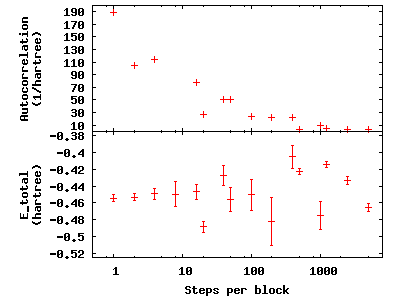
\includegraphics[trim = 0mm 0mm 0mm 0mm, clip,width=0.75\columnwidth]{./figures/lab_qmc_statistics_blocking2.png}
\end{center}
\end{figure}
\FloatBarrier

%\includegraphics[scale=1.0]{steps_per_block_vs_autocorrelation_energy_H_STO-2G.png}

The greatest number of steps per block produces the smallest autocorrelation
time.  The larger number of blocks over which to average at small
step-per-block number masks the corresponding increase in error bar with
increasing autocorrelation.

Press \textbf{q [Enter]} to quit gnuplot.

\subsection{Balancing autocorrelation and acceptance ratio}

Adjusting the time step value also affects the ratio of accepted steps to
proposed steps.  Stepping nearby in configuration space implies that the
probability distribution is similar and thus more likely to result in an
accepted move.  Keeping the acceptance ratio high means the algorithm is
efficiently exploring configuration space and not sticking at particular
configurations.  Return to the \ishell{autocorrelation} directory.  Refresh your
memory on the time steps in this set of simulations by \textbf{grep timestep
H.xml}. Then, type \textbf{qmca -q ar *scalar.dat} to see the acceptance ratio
as it varies with decreasing time step:

\begin{shade} 
H  series 0  AcceptRatio = 0.047646 +/- 0.000206 
H  series 1  AcceptRatio = 0.125361 +/- 0.000308 
H  series 2  AcceptRatio = 0.328590 +/- 0.000340 
H  series 3  AcceptRatio = 0.535708 +/- 0.000313 
H  series 4  AcceptRatio = 0.732537 +/- 0.000234 
H  series 5  AcceptRatio = 0.903498 +/- 0.000156 
H  series 6  AcceptRatio = 0.961506 +/- 0.000083 
H  series 7  AcceptRatio = 0.985499 +/- 0.000051 
H  series 8  AcceptRatio = 0.996251 +/- 0.000025 
H  series 9  AcceptRatio = 0.998638 +/- 0.000014 
H  series 10  AcceptRatio = 0.999515 +/- 0.000009 
H  series 11  AcceptRatio = 0.999884 +/- 0.000004 
H  series 12  AcceptRatio = 0.999958 +/- 0.000003 
H  series 13  AcceptRatio = 0.999986 +/- 0.000002 
H  series 14  AcceptRatio = 0.999995 +/- 0.000001 
H  series 15  AcceptRatio = 0.999999 +/- 0.000000 
\end{shade}

By series 8 (time step = 0.02), the acceptance ratio is in excess of 99\%.  

Considering the increase in autocorrelation and subsequent increase in error
bar as time step decreases, it is important to choose a time step that trades
off appropriately between acceptance ratio and autocorrelation.  In this
example, a time step of 0.02 occupies a spot where acceptance ratio is high
(99.6\%), and autocorrelation is not appreciably larger than the minimum value
(1.4 vs. 1.0).

\subsection{Considering variance}

Besides autocorrelation, the dominant contributor to the error bar is the
\textit{variance} in the local energy.  The variance measures the fluctuations
around the average local energy, and, as the fluctuations go to zero, the wave
function reaches an exact eigenstate of the Hamiltonian.  qmca calculates this
from the local energy and local energy squared columns of the scalar.dat. 

Type \textbf{qmca -q v H.s009.scalar.dat} to calculate the variance on the run
with time step balancing autocorrelation and acceptance ratio:

\begin{shade}
H  series 9  Variance = 0.513570 +/- 0.010589  
\end{shade}

Just as the total energy doesn't tell us much by itself, neither does the
variance.  However, comparing the ratio of the variance to the energy indicates
how the magnitude of the fluctuations compares to the energy itself.   Type
\textbf{qmca -q ev H.s009.scalar.dat} to calculate the energy and variance on
the run side by side with the ratio:

\begin{shade}
                     LocalEnergy               Variance        ratio
H  series 0  -0.454460 +/- 0.000568   0.529496 +/- 0.018445   1.1651
\end{shade}

1.1651 is a very high ratio indicating the square of the fluctuations is on
average larger than the value itself.  In the next section, we will approach
ways to improve the variance that subsequent labs will build upon.  

\section{Reducing statistical error bars}

\subsection{Increasing MC sampling}

Increasing the number of MC samples in a data set reduces the error bar as the
inverse of the square root of the number of samples.  There are two ways to
increase the number of MC samples in a simulation: running more samples in
parallel and increasing the number of blocks (with fixed number of steps per
block, this increases the total number of MC steps).

To see the effect of the running more samples in parallel, change to the
directory \ishell{nodes}.  The series here increases the number of nodes by
factors of four from 32 to 128 to 512.  Type \textbf{qmca -q ev *scalar.dat}
and note the change in the error bar on the local energy as the number of
nodes.  Visualize this with \textbf{gnuplot H.plt}:

\FloatBarrier
\begin{figure}[ht!]
\begin{center}
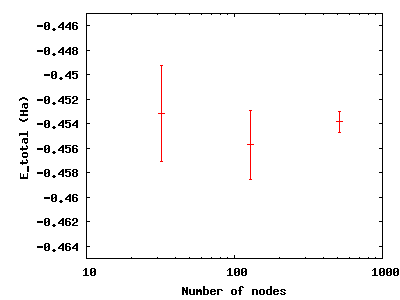
\includegraphics[trim = 0mm 0mm 0mm 0mm, clip,width=0.75\columnwidth]{./figures/lab_qmc_statistics_nodes.png}
\end{center}
\end{figure}
\FloatBarrier

%\includegraphics[scale=1.0]{nnode_vs_energy_H_STO-2G.png}

Increasing the number of blocks, unlike running in parallel, increases the
total CPU time of the simulation.  

Press \textbf{q [Enter]} to quit gnuplot.

To see the effect of increasing the block number, change to the directory
\ishell{blocks}. To see how we will vary the number of blocks, type
\textbf{grep -A1 blocks H.xml}.  The number of steps remains fixed, thus
increasing the total number of samples.   Visualize the tradeoff by inputting
\textbf{gnuplot H.plt}: 

\FloatBarrier
\begin{figure}[ht!]
\begin{center}
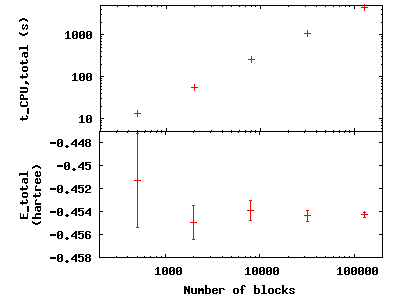
\includegraphics[trim = 0mm 0mm 0mm 0mm, clip,width=0.75\columnwidth]{./figures/lab_qmc_statistics_blocks.png}
\end{center}
\end{figure}
\FloatBarrier

%\includegraphics[scale=1.0]{nblock_vs_tcpu_energy_H_STO-2G.png}

Press \textbf{q [Enter]} to quit gnuplot.

\subsection{Improving the basis set}

In all of the above examples, we are using the sum of two gaussian functions
(STO-2G) to approximate what should be a simple decaying exponential (STO =
Slater-type orbital) for the wave function of the ground state of the hydrogen
atom.  The sum of multiple copies of a function varying each copy's width and
amplitude with coefficients is called a \textit{basis set}. As we add gaussians
to the basis set, the approximation improves, the variance goes toward zero and
the energy goes to -0.5 hartrees.  In nearly every other case, the exact
function is unknown, and we add basis functions until the total energy does not
change within some threshold.

Change to the directory \ishell{basis} and look at the total energy and
variance as we change the wave function by typing \textbf{qmca -q ev H\_*}:

\begin{shade}
                            LocalEnergy               Variance        ratio 
H_STO-2G  series 0  -0.454460 +/- 0.000568   0.529496 +/- 0.018445   1.1651 
H_STO-3G  series 0  -0.465386 +/- 0.000502   0.410491 +/- 0.010051   0.8820 
H_STO-6G  series 0  -0.471332 +/- 0.000491   0.213919 +/- 0.012954   0.4539 
H__exact  series 0  -0.500000 +/- 0.000000   0.000000 +/- 0.000000   -0.0000 
\end{shade}

qmca also puts out the ratio of the variance to the local energy in a column to
the right of the variance error bar.  A typical high quality value for this
ratio is lower than 0.1 or so--none of these few-gaussian wave functions
satisfy that rule of thumb.

Use qmca to plot the trace of the local energy, kinetic energy, and potential
energy of H\_\_exact--the total energy is constantly -0.5 hartree even though
the kinetic and potential energies fluctuate from configuration to
configuration.

\subsection{Adding a Jastrow factor}

Another route to reducing the variance is the introduction of a Jastrow factor to 
account for electron-electron correlation (not the statistical autocorrelation
of Monte Carlo steps but the physical avoidance that electrons have of one another).
To do this, we will switch to the hydrogen dimer with the exact ground state
wave function of the atom (STO basis)--this will not be exact for the dimer.
The ground state energy of the hydrogen dimer is -1.174 hartrees.

Change directories to \ishell{dimer} and put in \textbf{qmca -q ev *scalar.dat}
to see the result of adding a simple, one-parameter Jastrow to the STO basis
for the hydrogen dimer at experimental bond length:

\begin{shade}
                               LocalEnergy               Variance           
H2_STO___no_jastrow  series 0  -0.876548 +/- 0.005313   0.473526 +/- 0.014910
H2_STO_with_jastrow  series 0  -0.912763 +/- 0.004470   0.279651 +/- 0.016405
\end{shade}

The energy reduces by 0.044 +/- 0.006 hartrees and the variance by 0.19 +/- 0.02.
This is still 20\% above the ground state energy, and subsequent labs will cover how
to improve on this with improved forms of the wave function that capture more
of the physics.

\section{Scaling to larger numbers of electrons}

\subsection{Calculating the efficiency}

The inverse of the product of CPU time and the variance measures the
\textit{efficiency} of an MC calculation.  Use qmca to calculate efficiency by
typing \textbf{qmca -q eff *scalar.dat} to see the efficiency of these two
H$_2$ calculations:

\begin{shade}
H2_STO___no_jastrow  series 0  Efficiency = 16698.725453 +/- 0.000000 
H2_STO_with_jastrow  series 0  Efficiency = 52912.365609 +/- 0.000000 
\end{shade}

The Jastrow factor increased the efficiency in these calculations by a factor
of three, largely through the reduction in variance (check the average block
CPU time to verify this claim).

\subsection{Scaling up}

To see how MC scales with increasing particle number, change directories to
\ishell{size}.  Here are the data from runs of increasing number of electrons
for H, H$_2$, C, CH$_4$, C$_2$, C$_2$H$_4$, (CH$_4$)$_2$, and (C$_2$H$_4$)$_2$
using the STO-6G basis set for the orbitals of the Slater determinant.  The file names begin with the number of electrons simulated for those data.

Use \textbf{qmca -q bc *scalar.dat} to see that the CPU time per block
increases with number of electrons in the simulation, then plot the total CPU
time of the simulation by \textbf{gnuplot Nelectron\_tCPU.plt}:

\FloatBarrier
\begin{figure}[ht!]
\begin{center}
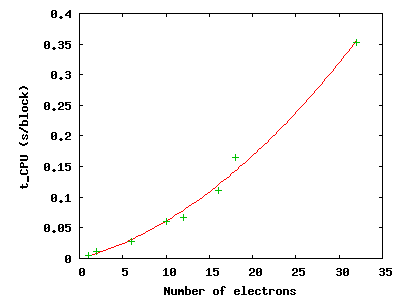
\includegraphics[trim = 0mm 0mm 0mm 0mm, clip,width=0.75\columnwidth]{./figures/lab_qmc_statistics_scaling.png}
\end{center}
\end{figure}
\FloatBarrier

%\includegraphics[scale=1.0]{nelectron_vs_tcpu_H_C_CH_STO-6G.png}

The green pluses represent the CPU time per block at each electron number.
The red line is a quadratic fit to those data.  For a fixed basis set size, we expect the time to scale quadratically up to 1000s of electrons, at which point a cubic scaling term may become dominant.  Knowing the scaling allows you to roughly project the calculation time for a larger number of electrons.

Press \textbf{q [Enter]} to quit gnuplot.

This isn't the whole story, however.  The variance of the energy also increases
with a fixed basis set as the number of particles increases at a faster rate
than the energy decreases.  To see this, type \textbf{qmca -q ev *scalar.dat}:

\begin{shade}
                            LocalEnergy               Variance           
01________H  series 0  -0.471352 +/- 0.000493      0.213020 +/- 0.012950 
02_______H2  series 0  -0.898875 +/- 0.000998      0.545717 +/- 0.009980 
06________C  series 0  -37.608586 +/- 0.020453   184.322000 +/- 45.481193
10______CH4  series 0  -38.821513 +/- 0.022740   169.797871 +/- 24.765674
12_______C2  series 0  -72.302390 +/- 0.037691   491.416711 +/- 106.090103
16_____C2H4  series 0  -75.488701 +/- 0.042919   404.218115 +/- 60.196642
18___CH4CH4  series 0  -58.459857 +/- 0.039309   498.579645 +/- 92.480126
32_C2H4C2H4  series 0  -91.567283 +/- 0.048392   632.114026 +/- 69.637760
\end{shade}

The increase in variance is not uniform, but the general trend is upward with a
fixed wave function form and basis set.  Subsequent labs will address how to
improve the wave function in order to keep the variance manageable.

\chapter{Lab 2: QMC Basics}
\label{chap:lab_qmc_basics}



\section{Topics covered in this Lab}
This lab focuses on the basics of performing quality QMC calculations.  As an example participants test an oxygen pseudopotential within DMC by calculating atomic and dimer properties, a common step prior to production runs.  Topics covered include:
\begin{itemize}
  \item{converting pseudopotentials into QMCPACK's FSATOM format}
  \item{generating orbitals with Quantum ESPRESSO}
  \item{converting orbitals into QMCPACK's ESHDF format with pw2qmcpack}
  \item{optimizing Jastrow factors with QMCPACK}
  \item{removing DMC timestep error via extrapolation}
  \item{automating QMC workflows with Nexus}
  \item{testing pseudopotentials for accuracy}
  \hide{
  \item{(optional) running QMCPACK for a general system of interest}
  }
\end{itemize}

\section{Lab outline}
\begin{enumerate}
  \item{download and conversion of oxygen atom pseudopotential}
  \item{DMC timestep study of the neutral oxygen atom}
  \begin{enumerate}
    \item{DFT orbital generation with Quantum ESPRESSO}
    \item{orbital conversion with \ishell{pw2qmcpack.x}}
    \item{optimization of Jastrow correlation factor with QMCPACK}
    \item{DMC run with multiple timesteps}
  \end{enumerate}
  \item{DMC timestep study of the first ionization potential of oxygen}
  \begin{enumerate}
    \item{repetition of a-d above for ionized oxygen atom}
  \end{enumerate}
  \item{automated DMC calculations of the oxygen dimer binding curve}
\end{enumerate}


\section{Lab directories and files}
\footnotesize
\begin{verbatim}%
labs/lab2_qmc_basics/
│
├── oxygen_atom           - oxygen atom calculations 
│   ├── O.q0.dft.in          - Quantum ESPRESSO input for DFT run
│   ├── O.q0.p2q.in          - pw2qmcpack.x input for orbital conversion run
│   ├── O.q0.opt.in.xml      - QMCPACK input for Jastrow optimization run
│   ├── O.q0.dmc.in.xml      - QMCPACK input file for neutral O DMC
│   ├── ip_conv.py           - tool to fit oxygen IP vs timestep
│   └── reference            - directory w/ completed runs
│
├── oxygen_dimer          - oxygen dimer calculations
│   ├── dimer_fit.py         - tool to fit dimer binding curve
│   ├── O_dimer.py           - automation script for dimer calculations
│   ├── pseudopotentials     - directory for pseudopotentials
│   └── reference            - directory w/ completed runs
│
└── your_system           - performing calculations for an arbitrary system (yours)
    ├── example.py           - example nexus file for periodic diamond
    ├── pseudopotentials     - directory containing C pseudopotentials
    └── reference            - directory w/ completed runs
\end{verbatim}
\normalsize

\section{Obtaining and converting a pseudopotential for oxygen}
\label{sec:lqb_pseudo}
First enter the \ishell{oxygen\_atom} directory:
\begin{shade}
cd labs/lab2_qmc_basics/oxygen_atom/
\end{shade}
\noindent
Throughout the rest of the lab, locations will be specified with respect to \ishell{labs/lab2\_qmc\_basics} (e.g. \ishell{oxygen\_atom}).

We will use a potential from the Burkatzki-Filippi-Dolg pseudopotential database.  
Although the full database is available in QMCPACK distribution (\ishell{trunk/pseudopotentials/BFD/}), 
we use a BFD pseudopotential to illustrate the process of converting and testing an 
external potential for use with QMCPACK.   To obtain the pseudopotential, go to 
\href{http://www.burkatzki.com/pseudos/index.2.html}{http://www.burkatzki.com/pseudos/index.2.html}
and click on the ``Select Pseudopotential'' button.  Next click on oxygen in the 
periodic table.  Click on the empty circle next to ``V5Z'' (a large gaussian 
basis set) and click on ``Next''.  Select the Gamess format and click on 
``Retrive Potential''.  Helpful information about the pseudopotential will be 
displayed.  The desired portion is at the bottom (the last 7 lines).  Copy 
this text into the editor of your choice (e.g. \ishell{emacs} or \ishell{vi}) 
and save it as \ishell{O.BFD.gamess} 
(be sure to include a newline at the end of the file).  To transform the 
pseudopotential into the FSATOM XML format used by QMCPACK, use the \ishell{ppconvert} 
tool:

\noindent
\ifws
\begin{shade}
ppconvert --gamess_pot O.BFD.gamess --s_ref "1s(2)2p(4)" \
 --p_ref "1s(2)2p(4)" --d_ref "1s(2)2p(4)" --xml O.BFD.xml
\end{shade}
\else
\begin{shade}
jobrun_vesta ppconvert --gamess_pot O.BFD.gamess --s_ref "1s(2)2p(4)" \
 --p_ref "1s(2)2p(4)" --d_ref "1s(2)2p(4)" --xml O.BFD.xml
\end{shade}
\fi

\noindent
Observe the notation used to describe the reference valence configuration for this helium-core PP: \ishell{1s(2)2p(4)}.  The \ishell{ppconvert} tool uses the following convention for the valence states: the first $s$ state is labeled \ishell{1s} (\ishell{1s}, \ishell{2s}, \ishell{3s}, \ldots), the first $p$ state is labeled \ishell{2p} (\ishell{2p}, \ishell{3p}, \ldots), the first $d$ state is labeled \ishell{3d} (\ishell{3d}, \ishell{4d}, \ldots). Copy the resulting xml file into the \ishell{oxygen\_atom} directory.

Note: the command to convert the PP into QM Espresso's UPF format is similar (both formats are required):

\noindent
\ifws
\begin{shade}
ppconvert --gamess_pot O.BFD.gamess --s_ref "1s(2)2p(4)" \
 --p_ref "1s(2)2p(4)" --d_ref "1s(2)2p(4)" --log_grid --upf O.BFD.upf
\end{shade}
\else
\begin{shade}
jobrun_vesta ppconvert --gamess_pot O.BFD.gamess --s_ref "1s(2)2p(4)" \
 --p_ref "1s(2)2p(4)" --d_ref "1s(2)2p(4)" --log_grid --upf O.BFD.upf
\end{shade}
\noindent
\fi

For reference, the text of \ishell{O.BFD.gamess} should be:
\begin{lstlisting}
O-QMC GEN 2 1
3
6.00000000 1 9.29793903
55.78763416 3 8.86492204
-38.81978498 2 8.62925665
1
38.41914135 2 8.71924452

\end{lstlisting}
\noindent
The full QMCPACK pseudopotential is also included in \ishell{oxygen\_atom/reference/O.BFD.*}.


\section{DFT with Quantum ESPRESSO to obtain the orbital part of the wavefunction}
\label{sec:lqb_dft}
With the pseudopotential in hand, the next step toward a QMC calculation is to obtain the Fermionic part of the wavefunction, in this case a single Slater determinant constructed from DFT-LDA orbitals for a neutral oxygen atom.  If you had trouble with the pseudopotential conversion step, pre-converted pseudopotential files are located in the \ishell{oxygen\_atom/reference} directory.  

Quantum ESPRESSO input for the DFT-LDA ground state of the neutral oxygen atom can be found in \ishell{O.q0.dft.in} and also listing \ref{lst:O_q0_dft} below.  Setting \ishell{wf\_collect=.true.} instructs Quantum Espresso to write the orbitals to disk at the end of the run. Option \ishell{wf\_collect=.true.} may be a potential problem in large simulations, it is recommended to avoid it and use the converter pw2qmcpack in parallel, see details in Sec.~\ref{sec:pw2qmcpack}. Note that the plane-wave energy cutoff has been set to a reasonable value of 300 Ry here (\ishell{ecutwfc=300}).  This value depends on the pseudopotentials used, and in general should be selected by running DFT$\rightarrow$(orbital conversion)$\rightarrow$VMC with increasing energy cutoffs until the lowest VMC total energy and variance is reached.

\begin{lstlisting}[style=ESPRESSO, language=espresso, caption={Quantum ESPRESSO input file for the neutral oxygen atom (\ishell{O.q0.dft.in})\label{lst:O_q0_dft}}]
&CONTROL
   calculation       = 'scf'
   restart_mode      = 'from_scratch'
   prefix            = 'O.q0'
   outdir            = './'
   pseudo_dir        = './'
   disk_io           = 'low'
   wf_collect        = .true.
/

&SYSTEM
   celldm(1)         = 1.0
   ibrav             = 0
   nat               = 1
   ntyp              = 1
   nspin             = 2
   tot_charge        = 0
   tot_magnetization = 2
   input_dft         = 'lda'
   ecutwfc           = 300
   ecutrho           = 1200
   nosym             = .true.
   occupations       = 'smearing'
   smearing          = 'fermi-dirac'
   degauss           = 0.0001
/

&ELECTRONS
   diagonalization   = 'david'
   mixing_mode       = 'plain'
   mixing_beta       = 0.7
   conv_thr          = 1e-08
   electron_maxstep  = 1000
/


ATOMIC_SPECIES 
   O  15.999 O.BFD.upf

ATOMIC_POSITIONS alat
   O     9.44863067       9.44863161       9.44863255

K_POINTS automatic
   1 1 1  0 0 0 

CELL_PARAMETERS cubic
        18.89726133       0.00000000       0.00000000 
         0.00000000      18.89726133       0.00000000 
         0.00000000       0.00000000      18.89726133
\end{lstlisting}

Run Quantum ESPRESSO by typing 
\ifws
\begin{shade}
mpirun -np 4 pw.x -input O.q0.dft.in >&O.q0.dft.out&
\end{shade}
\else
\begin{shade}
jobrun_vesta pw.x O.q0.dft.in
\end{shade}
\fi

The DFT run should take a few minutes to complete.  If desired, you can track the progress of the DFT run by typing ``\ifws\ishell{tail -f O.q0.dft.out}
\else\ishell{tail -f O.q0.dft.output}\fi''. Once finished, you should check the LDA total energy in \ifws\ishell{O.q0.dft.out}\else\ishell{O.q0.dft.output}\fi by typing ``\ifws\ishell{grep '!  ' O.q0.dft.out}\else\ishell{grep '!  ' O.q0.dft.output}\fi''.  The result should be close to
\begin{shade}
!    total energy              =     -31.57553905 Ry
\end{shade} 
% both of the numbers below are for 200 Ry (too small as it turns out)
% 10 Angstrom cell
%!    total energy              =     -31.56729415 Ry
% 15 Angstrom cell
%!    total energy              =     -31.56730213 Ry



The orbitals have been written in a format native to Quantum ESPRESSO in the \ishell{O.q0.save} directory.  We will convert them into the ESHDF format expected by QMCPACK by using the \ishell{pw2qmcpack.x} tool.  The input for \ishell{pw2qmcpack.x} can be found in the file \ishell{O.q0.p2q.in} and also in listing \ref{lst:O_q0_p2q} below. 

\begin{lstlisting}[caption={\ishell{pw2qmcpack.x} input file for orbital conversion (\ishell{O.q0.p2q.in})\label{lst:O_q0_p2q}}]
&inputpp
  prefix     = 'O.q0'
  outdir     = './'
  write_psir = .false.
/
\end{lstlisting}

Perform the orbital conversion now by typing the following:
\ifws
\begin{shade}
mpirun -np 1 pw2qmcpack.x<O.q0.p2q.in>&O.q0.p2q.out&
\end{shade}
\else
\begin{shade}
jobrun_vesta pw2qmcpack.x O.q0.p2q.in
\end{shade}
\fi
\noindent
Upon completion of the run, a new file should be present containing the orbitals for QMCPACK: \ishell{O.q0.pwscf.h5}.  Template XML files for particle (\ishell{O.q0.ptcl.xml}) and wavefunction (\ishell{O.q0.wfs.xml}) inputs to QMCPACK should also be present.  


\section{Optimization with QMCPACK to obtain the correlated part of the wavefunction}\label{sec:optimization_walkthrough}
The wavefunction we have obtained to this point corresponds to a non-interacting Hamiltonian.  Once the Coulomb pair potential is switched on between particles, it is known analytically that the exact wavefunction has cusps whenever two particles meet spatially and in general the electrons become correlated.  This is represented in the wavefunction by introducing a Jastrow factor containing at least pair correlations
\begin{align}
  &\Psi_{Slater-Jastrow}=e^{-J}\Psi_{Slater} \\
  &J = \sum_{\sigma\sigma'}\sum_{i<j}u^{\sigma\sigma'}_2(|r_i-r_j|) + \sum_\sigma\sum_{iI}u^{\sigma I}_1(|r_i-r_I|)
\end{align}
Here $\sigma$ is a spin variable while $r_i$ and $r_I$ represent electron and ion coordinates, respectively.  The introduction of $J$ into the wavefunction is similar to F12 methods in quantum chemistry, though it has been present in essentially all QMC studies since the first applications the method (circa 1965).

How are the functions $u_2^{\sigma\sigma'}$ and $u_1^{\sigma}$ obtained?  Generally, they are approximated by analytical functions with several unknown parameters that are determined by minimizing the energy or variance directly within VMC.  This is effective because the energy and variance reach a global minimum only for the true ground state wavefunction ($\textrm{Energy}=E\equiv\expval{\Psi}{\hat{H}}{\Psi}$, $\textrm{Variance}=V\equiv\expval{\Psi}{(\hat{H}-E)^2}{\Psi}$).  For this exercise, we will focus on minimizing the variance.

% background on the wavefunction should be covered elsewhere in the manual
%   perhaps replace this with just the figure and a couple of brief comments 
\hide{
\subsubsection{Background on trial wavefunction and optimization}\label{sec:opt_background}
The trial wavefunction used to describe the neutral oxygen atom is of the 
standard Slater-Jastrow form:
\begin{align}  
  \Psi_T = e^{-(J_1+J_2)}D^\uparrow(\{\phi_u^\uparrow\}_{u=1}^{N^\uparrow})D^\downarrow(\{\phi_d^\downarrow\}_{d=1}^{N^\uparrow})
\end{align}
The orbitals forming the spin-restricted Slater determinants 
($D^\uparrow/D^\downarrow$) are obtained from DFT or Hartree-Fock (\emph{e.g.} via Quantum ESPRESSO) 
and are fixed.  The ground state of the (pseudo) oxygen atom is spin polarized 
with $N^{\uparrow}=4$ and $N^{\downarrow}=2$.  

The part of the wavefunction we will be optimizing is the Jastrow factor 
($e^{-(J_1+J_2)}$), which in this case includes one- (electron-ion) and two- 
(electron-electron) body correlation functions.  The Jastrow factor is symmetric 
under same-spin electron exchange and does not affect the DMC fixed node 
approximation.  Optimization of the Jastrow factor does, however, improve the 
efficiency of the DMC calculation and reduces additional approximations due to 
non-local pseudopotentials (locality approximation, T-moves).  Note that a three-body 
term ($J_3$) is also available and is often necessary when using pseudopotentials 
for transition metal species or when high accuracy is desired for molecules.  


\begin{figure}
\begin{center}
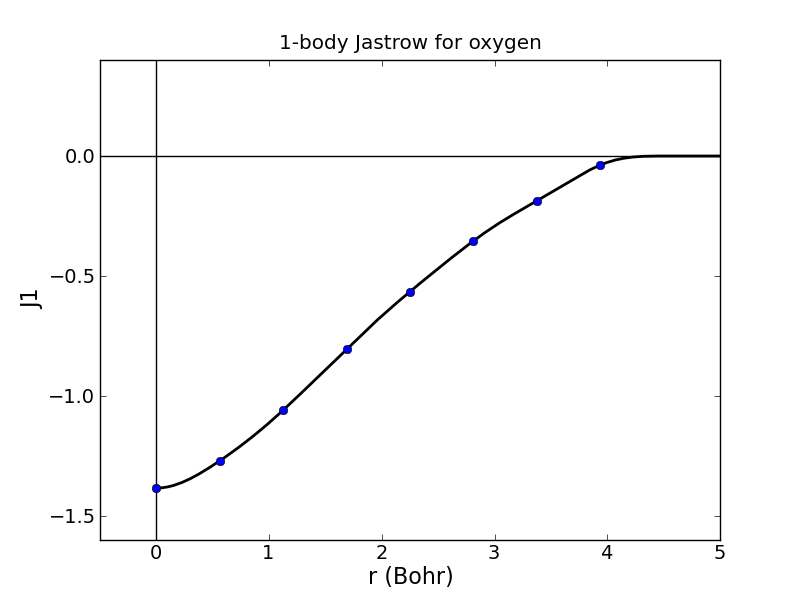
\includegraphics[trim = 0mm 0mm 0mm 0mm, clip,width=0.75\columnwidth]{./figures/lab_qmc_basics_J1.png}
\end{center}
\caption{Optimized $U_1$ function for 1-body Jastrow factor of an oxygen atom.
\label{fig:u1_spline}
}
\end{figure}

The explicit form of the one-body Jastrow factor we will be using is
\begin{align}\label{eq:J1}
  J_1 = \sum_{e=1}^{N^\uparrow+N^\downarrow}U_1^{\uparrow/\downarrow}(|r_e-r_O|)
\end{align}
where $r_e$ refers to the electron positions and $r_O$ is 
the position of the oxygen ion.  The $U_1^{\uparrow/\downarrow}$ term is a 
one-dimensional radial function represented with piecewise continuous cubic 
polynomials (B-splines).  The adjustable parameters to be optimized are the 
``knots'' of the B-splines which are simply the values of the $U_1$ function at 
uniformly spaced grid points (See fig. \ref{fig:u1_spline} for an example of a $U_1$ 
spline function with 8 knots).  

The two-body Jastrow factor is spin resolved ($r^\uparrow/r^\downarrow$ are up/down electron positions):
\begin{align}\label{eq:J2}
  J_2 = \sum_{u<u'}U_2^{\uparrow\uparrow/\downarrow\downarrow}(|r_u^\uparrow-r_{u'}^\uparrow|) + \sum_{d<d'}U_2^{\uparrow\uparrow/\downarrow\downarrow}(|r_d^\downarrow-r_{d'}^\downarrow|) + \sum_{u,d} U_2^{\uparrow\downarrow}(|r_u^\uparrow-r_d^\downarrow|)
\end{align}
For an atom, Pad\'{e} functions are appropriate for $U_2^{\uparrow\uparrow/\downarrow\downarrow}$ and $U_2^{\uparrow\downarrow}$:
\begin{align}
  U_2(r) = \frac{Ar}{1+Br}
\end{align}
Only $B^{\uparrow\uparrow/\downarrow\downarrow}$ and $B^{\uparrow\downarrow}$ are adjustable since the $A$ parameters are fixed by the electron-electron cusp conditions.

Wavefunction optimization essentially relies on two inequalities regarding energy and variance:
\begin{align}
  E_T(P) &= \frac{\expvalh{\Psi_T(P)}{H}{\Psi_T(P)}}{\overlap{\Psi_T(P)}{\Psi_T(P)}} \ge E_0 \\
  V_T(P) &= \frac{\expval{\Psi_T(P)}{\hat{H}^2}{\Psi_T(P)}}{\overlap{\Psi_T(P)}{\Psi_T(P)}} - \left(\frac{\expval{\Psi_T(P)}{H}{\Psi_T(P)}}{\overlap{\Psi_T(P)}{\Psi_T(P)}}\right)^2 \ge 0   
\end{align}
Here $E_0$ is the ground state energy, $E_T(P)$ is the trial energy, $V_T(P)$ is the trial variance, and $P$ denotes the set of adjustable parameters in the trial wavefunction.  Equality is reached only for the true ground state wavefunction and so the trial wavefunction can be improved by attempting to minimize a chosen cost function: 
\begin{align}
  C(P) = \alpha E_T(P) + (1-\alpha) V_T(P).
\end{align}  
Iterative varational Monte Carlo methods have been developed to handle the non-linear optimization problem $\min\limits_P C(P)$.  We will be using the linearized optimization method of Umrigar, \emph{et al.} (PRL \textbf{98} 110201 (2007)).  Let us try this now with QMCPACK.
}

First, we need to update the template particle and wavefunction information in \ishell{O.q0.ptcl.xml} and \ishell{O.q0.wfs.xml}.  We want to simulate the O atom in open boundary conditions (the default is periodic).  To do this open \ishell{O.q0.ptcl.xml} with your favorite text editor (e.g. \ishell{emacs} or \ishell{vi}) and replace
\begin{lstlisting}[style=QMCPXML]
<parameter name="bconds">
   p p p
</parameter>
<parameter name="LR_dim_cutoff">
   15
</parameter>
\end{lstlisting}
with
\begin{lstlisting}[style=QMCPXML]
<parameter name="bconds">
   n n n 
</parameter>
\end{lstlisting}

Next we will select Jastrow factors appropriate for an atom.  In open boundary conditions, the B-spline Jastrow correlation functions should cut off to zero at some distance away from the atom.  Open \ishell{O.q0.wfs.xml} and add the following cutoffs (\ishell{rcut} in Bohr radii) to the correlation factors:
\begin{lstlisting}[style=QMCPXML]
...
<correlation speciesA="u" speciesB="u" size="8" rcut="10.0">
...
<correlation speciesA="u" speciesB="d" size="8" rcut="10.0">
...
<correlation elementType="O" size="8" rcut="5.0">
...
\end{lstlisting}
\noindent
These terms correspond to $u_2^{\uparrow\uparrow}/u_2^{\downarrow\downarrow}$, $u_2^{\uparrow\downarrow}$, and $u_1^{\uparrow O}/u_1^{\downarrow O}$, respectively.  In each case, the correlation function ($u_*$) is represented by piecewise continuous cubic B-splines.  Each correlation function has eight parameters which are just the values of $u$ on a uniformly spaced grid up to \ishell{rcut}.  Initially the parameters (\ishell{coefficients}) are set to zero:
\begin{lstlisting}[style=QMCPXML]
<correlation speciesA="u" speciesB="u" size="8" rcut="10.0">
  <coefficients id="uu" type="Array">
     0.0 0.0 0.0 0.0 0.0 0.0 0.0 0.0
  </coefficients>
</correlation>
\end{lstlisting}

Finally, we need to assemble particle, wavefunction, and pseudopotential information into the main QMCPACK input file (\ishell{O.q0.opt.in.xml}) and specify inputs for the Jastrow optimization process.  Open \ishell{O.q0.opt.in.xml} and write in the location of the particle, wavefunction, and pseudopotential files (``\ishell{<!-- ... -->}'' are comments):
\begin{lstlisting}[style=QMCPXML]
...
<!-- include simulationcell and particle information from pw2qmcpqack -->
<include href="O.q0.ptcl.xml"/>
...
<!-- include wavefunction information from pw2qmcpqack -->
<include href="O.q0.wfs.xml"/>
...
<!-- O pseudopotential read from "O.BFD.xml" -->
<pseudo elementType="O" href="O.BFD.xml"/>
...
\end{lstlisting}
\noindent
The relevant portion of the input describing the linear optimization process is
\begin{lstlisting}[style=QMCPXML]
<loop max="MAX">  
  <qmc method="linear" move="pbyp" checkpoint="-1">
    <cost name="energy"              >  ECOST    </cost>
    <cost name="unreweightedvariance">  UVCOST   </cost>
    <cost name="reweightedvariance"  >  RVCOST   </cost>
    <parameter name="timestep"       >  TS       </parameter>
    <parameter name="samples"        >  SAMPLES  </parameter>
    <parameter name="warmupSteps"    >  50       </parameter>
    <parameter name="blocks"         >  200      </parameter>
    <parameter name="subSteps"       >  1        </parameter>
    <parameter name="nonlocalpp"     >  yes      </parameter>
    <parameter name="useBuffer"      >  yes      </parameter>
    ...
  </qmc>
</loop>
\end{lstlisting}
\noindent
An explanation of each input variable can be found below.  The remaining variables control specialized internal details of the linear optimization algorithm.  The meaning of these inputs is beyond the scope of this lab and reasonable results are often obtained keeping these values fixed. 
\begin{description}
  \item[energy] Fraction of trial energy in the cost function.
  \item[unreweightedvariance] Fraction of unreweighted trial variance in the cost function.  Neglecting the weights can be more robust.
  \item[reweightedvariance] Fraction of trial variance (including the full weights) in the cost function.  
  \item[timestep] Timestep of the VMC random walk, determines spatial distance moved by each electron during MC steps.  Should be chosen such that the acceptance ratio of MC moves is around 50\% (30-70\% is often acceptable).  Reasonable values are often between 0.2 and 0.6 $\textrm{Ha}^{-1}$.
  \item[samples] Total number of MC samples collected for optimization, determines statistical error bar of cost function.  Often efficient to start with a modest number of samples (50k) and then increase as needed.  More samples may be required if the wavefunction contains a large number of variational parameters.  MUST be be a multiple of the number of threads/cores \labsw{}{(use multiples of 512 on Vesta)}.
  \item[warmupSteps]  Number of MC steps discarded as a warmup or equilibration period of the random walk.  If this is too small, it will bias the optimization procedure.
  \item[blocks]  Number of average energy values written to output files.  Should be greater than 200 for meaningful statistical analysis of output data (\emph{e.g.} via \ishell{qmca}).
  \item[subSteps] Number of MC steps in between energy evaluations.  Each energy evaluation is expensive so taking a few steps to decorrelate between measurements can be more efficient.  Will be less efficient with many substeps.
  \item[nonlocalpp,useBuffer] If \ishell{nonlocalpp="no"}, then nonlocal part of the pseudopotential is not included when computing the cost function.  If \ishell{useBuffer="yes"}, then temporary data is stored to speed up nonlocal pseudopotential evaluation at the expense of memory consumption.  
  \item[loop max] Number of times to repeat the optimization.  Using the resulting wavefunction from the previous optimization in the next one improves the results.  Typical choices range between 8 and 16.   
\end{description}
The cost function defines the quantity to be minimized during optimization. The three components of the cost function, energy, unreweighted variance, and reweighted variance should sum to one.  Dedicating 100\% of the cost function to unreweighted variance is often a good choice.  Another common choice is to try 90/10 or 80/20 mixtures of reweighted variance and energy.  Using 100\% energy minimization is desirable for reducing DMC pseudopotential localization errors, but the optimization process is less stable and should only be attempted after performing several cycles of e.g. variance minimization first (the entire \ishell{loop} section can be duplicated with a different cost function each time).

Replace \ishell{MAX}, \ishell{EVCOST}, \ishell{UVCOST}, \ishell{RVCOST}, \ishell{TS}, and \ishell{SAMPLES} in the \ishell{loop} with appropriate starting values in the \ishell{O.q0.opt.in.xml} input file.  Perform the optimization run by typing
\ifws
\begin{shade}
mpirun -np 4 qmcpack O.q0.opt.in.xml >&O.q0.opt.out&
\end{shade}
\else
\begin{shade}
jobrun_vesta qmcpack O.q0.opt.in.xml
\end{shade}
\fi
\noindent
The run should only take a few minutes for reasonable values of loop \ishell{max} and \ishell{samples}.  

Log file output will appear in \labsw{\ishell{O.q0.opt.out}}{\ishell{O.q0.opt.output}}.  The beginning of each linear optimization will be marked with text similar to
\begin{shade}
=========================================================
  Start QMCFixedSampleLinearOptimize
  File Root O.q0.opt.s011 append = no 
=========================================================
\end{shade}
\noindent
At the end of each optimization section the change in cost function, new values for the Jastrow parameters, and elapsed wallclock time are reported:
\begin{shade}
 OldCost: 7.0598901869e-01 NewCost: 7.0592576381e-01 Delta Cost:-6.3254886314e-05
...
  <optVariables href="O.q0.opt.s011.opt.xml">
uu_0 6.9392504232e-01 1 1  ON 0
uu_1 4.9690781460e-01 1 1  ON 1
uu_2 4.0934542375e-01 1 1  ON 2
uu_3 3.7875640157e-01 1 1  ON 3
uu_4 3.7308380014e-01 1 1  ON 4
uu_5 3.5419786809e-01 1 1  ON 5
uu_6 4.3139019377e-01 1 1  ON 6
uu_7 1.9344371667e-01 1 1  ON 7
ud_0 3.9219009713e-01 1 1  ON 8
ud_1 1.2352664647e-01 1 1  ON 9
ud_2 4.4048945133e-02 1 1  ON 10
ud_3 2.1415676741e-02 1 1  ON 11
ud_4 1.5201803731e-02 1 1  ON 12
ud_5 2.3708169445e-02 1 1  ON 13
ud_6 3.4279064930e-02 1 1  ON 14
ud_7 4.3334583596e-02 1 1  ON 15
eO_0 -7.8490123937e-01 1 1  ON 16
eO_1 -6.6726618338e-01 1 1  ON 17
eO_2 -4.8753453838e-01 1 1  ON 18
eO_3 -3.0913993774e-01 1 1  ON 19
eO_4 -1.7901872177e-01 1 1  ON 20
eO_5 -8.6199000697e-02 1 1  ON 21
eO_6 -4.0601160841e-02 1 1  ON 22
eO_7 -4.1358075061e-03 1 1  ON 23
  </optVariables>
...
  QMC Execution time = 2.8218972974e+01 secs
\end{shade}
\noindent
The cost function should decrease during each linear optimization (\ishell{Delta cost < 0}).  Try ``\labsw{\ishell{grep OldCost *opt.out}}{\ishell{grep OldCost *opt.output}}''.  You should see something like this:
\begin{shade}
 OldCost: 1.2655186572e+00 NewCost: 7.2443875597e-01 Delta Cost:-5.4107990118e-01
 OldCost: 7.2229830632e-01 NewCost: 6.9833678217e-01 Delta Cost:-2.3961524143e-02
 OldCost: 8.0649629434e-01 NewCost: 8.0551871147e-01 Delta Cost:-9.7758287036e-04
 OldCost: 6.6821241388e-01 NewCost: 6.6797703487e-01 Delta Cost:-2.3537901148e-04
 OldCost: 7.0106275099e-01 NewCost: 7.0078055426e-01 Delta Cost:-2.8219672877e-04
 OldCost: 6.9538522411e-01 NewCost: 6.9419186712e-01 Delta Cost:-1.1933569922e-03
 OldCost: 6.7709626744e-01 NewCost: 6.7501251165e-01 Delta Cost:-2.0837557922e-03
 OldCost: 6.6659923822e-01 NewCost: 6.6651737755e-01 Delta Cost:-8.1860671682e-05
 OldCost: 7.7828995609e-01 NewCost: 7.7735482525e-01 Delta Cost:-9.3513083900e-04
 OldCost: 7.2717974404e-01 NewCost: 7.2715201115e-01 Delta Cost:-2.7732880747e-05
 OldCost: 6.9400639873e-01 NewCost: 6.9257183689e-01 Delta Cost:-1.4345618444e-03
 OldCost: 7.0598901869e-01 NewCost: 7.0592576381e-01 Delta Cost:-6.3254886314e-05
\end{shade}

Blocked averages of energy data, including the kinetic energy and components of the potential energy, are written to \ishell{scalar.dat} files.  The first is named ``\ishell{O.q0.opt.s000.scalar.dat}'', with a series number of zero (\ishell{s000}).  In the end there will be \ishell{MAX} of them, one for each series. 

When the job has finished, use the \ishell{qmca} tool to assess the effectiveness of the optimization process.  To look at just the total energy and the variance, type ``\ishell{qmca -q ev O.q0.opt*scalar*}''.  This will print the energy, variance, and the variance/energy ratio in Hartree units:
\begin{shade}
                            LocalEnergy               Variance           ratio
O.q0.opt  series 0  -15.739585 +/- 0.007656   0.887412 +/- 0.010728   0.0564
O.q0.opt  series 1  -15.848347 +/- 0.004089   0.318490 +/- 0.006404   0.0201
O.q0.opt  series 2  -15.867494 +/- 0.004831   0.292309 +/- 0.007786   0.0184
O.q0.opt  series 3  -15.871508 +/- 0.003025   0.275364 +/- 0.006045   0.0173
O.q0.opt  series 4  -15.865512 +/- 0.002997   0.278056 +/- 0.006523   0.0175
O.q0.opt  series 5  -15.864967 +/- 0.002733   0.278065 +/- 0.004413   0.0175
O.q0.opt  series 6  -15.869644 +/- 0.002949   0.273497 +/- 0.006141   0.0172
O.q0.opt  series 7  -15.868397 +/- 0.003838   0.285451 +/- 0.007570   0.0180
...
\end{shade}
\noindent
Plots of the data can also be obtained with the ``\ishell{-p}'' option (``\ishell{qmca -p -q ev O.q0.opt*scalar*}'').

Identify which optimization series is the ``best'' according to your cost function.  It is likely that multiple series are similar in quality.  Note the \ishell{opt.xml} file corresponding to this series.  This file contains the final value of the optimized Jastrow parameters to be used in the DMC calculations of the next section of the lab.  

\vspace{1cm}
\begin{flushleft}
\textbf{\underline{Questions and Exercises}}
\end{flushleft}
\begin{enumerate}
  \item{What is the acceptance ratio of your optimization runs? (use ``\ishell{qmca -q ar O.q0.opt*scalar*}'')  Do you expect the Monte Carlo sampling to be efficient?}
  \item{How do you know when the optimization process has converged?}
%  \item{Why is the mean and the error of the variance sometimes large?  Consider using \newline``\ishell{qmca -t -q ev O.q0.opt*scalar*}'' to investigate.}
  \item{(optional) Optimization is sometimes sensitive to initial guesses of the parameters.  If you have time, try varying the initial parameters, including the cutoff radius (\ishell{rcut}) of the Jastrow factors (remember to change \ishell{id} in the \ishell{<project/>} element).  Do you arrive at a similar set of final Jastrow parameters?  What is the lowest variance you are able to achieve?}
\end{enumerate}



\section{DMC timestep extrapolation I: neutral O atom}
The diffusion Monte Carlo (DMC) algorithm contains two biases in addition to the fixed node and pseudopotential approximations that are important to control: timestep and population control bias.  In this section we will focus on estimating and removing timestep bias from DMC calculations.  The essential fact to remember is that the bias vanishes as the timestep goes to zero while the needed computer time increases inversely with the timestep.   


% background on timestep error should be covered elsewhere in the manual
%   perhaps replace this with a brief formula of error (order tau^2) on total energy
\hide{

The following subsection briefly discusses the origin of timestep and population control biases in DMC and how they can be minimized or extrapolated away.  As before, the second subsection contains the lab walkthrough with QMCPACK.  By the end of the section, we will have a solid DMC estimate of the ground state energy of oxygen.

\subsubsection{Background on timestep and population control bias}\label{sec:opt_background}
DMC improves over the VMC algorithm by projecting toward the true many-body electronic ground state of the system.  The projection operator is the (importance sampled) imaginary time propagator, which is also known as the thermodynamic density matrix:
\begin{align}
  \hat{\rho} = e^{-t\hat{H}}
\end{align}
The direct action of the projection operator on a trial wavefunction in position space
\begin{align}
  \expval{R}{e^{-t\hat{H}}}{\Psi_T} = \int dR' \rho(R,R';t)\Psi_T(R')
\end{align}
cannot be calculated in a straightforward fashion since the analytic form of $\rho(R,R';t)=\expval{R}{\rho}{R'}$ is unknown.  In order to make the algorithm computationally tractable, the finite time projection operator is expanded as a product of short-time projection operators
\begin{align}
  \expval{R}{e^{-t{H}}}{\Psi_T} &= \expval{R}{e^{-\tau\hat{H}}e^{-\tau\hat{H}}\cdots e^{-\tau\hat{H}}}{\Psi_T}\\
                                 &=\int dR_1dR_2\cdots dR_M \rho(R,R_1;\tau)\rho(R_1,R_2;\tau)\cdots\rho(R_{M-1},R_M;\tau)\Psi_T(R_M)
\end{align}
The advantage here is that reasonable approximations of the short time propagators are known.  Common approximations have the form
\begin{align}
  \rho(R,R';\tau) = e^{D(R,R';\tau)}e^{B(R,R';\tau)} + \mathcal{O}(\tau^2)
\end{align} 
where $D(R,R';\tau)$ and $B(R,R';\tau)$ represent drift and branching terms, respectively.  DMC results are biased for any finite timestep ($\tau$).  The bias can be eliminated by extrapolating to zero timestep.  In practice this is done by performing a series of runs with decreasing timesteps and then fitting the results.

The drift term can be sampled with standard Monte Carlo methods, while the branching term is incorporated as a weight assigned to each random walker.  Instead of accumulating the weight, it is more efficient to ``branch'' each walker according to the weight, resulting in some walkers being deleted and others copied multiple times.  If left uncontrolled, the walker population $(P)$ may vanish or diverge.  A stable algorithm is obtained by adjusting the branching weight to preserve the overall number of walkers on average.  Population control also biases the results, but usually to a lesser extent than timestep error (the bias is proportional to $1/P$).  A common rule of thumb is to use at least a couple thousand walkers.  This bias should be checked occasionally by performing runs with varying numbers of walkers.
}


In the same directory you used to perform wavefunction optimization (\ishell{oxygen\_atom}) you will find a sample DMC input file for the neutral oxygen atom named \ishell{O.q0.dmc.in.xml}.  Open this file in a text editor and note the differences from the optimization case.  Wavefunction information is no longer included from \ishell{pw2qmcpack}, but instead should come from the optimization run:
\begin{lstlisting}[style=QMCPXML]
<!-- OPT_XML is from optimization, e.g. O.q0.opt.s008.opt.xml -->
<include href="OPT_XML"/>
\end{lstlisting}
\noindent
Replace ``\ishell{OPT\_XML}'' with the \ishell{opt.xml} file corresponding to the best Jastrow parameters you found in the last section (this is a file name similar to \ishell{O.q0.opt.s008.opt.xml}).  

The QMC calculation section at the bottom is also different.  The linear optimization blocks have been replaced with XML describing a VMC run followed by DMC.  The input keywords are described below.

\begin{description}
  \item[timestep] Timestep of the VMC/DMC random walk.  In VMC choose a timestep corresponding to an acceptance ratio of about 50\%.  In DMC the acceptance ratio is often above 99\%.
  \item[warmupSteps]  Number of MC steps discarded as a warmup or equilibration period of the random walk.  
  \item[steps] Number of MC steps per block.  Physical quantities, such as the total energy, are averaged over walkers and steps.
  \item[blocks]  Number of blocks.  This is also the number of average energy values written to output files.  Should be greater than 200 for meaningful statistical analysis of output data (\emph{e.g.} via \ishell{qmca}).  The total number of MC steps each walker takes is \ishell{blocks}$\times$\ishell{steps}.
  \item[samples] VMC only. This is the number of walkers used in subsequent DMC runs.  Each DMC walker is initialized with electron positions sampled from the VMC random walk.
  \item[nonlocalmoves] DMC only.  If yes/no, use the locality approximation/T-moves for non-local pseudopotentials.  T-moves generally improve the stability of the algorithm and restore the variational principle for small systems (T-moves version 1).
\end{description}

The purpose of the VMC run is to provide initial electron positions for each DMC walker.  Setting $\ishell{walkers}=1$ in the VMC block ensures there will be only one VMC walker per execution thread.  There will be a total of \labsw{4}{512} VMC walkers in this case (see \ishell{O.q0.dmc.qsub.in}).  We want the electron positions used to initialize the DMC walkers to be decorrelated from one another.  A VMC walker will often decorrelate from its current position after propagating for a few Ha$^{-1}$ in imaginary time (in general this is system dependent).  This leads to a rough rule of thumb for choosing \ishell{blocks} and \ishell{steps} for the VMC run (\labsw{$\ishell{VWALKERS}=4$}{$\ishell{VWALKERS}=512$} here):
\begin{align}
  \ishell{VBLOCKS}\times\ishell{VSTEPS} \ge \frac{\ishell{DWALKERS}}{\ishell{VWALKERS}} \frac{5~\textrm{Ha}^{-1}}{\ishell{VTIMESTEP}}
\end{align}
Fill in the VMC XML block with appropriate values for these parameters.  There should be more than one DMC walker per thread and enough walkers in total to avoid population control bias.  The general rule of thumb is to have more than $\sim 2000$ walkers, although the dependence of the total energy on population size should be explicitly checked from time to time.

To study timestep bias, we will perform a sequence of DMC runs over a range of timesteps ($0.1$ Ha$^{-1}$ is too large and timesteps below $0.002$ Ha$^{-1}$ are probably too small).  A common approach is to select a fairly large timestep to begin with and then decrease the timestep by a factor of two in each subsequent DMC run.  The total amount of imaginary time the walker population propagates should be the same for each run.  A simple way to accomplish this is to choose input parameters in the following way
\begin{align}\label{eq:timestep_iter}
  \ishell{timestep}_{n}    &= \ishell{timestep}_{n-1}/2\nonumber\\
  \ishell{warmupSteps}_{n} &= \ishell{warmupSteps}_{n-1}\times 2\nonumber\\
  \ishell{blocks}_{n}      &= \ishell{blocks}_{n-1}\nonumber\\
  \ishell{steps}_{n}       &= \ishell{steps}_{n-1}\times 2
\end{align}
Each DMC run will require about twice as much computer time as the one preceding it.  Note that the number of blocks is kept fixed for uniform statistical analysis.  $\ishell{blocks}\times\ishell{steps}\times\ishell{timestep}\sim 60~\mathrm{Ha}^{-1}$ is sufficient for this system.

Choose an initial DMC timestep and create a sequence of $N$ timesteps according to \ref{eq:timestep_iter}.  Make $N$ copies of the DMC XML block in the input file
\begin{lstlisting}[style=QMCPXML]
   <qmc method="dmc" move="pbyp">
      <parameter name="warmupSteps"         >    DWARMUP         </parameter>
      <parameter name="blocks"              >    DBLOCKS         </parameter>
      <parameter name="steps"               >    DSTEPS          </parameter>
      <parameter name="timestep"            >    DTIMESTEP       </parameter>
      <parameter name="nonlocalmoves"       >    yes             </parameter>
   </qmc>
\end{lstlisting}
\noindent
Fill in \ishell{DWARMUP}, \ishell{DBLOCKS}, \ishell{DSTEPS}, and \ishell{DTIMESTEP} for each DMC run according to \ref{eq:timestep_iter}.  Start the DMC timestep extrapolation run by typing:  
\ifws
\begin{shade}
mpirun -np 4 qmcpack O.q0.dmc.in.xml >&O.q0.dmc.out&
\end{shade}
\else
\begin{shade}
jobrun_vesta qmcpack O.q0.dmc.in.xml
\end{shade}
\fi
\noindent
The run should take only a few minutes to complete.

QMCPACK will create files prefixed with \ishell{O.q0.dmc}.  The log file is \labsw{\ishell{O.q0.dmc.out}}{\ishell{O.q0.dmc.output}}.  As before, block averaged data is written to \ishell{scalar.dat} files.  In addition, DMC runs produce \ishell{dmc.dat} files which contain energy data averaged only over the walker population (one line per DMC step).  The \ishell{dmc.dat} files also provide a record of the walker population at each step.

Use the \ishell{PlotTstepConv.pl} to obtain a linear fit to the timestep data (type ``\ishell{PlotTstepConv.pl O.q0.dmc.in.xml 40}'').  You should see a plot similar to fig. \ref{fig:timestep_conv}.  The tail end of the text output displays the parameters for the linear fit.  The ``\ishell{a}'' parameter is the total energy extrapolated to zero timestep in Hartree units. 

\begin{shade}
...
Final set of parameters            Asymptotic Standard Error
=======================            ==========================

a               = -15.8925         +/- 0.0007442    (0.004683%)
b               = -0.0457479       +/- 0.0422       (92.24%)
...
\end{shade}

\begin{figure}
\begin{center}
\ifdefined\HCode
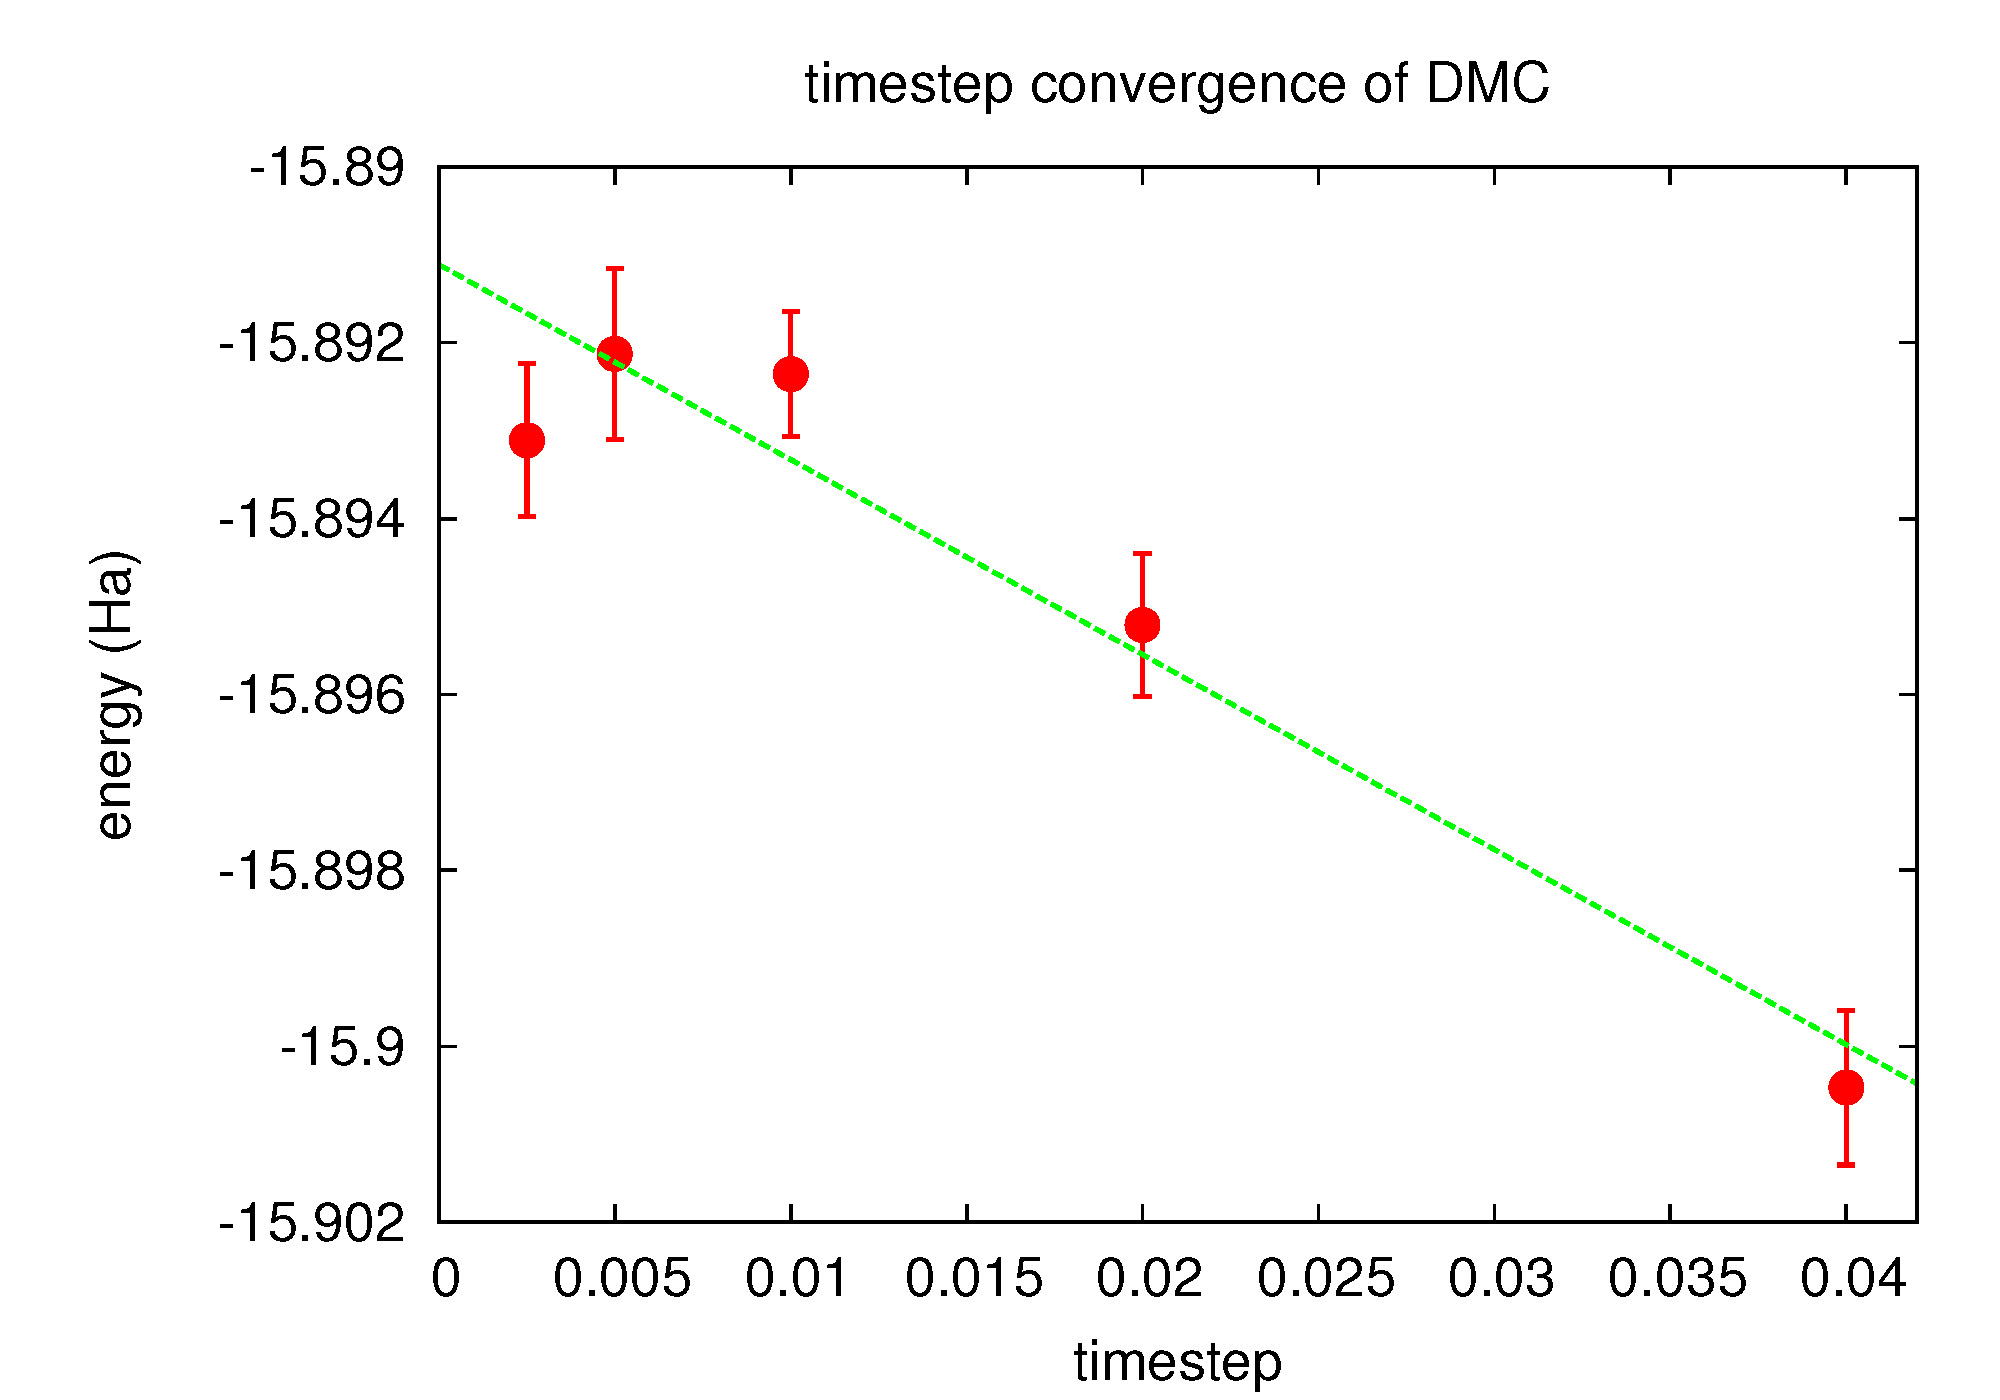
\includegraphics[trim = 0mm 0mm 0mm 0mm, clip,width=0.75\columnwidth]{./figures/lab_qmc_basics_timestep_conv.dmn}
\else
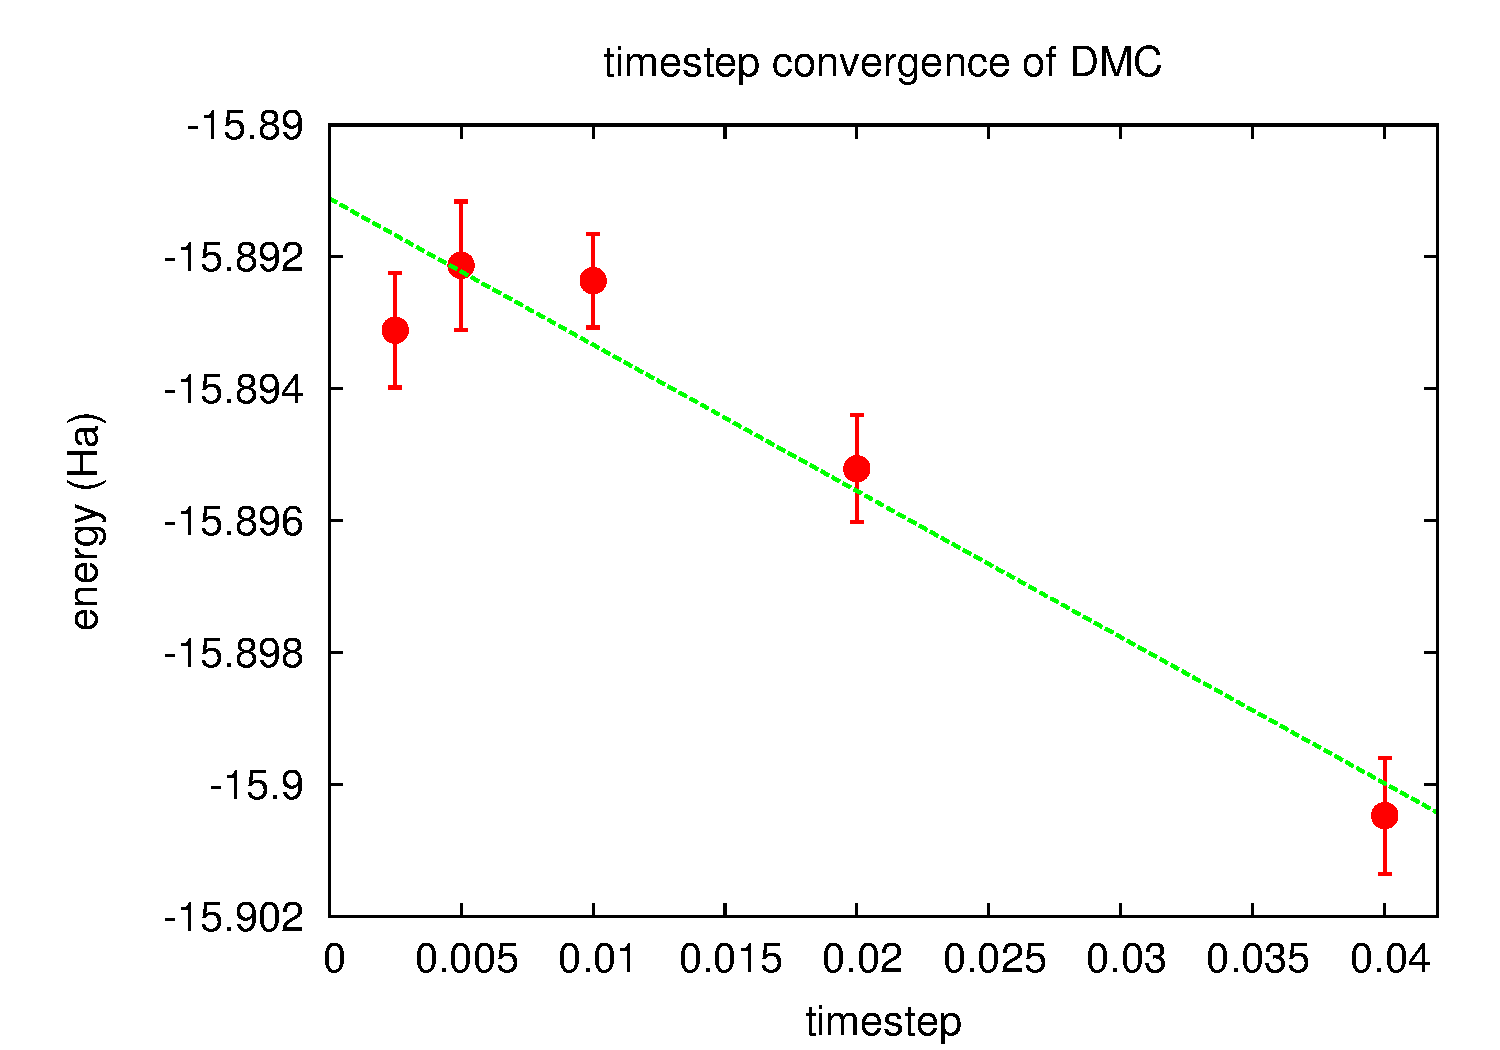
\includegraphics[trim = 0mm 0mm 0mm 0mm, clip,width=0.75\columnwidth]{./figures/lab_qmc_basics_timestep_conv.pdf}
\fi
\end{center}
\caption{Linear fit to DMC timestep data from \ishell{PlotTstepConv.pl}.}
\label{fig:timestep_conv}
\end{figure}


\vspace{1cm}
\begin{flushleft}
\textbf{\underline{Questions and Exercises}}
\end{flushleft}
\begin{enumerate}
  \item{What is the $\tau\rightarrow 0$ extrapolated value for the total energy?}
  \item{What is the maximum timestep you should use if you want to calculate the total energy to an accuracy of $0.05$ eV?  For convenience, $1~\textrm{Ha}=27.2113846~\textrm{eV}$.}
  \item{What is the acceptance ratio for this (bias$<0.05$ eV) run?  Does it follow the rule of thumb for sensible DMC (acceptance ratio $>99$\%) ?}
  \item{Check the fluctuations in the walker population (\ishell{qmca -t -q nw O.q0.dmc*dmc.dat --noac}).  Does the population seem to be stable?}
  \item{(Optional) Study population control bias for the oxygen atom.  Select a few population sizes \labsw{}{(use multiples of 512 to fit cleanly on a single Vesta partition)}.  Copy \ishell{O.q0.dmc.in.xml} to a new file and remove all but one DMC run (select a single timestep).  Make one copy of the new file for each population, set ``\ishell{samples}'', and choose a unique \ishell{id} in \ishell{<project/>}.  \labsw{}{Run one job at a time to avoid crowding the lab allocation.}  Use \ishell{qmca} to study the dependence of the DMC total energy on the walker population.  How large is the bias compared to timestep error?  What bias is incurred by following the ``rule of thumb'' of a couple thousand walkers?  Will population control bias generally be an issue for production runs on modern parallel machines?}
\end{enumerate}


\section{DMC timestep extrapolation II: O atom ionization potential}
In this section, we will repeat the calculations of the prior two sections (optimization, timestep extrapolation) for the $+1$ charge state of the oxygen atom.  Comparing the resulting 1st ionization potential (IP) with experimental data will complete our first test of the BFD oxygen pseudopotential.  In actual practice, higher IP's could also be tested prior to performing production runs.

Obtaining the timestep extrapolated DMC total energy for ionized oxygen should take much less (human) time than for the neutral case.  For convenience, the necessary steps are briefly summarized below.
\begin{enumerate}
  \item{Obtain DFT orbitals with Quantum ESPRESSO}
  \begin{enumerate}
    \item{Copy the DFT input (\ishell{O.q0.dft.in}) to \ishell{O.q1.dft.in}}
    \item{Edit \ishell{O.q1.dft.in} to match the +1 charge state of the oxygen atom}
    \begin{lstlisting}[style=espresso]
     ...
     prefix            = 'O.q1'
     ...
     tot_charge        = 1
     tot_magnetization = 3
     ...
    \end{lstlisting}
  \item{Perform the DFT run: \ifws\ishell{mpirun -np 4 pw.x -input O.q1.dft.in >&O.q1.dft.out&}
      \else\ishell{jobrun_vesta pw.x O.q1.dft.in}\fi}
  \end{enumerate}

  \item{Convert the orbitals to ESHDF format}
  \begin{enumerate}
    \item{Copy the pw2qmcpack input (\ishell{O.q0.p2q.in}) to \ishell{O.q1.p2q.in}}
    \item{Edit \ishell{O.q1.p2q.in} to match the file prefix used in DFT}
    \begin{verbatim}
     ...
     prefix = 'O.q1'
     ...
    \end{verbatim}
    \item{Perform the orbital conversion run: \ifws\ishell{mpirun -np 1 pw2qmcpack.x<O.q1.p2q.in>&O.q1.p2q.out&}\else\ishell{jobrun_vesta pw2qmcpack.x O.q1.p2q.in}\fi}
  \end{enumerate}

  \item{Optimize the Jastrow factor with QMCPACK}
  \begin{enumerate}
    \item{Copy the optimization input (\ishell{O.q0.opt.in.xml}) to \ishell{O.q1.opt.in.xml}}
    \item{Edit \ishell{O.q1.opt.in.xml} to match the file prefix used in DFT}
    \begin{lstlisting}[style=QMCPXML]
     ...
     <project id="O.q1.opt" series="0">
     ...
     <include href="O.q1.ptcl.xml"/>
     ...
     <include href="O.q1.wfs.xml"/>
     ...
    \end{lstlisting}
    \item{Edit the particle XML file (O.q1.ptcl.xml) to have open boundary conditions}
    \begin{lstlisting}[style=QMCPXML]
      <parameter name="bconds">
        n n n 
      </parameter>
    \end{lstlisting}
    \item{Add cutoffs to the Jastrow factors in the wavefunction XML file (O.q1.wfs.xml)}
    \begin{lstlisting}[style=QMCPXML]
      ...
      <correlation speciesA="u" speciesB="u" size="8" rcut="10.0">
      ...
      <correlation speciesA="u" speciesB="d" size="8" rcut="10.0">
      ...
      <correlation elementType="O" size="8" rcut="5.0">
      ...
    \end{lstlisting}
    \item{Perform the Jastrow optimization run: \ifws\ishell{mpirun -np 4 qmcpack O.q1.opt.in.xml >&O.q1.opt.out&}\else\ishell{jobrun_vesta qmcpack O.q1.opt.in.xml}\fi}
    \item{Identify the optimal set of parameters with \ishell{qmca} (\ishell{[your opt.xml]}).}
  \end{enumerate}

  \item{DMC timestep study with QMCPACK}
  \begin{enumerate}
    \item{Copy the DMC input (\ishell{O.q0.dmc.in.xml}) to \ishell{O.q1.dmc.in.xml}}
    \item{Edit \ishell{O.q1.dmc.in.xml} to use the DFT prefix and the optimal Jastrow}
    \begin{lstlisting}[style=QMCPXML]
     ...
     <project id="O.q1.dmc" series="0">
     ...
     <include href="O.q1.ptcl.xml"/>
     ...
     <include href="[your opt.xml]"/>
     ...
    \end{lstlisting}
    \item{Perform the DMC run: \ifws\ishell{mpirun -np 4 qmcpack O.q1.dmc.in.xml >&O.q1.dmc.out&}\else\ishell{jobrun_vesta qmcpack O.q1.dmc.in.xml}\fi}
    \item{Obtain the DMC total energy extrapolated to zero timestep with \ishell{PlotTstepConv.pl}.}
  \end{enumerate}
\end{enumerate}
The process listed above, which excludes additional steps for orbital generation and conversion, can become tedious to perform by hand in production settings where many calculations are often required.  For this reason automation tools are introduced for calculations involving the oxygen dimer in section \ref{sec:dimer_automation} of the lab.  

\vspace{1cm}
\begin{flushleft}
\textbf{\underline{Questions and Exercises}}
\end{flushleft}
\begin{enumerate}
  \item{What is the $\tau\rightarrow 0$ extrapolated DMC value for the 1st ionization potential of oxygen?}
  \item{How does the extrapolated value compare to the experimental IP?  Go to\newline \href{http://physics.nist.gov/PhysRefData/ASD/ionEnergy.html}{http://physics.nist.gov/PhysRefData/ASD/ionEnergy.html} and enter ``\ishell{O I}'' in the box labeled ``\ishell{Spectra}'' and click on the ``\ishell{Retrieve Data}'' button.  
%For comparison the LDA value is $12.25$ eV.
}
  \item{What can we conclude about the accuracy of the pseudopotential?  What factors complicate this assessment?}
  \item{Explore the sensitivity of the IP to the choice of timestep.  Type ``\ishell{./ip_conv.py}'' to view three timestep extrapolation plots: two for the $q=0,1$ total energies and one for the IP.  Is the IP more, less, or similarly sensitive to timestep than the total energy?}
  \item{What is the maximum timestep you should use if you want to calculate the ionization potential to an accuracy of $0.05$ eV?  What factor of cpu time is saved by assessing timestep convergence on the IP (a total energy difference) vs. a single total energy?}
  \item{Are the acceptance ratio and population fluctuations reasonable for the $q=1$ calculations?}
\end{enumerate}




\section{DMC workflow automation with Nexus}
Production QMC projects are often composed of many similar workflows.  The simplest of these is a single DMC calculation involving four different compute jobs:
\begin{enumerate}
  \item{Orbital generation via Quantum ESPRESSO or GAMESS.}
  \item{Conversion of orbital data via \ishell{pw2qmcpack.x} or \ishell{convert4qmc}.}
  \item{Optimization of Jastrow factors via QMCPACK.}
  \item{DMC calculation via QMCPACK.}
\end{enumerate}
Simulation workflows quickly become more complex with increasing costs in terms of human time for the researcher.  Automation tools can decrease both human time and error if used well.

The set of automation tools we will be using is known as Nexus \cite{Krogel2016nexus}, which is distributed with QMCPACK.  Nexus is capable of generating input files, submitting and monitoring compute jobs, passing data between simulations (such as relaxed structures, orbital files, optimized Jastrow parameters, etc.), and data analysis.  The user interface to Nexus is through a set of functions defined in the Python programming language.  User scripts that execute simple workflows resemble input files and do not require programming experience.  More complex workflows require only basic programming constructs (\emph{e.g.} for loops and if statements).  Nexus input files/scripts should be easier to navigate than QMCPACK input files and more efficient than submitting all the jobs by hand.

Nexus is driven by simple user-defined scripts that resemble keyword-driven input files.  An example Nexus input file that performs a single VMC calculation (with pre-generated orbitals) is shown below.  Take a moment to read it over and especially note the comments (prefixed with ``\ishell{\#}'') explaining most of the contents.  If the input syntax is unclear you may want to consult portions of appendix \ref{app:python_basics}, which gives a condensed summary of Python constructs.  An additional example and details about the inner workings of Nexus can be found in the reference publication \cite{Krogel2016nexus}. 

%For more information about the functionality and effective use of Nexus, consult \ishell{docs/Nexus.pdf}.  

%More information can be found in the user guide distributed with QMCPACK, although examples in this lab series and \ishell{Nexus.pdf} are more up to date (if \ishell{qmcpack} is the location of your QMCPACK distribution, the user guide can be found at \ishell{qmcpack/nexus/documentation/nexus\_user\_guide.pdf}).

\ifws
\begin{lstlisting}[style=Python]
#! /usr/bin/env python

# import Nexus functions
from nexus import settings,job,get_machine,run_project 
from nexus import generate_physical_system
from nexus import generate_qmcpack,vmc

settings(                             # Nexus settings
    pseudo_dir    = './pseudopotentials', # location of PP files
    runs          = '',                   # root directory for simulations
    results       = '',                   # root directory for simulation results
    status_only   = 0,                    # show simulation status, then exit
    generate_only = 0,                    # generate input files, then exit
    sleep         = 3,                    # seconds between checks on sim. progress
    machine       = 'ws4',                # workstation with 4 cores
    ) 

qmcjob = job(                         # specify job parameters
    cores   = 4,                          # use 4 MPI tasks
    threads = 1,                          # 1 OpenMP thread per node
    app     = 'qmcpack'                   # use QMCPACK executable (assumed in PATH)
    )

qmc_calcs = [                         # list QMC calculation methods
    vmc(                                  #   VMC
        walkers     =   1,                #     1 walker
        warmupsteps =  50,                #    50 MC steps for warmup
        blocks      = 200,                #   200 blocks
        steps       =  10,                #    10 steps per block
        timestep    =  .4                 #   0.4 1/Ha timestep
        )]

dimer = generate_physical_system(     # make a dimer system
    type       = 'dimer',                 # system type is dimer
    dimer      = ('O','O'),               # dimer is two oxygen atoms
    separation = 1.2074,                  # separated by 1.2074 Angstrom
    Lbox       = 15.0,                    # simulation box is 15 Angstrom 
    units      = 'A',                     # Angstrom is dist. unit
    net_spin   = 2,                       # nup-ndown is 2
    O          = 6                        # pseudo-oxygen has 6 valence el.
    )

qmc = generate_qmcpack(                # make a qmcpack simulation 
    identifier   = 'example',             # prefix files with 'example'
    path         = 'scale_1.0',           # run in ./scale_1.0 directory
    system       = dimer,                 # run the dimer system
    job          = qmcjob,                # set job parameters
    input_type   = 'basic',               # basic qmcpack inputs given below    
    pseudos      = ['O.BFD.xml'],         # list of PP's to use
    orbitals_h5  = 'O2.pwscf.h5',         # file with orbitals from DFT
    bconds       = 'nnn',                 # open boundary conditions
    jastrows     = [],                    # no jastrow factors
    calculations = qmc_calcs              # QMC calculations to perform
    )
                       
run_project(qmc)                       # write input file and submit job
\end{lstlisting}

\else

\begin{lstlisting}[style=Python]
#! /usr/bin/env python

# import Nexus functions
from nexus import settings,job,get_machine,run_project 
from nexus import generate_physical_system
from nexus import generate_qmcpack,vmc

settings(                             # Nexus settings
    pseudo_dir    = './pseudopotentials', # location of PP files
    runs          = '',                   # root directory for simulations
    results       = '',                   # root directory for simulation results
    status_only   = 0,                    # show simulation status, then exit
    generate_only = 0,                    # generate input files, then exit
    sleep         = 3,                    # seconds between checks on sim. progress
    machine       = 'vesta',              # name of local machine
    account       = 'QMCPACK-Training'    # charge account for cpu time
    ) 

vesta = get_machine('vesta')          # allow max of one job at a time (lab only)
vesta.queue_size = 1

qmcjob = job(                         # specify job parameters
    nodes   = 32,                         # use 32 Vesta nodes
    threads = 16,                         # 16 OpenMP threads per node (32 MPI tasks)
    hours   = 1,                          # wallclock limit of 1 hour
                                          # use QMCPACK executable
    app     = '/soft/applications/qmcpack/Binaries/qmcpack'
    )

qmc_calcs = [                         # list QMC calculation methods
    vmc(                                  #   VMC
        walkers     =   1,                #     1 walker
        warmupsteps =  50,                #    50 MC steps for warmup
        blocks      = 200,                #   200 blocks
        steps       =  10,                #    10 steps per block
        timestep    =  .4                 #   0.4 1/Ha timestep
        )]

dimer = generate_physical_system(     # make a dimer system
    type       = 'dimer',                 # system type is dimer
    dimer      = ('O','O'),               # dimer is two oxygen atoms
    separation = 1.2074,                  # separated by 1.2074 Angstrom
    Lbox       = 15.0,                    # simulation box is 15 Angstrom 
    units      = 'A',                     # Angstrom is dist. unit
    net_spin   = 2,                       # nup-ndown is 2
    O          = 6                        # pseudo-oxygen has 6 valence el.
    )

qmc = generate_qmcpack(                # make a qmcpack simulation 
    identifier   = 'example',             # prefix files with 'example'
    path         = 'scale_1.0',           # run in ./scale_1.0 directory
    system       = dimer,                 # run the dimer system
    job          = qmcjob,                # set job parameters
    input_type   = 'basic',               # basic qmcpack inputs given below    
    pseudos      = ['O.BFD.xml'],         # list of PP's to use
    orbitals_h5  = 'O2.pwscf.h5',         # file with orbitals from DFT
    bconds       = 'nnn',                 # open boundary conditions
    jastrows     = [],                    # no jastrow factors
    calculations = qmc_calcs              # QMC calculations to perform
    )
                       
run_project(qmc)                       # write input file and submit job
\end{lstlisting}
\fi





\section{Automated binding curve of the oxygen dimer}
\label{sec:dimer_automation}
In this section we will use Nexus to calculate the DMC total energy of the oxygen dimer over a series of bond lengths.  The equilibrium bond length and binding energy of the dimer will be determined by performing a polynomial fit to the data (Morse potential fits should be preferred in production tests).  Comparing these values with corresponding experimental data provides a second test of the BFD pseudopotential for oxygen.

Enter the \ishell{oxygen\_dimer} directory.  Copy your BFD pseudopotential from the atom runs into \ishell{oxygen\_dimer/pseudopotentials} (be sure to move both files: \ishell{.upf} and \ishell{.xml}).  Open \ishell{O\_dimer.py} with a text editor.  The overall format is similar to the example file shown in the last section.  
%The header material, including Nexus imports, settings, and the job parameters for QMC are identical.  
The main difference is that a full workflow of runs (DFT orbital generation, orbital conversion, optimization and DMC) are being performed rather than a single VMC run.  


%Following the job parameters, inputs for the optimization method are given.  The keywords should all be familiar from the QMCPACK XML input files you used previously:
%\begin{lstlisting}
%linopt1 = linear(
%    energy               = 0.0,
%    unreweightedvariance = 1.0,
%    reweightedvariance   = 0.0,
%    timestep             = 0.4,
%    samples              = 10240, 
%    warmupsteps          = 50,
%    blocks               = 200,
%    substeps             = 1,
%    nonlocalpp           = True,
%    usebuffer            = True,
%    walkers              = 1,
%    minwalkers           = 0.5,
%    maxweight            = 1e9,
%    usedrift             = True,
%    minmethod            = 'quartic',
%    beta                 = 0.025,
%    exp0                 = -16,
%    bigchange            = 15.0,
%    alloweddifference    = 1e-4,
%    stepsize             = 0.2,
%    stabilizerscale      = 1.0,
%    nstabilizers         = 3
%    )
%\end{lstlisting}
%
%%\hide{
%\noindent
%Requesting multiple loop's with different numbers of samples is more compact than in XML:
%\begin{lstlisting}
%linopt1 = ...
%
%linopt2 = linopt1.copy()  
%linopt2.samples = 61440 # opt w/ 61440 samples
%
%opt_calcs = [loop(max=4,qmc=linopt1), # loops over opt's
%             loop(max=8,qmc=linopt2)]
%\end{lstlisting}
%%}
%
%\noindent
%The VMC/DMC method inputs should also look familiar:
%\begin{lstlisting}
%qmc_calcs = [
%    vmc(
%        walkers     =   1,
%        warmupsteps =  30,
%        blocks      =  20,
%        steps       =  10,
%        substeps    =   2,
%        timestep    =  .4,
%        samples     = 2048
%        ),
%    dmc(
%        warmupsteps   = 100, 
%        blocks        = 400,
%        steps         =  32,
%        timestep      = 0.01,
%        nonlocalmoves = True
%        )
%    ]
%\end{lstlisting}


As in the example in the last section, the oxygen dimer is generated with the \ishell{generate\_physical\_system} function:
\begin{lstlisting}[style=Python]
dimer = generate_physical_system(
    type       = 'dimer',
    dimer      = ('O','O'),
    separation = 1.2074*scale,
    Lbox       = 10.0,
    units      = 'A',
    net_spin   = 2,
    O          = 6
    )
\end{lstlisting}
\noindent
Similar syntax can be used to generate crystal structures or to specify systems with arbitrary atomic configurations and simulation cells.  Notice that a ``\ishell{scale}'' variable has been introduced to stretch or compress the dimer.  

Next, objects representing a Quantum ESPRESSO (PWSCF) run and subsequent orbital conversion step are constructed with respective \ishell{generate\_*} functions:
\begin{lstlisting}[style=Python]
dft = generate_pwscf(
    identifier   = 'dft',
    ...
    input_dft    = 'lda',
    ...
    )
sims.append(dft)

# describe orbital conversion run                                                                    
p2q = generate_pw2qmcpack(
    identifier   = 'p2q',
    ...
    dependencies = (dft,'orbitals'),
    )
sims.append(p2q)
\end{lstlisting}
Note the \ishell{dependencies} keyword.  This keyword is used to construct workflows out of otherwise separate runs.  In this case, the dependency indicates that the orbital conversion run must wait for the DFT to finish prior to starting.

Objects representing QMCPACK simulations are then constructed with the \ishell{generate\_qmcpack} function:
\begin{lstlisting}[style=Python]
opt = generate_qmcpack(
    identifier   = 'opt',
    ...
    jastrows     = [('J1','bspline',8,5.0), 
                    ('J2','bspline',8,10.0)],
    calculations = [
        loop(max=12,
             qmc=linear(
                energy               = 0.0,
                unreweightedvariance = 1.0,
                reweightedvariance   = 0.0,
                timestep             = 0.3,
                samples              = 61440,
                warmupsteps          = 50,
                blocks               = 200,
                substeps             = 1,
                nonlocalpp           = True,
                usebuffer            = True,
                walkers              = 1,
                minwalkers           = 0.5,
                maxweight            = 1e9,
                usedrift             = False,
                minmethod            = 'quartic',
                beta                 = 0.025,
                exp0                 = -16,
                bigchange            = 15.0,
                alloweddifference    = 1e-4,
                stepsize             = 0.2,
                stabilizerscale      = 1.0,
                nstabilizers         = 3,
                )
             )
        ],
    dependencies = (p2q,'orbitals'),
    )
sims.append(opt)

qmc = generate_qmcpack(
    identifier   = 'qmc',
    ...
    jastrows     = [],            
    calculations = [
        vmc(
            walkers     =   1,
            warmupsteps =  30,
            blocks      =  20,
            steps       =  10,
            substeps    =   2,
            timestep    =  .4,
            samples     = 2048
            ),
        dmc(
            warmupsteps   = 100,
            blocks        = 400,
            steps         =  32,
            timestep      = 0.01,
            nonlocalmoves = True,
            )
        ],
    dependencies = [(p2q,'orbitals'),(opt,'jastrow')],
    )
sims.append(qmc)
\end{lstlisting}
\noindent
Shared details such as the run directory, job, pseudopotentials, and orbital file have been omitted (\ishell{...}).  The ``\ishell{opt}'' run will optimize a 1-body B-spline Jastrow with 8 knots having a cutoff of 5.0 Bohr and a B-spline Jastrow (for up-up and up-down correlations) with 8 knots and cutoffs of 10.0 Bohr.  The Jastrow list for the DMC run is empty and the usage of \ishell{dependencies} above indicates that the DMC run depends on the optimization run for the Jastrow factor.  Nexus will submit the ``\ishell{opt}'' run first and upon completion it will scan the output, select the optimal set of parameters, pass the Jastrow information to the ``\ishell{qmc}'' run and then submit the DMC job.  Independent job workflows are submitted in parallel when permitted \labsw{}{(we have explicitly limited this for this lab by setting \ishell{queue\_size=2} for Vesta)}.  No input files are written or job submissions made until the ``\ishell{run\_project}'' function is reached:
\begin{lstlisting}[style=Python]
run_project(sims)
\end{lstlisting}
\noindent
All of the simulations objects have been collected into a list (\ishell{sims}) for submission.

As written, \ishell{O\_dimer.py} will only perform calculations at the equilibrium separation distance of 1.2074 Angstrom, since the list of scaling factors (representing stretching or compressing the dimer) only contains one value (\ishell{scales = [1.00]}).  Modify the file now to perform DMC calculations across a range of separation distances with each DMC run using the Jastrow factor optimized at the equilibrium separation distance.  Specifically, you will want to change the list of scaling factors to include both compression (\ishell{scale<1.0}) and stretch (\ishell{scale>1.0}): 
\begin{lstlisting}[style=Python]
scales = [1.00,0.90,0.95,1.05,1.10]
\end{lstlisting}
\noindent
Note that ``\ishell{1.00}'' is left in front because we are going to optimize the Jastrow factor first at the equilibrium separation and reuse this Jastrow factor for all other separation distances.  This procedure is used because it can reduce variations in localization errors (due to pseudopotentials in DMC) along the binding curve. 

Change the ``\ishell{status\_only}'' parameter in the ``\ishell{settings}'' function to \ishell{1} and type ``./O\_dimer.py'' at the command line.  This will print the status of all simulations:
\begin{shade}
Project starting 
  checking for file collisions 
  loading cascade images 
    cascade 0 checking in 
    cascade 10 checking in 
    cascade 4 checking in 
    cascade 13 checking in 
    cascade 7 checking in 
  checking cascade dependencies 
    all simulation dependencies satisfied 
  
  cascade status 
    setup, sent_files, submitted, finished, got_output, analyzed 
    000000  dft     ./scale_1.0 
    000000  p2q     ./scale_1.0 
    000000  opt     ./scale_1.0 
    000000  qmc     ./scale_1.0 
    000000  dft     ./scale_0.9 
    000000  p2q     ./scale_0.9 
    000000  qmc     ./scale_0.9 
    000000  dft     ./scale_0.95 
    000000  p2q     ./scale_0.95 
    000000  qmc     ./scale_0.95 
    000000  dft     ./scale_1.05 
    000000  p2q     ./scale_1.05 
    000000  qmc     ./scale_1.05 
    000000  dft     ./scale_1.1 
    000000  p2q     ./scale_1.1 
    000000  qmc     ./scale_1.1 
    setup, sent_files, submitted, finished, got_output, analyzed 
\end{shade}
\noindent
In this case, five simulation ``cascades'' (workflows) have been identified, each one starting and ending with ``\ishell{dft}'' and ``\ishell{qmc}'' runs, respectively.  The six status flags (\ishell{setup}, \ishell{sent\_files}, \ishell{submitted}, \ishell{finished}, \ishell{got\_output}, \ishell{analyzed}) each show \ishell{0}, indicating that no work has been done yet.  

Now change ``\ishell{status\_only}'' back to \ishell{0}, set ``\ishell{generate\_only}'' to \ishell{1}, and run \ishell{O\_dimer.py} again.  This will perform a dry-run of all simulations.  The dry-run should finish in about 20 seconds:
\ifws
\begin{shade}
Project starting 
  checking for file collisions 
  loading cascade images 
    cascade 0 checking in 
    cascade 10 checking in 
    cascade 4 checking in 
    cascade 13 checking in 
    cascade 7 checking in 
  checking cascade dependencies 
    all simulation dependencies satisfied 
  
  starting runs:
  ~~~~~~~~~~~~~~~~~~~~~~~~~~~~~~ 
  poll 0  memory 91.03 MB 
    Entering ./scale_1.0 0 
      writing input files  0 dft 
    Entering ./scale_1.0 0 
      sending required files  0 dft 
      submitting job  0 dft 
  ...
  poll 1  memory 91.10 MB 
  ...
    Entering ./scale_1.0 0 
      Would have executed:  
        export OMP_NUM_THREADS=1
        mpirun -np 4 pw.x -input dft.in 

  poll 2  memory 91.10 MB 
    Entering ./scale_1.0 0 
      copying results  0 dft 
    Entering ./scale_1.0 0 
      analyzing  0 dft 
  ...
  poll 3  memory 91.10 MB 
    Entering ./scale_1.0 1 
      writing input files  1 p2q 
    Entering ./scale_1.0 1 
      sending required files  1 p2q 
      submitting job  1 p2q 
  ...
    Entering ./scale_1.0 1 
      Would have executed:  
        export OMP_NUM_THREADS=1
        mpirun -np 1 pw2qmcpack.x<p2q.in 

  poll 4  memory 91.10 MB 
    Entering ./scale_1.0 1 
      copying results  1 p2q 
    Entering ./scale_1.0 1 
      analyzing  1 p2q 
  ...
  poll 5  memory 91.10 MB 
    Entering ./scale_1.0 2 
      writing input files  2 opt 
    Entering ./scale_1.0 2 
      sending required files  2 opt 
      submitting job  2 opt 
  ...
    Entering ./scale_1.0 2 
      Would have executed:  
        export OMP_NUM_THREADS=1
        mpirun -np 4 qmcpack opt.in.xml 

  poll 6  memory 91.16 MB 
    Entering ./scale_1.0 2 
      copying results  2 opt 
    Entering ./scale_1.0 2 
      analyzing  2 opt 
  ...
  poll 7  memory 93.00 MB 
    Entering ./scale_1.0 3 
      writing input files  3 qmc 
    Entering ./scale_1.0 3 
      sending required files  3 qmc 
      submitting job  3 qmc 
  ...
    Entering ./scale_1.0 3 
      Would have executed:  
        export OMP_NUM_THREADS=1
        mpirun -np 4 qmcpack qmc.in.xml 
  ...
  poll 17  memory 93.06 MB 
Project finished
\end{shade}
\else
\begin{shade}
Project starting 
  checking for file collisions 
  loading cascade images 
    cascade 0 checking in 
    cascade 10 checking in 
    cascade 4 checking in 
    cascade 13 checking in 
    cascade 7 checking in 
  checking cascade dependencies 
    all simulation dependencies satisfied 
  
  starting runs:
  ~~~~~~~~~~~~~~~~~~~~~~~~~~~~~~ 
  poll 0  memory 91.03 MB 
    Entering ./scale_1.0 0 
      writing input files  0 dft 
    Entering ./scale_1.0 0 
      sending required files  0 dft 
      submitting job  0 dft 
  ...
  poll 1  memory 91.10 MB 
  ...
    Entering ./scale_1.0 1 
      Would have executed:  qsub --mode script --env BG_SHAREDMEMSIZE=32 dft.qsub.in 

  poll 2  memory 91.10 MB 
    Entering ./scale_1.0 0 
      copying results  0 dft 
    Entering ./scale_1.0 0 
      analyzing  0 dft 
  ...
  poll 3  memory 91.10 MB 
    Entering ./scale_1.0 1 
      writing input files  1 p2q 
    Entering ./scale_1.0 1 
      sending required files  1 p2q 
      submitting job  1 p2q 
  ...
    Entering ./scale_1.0 2 
      Would have executed:  qsub --mode script --env BG_SHAREDMEMSIZE=32 p2q.qsub.in 

  poll 4  memory 91.10 MB 
    Entering ./scale_1.0 1 
      copying results  1 p2q 
    Entering ./scale_1.0 1 
      analyzing  1 p2q
  ... 

  poll 5  memory 91.10 MB 
    Entering ./scale_1.0 2 
      writing input files  2 opt 
    Entering ./scale_1.0 2 
      sending required files  2 opt 
      submitting job  2 opt 
  ...
    Entering ./scale_1.0 3 
      Would have executed:  qsub --mode script --env BG_SHAREDMEMSIZE=32 opt.qsub.in 

  poll 6  memory 91.16 MB 
    Entering ./scale_1.0 2 
      copying results  2 opt 
    Entering ./scale_1.0 2 
      analyzing  2 opt 
  ...
  poll 7  memory 93.00 MB 
    Entering ./scale_1.0 3 
      writing input files  3 qmc 
    Entering ./scale_1.0 3 
      sending required files  3 qmc 
      submitting job  3 qmc 
  ...
    Entering ./scale_1.0 4 
      Would have executed:  qsub --mode script --env BG_SHAREDMEMSIZE=32 qmc.qsub.in 
  ...

  poll 17  memory 93.00 MB 
Project finished
\end{shade}
\fi

\noindent
Nexus polls the simulation status every 3 seconds and sleeps in between.  The ``scale\_*'' directories should now contain several files:
\ifws
\begin{shade}
scale_1.0
   dft.in
   O.BFD.upf
   O.BFD.xml
   opt.in.xml
   p2q.in
   pwscf_output
   qmc.in.xml
   sim_dft/
       analyzer.p
       input.p
       sim.p
   sim_opt/
       analyzer.p
       input.p
       sim.p
   sim_p2q/
       analyzer.p
       input.p
       sim.p
   sim_qmc/
       analyzer.p
       input.p
       sim.p
\end{shade}
\else
\begin{shade}
scale_1.0
   dft.in
   dft.qsub.in
   O.BFD.upf
   O.BFD.xml
   opt.in.xml
   opt.qsub.in
   p2q.in
   p2q.qsub.in
   pwscf_output
   qmc.in.xml
   qmc.qsub.in
   sim_dft/
       analyzer.p
       input.p
       sim.p
   sim_opt/
       analyzer.p
       input.p
       sim.p
   sim_p2q/
       analyzer.p
       input.p
       sim.p
   sim_qmc/
       analyzer.p
       input.p
       sim.p
\end{shade}
\fi
\noindent
Take a minute to inspect the generated input (\ishell{dft.in}, \ishell{p2q.in}, \ishell{opt.in.xml}, \ishell{qmc.in.xml}) \labsw{}{and submission (\ishell{dft.qsub.in}, \ishell{p2q.qsub.in}, \ishell{opt.qsub.in}, \ishell{qmc.qsub.in})} files.  The pseudopotential files (\ishell{O.BFD.upf} and \ishell{O.BFD.xml}) have been copied into each local directory. Four additional directories have been created: \ishell{sim\_dft},  \ishell{sim\_p2q}, \ishell{sim\_opt} and \ishell{sim\_qmc}.  The \ishell{sim.p} files in each directory contain the current status of each simulation.  If you run \ishell{O\_dimer.py} again, it should not attempt to rerun any of the simulations:   
\begin{shade}
Project starting 
  checking for file collisions 
  loading cascade images 
    cascade 0 checking in 
    cascade 10 checking in 
    cascade 4 checking in 
    cascade 13 checking in 
    cascade 7 checking in 
  checking cascade dependencies 
    all simulation dependencies satisfied 
  
  starting runs:
  ~~~~~~~~~~~~~~~~~~~~~~~~~~~~~~ 
  poll 0  memory 64.25 MB 
Project finished
\end{shade}
\noindent
This way one can continue to add to the \ishell{O\_dimer.py} file (\emph{e.g.} adding more separation distances) without worrying about duplicate job submissions.

Let's actually submit the jobs in the dimer workflow now.  Reset the state of the simulations by removing the \ishell{sim.p} files (``\ishell{rm ./scale*/sim*/sim.p}''), set ``\ishell{generate\_only}'' to \ishell{0}, and rerun \ishell{O\_dimer.py}.  It should take about 20 minutes for all the jobs to complete.  You may wish to open another terminal to monitor the progress of the individual jobs while the current terminal runs \ishell{O\_dimer.py} in the foreground.  You can begin the first exercise below once the optimization job completes.

\vspace{3cm}
\begin{flushleft}
\textbf{\underline{Questions and Exercises}}
\end{flushleft}
\begin{enumerate}
  \item{Evaluate the quality of the optimization at \ishell{scale=1.0} using the \ishell{qmca} tool.  Did the optimization succeed?  How does the variance compare with the neutral oxygen atom?  Is the wavefunction of similar quality to the atomic case?}

  \item{Evaluate the traces of the local energy and the DMC walker population for each separation distance with the \ishell{qmca} tool.  Are there any anomalies in the runs?  Is the acceptance ratio reasonable?  Is the wavefunction of similar quality across all separation distances?}

  \item{Use the \ishell{dimer\_fit.py} tool located in \ishell{oxygen\_dimer} to fit the oxygen dimer binding curve.   To get the binding energy of the dimer, we will need the DMC energy of the atom.  Before performing the fit, answer: What DMC timestep should be used for the oxygen atom results?  The tool accepts three arguments (``\ishell{./dimer_fit.py P N E Eerr}''}), \ishell{P} is the prefix of the DMC input files (should be ``\ishell{qmc}'' at this point), \ishell{N} is the order of the fit (use 2 to start), \ishell{E} and \ishell{Eerr} are your DMC total energy and error bar, respectively for the oxygen atom (in eV).  A plot of the dimer data will be displayed and text output will show the DMC equilibrium bond length and binding energy as well as experimental values.  How accurately does your fit to the DMC data reproduce the experimental values?  What factors affect the accuracy of your results? 

  \item{Refit your data with a fourth-order polynomial.  How do your predictions change with a fourth-order fit?  Is a fourth-order fit appropriate for the available data?}
 
  \item{Add new ``\ishell{scale}'' values to the list in \ishell{O\_dimer.py} that interpolate between the original set (e.g. expand to \ishell{[1.00,0.90,0.925,0.95,0.975,1.025,1.05,1.075,1.10]}).  Perform the DMC calculations and redo the fits.  How accurately does your fit to the DMC data reproduce the experimental values?  Should this pseudopotential be used in production calculations?}

  \item{(Optional) Perform optimization runs at the extremal separation distances corresponding to \ishell{scale=[0.90,1.10]}}.  Are the individually optimized wavefunctions of significantly better quality than the one imported from \ishell{scale=1.00}?  Why?  What form of Jastrow factor might give an even better improvement? 
\end{enumerate}




\section{(Optional) Running your system with QMCPACK}\label{sec:your_system}
This section covers a fairly simple route to get started on QMC calculations of an arbitrary system of interest using the Nexus workflow management system to setup input files and optionally perform the runs.  The example provided in this section uses QM Espresso (PWSCF) to generate the orbitals forming the Slater determinant part of the trial wavefunction.  PWSCF is a natural choice for solid state systems and it can be used for surface/slab and molecular systems as well, albeit at the price of describing additional vacuum space with plane waves.

To start out with, you will need pseudopotentials (PP's) for each element in your system in both the UPF (PWSCF) and FSATOM/XML (QMCPACK) formats.  A good place to start is the Burkatzki-Filippi-Dolg (BFD) pseudopotential database \newline (\href{http://www.burkatzki.com/pseudos/index.2.html}{http://www.burkatzki.com/pseudos/index.2.html}), which we have already used in our study of the oxygen atom.  The database does not contain PP's for the 4th and 5th row transition metals or any of the lanthanides or actinides.  If you need a PP that is not in the BFD database, you may need to generate and test one manually (\emph{e.g.} with OPIUM, \href{http://opium.sourceforge.net/}{http://opium.sourceforge.net/}).  Otherwise, use \ishell{ppconvert} as outlined in section \ref{sec:lqb_pseudo} to obtain PP's in the formats used by PWSCF and QMCPACK.  Enter the \ishell{your\_system} lab directory and place the converted PP's in \ishell{your\_system/pseudopotentials}.

Before performing production calculations (more than just the initial setup in this section) be sure to converge the plane wave energy cutoff in PWSCF as these PP's can be rather hard, sometimes requiring cutoffs in excess of 300 Ry.  Depending on the system under study, the amount of memory required to represent the orbitals (QMCPACK uses 3D B-splines) becomes prohibitive and one may be forced to search for softer PP's.

Beyond pseudopotentials, all that is required to get started are the atomic positions and the dimensions/shape of the simulation cell.  The Nexus file \ishell{example.py} illustrates how to setup PWSCF and QMCPACK input files by providing minimal information regarding the physical system (an 8-atom cubic cell of diamond in the example).  Most of the contents should be familiar from your experience with the automated calculations of the oxygen dimer binding curve in section \ref{sec:dimer_automation} (if you've skipped ahead you may want to skim that section for relevant information).  The most important change is the expanded description of the physical system:

\begin{lstlisting}[style=Python]
# details of your physical system (diamond conventional cell below)
my_project_name = 'diamond_vmc'   # directory to perform runs
my_dft_pps      = ['C.BFD.upf']   # pwscf pseudopotentials
my_qmc_pps      = ['C.BFD.xml']   # qmcpack pseudopotentials

#  generate your system
#    units      :  'A'/'B' for Angstrom/Bohr
#    axes       :  simulation cell axes in cartesian coordinates (a1,a2,a3)
#    elem       :  list of atoms in the system
#    pos        :  corresponding atomic positions in cartesian coordinates
#    kgrid      :  Monkhorst-Pack grid
#    kshift     :  Monkhorst-Pack shift (between 0 and 0.5)
#    net_charge :  system charge in units of e
#    net_spin   :  # of up spins - # of down spins
#    C = 4      :  (pseudo) carbon has 4 valence electrons
my_system = generate_physical_system(
    units      = 'A',
    axes       = [[ 3.57000000e+00, 0.00000000e+00, 0.00000000e+00],
                  [ 0.00000000e+00, 3.57000000e+00, 0.00000000e+00],
                  [ 0.00000000e+00, 0.00000000e+00, 3.57000000e+00]],
    elem       = ['C','C','C','C','C','C','C','C'],
    pos        = [[ 0.00000000e+00, 0.00000000e+00, 0.00000000e+00],
                  [ 8.92500000e-01, 8.92500000e-01, 8.92500000e-01],
                  [ 0.00000000e+00, 1.78500000e+00, 1.78500000e+00],
                  [ 8.92500000e-01, 2.67750000e+00, 2.67750000e+00],
                  [ 1.78500000e+00, 0.00000000e+00, 1.78500000e+00],
                  [ 2.67750000e+00, 8.92500000e-01, 2.67750000e+00],
                  [ 1.78500000e+00, 1.78500000e+00, 0.00000000e+00],
                  [ 2.67750000e+00, 2.67750000e+00, 8.92500000e-01]],
    kgrid      = (1,1,1),
    kshift     = (0,0,0),
    net_charge = 0,
    net_spin   = 0,
    C          = 4       # one line like this for each atomic species
    )

my_bconds       = 'ppp'  #  ppp/nnn for periodic/open BC's in QMC
                         #  if nnn, center atoms about (a1+a2+a3)/2
\end{lstlisting}

If you have a system you would like to try with QMC, make a copy of \ishell{example.py} and fill in the relevant information about the pseudopotentials, simulation cell axes, and atomic species/positions.  Otherwise, you can proceed with \ishell{example.py} as it is.

%The other new aspects are two additional compute jobs to generate the orbitals with PWSCF and convert them into the ESHDF format with \ishell{pw2qmcpack.x}:

%\begin{lstlisting}[style=Python]
%# scf run to generate orbitals
%scf = generate_pwscf(
%    identifier   = 'scf',
%    path         = my_project_name,
%    job          = Job(nodes=32,hours=2,app=pwscf),
%    input_type   = 'scf',
%    system       = my_system,
%    pseudos      = my_dft_pps,
%    input_dft    = 'lda', 
%    ecut         = 200,   # PW energy cutoff in Ry
%    conv_thr     = 1e-8, 
%    mixing_beta  = .7,
%    nosym        = True,
%    wf_collect   = True
%    )
%
%# conversion step to create h5 file with orbitals
%p2q = generate_pw2qmcpack(
%    identifier   = 'p2q',
%    path         = my_project_name,
%    job          = Job(cores=1,hours=2,app=pw2qmcpack),
%    write_psir   = False,
%    dependencies = (scf,'orbitals')
%    )
%\end{lstlisting}

Set ``\ishell{generate\_only}'' to \ishell{1} and type ``\ishell{./example.py}'' or similar to generate the input files.  All files will be written to ``\ishell{./diamond\_vmc}'' (``\ishell{./[my\_project\_name]}'' if you have changed ``\ishell{my\_project\_name}'' in the file).  The input files for PWSCF, pw2qmcpack, and QMCPACK are \ishell{scf.in}, \ishell{pw2qmcpack.in}, and \ishell{vmc.in.xml}, respectively.  Take some time to inspect the generated input files.  If you have questions about the file contents, or run into issues with the generation process, feel free to consult with a lab instructor.  

If desired, you can submit the runs directly with \ishell{example.py}.  To do this, first reset the Nexus simulation record by typing ``\ishell{rm ./diamond\_vmc/sim*/sim.p}'' or similar and set ``\ishell{generate\_only}'' back to \ishell{0}.  Next rerun \ishell{example.py}  (you may want to redirect the text output).  

Alternatively the runs can be submitted by hand:
\ifws
\begin{shade}
mpirun -np 4 pw.x<scf.in>&scf.out&

(wait until JOB DONE appears in scf.out)

mpirun -np 1 pw2qmcpack.x<p2q.in>&p2q.out&
\end{shade}
\else
\begin{shade}
qsub --mode script --env BG_SHAREDMEMSIZE=32 scf.qsub.in

(wait until JOB DONE appears in scf.output)

qsub --mode script --env BG_SHAREDMEMSIZE=32 p2q.qsub.in
\end{shade}
\fi
Once the conversion process has finished the orbitals should be located in the file \newline \ishell{diamond\_vmc/pwscf\_output/pwscf.pwscf.h5}.  Open \ishell{diamond\_vmc/vmc.in.xml} and replace ``\ishell{MISSING.h5}'' with ``\ishell{./pwscf\_output/pwscf.pwscf.h5}''.  Next submit the VMC run:
\ifws
\begin{shade}
mpirun -np 4 qmcpack vmc.in.xml>&vmc.out&
\end{shade}
\else
\begin{shade}
qsub --mode script --env BG_SHAREDMEMSIZE=32 vmc.qsub.in
\end{shade}
\fi
Note: If your system is large, the above process may not complete within the time frame of this lab.  Working with a stripped down (but relevant) example is a good idea for exploratory runs.

Once the runs have finished, you may want to begin exploring Jastrow optimization and DMC for your system.  Example calculations are provided at the end of \ishell{example.py} in the commented out text.



%\section{(Optional) Revisiting the oxygen atom: 3-body Jastrow \& population control bias}

%\subsection{Optimization of 3-body Jastrow factors}

%\subsection{Investigation of DMC population control bias}




% cover basic python elsewhere in the manual?  refer to Nexus user guide or websites instead?
%\hide{

\section{Appendix A: Basic Python constructs\label{app:python_basics}}
Basic Python data types (\ishell{int}, \ishell{float}, \ishell{str}, \ishell{tuple}, \ishell{list}, \ishell{array}, \ishell{dict}, \ishell{obj}) and programming constructs (\ishell{if} statements, \ishell{for} loops, functions w/ keyword arguments) are briefly overviewed below.  All examples can be executed interactively in Python.  To do this, type ``\ishell{python}'' at the command line and paste any of the shaded text below at the ``\ishell{>>>}'' prompt.  For more information about effective use of Python, consult the detailed online documentation: \href{https://docs.python.org/2/}{https://docs.python.org/2/}.

\subsubsection{Intrinsic types: \ishell{int, float, str}}
\begin{shade}
#this is a comment
i=5                     # integer
f=3.6                   # float
s='quantum/monte/carlo' # string
n=None                  # represents "nothing"

f+=1.4                  # add-assign (-,*,/ also): 5.0
2**3                    # raise to a power: 8
str(i)                  # int to string: '5'
s+'/simulations'        # joining strings: 'quantum/monte/carlo/simulations'
'i={0}'.format(i)       # format string: 'i=5'

\end{shade}

 
\subsubsection{Container types: \ishell{tuple, list, array, dict, obj}}
\begin{shade}
from numpy import array  # get array from numpy module
from generic import obj  # get obj from Nexus' generic module 

t=('A',42,56,123.0)     # tuple

l=['B',3.14,196]        # list

a=array([1,2,3])        # array

d={'a':5,'b':6}         # dict

o=obj(a=5,b=6)          # obj

                        # printing
print t                 #  ('A', 42, 56, 123.0)
print l                 #  ['B', 3.1400000000000001, 196]
print a                 #  [1 2 3]
print d                 #  {'a': 5, 'b': 6}
print o                 #    a               = 5
                        #    b               = 6

len(t),len(l),len(a),len(d),len(o) #number of elements: (4, 3, 3, 2, 2)

t[0],l[0],a[0],d['a'],o.a  #element access: ('A', 'B', 1, 5, 5)

s = array([0,1,2,3,4])  # slices: works for tuple, list, array
s[:]                    #   array([0, 1, 2, 3, 4])
s[2:]                   #   array([2, 3, 4])
s[:2]                   #   array([0, 1])
s[1:4]                  #   array([1, 2, 3])
s[0:5:2]                #   array([0, 2, 4])

                        # list operations
l2 = list(l)            #   make independent copy
l.append(4)             #   add new element: ['B', 3.14, 196, 4]
l+[5,6,7]               #   addition: ['B', 3.14, 196, 4, 5, 6, 7]
3*[0,1]                 #   multiplication:  [0, 1, 0, 1, 0, 1]

b=array([5,6,7])        # array operations
a2 = a.copy()           #   make independent copy
a+b                     #   addition: array([ 6, 8, 10])
a+3                     #   addition: array([ 4, 5, 6])
a*b                     #   multiplication: array([ 5, 12, 21])
3*a                     #   multiplication: array([3, 6, 9])

                        # dict/obj operations
d2 = d.copy()           #   make independent copy
d['c'] = 7              #   add/assign element 
d.keys()                #   get element names: ['a', 'c', 'b']
d.values()              #   get element values: [5, 7, 6]

                        # obj-specific operations
o.c = 7                 #   add/assign element
o.set(c=7,d=8)          #   add/assign multiple elements

\end{shade}
An important feature of Python to be aware of is that assignment is most often by reference, \emph{i.e.} new values are not always created.  This point is illustrated below with an \ishell{obj} instance, but it also holds for \ishell{list}, \ishell{array}, \ishell{dict}, and others.
\begin{shade}
>>> o = obj(a=5,b=6)
>>> 
>>> p=o
>>> 
>>> p.a=7
>>> 
>>> print o
  a               = 7
  b               = 6

>>> q=o.copy()
>>> 
>>> q.a=9
>>> 
>>> print o
  a               = 7
  b               = 6
\end{shade}
\noindent
Here \ishell{p} is just another name for \ishell{o}, while \ishell{q} is a fully independent copy of it.


\subsubsection{Conditional Statements: \ishell{if/elif/else}}
\begin{shade}
a = 5
if a is None:
    print 'a is None'
elif a==4:
    print 'a is 4'
elif a<=6 and a>2:
    print 'a is in the range (2,6]'
elif a<-1 or a>26:
    print 'a is not in the range [-1,26]'
elif a!=10: 
    print 'a is not 10'
else:
    print 'a is 10'
#end if

\end{shade}
The ``\ishell{\#end if}'' is not part of Python syntax, but you will see text like this throughout Nexus for clear encapsulation.

\subsubsection{Iteration: \ishell{for}}
\begin{shade}
from generic import obj

l = [1,2,3]              
m = [4,5,6]
s = 0
for i in range(len(l)):  # loop over list indices
    s += l[i] + m[i]
#end for

print s                  # s is 21

s = 0                    
for v in l:              # loop over list elements
    s += v
#end for

print s                  # s is 6

o = obj(a=5,b=6)
s = 0
for v in o:              # loop over obj elements
    s += v
#end for

print s                  # s is 11

d = {'a':5,'b':4}
for n,v in o.iteritems():# loop over name/value pairs in obj
    d[n] += v
#end for

print d                  # d is {'a': 10, 'b': 10}

\end{shade}


\subsubsection{Functions: \ishell{def}, argument syntax}
\begin{shade}
def f(a,b,c=5):          # basic function, c has a default value
    print a,b,c
#end def f

f(1,b=2)                 # prints: 1 2 5


def f(*args,**kwargs):   # general function, returns nothing
    print args           #     args: tuple of positional arguments
    print kwargs         #   kwargs: dict of keyword arguments
#end def f

f('s',(1,2),a=3,b='t')   # 2 pos., 2 kw. args, prints:
                         #   ('s', (1, 2))
                         #   {'a': 3, 'b': 't'}

l = [0,1,2]
f(*l,a=6)                # pos. args from list, 1 kw. arg, prints:
                         #   (0, 1, 2)
                         #   {'a': 6}
o = obj(a=5,b=6)
f(*l,**o)                # pos./kw. args from list/obj, prints:
                         #   (0, 1, 2)
                         #   {'a': 5, 'b': 6}

f(                       # indented kw. args, prints
    blocks   = 200,      #   () 
    steps    = 10,       #   {'steps': 10, 'blocks': 200, 'timestep': 0.01}
    timestep = 0.01
    )

o = obj(                 # obj w/ indented kw. args
    blocks   = 100,
    steps    =  5,
    timestep = 0.02
    )

f(**o)                   # kw. args from obj, prints:
                         #   ()
                         #   {'timestep': 0.02, 'blocks': 100, 'steps': 5}
\end{shade}

%}

\chapter{Lab 3: Advanced Molecular Calculations}
\label{chap:lab_advanced_molecules}

\section{Topics covered in this Lab}
This lab covers molecular QMC calculations with wavefunctions of increasing sophistication.  All of the trial wavefunctions are initially generated with the GAMESS code.  Topics covered include:
\begin{itemize}
  \item{Generating single determinant trial wavefunctions with GAMESS (HF and DFT)}
  \item{Generating multi-determinant trial wavefunctions with GAMESS (CISD, CASCI, SOCI)}
  \item{Optimizing wavefunctions (Jastrow factors and CSF coefficients) with QMC}
  \item{DMC timestep and walker population convergence studies}
  \item{Systematic progressions of Jastrow factors in VMC}
  \item{Systematic convergence of DMC energies with multi-determinant wavefunctions}
  \item{Influence of orbitals basis choice on DMC energy}
  %\item{Influence of orbitals basis choice on rate of multi-determinant DMC convergence}
\end{itemize}

\section{Lab directories and files}
\begin{shaded}
\begin{verbatim}
labs/lab3_advanced_molecules/

ex1_first-run-hartree-fock - basic work flow from Hatree-Fock to DMC
├── gms                      - Hatree-Fock calculation using GAMESS
│   ├── h2o.hf.inp               - GAMESS input
│   ├── h2o.hf.dat               - GAMESS punch file containing orbitals
│   └── h2o.hf.out               - GAMESS output with orbitals and other info
├── convert                  - Convert GAMESS wavefunction to QMCPACK format
│   ├── h2o.hf.out               - GAMESS output
│   ├── h2o.ptcl.xml             - converted particle positions
│   └── h2o.wfs.xml              - converted wave function
├── opt                    - VMC optimization
│   ├── optm.xml                - QMCPACK VMC optimization input
│   ├── h2o.ptcl.xml            - converted particle positions
│   └── h2o.wfs.xml             - converted wave function 
├── dmc_timestep           - Check DMC timestep bias
│   ├── dmc_ts.xml              - QMCPACK DMC input
│   └── h2o.ptcl.xml            - converted particle positions
└── dmc_walkers            - Check DMC population control bias

ex2_slater-jastrow-wf-options - explore jastrow and orbital options
├── jastrow                    - Jastrow options
│   ├── 12j                      - no 3-body Jastrow
│   │   ├── optm.xml                - QMCPACK VMC optimization input
│   │   ├── h2o.ptcl.xml            - converted particle positions
│   │   └── h2o.wfs.xml             - converted wave function 
│   ├── 1j                       - only 1-body Jastrow
│   │   ├── optm.xml                - QMCPACK VMC optimization input
│   │   ├── h2o.ptcl.xml            - converted particle positions
│   │   └── h2o.wfs.xml             - converted wave function 
│   └── 2j                       - only 2-body Jastrow
│       ├── optm.xml                - QMCPACK VMC optimization input
│       ├── h2o.ptcl.xml            - converted particle positions
│       └── h2o.wfs.xml             - converted wave function 
└── orbitals                   - Orbital options
    ├── pbe                      - PBE orbitals
    │   ├── gms                     - DFT calculation using GAMESS
    │   │   ├── h2o.pbe.inp           - GAMESS DFT input
    │   │   ├── h2o.pbe.dat           - GAMESS punch file containing orbitals
    │   │   └── h2o.pbe.out           - GAMESS output with orbitals and other info
    │   ├── convert                 - Convert GAMESS wavefunction to QMCPACK format
    │   │   ├── h2o.pbe.out           - GAMESS output
    │   │   ├── h2o.ptcl.xml          - converted particle positions
    │   │   └── h2o.wfs.xml           - converted wave function
    │   └── opt                     - VMC optimization
    │       ├── optm.xml              - QMCPACK VMC optimization input
    │       ├── h2o.ptcl.xml          - converted particle positions
    │       └── h2o.wfs.xml           - converted wave function 
    ├── pbe0                      - PBE0  orbitals
    ├── blyp                      - BLYP  orbitals
    └── b3lyp                     - B3LYP orbitals
    
ex3_multi-slater-jastrow
├── cisd                   - CISD wave function
│   ├── gms                  - CISD calculation using GAMESS
│   │   ├── h2o.cisd.inp         - GAMESS input
│   │   ├── h2o.cisd.dat         - GAMESS punch file containing orbitals
│   │   └── h2o.cisd.out         - GAMESS output with orbitals and other info
│   ├── convert              - Convert GAMESS wavefunction to QMCPACK format
│   │   ├── h2o.hf.out           - GAMESS output
│   │   ├── h2o.ptcl.xml         - converted particle positions
│   │   └── h2o.wfs.xml          - converted wave function
│   ├── thres0.01            - VMC optimization with few determinants
│   │   ├── optm.xml             - QMCPACK VMC optimization input
│   │   ├── h2o.ptcl.xml         - converted particle positions
│   │   └── h2o.wfs.xml          - converted wave function 
│   └── thres0.0075           - VMC optimization with more determinants
│       ├── optm.xml             - QMCPACK VMC optimization input
│       ├── h2o.ptcl.xml         - converted particle positions
│       └── h2o.wfs.xml          - converted wave function 
├── casci                  - CASCI wave function
│   ├── gms                  - CASCI calculation using GAMESS
│   ├── convert              - Convert GAMESS wavefunction to QMCPACK format
│   ├── thres0.01            - VMC optimization with few determinants
│   └── thres0.0075           - VMC optimization with more determinants
└── soci                  - SOCI wave function
    ├── gms                  - SOCI calculation using GAMESS
    ├── convert              - Convert GAMESS wavefunction to QMCPACK format
    ├── thres0.01            - VMC optimization with few determinants
    └── thres0.0075           - VMC optimization with more determinants

pseudo
├── H.BFD.gamess             - BFD pseudopotential for H in GAMESS format
├── O.BFD.CCT.gamess         - BFD pseudopotential for O in GAMESS format
├── H.xml                    - BFD pseudopotential for H in QMCPACK format
└── O.xml                    - BFD pseudopotential for H in QMCPACK format
\end{verbatim}
\end{shaded}


\section{Exercise \#1: Basics}

The purpose of this exercise is to show how to generate wave-functions for QMCPACK
using GAMESS and to optimize the resulting wave-functions using VMC. This will be
followed by a study of the time-step and walker population dependence of DMC energies.
The exercise will be performed on a water molecule at the equilibrium geometry.


\subsection{Generation of a Hatree-Fock wave-function with GAMESS}

From the top directory, go to ``ex1\_first-run-hartree-fock/gms''. This directory contains an input
file for a HF calculation of a water molecule using BFD ECPs and the corresponding
cc-pVTZ basis set. The input file should be named: “h2o.hf.inp”. Study the input
file. If the student wishes, he can refer to section A for a more detailed description of the
GAMESS input syntax. There will be a better time to do this soon, so we recommend
that the student continues with the exercise at this point. After you are done, execute
GAMESS with this input and store the standard output in a file named ``h2o.hf.output''.
Finally, in the ``convert'' folder, use convert4qmc to generate the QMCPACK particleset and wavefunction files. It
is always useful to rename the files generated by convert4qmc to something meaningful,
since by default they are called sample.Gaussian-G2.xml and sample.Gaussian-G2.ptcl.xml.
In a standard computer (without cross-compilation), these tasks could be accomplished by
the following commands.
\begin{shaded}
\begin{verbatim}
cd ${TRAINING TOP}/ex1_first-run-hartree-fock/gms
jobrun_vesta rungms h2o.hf 
cd ../convert
ln -s ../gms/h2o.hf.output
jobrun_vesta convert4qmc -gamessAscii h2o.hf.output -add3BodyJ
mv sample.Gaussian-G2.xml h2o.wfs.xml
mv sample.Gaussian-G2.ptcl.xml h2o.ptcl.xml
\end{verbatim}
\end{shaded}
\noindent

%Due to the particular requirements of Vesta these executions can not be performed on
%the login nodes, they must be performed in the compute nodes. In order to accomplish
%this, we must make a submission script with the appropriate commands and submit it to
%the batch system. Two submission scripts have been provided, one for the GAMESS 
%execution called submit gamess.csh and one for the submission of convert4qmc, with a similar
%descriptive name. Study these input files. (In this and all other exercises, you will need
%to make all submission scripts executables with the command chmod u+x script.csh.)
%When you are ready, start by submitting the GAMESS execution to the batch system
%using ``./script gamess.csh'' (This script calls the GAMESS run script, which itself calls
%qsub. Do not attempt to submit this specific script with qsub). 
The HF energy of the
system is -16.9600590022 Ha. To search for the energy in the output file quickly, you can
use 
\begin{shaded}
\begin{verbatim}
grep "TOTAL ENERGY =" h2o.hf.output
\end{verbatim}
\end{shaded}
%When the calculation completes,
%submit the execution of the converter using ``qsub submit convert.csh'' (all QMCPACK execution 
%scripts will be submitted with qsub). This is a good time to review section B, which
%contains a description on the use of the converter.
As the job runs on VESTA, it is a good time to review section B, which contains a description on the use of the converter.


\subsection{Optimize the wave-function}
When the execution of the previous steps is completed, there should be 2 new
files called h2o.wfs.xml and h2o.ptcl.xml. Now we will use VMC to optimize the 
Jastrow parameters in the wave-function.  From the top directory, go to
``ex1\_first-run-hartree-fock/opt''. Copy the xml files generated in the previous step
to the current directory. This directory should already contain a basic QMCPACK input
file for an optimization calculation (optm.xml) %and a submission script (submit.csh). 
Open optm.xml with your favorite text editor and modify the name of the files that contain the
wavefunction and particleset XML blocks. These files are included with the commands:
\begin{shaded}
\begin{verbatim}
<include href=”ptcl.xml”/ >
<include href=wfs.xml”/ >
\end{verbatim}
\end{shaded}
(the particle set must be
defined before the wave-function). The name of the particle set and wave-function files should now be h2o.ptcl.xml
and h2o.wfs.xml, respectively. Study both files and submit when you are ready. Notice that the
location of the ECPs has been set for you, in your own calculations you have to make
sure you obtain the ECPs from the appropriate libraries and convert them to QMCPACK
format using ppconvert. This is a good time to study section C, which contains a review
of the main parameters in the optimization XML block, while this calculation finishes. The
previous steps can be accomplished by the following commands:
\begin{shaded}
\begin{verbatim}
cd ${TRAINING TOP}/ex1_first-run-hartree-fock/opt
cp ../convert/h2o.wfs.xml ./
cp ../convert/h2o.ptcl.xml ./
# edit optm.xml to include the correct ptcl.xml and wfs.xml
jobrun_vesta qmcpack optm.xml
\end{verbatim}
\end{shaded}

Use the analysis tool qmca to analyze the results of the calculation. Obtain the VMC
energy and variance for each step in the optimization and plot it using your favorite program.
Remember that qmca has built-in functions to plot the analyzed data.
\begin{shaded}
\begin{verbatim}
qmca -q e *scalar.dat -p
\end{verbatim}
\end{shaded}

\begin{figure}
\begin{center}
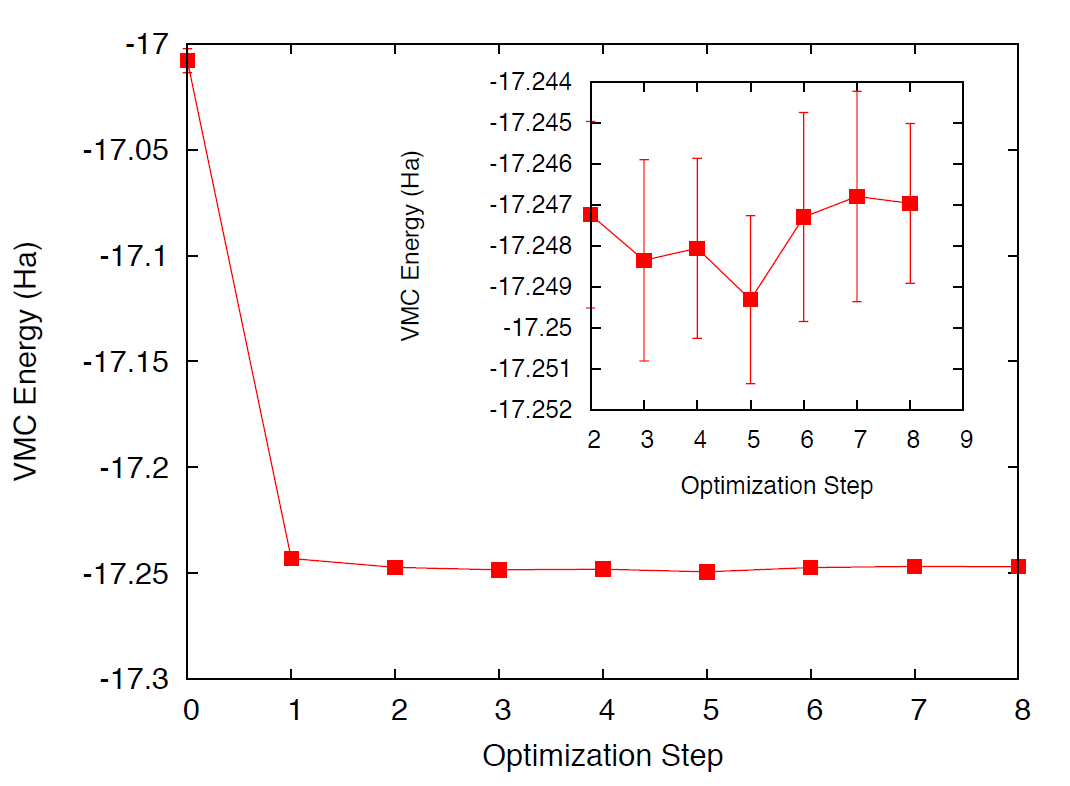
\includegraphics[trim = 0mm 0mm 0mm 0mm, clip,width=0.75\columnwidth]{./figures/lab_advanced_molecules_opt_conv}
\end{center}
\caption{VMC energy as a function of optimization step.
\label{fig:lam_opt_conv}
}
\end{figure}

The resulting energy as a function of optimization step should look qualitatively similar to figure \ref{fig:lam_opt_conv}.
The energy should decrease quickly as a function of the number of optimization steps. After 6-8 steps, the energy should be converged to $\sim$2-3mHa. To improve convergence,
we would need to increase the number of samples used during the optimization. You can
check this for yourself on your free time. With optimized wave-functions we are in a position
to perform VMC and DMC calculations. The modified wave-function files after each step
are written in a file named ID.sNNN.opt.xml, where ID is the identifier of the calculation
defined in the input file (this is defined in the project XML block with parameter “id”) and
NNN is a series number which increases with every executable xml block in the input file.


\subsection{Time-step Study}
Now we will study the dependence of the DMC energy with time-step. From the top directory, 
go to “ex1\_first-run-hartree-fock/dmc\_timestep”. This folder contains a basic xml input
file (dmc\_ts.xml) that performs a short VMC calculation and three DMC calculations
with varying time-steps (0.1, 0.05, 0.01). Link the particle set and the last optimization
file from the previous folder (the file called jopt-h2o.sNNN.opt.xml with the largest value of
NNN). Rename the optimized wave-function to any suitable name if you wish, for example
h2o.opt.xml, and change the name of the particle set and wave-function files in the
input file. An optimized wave-function can be found in the reference files (same location)
in case it is needed. %Using the submission script of the previous exercise as a base, create a
%submission script for this step and submit the run. Set the number of nodes to 32 (2 places
%must be changed), the number of threads to 16 and leave the number of tasks at 1.

The main steps needed to perform this exercise are:
\begin{shaded}
\begin{verbatim}
cd ${TRAINING TOP}/ex1_first-run-hartree-fock/dmc_timestep
cp ../opt/h2o.ptcl.xml ./
cp ../opt/jopt-h2o.s007.opt.xml h2o.opt.wfs.xml
# edit dmc_ts.xml to include the correct ptcl.xml and wfs.xml
jobrun_vesta qmcpack dmc_ts.xml
\end{verbatim}
\end{shaded}
While these runs complete, go to section D and review the basic VMC and DMC input
blocks. Notice that in the current DMC blocks, as the time-step is decreased the number of blocks is also increased. Why is this?

When the simulations are finished, use qmca to analyze the output files and to plot the
DMC energy as a function of time-step. Results should be qualitatively similar to those
presented in figure \ref{fig:lam_dmc_timestep}, in this case we present more time-steps with well converged results to
better illustrate the time-step dependence. In realistic calculations, the time-step must be
chosen small enough so that the resulting error is below the desire accuracy. Alternatively,
various calculations can be performed and the results extrapolated to the zero time-step
limit.


\begin{figure}
\begin{center}
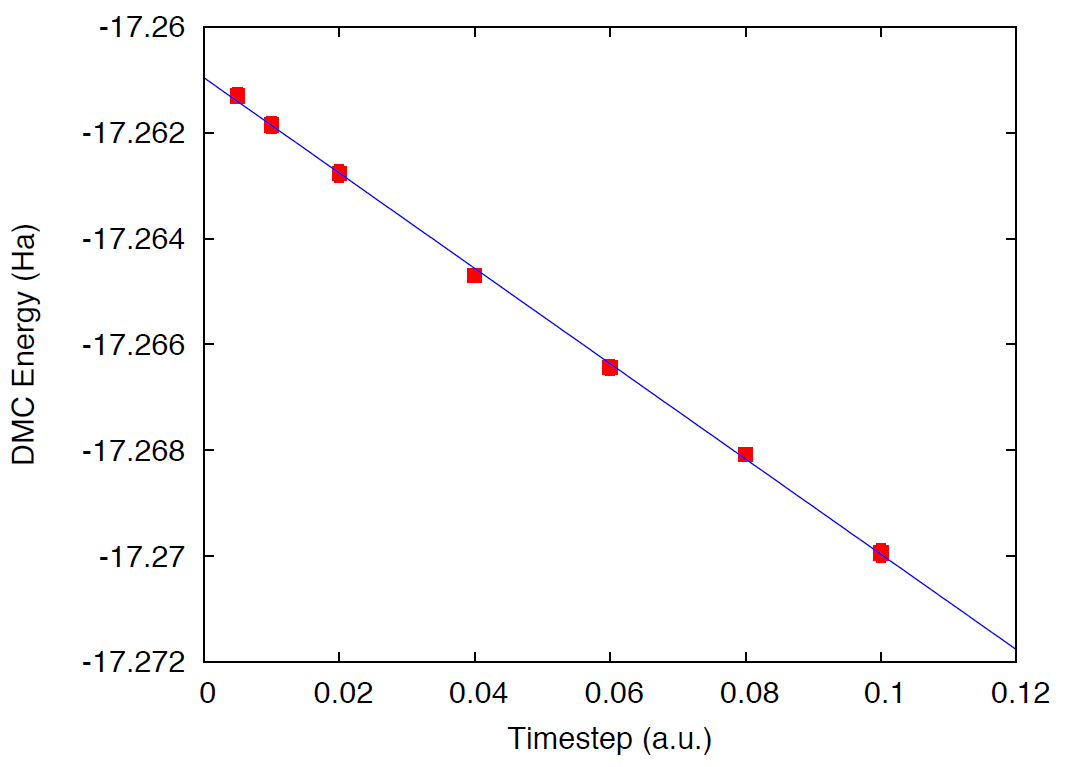
\includegraphics[trim = 0mm 0mm 0mm 0mm, clip,width=0.75\columnwidth]{./figures/lab_advanced_molecules_dmc_timestep}
\end{center}
\caption{DMC energy as a function of timestep.
\label{fig:lam_dmc_timestep}
}
\end{figure}


\subsection{Walker Population Study}
Now we will study the dependence of the DMC energy with the number of walkers in the
simulation. Remember that, in principle, the DMC distribution is reached in the limit of
an infinite number of walkers. In practice, the energy and most properties converge to high
accuracy with $\sim$100-1000 walkers. The actual number of walkers needed in a calculation
will depend on the accuracy of the VMC wave-function and on the complexity and size of
the system. Also notice that using too many walkers is not a problem, at worse it will be
inefficient since it will cost more computer time than necessary. In fact, this is the strategy
used when running QMC calculations on large parallel computers since we can reduce the
statistical error bars efficiently by running with large walker populations distributed across
all processors.

From the top directory, go to ``ex1\_first-run-hartree-fock/dmc\_walkers''. Copy the
optimized wave-function and particle set files used in the previous calculations to the current
folder, these are the ones generated on step 2 of this exercise. An optimized wave-function can be found in the reference files (same location) in case it is needed. The directory
contains a sample DMC input file and submission script. Make 3 directories named NWx,
with x values 120,240,480 and copy the input file to each one. Go
to ``NW120'', and, in the input file, change the name of the wave-function and particle set
files (in this case they will be located one directory above, so use ``../dmc\_timestep/h2.opt.xml'' for
example), change the pseudopotential directory to point to one directory above, change ``targetWalkers'' to 120, change the number of steps to 100, the time-step
to 0.04 and the number of blocks to 400. Notice that ``targetWalkers'' is one way to set the
desired (average) number of walkers in a DMC calculation.   For your own simulations we generally recommend setting $\sim$2*(\#threads)
walkers per node (slightly smaller than this value).

\begin{figure}
\begin{center}
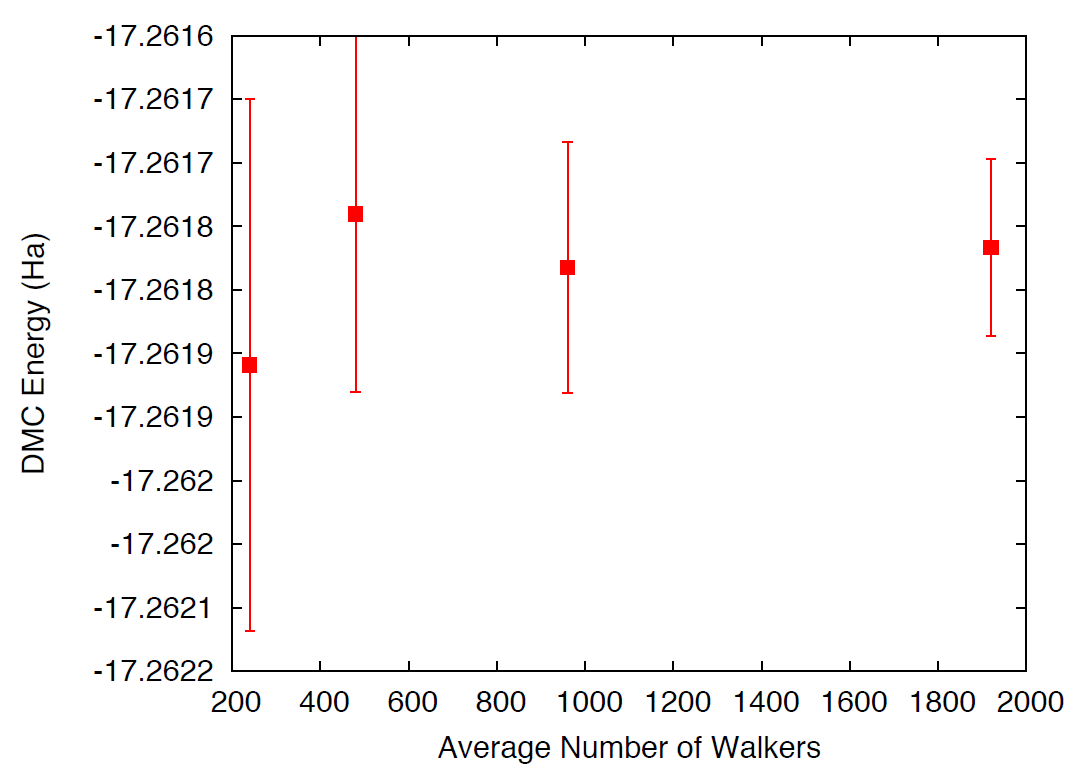
\includegraphics[trim = 0mm 0mm 0mm 0mm, clip,width=0.75\columnwidth]{./figures/lab_advanced_molecules_dmc_popcont}
\end{center}
\caption{DMC energy as a function of the average number of walkers.
\label{fig:lam_dmc_popcont}
}
\end{figure}

Repeat the same procedure in the other folders by setting (targetWalkers=240,
steps=100, timestep=0.04, blocks=200) in NW240 and (targetWalkers=480, 
steps=100, timestep=0.04, blocks=100) in NW480. When
the simulations complete, use qmca to analyze and plot the energy as a function of the
number of walkers in the calculation. As always, figure \ref{fig:lam_dmc_popcont} 
shows representative results of the
dependence of the energy on the number of walkers for a single water molecule. As shown,
less than 240 walkers are needed to obtain an accuracy of 0.1 mHa.


\section{Exercise \#2 Slater-Jastrow Wave-Function Options}
From this point on in the tutorial we assume familiarity with the basic parameters in the
optimization, VMC and DMC XML input blocks of QMCPACK. In addition, we assume
familiarity with the submission system. As a result, the folder structure will not contain
any prepared input or submission files, the student will generate them using generic versions
provided in ``QMCPACK/Generic Files'' and ``GAMESS/Generic Files''. In the case of QMCPACK sample 
files, you will find optm.xml, vmc dmc.xml and submit.csh files. Some of
the options in these files can be left unaltered, but many of them will need to be tailored to
the particular calculation.

In this exercise we will study the dependence of the DMC energy on the choices made
in the wave-function ansatz. In particular, we will study the influence/dependence of the
VMC energy with the various terms in the Jastrow. We will also study the influence of
the VMC and DMC energies on the single particle orbitals used to form the Slater determinant 
in single determinant wave-functions. For this we will use wave-functions generated
with various exchange-correlation functionals in DFT. Finally, we will optimize a simple
multi-determinant wave-function and study the dependence of the energy o the number of
configurations used in the expansion. All of these exercises will be performed on the water 
molecule at equilibrium.


\subsection{Influence of Jastrow on VMC energy with HF wave-function}
In this section we will study the dependence of the VMC energy on the various Jastrow
terms, e.g. one-body, two-body and three-body. From the top directory, go to ``ex2\_slater-jastrow-wf-options/jastrow''. 
We will compare the single determinant VMC energy using a two-body 
Jastrow term, both one- and two-body terms and finally one-, two- and three-body
terms. Since we are interested in the influence of the Jastrow, we will use the HF orbitals
calculated in exercise \#1. Make three folders named 2j,12j,123j. For both 2j and
12j %(we have already optimized a wave-function for the 1-2-3J case, so the steps will be
%slightly different in this case)
, copy the input file optm.xml %and the sample submission file
from ``ex1\_first-run-hartree-fock/opt'' . This input file performs both wave-function optimization 
and a VMC calculation. Copy the un-optimized HF wave-function and particle set files
from ``ex1\_first-run-hartree-fock/convert'', if you followed the instructions in exercise \#1 these should be
named h2o.wfs.xml and h2o.ptcl.xml. Otherwise, you can obtained them from the
REFERENCE files. Modify the file h2o.wfs.xml to remove the appropriate jastrow
blocks. For example, for a two-body Jastrow (only), you need to eliminate the jastrow
blocks named \texttt{<jastrow name="J1"} and \texttt{<jastrow name="J3"}. In the case of 12j, remove
only \texttt{<jastrow name="J3"}. Recommended settings for the optimization run are: nodes=32,
threads=16, blocks=250, samples=128000, time-step=0.5, 8 optimization loops, and in the
VMC section we recommend walkers=16, blocks=1000, steps=1, substeps=100. Notice that
samples should always be set to blocks*threads per node*nodes = 32*16*250=128000. Repeat 
the process in both 2j and 12j cases. For the 123j case, the wave-function has
already been optimized in the previous exercise. Copy the optimized HF wave-function and
the particle set from ``ex1\_first-run-hartree-fock/opt''. Copy the input file from any of the previous runs and remove the optimization block from the
input, just leave the VMC step. In all three cases, modify the submission script and submit the run.

\begin{figure}
\begin{center}
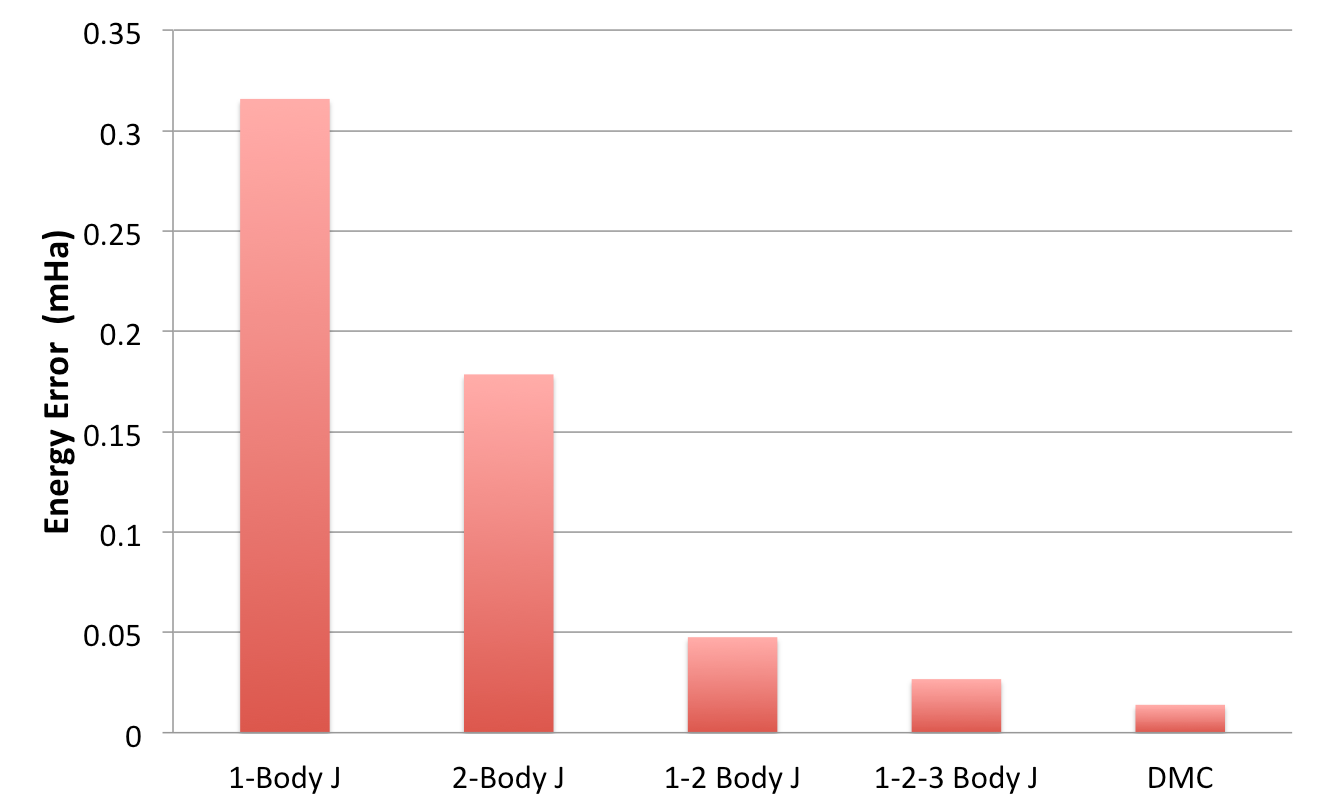
\includegraphics[trim = 0mm 0mm 0mm 0mm, clip,width=0.75\columnwidth]{./figures/lab_advanced_molecules_vmc_jastrow}
\end{center}
\caption{VMC energy as a function of Jastrow type.
\label{fig:lam_vmc_jastrow}
}
\end{figure}

These simulations will take several minutes to complete. This is an excellent opportunity
to go to section E and review the wavefunction XML block used by QMCPACK. When the
simulation are completed, use qmca to analyze the output files. Using your favorite plotting
program (e.g. gnu plot), plot the energy and variance as a function of the Jastrow form.
Figure \ref{fig:lam_vmc_jastrow} shows a typical result for this calculation. As can be seen, the VMC energy and
variance depends strongly on the form of the Jastrow. Since the DMC error bar is directly
related to the variance of the VMC energy, improving the Jastrow will always lead to a
reduction in the DMC effort. In addition, systematic approximations (time-step, number of
walkers, etc) are also reduced with improved wave-functions.


\subsection{Generation of wave-functions from DFT using GAMESS}
In this section we will use GAMESS to generate wave-functions for QMCPACK from
DFT calculations. From the top folder, go to ``ex2\_slater-jastrow-wf-options/orbitals''. In order to demonstrate
the variation in DMC energies with the choice of DFT orbitals, we will choose the following
set of exchange-correlation functionals (PBE, PBE0, BLYP, B3LYP). For each functional,
make a directory using your preferred naming convention (e.g. the name of the functional).
Go into each folder and copy a generic GAMESS input file from %for a ROHF calculation from
``ex1\_first-run-hartree-fock/gms'' .%, a file named rohf.inp should exist.
Rename the file with your preferred naming convention, we suggest using h2o.[dft].inp, where [dft] is the name of
the functional used in the calculation. At this point, this input file should be identical to the
one used to generate the HF wave-function in exercise \#1. In order to perform a DFT
calculation we only need to add ``DFTTYP'' to the \texttt{\$CONTRL ... \$END} section and set
it to the desired functional type, for example ``DFTTYP=PBE'' for a PBE functional. This
variable must be set to (PBE, PBE0, BLYP, B3LYP) to obtain the appropriate functional in
GAMESS. For a complete list of implemented functionals, see the GAMESS input manual.


\subsection{Optimization and DMC calculations with DFT wave-functions}
In this section we will optimize the wave-function generated in the previous step and
perform DMC calculations. From the top directory, go to “ex2\_slater-jastrow-wf-options/orbitals”.
The steps required to achieve this are identical to those used to optimize the wave-function
with HF orbitals. Make individual folders for each calculation and obtain the necessary files
to perform optimization, VMC and DMC calculations from ``ex1\_first-run-hartree-fock/opt'' and ``ex1\_first-run-hartree-fock/dmc\_ts'', for example.
%A file named optm vmc dmc.xml should exist that contains all three execution blocks. 
For each functional, make the appropriate modifications to the input files and copy the particle 
set and wave-function files from the appropriate directory in “ex2\_slater-jastrow-wf-options/orbitals/[dft]”. We
recommend the following settings: nodes=32, threads=16, (in optimization) blocks=250,
samples=128000, timestep=0.5, 8 optimization loops, (in VMC) walkers=16, blocks=100,
steps=1, substeps=100, (in DMC) blocks 400, targetWalkers=960, timestep=0.01. Submit
the runs and analyze the results using qmca .

How do the energies compare against each other? How do they compare against DMC
energies with HF orbitals?
%Orbital Sets and Configurations in 
\section{Exercise \#3: Multi-Determinant Wave-Functions}
In this exercise we will study the dependence of the DMC energy on the set of orbitals
and the type of configurations included in a multi-determinant wave-function. 

\subsection{Generation of a CISD wave-functions using GAMESS}
In this section we will use GAMESS to generate a multi-determinant wave-function with
Configuration Interaction with Single and Double excitations (CISD). In CISD, the Schrodinger equation is solved exactly in a basis of determinants 
including the HF determinant and all its single and double excitations. 

Go to ``ex3\_multi-slater-jastrow/cisd/gms'' and you'll see input and output files named h2o.cisd.inp and h2o.cisd.out. Due to technical problems with GAMESS in the BGQ architecture of VESTA, we are unable to use CISD properly in GAMESS. For this reason, the output of the calculation is  already provided in the directory. 

%You'll see several input and output files named h2o.XXX.inp
%and h2o.XXX.out, where XXX is one of the following multi-determinant methods: CISD,
%CASSCF, CASCI, SOCI. 

There will be time in the next step to study the GAMESS input
files and the description in section A. %In the next exercise we will use the CISD output, in
%the next exercise we will use the remaining files. 
Since the output is already provided, the
only thing needed is to use the converter to generate the appropriate QMCPACK files.  %Copy a submission script from GAMESS/Generic Files and execute the converter for all the output 
%files in the directory (with the exception of CASSCF, which is used to generate orbitals).
%but it doesn’t contain appropriate CI coefficients). 
\begin{shaded}
\begin{verbatim}
jobrun_vesta convert4qmc h2o.cisd.out -ci h2o.cisd.out \
-readInitialGuess 57 -threshold 0.0075
\end{verbatim}
\end{shaded}

We used the PRTMO=.T. flag in the GUESS section, to include orbitals in the output file. You should read these orbitals from the output (-readInitialGuess 40).
The highest occupied orbital in any determinant should be 34, so reading 40 orbitals is a safe choice. In this case, it is important to rename the xml files with meaningful names, for example h2o.cisd.wfs.xml. A threshold of 0.0075 is sufficient for the calculations in the training.


\subsection{Optimization of Multi-Determinant wave-function}

In this section we will optimize the wave-function generated in the previous step. There
is no difference in the optimization steps if a single determinant and a multi-determinant wave-function.
QMCPACK will recognize the presence of a multi-determinant wavefunction and will automatically 
optimize the linear coefficients by default. Go to ``ex3\_multi-slater-jastrow/cisd'' and make a folder called 
thres0.01. Copy the particle set and wavefunction files created in the previous step to the current 
directory. With your favorite text editor, open the wave-function file h2o.wfs.xml. Look for 
the multideterminant XML block and change the ``cutoff'' parameter in detlist to 0.01. Then follow 
the same steps used in the subsection ``Optimization and DMC calculations with DFT wave-functions''
to optimize the wave-function. Similar to this case, design a QMCPACK input file that performs
wave-function optimization followed by VMC and DMC calculations. Submit the calculation.

This is a good time to review the GAMESS input file description in Appendix section A. 
When the run is completed, go to the previous directory and make a new folder named
thres0.0075. Repeat the steps performed above to optimize the wave-function with a cutoff of 0.01, but use a cutoff of 0.0075 this time. This will increase the number of determinants used in the calculation. Notice the ``cutoff'' parameter in the XML should be less than the ``-threshold 0.0075'' flag passed to the converted, which is further bounded by the PRTTOL flag in the GAMESS input.

After the wave-function is generated, we are ready to optimize. Instead of starting from an un-optimized wave-function, we can start from optimized wave-function from thres0.01 to speed up convergence. You will need to modify the file and change the cutoff in detlist to 0.0075 with a text editor. Repeat the optimization steps and submit the calculation.

\begin{figure}
\begin{center}
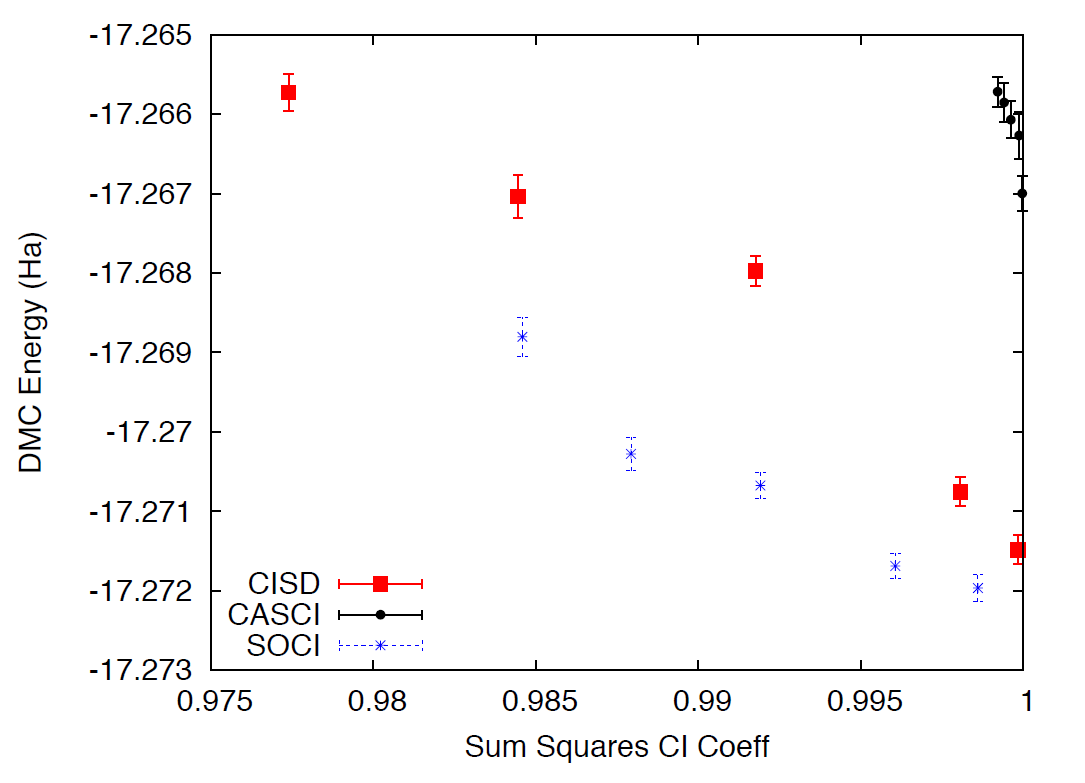
\includegraphics[trim = 0mm 0mm 0mm 0mm, clip,width=0.75\columnwidth]{./figures/lab_advanced_molecules_dmc_ci_cisd}
\end{center}
\caption{DMC energy as a function of the sum of the square of CI coefficients from CISD.
\label{fig:lam_dmc_ci_cisd}
}
\end{figure}

When you are done, use qmca to analyze the results. Compare the energies at these two
coefficient cutoffs with the energies obtained with DFT orbitals. Due to the time limitations of this tutorial it is not practical to optimize the wave-functions with a smaller cutoff, since this would require more samples and longer runs due to the larger number of optimizable parameters. Figure \ref{fig:lam_dmc_ci_cisd} shows the results of such exercise, the DMC energy as a function of the cutoff in the wave-function. As can be seen, a large improvement in the energy is obtained as the number of configurations is increased.


%Since the un-optimized wave-functions were generated in subsection “Generation of a CISD wavefunctions 
%using GAMESS” of exercise \#2, we can skip this section and go straight to the
%wave-function optimization. 

\subsection{CISD, CASCI and SOCI}

Go to “ex3\_multi-slater-jastrow” and inspect folders for the remaining wave-function types: CASCI and SOCI. Follow steps in the previous exercise and obtain the optimized wave-functions for these determinant choices. Notice the SOCI GAMESS output is not included because it is large. Already converted XML inputs can be found in ``ex3\_multi-slater-jastrow/soci/thres*''. %The exercise has already been performed with a CISD wave-function in exercise \#2.

A CASCI wave-function is produced from a CI calculation that includes all the determinants 
in a complete active space (CAS) calculation, in this case using the orbitals from a previous CASSCF
calculation. In this case we used a CAS(8,8) active space, that includes all determinants
generated by distributing 8 electrons in the lowest 8 orbitals. A second-order CI (SOCI) calculation is similar
to the CAS-CI calculation, but in addition to the determinants in the CAS it also includes
all single and double excitations from all of them, leading to a much larger determinant
set. Since we now have considerable experience optimizing wave-functions and calculating
DMC energies, we will leave it to the student to complete the remaining tasks on its own.
If you need help, refer to previous exercises in the tutorial. Perform optimizations for both
wave-functions using cutoffs in the CI expansion of 0.01 an 0.0075. If there is enough time
left, try to optimize the wave-functions with a cutoff of 0.005. Analyze the results and plot
the energy as a function of cutoff for all three cases, CISD, CAS-CI and SOCI.

Figure  \ref{fig:lam_dmc_ci_cisd} shows the result of similar calculations using more samples and smaller cutoffs.
The results should be similar to those produced in the tutorial. For reference, the exact
energy of the water molecule with ECPs is approximately -17.276 Ha. From the results of the
tutorial, how does the selection of determinants is related to the expected DMC energy?
What about the choice in the set of orbitals?


\newpage
\section{Appendix A: GAMESS input}
In this section we provide a brief description of the GAMESS input needed to produce
trial wave-function for QMC calculations with QMCPACK. We assume basic familiarity
with GAMESS input structure, in particular regarding the input of atomic coordinates and
the definition of gaussian basis sets. This section will focus on the generation of the output
files needed by the converter tool, convert4qmc. For a description of the converter, see B.

Only a subset of the methods available in GAMESS can be used to generate wave-functions 
for QMCPACK and we restrict our description here to these.
For a complete description of all the options and methods available
in GAMESS, please refer to the official documentation which could be found in
”http://www.msg.ameslab.gov/gamess/documentation.html”.

Currently, convert4qmc can process output for the following methods in GAMESS (in
SCFTYP) : RHF, ROHF, and MCSCF. Both HF as well as DFT calculations (any DFT
type) could be used in combination with RHF and ROHF calculations. For MCSCF and CI
calculations, ALDET, ORMAS and GUGA drivers can be used (see below for details).


\subsection{HF input}
The following input will perform a restricted HF calculation on a closed-shell singlet 
(multiplicity=1). This will generate RHF orbitals for any molecular system defined in 
\texttt{\$DATA ... \$END}.

\begin{lstlisting}
$CONTRL SCFTYP=RHF RUNTYP=ENERGY MULT=1
ISPHER=1 EXETYP=RUN COORD=UNIQUE MAXIT=200 $END
$SYSTEM MEMORY=150000000 $END
$GUESS GUESS=HUCKEL $END
$SCF DIRSCF=.TRUE. $END
$DATA
...
Atomic Coordinates and basis set
...
$END
\end{lstlisting}

Main options:
\begin{enumerate}
  \item{SCFTYP: Type of SCF method, options: RHF, ROHF, MCSCF, UHF and NONE.}
  \item{RUNTYP: Type of run. For QMCPACK wave-function generation this should always be ENERGY.}
  \item{MULT: Multiplicity of the molecule.}
  \item{ISPHER: Use spherical harmonics (1) or cartesian basis functions (-1).}
  \item{COORD: Input structure for the atomic coordinates in \$DATA.}
\end{enumerate}


\subsection{DFT calculations}
The main difference between the input for a RHF/ROHF calculation and a DFT calculation 
is the definition of the DFTTYP parameter. If this is set in the \$CONTROL
section, a DFT calculation will be performed with the appropriate functional. Notice that
while the default values are usually adequate, DFT calculations have many options involving
the integration grids and accuracy settings. Make sure you study the input manual to be
aware of these. Refer to the input manual for a list of the implemented exchange-correlation
functionals.


\subsection{Multi-Configuration Self-Consistent Field (MCSCF)}
MCSCF calculations are performed by setting SCFTYP=MCSCF in the $CONTROL
section. If this option is set, a $MCSCF section must be added to the input file with the
options for the calculation. An example section for the water molecule used in the tutorial
is shown below.

\begin{lstlisting}
$MCSCF CISTEP=GUGA MAXIT=1000 FULLNR=.TRUE. ACURCY=1.0D-5 $END
\end{lstlisting}

The most important parameter is CISTEP, which defines the CI package used. The only
options compatible with QMCPACK are: ALDET, GUGA, and ORMAS. Depending on the
package used, additional input sections are needed.


\subsection{Configuration Interaction (CI)}
Configuration interaction (full CI, truncated CI, CAS-CI, etc) calculations are performed
by setting SCFTYP=NONE and CITYP=GUGA,ALDET,ORMAS. Each one of this packages 
requires further input sections, which are typically slightly different to the input sections
needed for MCSCF runs.


\subsection{GUGA: Unitary Group CI package}
The GUGA package is the only alternative if one wants CSFs with GAMESS. Below
we provide a very brief description of input sections needed to perform MCSCF, CASCI,
truncated CI and SOCI with this package. For a complete description of these methods and
all the options available, please refer to the GAMESS input manual.

\subsubsection{GUGA-MCSCF}
The following input section performs a CASCI calculation, with a CAS that includes 8
electrons in 8 orbitals (4 DOC and 4 VAL), e.g. CAS(8,8). NMCC is the number of frozen
orbitals (doubly occupied orbitals in all determinants), NDOC is the number of double
occupied orbitals in the reference determinant, NVAL is the number of singly occupied
orbitals in the reference (for spin polarized cases), and NVAL is the number of orbitals in
the active space. Since FORS is set to .TRUE., all configurations in the active space will
be included. ISTSYM defines the symmetry of the desired state.

\begin{lstlisting}
$MCSCF CISTEP=GUGA MAXIT=1000 FULLNR=.TRUE. ACURCY=1.0D-5 $END
$DRT GROUP=C2v NMCC=0 NDOC=4 NALP=0 NVAL=4 ISTSYM=1 MXNINT= 500000 FORS=.TRUE. $END
\end{lstlisting}

\subsubsection{GUGA-CASCI}
The following input section performs a CASCI calculation, with a CAS that includes 8
electrons in 8 orbitals (4 DOC and 4 VAL), e.g. CAS(8,8). NFZC is the number of frozen
orbitals (doubly occupied orbitals in all determinants). All other parameters are identical
to those in the MCSCF input section.

\begin{lstlisting}
$CIDRT GROUP=C2v NFZC=0 NDOC=4 NALP=0 NVAL=4 NPRT=2 ISTSYM=1 FORS=.TRUE. MXNINT= 500000 $END
$GUGDIA PRTTOL=0.001 CVGTOL=1.0E-5 ITERMX=1000 $END
\end{lstlisting}

\subsubsection{GUGA-Truncated CI}
The following input sections will lead to a truncated CI calculation, in this particular case
it will perform a CISD calculation since IEXCIT is set to 2. Other values in IEXCIT will lead
to different CI truncations, for example IEXCIT=4 will lead to CISDTQ. Notice that only
the lowest 30 orbitals will be included in the generation of the excited determinants in this
case. For a full CISD calculation, NVAL should be set to the total number of virtual orbitals.

\begin{lstlisting}
$CIDRT GROUP=C2v NFZC=0 NDOC=4 NALP=0 NVAL=30 NPRT=2 ISTSYM=1 IEXCIT=2 MXNINT= 500000 $END
$GUGDIA PRTTOL=0.001 CVGTOL=1.0E-5 ITERMX=1000 $END
\end{lstlisting}

\subsubsection{GUGA-SOCI}
The following input section performs a SOCI calculation, with a CAS that includes 8
electrons in 8 orbitals (4 DOC and 4 VAL), e.g. CAS(8,8). Since SOCI is set to .TRUE.,
all single and double determinants from all determinants in the CAS(8,8) will be included.

\begin{lstlisting}
$CIDRT GROUP=C2v NFZC=0 NDOC=4 NALP=0 NVAL=4 NPRT=2 ISTSYM=1 SOCI=.TRUE. NEXT=30 MXNINT= 500000 $END
$GUGDIA PRTTOL=0.001 CVGTOL=1.0E-5 ITERMX=1000 $END
\end{lstlisting}


\subsection{ECP}
To use Effective Core Potentials (ECP) in GAMESS, you must define a \{\texttt{\$ECP ... \$END}\} 
block. There must be a definition of a potential for every atom in the system, including
symmetry equivalent ones. In addition, they must appear in the particular order expected
by GAMESS. Below is an example of an ECP input block for a single water molecule using
BFD ECPs. To turn on the use of ECPs, the option “ECP=READ” must be added to the
CONTROL input block.

\begin{lstlisting}
$ECP
O-QMC GEN 2 1
3
6.00000000 1 9.29793903
55.78763416 3 8.86492204
-38.81978498 2 8.62925665
1
38.41914135 2 8.71924452
H-QMC GEN 0 0
3
1.000000000000 1 25.000000000000
25.000000000000 3 10.821821902641
-8.228005709676 2 9.368618758833
H-QMC
$END
\end{lstlisting}


\newpage
\section{Appendix B: convert4qmc}
To generate the particleset and wavefunction XML blocks required by QMCPACK in
calculations with molecular systems, the converter convert4qmc must be used. The converter
will read the standard output from the appropriate Quantum Chemistry calculation and will
generate all the necessary input for QMCPACK. Below we describe the main options of the
converter for GAMESS output. In general, there are 3 ways to use the converter depending
on the type of calculation performed. The minimum syntax for each option is found below.
For a description of the xml files produced by the converter, see section E.

\begin{enumerate}
  \item{For all single determinant calculations (HF and DFT with any DFTTYP):}
  \begin{shaded}
  \begin{verbatim}
    convert4qmc -gamessAscii single det.out
  \end{verbatim}
  \end{shaded}
  \begin{itemize}
    \item{single det.out is the standard output generated by GAMESS.}
  \end{itemize}
  \item{\textit{(This option is not recommended. Use option below to avoid mistakes.)} For 
    multi-determinant calculations where the orbitals and configurations are read from different
    files (for example when using orbitals from a MCSCF run and configurations from a
    subsequent CI run):}
  \begin{shaded}
  \begin{verbatim}
    convert4qmc -gamessAscii orbitals multidet.out -ci cicoeff multidet.out
  \end{verbatim}
  \end{shaded}
  \begin{itemize}
    \item{orbitals\_multidet.out is the standard output from the calculation that generates the
       orbitals. cicoeff multidet.out is the standard output from the calculation that calculates 
       the CI expansion.}
  \end{itemize}
  \item{For multi-determinant calculations where the orbitals and configurations are read from
    the same file, using PRTMO=.T. in the GUESS input block:}
  \begin{shaded}
  \begin{verbatim}
    convert4qmc -gamessAscii multi det.out -ci multi det.out -readInitialGuess Norb
  \end{verbatim}
  \end{shaded}
  \begin{itemize}
    \item{multi\_det.out is the standard output from the calculation that calculates the CI expansion.}
  \end{itemize}
\end{enumerate}

Options:
\begin{itemize}
\item{\textbf{-gamessAscii file.out}: Standard output of GAMESS calculation. With the exception 
of determinant configurations and coefficients in multi-determinant calculations,
everything else is read from this file including: atom coordinates, basis sets, single
particle orbitals, ECPs, number of electrons, multiplicity, etc.}

\item{\textbf{-ci file.out}: In multi-determinant calculations, determinant configurations and 
coefficients are read from this file. Notice that single particle orbitals are NOT read
from this file. Recognized CI packages are: ALDET, GUGA and ORMAS. Output
produced with the GUGA package MUST have the option “NPRT=2” in the CIDRT
or DRT input blocks.}

\item{\textbf{-threshold cutoff}: Cutoff in multi-determinant expansion. Only configurations with
coefficients above this value are printed.}

\item{\textbf{-zeroCI}: Sets to zero the CI coefficients of all determinants, with the exception of the
first one.}

\item{\textbf{-readInitialGuess Norb}: Reads Norb initial orbitals (“INITIAL GUESS ORBITALS”) 
from GAMESS output. These are orbitals generated by the GUESS input
block and printed with the option “PRTMO=.T.”. Notice that this is useful only in
combination with the option “GUESS=MOREAD” and in cases where the orbitals
are not modified in the GAMESS calculation, e.g. CI runs. This is the recommended
option in all CI calculations.}

\item{\textbf{-NaturalOrbitals Norb}: Read Norb “NATURAL ORBITALS” from GAMESS
output. The natural orbitals must exists in the output, otherwise the code aborts.}

\item{\textbf{-add3BodyJ}: Adds three-body Jastrow terms (e-e-I) between electron pairs (both
same spin and opposite spin terms) and all ion species in the system. The radial
function is initialized to zero and the default cutoff is 10.0 bohr. The converter will
add a one- and two-body Jastrow to the wavefunction block by default.}
\end{itemize}

Useful notes:
\begin{itemize}
  \item{The type of single particle orbitals read by the converter depends on the type of
calculation and on the options used. By default, when neither -readInitialGuess or
-NaturalOrbitals are used, the following orbitals are read in each case (notice that
-readInitialGuess or -NaturalOrbitals are mutually exclusive):}
  \begin{itemize}
    \item{RHF and ROHF: “EIGENVECTORS”}
    \item{MCSCF: “MCSCF OPTIMIZED ORBITALS”}
    \item{GUGA, ALDET, ORMAS: Cannot read orbitals without -readInitialGuess or -NaturalOrbitals options.}
  \end{itemize}
  \item{The single particle orbitals and printed CI coefficients in MCSCF calculations are
not consistent in GAMESS. The printed CI coefficients correspond to the next-to-last
iteration, they are not recalculated with the final orbitals. So in order to get appropriate 
CI coefficients from MCSCF calculations, a subsequent CI (no SCF) calculation
is needed to produce consistent orbitals. In principle, it is possible to read the orbitals 
from the MCSCF output and the CI coefficients and configurations from the
output of the following CI calculations. This could lead to problems in principle, since
GAMESS will rotate initial orbitals by default in order to obtain an initial guess consistent 
with the symmetry of the molecule. This last step is done by default and can
change the orbitals reported in the MCSCF calculation before the CI is performed.
In order to avoid this problem, it is highly recommended to use option \#3 above to
read all the information from the output of the CI calculation, this requires the use
of “PRTMO=.T.” in the GUESS input block. Since the orbitals are printed after any
symmetry rotation, the resulting output will always be consistent.}
\end{itemize}


\newpage
\section{Appendix C: Wave-function Optimization XML block}

%\FloatBarrier
\begin{figure}[ht!]
\begin{center}
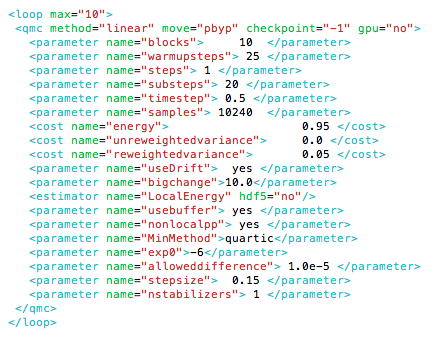
\includegraphics[trim = 0mm 0mm 0mm 0mm, clip,width=0.70\columnwidth]{./figures/lab_advanced_molecules_xml_opt}
\end{center}
\caption{Sample XML optimization block.
\label{fig:lam_xml_opt}
}
\end{figure}
%\FloatBarrier

Options:
\begin{itemize}
  \item{bigchange: (default 50.0) largest parameter change allowed}
  \item{usebuffer: (default no) Save useful information during VMC}
  \item{nonlocalpp: (default no) Include non-local energy on 1-D min}
  \item{MinMethod: (default quartic) Method to calculate magnitude of parameter change
quartic: fit quartic polynomial to 4 values of the cost function obtained using reweighting 
along chosen direction linemin: direct line minimization using reweighting rescale:
no 1-D minimization. Uses Umrigars suggestions.}
  \item{stepsize: (default 0.25) step size in either quartic or linemin methods.}
  \item{alloweddifference: (default 1e-4) Allowed increased in energy}
  \item{exp0: (default -16.0) Initial value for stabilizer (shift to diagonal of H) Actual value
of stabilizer is 10 exp0}
  \item{nstabilizers: (default 3) Number of stabilizers to try}
  \item{stabilizaterScale: (default 2.0) Increase in value of exp0 between iterations.}
  \item{max its: (default 1) number of inner loops with same sample}
  \item{minwalkers: (default 0.3) minimum value allowed for the ratio of effective samples
to actual number of walkers in a reweighting step. The optimization will stop if the
effective number of walkers in any reweighting calculation drops below this value. Last
set of acceptable parameters are kept.}
  \item{maxWeight: (defaul 1e6) Maximum weight allowed in reweighting. Any weight above
this value will be reset to this value.}
\end{itemize}

Recommendations:
\begin{itemize}
  \item{Set samples to equal to (\#threads)*blocks.}
  \item{Set steps to 1. Use substeps to control correlation between samples.}
  \item{For cases where equilibration is slow, increase both substeps and warmupsteps.}
  \item{For hard cases (e.g. simultaneous optimization of long MSD and 3-Body J), set exp0
to 0 and do a single inner iteration (max its=1) per sample of configurations.}
\end{itemize}


\newpage
\section{Appendix D: VMC and DMC XML block}

%\FloatBarrier
\begin{figure}[ht!]
\begin{center}
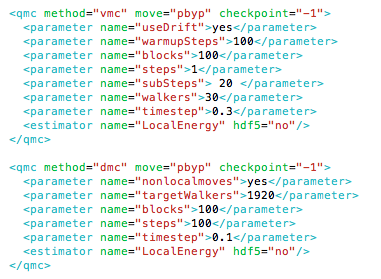
\includegraphics[trim = 0mm 0mm 0mm 0mm, clip,width=0.75\columnwidth]{./figures/lab_advanced_molecules_xml_vmc_dmc}
\end{center}
\caption{Sample XML blocks for VMC and DMC calculations.
\label{fig:lam_xml_vmc_dmc}
}
\end{figure}
%\FloatBarrier

General Options:
\begin{itemize}
\item{\textbf{move}: (default ”walker”) Type of electron move. Options: ”pbyp” and ”walker”.}
\item{\textbf{checkpoint}: (default ”-1”) (If ¿ 0) Generate checkpoint files with given frequency.
The calculations can be restarted/continued with the produced checkpoint files.}
\item{\textbf{useDrift}: (default ”yes”) Defines the sampling mode. useDrift = ”yes” will
use Langevin acceleration to sample the VMC and DMC distributions, while
useDrift=”no” will use random displacements in a box.}
\item{\textbf{warmupSteps}: (default 0) Number of steps warmup steps at the beginning of the
calculation. No output is produced for these steps.}
\item{\textbf{blocks}: (default 1) Number of blocks (outer loop).}
\item{\textbf{steps}: (default 1) Number of steps per blocks (middle loop).}
\item{\textbf{sub steps}: (default 1) Number of substeps per step (inner loop). During sub steps,
the local energy is not evaluated in VMC calculations, which leads to faster execution.
In VMC calculations, set sub steps to the average autocorrelation time of the desired
quantity.}
\item{\textbf{time step}: (default 0.1) Electronic time step in bohr.}
\item{\textbf{samples}: (default 0) Number of walker configurations saved during the current 
calculation.}
\item{\textbf{walkers}: (default \#threads) In VMC, sets the number of walkers per node. The total
number of walkers in the calculation will be equal to walkers*(\# nodes).}
\end{itemize}

Options unique to DMC:
\begin{itemize}
\item{\textbf{targetWalkers}: (default \#walkers from previous calculation, e.g. VMC.) Sets the
target number of walkers. The actual population of walkers will fluctuate around this
value. The walkers will be distributed across all the nodes in the calculation. On a
given node, the walkers are split across all the threads in the system.}
\item{\textbf{nonlocalmoves}: (default ”no”) Set to ”yes” to turns on the use of Casula’s T-moves.}
\end{itemize}


\newpage
\section{Appendix E: Wave-function XML block}

%\FloatBarrier
\begin{figure}[ht!]
\begin{center}
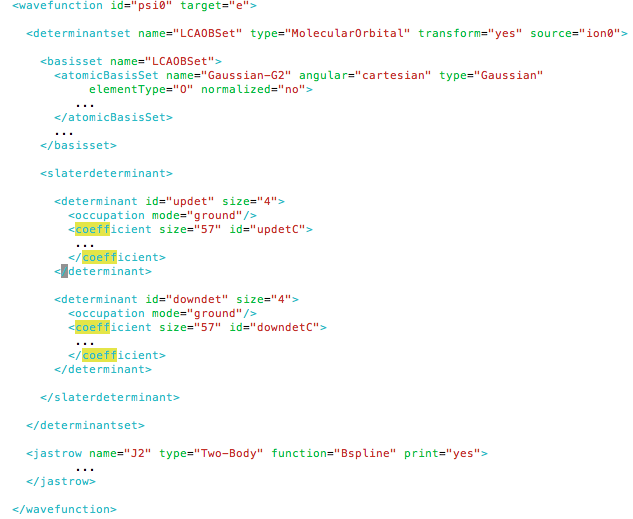
\includegraphics[trim = 0mm 0mm 0mm 0mm, clip,width=1.0\columnwidth]{./figures/lab_advanced_molecules_xml_determinantset}
\end{center}
\caption{Basic framework for a single determinant determinantset XML block.
\label{fig:lam_xml_determinantset}
}
\end{figure}
%\FloatBarrier

In this section we describe the basic format of a QMCPACK wavefunction XML block.
Everything listed in this section is generated by the appropriate converter tools. Little to
no modification is needed when performing standard QMC calculations. As a result, this
section is meant mainly for illustration purposes. Only experts should attempt to modify
these files (with very few exceptions like the cutoff of CI coefficients and the cutoff in Jastrow
functions) since changes can lead to unexpected results.

%\FloatBarrier
\begin{figure}[ht!]
\begin{center}
\includegraphics[trim = 0mm 0mm 0mm 0mm, clip,width=1.0\columnwidth]{./figures/lab_advanced_molecules_xml_basisset}
\end{center}
\caption{Sample XML block for an atomic orbital basis set.
\label{fig:lam_xml_basisset}
}
\end{figure}
%\FloatBarrier

A QMCPACK wavefunction XML block is a combination of a determinantset, which
contains the anti-symmetric part of the wave-function, and one or more jastrow blocks.
The syntax of the anti-symmetric block depends on whether the wave-function is a single
determinant or a multi-determinant expansion. Figure \ref{fig:lam_xml_determinantset} 
shows the general structure of the
single determinant case. The determinantset block is composed of a basisset block, which
defines the atomic orbital basis set, and a slaterdeterminant block, which defines the single
particle orbitals and occupation numbers of the Slater determinant. Figure \ref{fig:lam_xml_basisset} 
shows a section
of a basisset block for an oxygen atom. The structure of this block is rigid and should not
be modified. Figure \ref{fig:lam_xml_slaterdeterminant} shows a (piece of a) sample of a 
slaterdeterminant block. The
slaterdeterminant block consists of 2 determinant blocks, one for each electron spin. The
parameter “size” in the determinant block refers to the number of single particle orbitals
present while the “size” parameter in the coefficient block refers to the number of atomic
basis functions per single particle orbital.

%\FloatBarrier
\begin{figure}[ht!]
\begin{center}
\includegraphics[trim = 0mm 0mm 0mm 0mm, clip,width=1.0\columnwidth]{./figures/lab_advanced_molecules_xml_slaterdeterminant}
\end{center}
\caption{Sample XML block for the single slater determinant case.
\label{fig:lam_xml_slaterdeterminant}
}
\end{figure}
%\FloatBarrier

Figure \ref{fig:lam_xml_multideterminant} shows the general structure of the multi-determinant case. 
Similar to the
single determinant case, the determinantset must contain a basisset block. This definition is
identical to the one described above. In this case, the definition of the single particle orbitals
must be done independently from the definition of the determinant configurations, the latter
is done in the sposet block while the former is done on the multideterminant block. Notice
that 2 sposet sets must be defined, one for each electron spin. The name of reach sposet set
is required in the definition of the multideterminant block. The determinants are defined in
terms of occupation numbers based on these orbitals.

%\FloatBarrier
\begin{figure}[ht!]
\begin{center}
\includegraphics[trim = 0mm 0mm 0mm 0mm, clip,width=1.0\columnwidth]{./figures/lab_advanced_molecules_xml_multideterminant}
\end{center}
\caption{Basic framework for a multi-determinant determinantset XML block.
\label{fig:lam_xml_multideterminant}
}
\end{figure}
%\FloatBarrier

There are various options in the multideterminant block that users should be aware of.
\begin{itemize}
  \item{cutoff: (IMPORTANT! ) Only configurations with (absolute value) “qchem coeff”
larger than this value will be read by QMCPACK.}
  \item{optimize: Turn on/off the optimization of linear CI coefficients.}
  \item{coeff: (in csf ) Current coefficient of given configuration. Gets updated during 
wavefunction optimization.}
  \item{qchem coeff: (in csf ) Original coefficient of given configuration from GAMESS 
calculation. This is used when applying a cutoff to the configurations read from the file.
The cutoff is applied on this parameter and not on the optimized coefficient.}
  \item{nca and nab: number of core orbitals for up/down electrons. A core orbital is an
orbital that is doubly occupied in all determinant configurations, not to be confused
with core electrons. These are not explicitly listed on the definition of configurations.}
  \item{nea and neb: number of up/down active electrons (those being explicitly correlated).}
  \item{nstates: number of correlated orbitals}
  \item{size (in detlist ): contains the number of configurations in the list.}
\end{itemize}
The remaining part of the determinantset block is the definition of jastrow factor. Any
number of these can be defined. Figure \ref{fig:lam_xml_jastrow} shows a sample jastrow 
block including one-, two- and three-body terms. This is the standard block produced by 
convert4qmc with the option -add3BodyJ (this particular example is for a water molecule). 
Optimization of individual radial functions can be turned on/off using the “optimize” 
parameter. It can be added to any coefficients block, even though it is currently not 
present in the J1 and J2 blocks.

%\FloatBarrier
\begin{figure}[ht!]
\begin{center}
\includegraphics[trim = 0mm 0mm 0mm 0mm, clip,width=1.0\columnwidth]{./figures/lab_advanced_molecules_xml_jastrow}
\end{center}
\caption{Sample Jastrow XML block.
\label{fig:lam_xml_jastrow}
}
\end{figure}
%\FloatBarrier

This training assumes basic familiarity with the UNIX operating system. In particular,
we use simple scripts written in “csh”. In addition, we assume that the student has obtained
all the necessary files and executables, and that the location of the training files are located
at \$\{TRAINING TOP\}.

The goal of the training not only to familiarize the student with the execution and
options in QMCPACK, but also to introduce him/her to important concepts in quantum
Monte Carlo calculations and many-body electronic structure calculations.



\chapter{Lab 4: Using PWSCF and QMCPACK to perform total energy calculations of
condensed systems}

\begin{flushleft}
\textbf{Lab author: Luke Shulenburger}\footnote{Sandia National Laboratories is a multiprogram
laboratory managed and operated by Sandia Corporation, a wholly owned
subsidiary of Lockheed Martin Corporation, for the U.S. Department of Energy's
National Nuclear Security Administration under Contract No.
DE-AC04-94AL85000.}

\textbf{Creation date: July 17, 2014}
\end{flushleft}


The goal of this lab will be to introduce you to the somewhat specialized problems involved in performing diffusion Monte Carlo calculations on condensed matter as opposed to the atoms and molecules that were the focus of earlier labs.   Calculations will be performed on two different systems.  Firstly, we will perform a series of calculations on BCC beryllium focusing on the necessary methodology to limit finite size effects.  Secondly, we will perform calculations on graphene as an example of a system where qmcpack’s ability to handle cases with mixed periodic and open boundary conditions is useful.  This example will also focus on strategies to limit memory usage for such systems.
All of the calculations performed in this lab will utilize the project suite tools that vastly simplify the process by automating the steps of generating trial wavefunctions and performing DMC calculations.

\newcommand{\vp}{\mathbf{a}^\text{p}}
\newcommand{\vs}{\mathbf{a}^\text{s}} 
\newcommand{\Smat}{\mathbf{S}}
\section{Preliminaries}
For any DMC calculation, we must start with a trial wavefunction. As is typical for our calculations of condensed matter, we will produce this wavefunction using density functional theory.  Specifically, we will use quantum espresso to generate a slater determinant of single particle orbitals.  This is done as a three step process.  First, we calculate the converged charge density by performing a DFT calculation with a fine grid of k-points to fully sample the Brilloiun zone.  Next, a non-self consistent calculation is performed at the specific k-points needed for the supercell and twists needed in the DMC calculation (more on this later).  Finally, a wavefunction is converted from the binary representation used by quantum espresso to the portable hdf5 representation used by qmcpack.

The choice of k-points necessary to generate the wavefunctions dependes on both the supercell chosen for the DMC calculation and by the supercell twist vectors needed.  Recall that the wavefunction in a plane wave DFT calculation is written using Bloch's theorem as:
\begin{equation}
\Psi(\vec{r}) = e^{i\vec{k}\cdot\vec{r}}u(\vec{r})
\end{equation}
Where $\vec{k}$ is confined ot the first Brillouin zone of the cell chosen and $u(\vec{r})$ is periodic in this simulation cell.  A plane wave DFT calculation stores the periodic part of the wavefunction as a linear combination of plane waves for each single particle orbital at all k-points selected.  The symmetry of the system allows us to generate an arbitrary supercell of the primitive cell as follows:  Consider the set of primitive lattice vectors, $ \{ \mathbf{a}^p_1, \mathbf{a}^p_2,
\mathbf{a}^p_3\} $.  We may write these vectors in a matrix, $\mathbf{L}_p$, whose
rows are the primitive lattice vectors.  Consider a non-singular
matrix of integers, $\Smat$.  A corresponding set of supercell lattice
vectors, $\{\mathbf{a}^s_1, \mathbf{a}^s_2, \mathbf{a}^s_3\}$, can be constructed by the matrix
product 
\begin{equation}
\mathbf{a}^s_i = S_{ij} \mathbf{a}^p_j
\end{equation}
If the primitive cell contains $N_p$ atoms, the supercell will then
contain $N_s = |\det(\Smat)| N_p$ atoms.

Now, the wavefunciton at any point in this new supercell can be related to the wavefunction in the primitive cell by  finding the linear combination of primitive lattice vectors that maps this point back to the primitive cell:
\begin{equation}
\vec{r}' = \vec{r} + x \mathbf{a}^p_1 + y \mathbf{a}^p_2 + z\mathbf{a}^p_3 = \vec{r} + \vec{T}
\end{equation}
where $x, y, z$ are integers.   Now the wavefunction in the supercell at point $\vec{r}'$ can be written in terms of the wavefunction in the primitive cell at $\vec{r}'$ as:
\begin{equation}
\Psi(\vec{r}) = \Psi(\vec{r}') e^{i \vec{T} \cdot \vec{k}}
\end{equation}
where $\vec{k}$ is confined to the first Brillouin zone of the primitive cell.  We have also chosen the supercell twist vector which places a constraint on the form of the wavefunction in the supercell.  The combination of these two constraints allows us to identify family of N k-points in the primitive cell that satisfy the constraints.  Thus for a given supercell tiling matrix and twist angle, we can write the wavefunction everywhere in the supercell by knowing the wavefunction a N k-points in the primitive cell.  This means that the memory necesary to store the wavefunction in a supercell is only linear in the size of the supercell rather than the quadratic cost if symmetry were neglected.

\section{Total energy of BCC beryllium}

As was discussed in this morning’s lectures when performing calculations of periodic solids with QMC, it is essential to work with a reasonable size supercell rather than the primitive cells that are common in mean field calculations.  Specifically, all of the finite size correction schemes discussed in the morning require that the exchange-correlation hole be considerably smaller than the periodic simulation cell.  Additionally, finite size effects are lessened as the distance between the electrons in the cell and their periodic images increases, so it is advantageous to generate supercells that are as spherical as possible so as to maximize this distance.  However, there is a competing consideration in that for calculating total energies we often want to be able to extrapolate the energy per particle to the thermodynamic limit by means of the following formula in 3 dimensions:
\begin{equation}
E_{\inf} = C + E_{N}/N
\end{equation}
This formula derived assuming the shape of the supercells is consistent (more specifically that the periodic distances scale uniformly with system size), meaning we will need to do a uniform tiling, ie, 2x2x2, 3x3x3 etc.  As a 3x3x3 tiling is 27 times larger than the supercell and the practical limit of DMC is on the order of 200 atoms (depending on Z), sometimes it is advantagous to choose a less spherical supercell with fewer atoms rather than a more spherical one that is too expensive to tile.

In the case of a BCC crystal, it is possible to tile the one atom primitive cell to a cubic supercell by only doubling the number of electrons.  This is the best possible combination of a small number of atoms that can be tiled and a regular box that maximizes the distance between periodic images.  We will need to determine the tiling matrix S that generates this cubic supercell by solving the following equation for the coefficients of the S matrix:
\begin{equation}
 \left[\begin{array}{rrr}
  1 & 0 & 0 \\
  0 & 1 & 0 \\
  0 & 0 & 1 
  \end{array}\right] =  \left[\begin{array}{rrr}
  s_{11} & s_{12} & s_{13} \\
  s_{21} & s_{22} & s_{23} \\
  s_{31} & s_{32} & s_{33} 
  \end{array}\right] \cdot 
\left[\begin{array}{rrr}
  0.5 &  0.5 & -0.5 \\
 -0.5 &  0.5 &  0.5 \\
  0.5 & -0.5 &  0.5
\end{array}\right] 
\end{equation}

We will now use the project suite to generate the trial wavefunction for this BCC beryllium.

Fortunately, the project-suite will handle determination of the proper k-vectors given the tiling matrix.  All that is needed is to place the tiling matrix in the Be-2at-setup.py file.   Now the definition of the physical system is:

\begin{lstlisting}
    bcc_Be = generate_physical_system(
        lattice    = 'cubic',
        cell       = 'primitive',
        centering  = 'I',
        atoms      = 'Be',
        constants  = 3.490,
        units      = 'A',
        net_charge = 0,
        net_spin   = 0,
        Be         = 2,
        tiling     = [[a,b,c],[d,e,f],[g,h,i]],
        kgrid      = kgrid,
        kshift     = (.5,.5,.5)
        )
\end{lstlisting}
Where the tiling line should be replaced with the row major tiling matrix from above.  This script file will now perform a converged DFT calculation to generate the charge density in a directory called bcc-beryllium/scf and perform a non self consistend DFT calculation to generate single particle orbitals in the direcotry bcc-beryllium/nscf.  Fortunately, the project suite will calculate the required k-points needed to tile the wavefunction to the supercell, so all that is necessary is the granularity of the supercell twists and whether this grid is shifted from the origin.  Once this is finished, it performs the conversion from pwscf's binary format to the hdf5 format used by qmcpack.  Finally, it will optimize the coefficients of one-body and two-body jastrow factors in the supercell defined by the tiling matrix.

Run these calculations by executing the script Be-2at-setup.py.  You will notice that such small calcuations as are required to generate the wavefunction of Be in a one atom cell are rather inefficent to run on a high performance computer such as vesta in terms of the time spent doing calculations versus time waiting on the scheduler and booting compute nodes.  One of the benefits of the portable hdf format that is used by qmcpack is that you can generate data like wavefunctions on a local workstation or other convenient resource and only use high performance clusters for the more expensive QMC calculations.

In this case, the wavefunction is generated in the directory bcc-beryllium/nscf-2at\_222/pwscf\_output in a file called pwscf.pwscf.h5.  It can be useful for debugging purposes to be able to verify the contents of this file are what you expect.  For instance, you can use the tool h5ls to check the geometry of the cell where the dft calculations were performed, or number of k-points or electrons in the calculation.  This is done with the command: h5ls -d pwscf.pwscf.h5/supercell or h5ls -d pwscf.pwscf.h5/electrons.

In the course of running Be-2at-setup.py, you will get an error when attempting to perform the vmc and wavefunction optimization calculations.  This is due to the fact that the wavefunction has been generated supercell twists of the form (+/- 1/4, +/- 1/4, +/- 1/4).  In the case that the supercell twist contains only 0 or 1/2, it is possible to operate entirely with real arithmetic.  The executabe that has been indicated in Be-2at-setup.py has been compiled for this case.  Note that where this is possible, the memory usage is a factor of two less than the general case and the calculations are somewhat faster.  However, it is often necessary to perform calculations away from these special twist angles in order to reduce finite size effects.  To fix this, delete the directory bcc-beryllium/opt-2at, change the line in near the top of Be-2at-setup.py from 
\begin{lstlisting}
qmcpack    = '/soft/applications/qmcpack/build_XL_real/bin/qmcapp'
\end{lstlisting}
to
\begin{lstlisting}
qmcpack    = '/soft/applications/qmcpack/build_XL_complex/bin/qmcapp'
\end{lstlisting}
and rerun the script.

When the optimiztion calculation has finished, check that everything as proceeded correctly by looking at the output in the opt-2at directory.  Firstly, you can grep the output file for Delta to see if the cost function has indeed been decreasing during the optimization.  You should find something like:
\begin{lstlisting}
 OldCost: 4.8789147e-02 NewCost: 4.0695360e-02 Delta Cost:-8.0937871e-03
 OldCost: 3.8507795e-02 NewCost: 3.8338486e-02 Delta Cost:-1.6930674e-04
 OldCost: 4.1079105e-02 NewCost: 4.0898345e-02 Delta Cost:-1.8076319e-04
 OldCost: 4.2681333e-02 NewCost: 4.2356598e-02 Delta Cost:-3.2473514e-04
 OldCost: 3.9168577e-02 NewCost: 3.8552883e-02 Delta Cost:-6.1569350e-04
 OldCost: 4.2176276e-02 NewCost: 4.2083371e-02 Delta Cost:-9.2903058e-05
 OldCost: 4.3977361e-02 NewCost: 4.2865751e-02 Delta Cost:-1.11161830-03
 OldCost: 4.1420944e-02 NewCost: 4.0779569e-02 Delta Cost:-6.4137501e-04
\end{lstlisting}
Which shows that the starting wavefunction was fairly good and that most of the optimizaiton occurred in the first step.  Confirm this by using qmca to look at how the energy and variance changed over the course of the calculation with teh comand: qmca -q ev -e 10 *.scalar.dat executed in the opt-2at directory.  You should get output like the following:
\begin{lstlisting}
                 LocalEnergy               Variance             ratio
opt  series 0  -2.159139 +/- 0.001897   0.047343 +/- 0.000758   0.0219 
opt  series 1  -2.163752 +/- 0.001305   0.039389 +/- 0.000666   0.0182 
opt  series 2  -2.160913 +/- 0.001347   0.040879 +/- 0.000682   0.0189 
opt  series 3  -2.162043 +/- 0.001223   0.041183 +/- 0.001250   0.0190 
opt  series 4  -2.162441 +/- 0.000865   0.039597 +/- 0.000342   0.0183 
opt  series 5  -2.161287 +/- 0.000732   0.039954 +/- 0.000498   0.0185 
opt  series 6  -2.163458 +/- 0.000973   0.044431 +/- 0.003583   0.0205 
opt  series 7  -2.163495 +/- 0.001027   0.040783 +/- 0.000413   0.0189 
\end{lstlisting}

Now that the optimization has completed successfully, we can perform dmc calculations.  The first goal of the calculations will be to try to eliminate the one body finite size effects by twist averaging.  The script Be-2at-qmc.py has the necessary input.  Note on line 42 two twist grids are specified, (2,2,2) and (3,3,3).  Change the tiling matrix in this input file as in Be-2at-qmc.py and start the calculations.  Note that this workflow takes advantage of qmcpack's ability to group jobs.  If you look in the directory dmc-2at\_222 at the job submission script, (dmc.qsub.in) you will note that rather than operating on an xml input file, qmcapp is targeting a text file called dmc.in.  This file is a simple text file that contains the names of the 8 xml input files needed for this job, one for each twist.  When operated in this mode, qmcpack will use mpi groups to run multiple copies of itself within the same mpi context.  This is often useful both in terms of organizing calculations and also for taking advantage of the large job sizes that computer centers often encourage.

The dmc calculations in this case are designed to complete in a few minutes.  When they have finished running, first look at the scalar.dat files corresponding to the dmc calculations at the various twists in dmc-2at\_222.  Using a command like 'qmca -q ev -e 32 *.s001.scalar.dat' (with a suitably chosen number of blocks for the equilibration), you will see that the dmc energy in each calcuation is nearly identical within the statistical uncertainty of the calculations.  In the case of a large supercell, this is often indicative of a situation where the Brilloiun zone is so small that the one body finite size effects are nearly converged without any twist averaging.  In this case, however, this is because of the symmetry of the system.  For this cubic supercell, all of the twist angles chosen in this shifted 2x2x2 grid are equivalent by symmetry.  In the case where substantial resources are required to equilibrate the dmc calculations, it can be beneficial to avoid repeating such twists and instead simply weight them properly.  In this case however where the equilibration is inexpensive, there is no benefit to adding such complexity as the calculations can simply be averaged together and the result is equivalent to performing a single longer calcuation.

Using the command qmc -a -q ev -e 16 *.s001.scalar.dat, average the dmc energies in dmc-2at\_222 and dmc-2at\_333 to see whether the one body finite size effects are converged with a 3x3x3 grid of twists.  As beryllium as a metal, the convergence is quite poor (~0.025 Ha / Be or ~ 0.7 eV / Be).  If this were a production calculation it would be necessary to perform calculations on much larger grids of supercell twists to eliminate the one body finite size effects.

In this case there are several other calculations that would warrent a high priority.  A script Be-16at-qmc.py has been provided where you can imput the appropriate tiling matrix for a 16 atom cell and perform calculations to estimate the two body finite size effects which will also be quite large in the 2 atom calculations.  This script will take approximately 30 minutes to run to completion, so depending on interest,  you can either run it, or also work to modify the scripts to address the other technical issues that would be necessary for a production calculation such as calculating the population bias or the timestep error in the dmc calculations.  

Another useful exercise would be to attempt to validate this pseudopotential by calculating the ionization potential and electron affinity of the isolated atom and comparing to the experimental values:  IP = 9.3227 eV , EA = 2.4 eV.

\section{Handling a 2D system: graphene}
In this section we will examine a calculation of an isolated sheet of graphene.  As graphene is a two dimensional system, we will take advantage of qmcpack's ability to mix periodic and open boundary conditions to eliminate and spurious interaction of the sheet with its images in the z direction.  Run the script graphene-setup.py which will generate the wavefunction and optimize one and two body jastrow factors.  In the script, notice line 160: bconds = 'ppn' in the generate\_qmcpack function which specifies this mix of open and periodic boundary conditions.  As a consequence of this, the atoms will need to be kept away from this open boundary in the z direction as the electronic wavefunction will not be defined outside of the simulation box in this direction.  For this reason, all of the atom positions in at the beginning of the file have z coordinates 7.5.  At this point, run the script graphene-setup.py.

Aside from the change in boundary conditions, the main thing that distinguished this kind of calculation from the beryllium example above is the large amount of vacuum in the cell.  While this is a very small calculation designed to run quickly in the tutorial, in general a more converged calculation would quickly become memory limited on an architecture like BG/Q.  When the initial wavefunciton optimizaiton has completed to your satisfaction, run the scripts graphene-loop-buffer.py and graphene-loop-mesh.py.  These examine within variational Monte Carlo two approaches to reducing the memory required to store the wavefunction.  In graphene-loop-mesh.py, the spacing between the b-spline points is varied uniformly.  The mesh spacing is a prefactor to the linear spacing between the spline points, so the memory usage goes as the cube of the meshfactor.  When you run the calculations, examine the .s000.scalar.dat files with qmca to determine the lowest possible mesh spacing that preserves both the vmc energy and the variance.  Similarly, the script graphene-loop-buffer.py uses a feature which generates two spline tables for the wavefunction.  One will have half of the mesh spacing requested in the input file and will be valid everywhere.  The second one will only be defined in the smallest parallelpiped that contains all of the atoms in the simulation cell with minimum distance given by the buffer size.  Again, see what the smallest possible buffer size is that preserves the vmc energy and variance.

Finally, edit the file graphene-final.py which will perform two DMC calculations.  In the first, (qmc1) replace the following lines:
\begin{lstlisting}
    meshfactor   = xxx,
    precision    = '---',
    truncate     = False,
    buffer       = 0.0,
\end{lstlisting}
using the values you have determined to perform the calculation with as small as possible of wavefunction.  Note that we can also use single precision arithmetic to store the wavefunction by specifying precision='single'.  When you run the script, compare the output of the two DMC calculations in terms of energy and variance.  Also see if you can calculate the fraction of memory that you were able to save by using a meshfactor other than 1, a buffer table and single precision arithmetic.

\section{Conclusion}
Upon completion of this lab, you should be able to use the project suite to perform DMC calculations on periodic solids when provided with a pseudopotential.  You should also be able to reduce the size of the wavefunction in a solid state calculation in cases where memory is a limiting factor.

\section{Acknowledgment}
 This tutorial was created with support from Sandia National Laboratories.

 Sandia National Laboratories is a multiprogram laboratory managed and operated by
 Sandia Corporation, a wholly owned subsidiary of Lockheed Martin Corporation, for
 the U.S. Department of Energy's National Nuclear Security Administration under
 Contract No. DE-AC04-94AL85000.



\chapter{Additional Tools}
\label{chap:additional_tools}
QMCPACK provides a set of lightweight executables that address certain
common problems in QMC workflow and analysis.  These range from conversion utilities between 
different file formats and QMCPACK (e.g. ppconvert and convert4qmc),  
(qmc-extract-eshdf-kvectors), to post-processing utilities (trace-density and qmcfinitesize), and to many others.  In this chapter, we cover the use cases, syntax, and features of all additional tools provided with QMCPACK.  

\section{Initialization Tools}
  \subsection{qmc-get-supercell}

\section{Post-Processing}
  \subsection{qmca}
    \ishell{qmca} is a versatile tool to analyze and plot the raw data from QMCPACK *.scalar.dat files.
    It is a python executable and part of the Nexus suite of tools.  It can be found in 
    \ishell{qmcpack/nexus/executables}. For more detail, see section \ref{sec:qmca}.
  \subsection{qmc-fit}
    \ishell{qmc-fit} is a curve fitting tool to obtain statistical error bars on fitted parameters.
    It is useful for DMC timestep extrapolation.  For more details, see section \ref{sec:qmcfit}.
  \subsection{qmcfinitesize}
    \ishell{qmcfinitesize} is a utility to compute many-body finite-size corrections to the energy.  It
    is a C++ executable that is built alongside the qmcpack executable.  It can be found in 
    \ishell{build/bin}

\section{Converters} 
\subsection{convert4qmc}
\label{sec:convert4qmc}
\ishell{Convert4qmc} allows conversion of orbitals and wavefunctions from
quantum chemistry output files to \qmcpack XML and HDF5 input files.
It is a small C++ executable that is built alongside the \qmcpack
executable and can be found in \texttt{build/bin}.\\

To date, \texttt{convert4qmc} supports the following codes:
GAMESS\cite{schmidt93}, PySCF\cite{Sun2018}, QP\cite{QP}
and GAMESS-FMO\cite{Fedorov2004,schmidt93}

\subsubsection{General use}
General use of \texttt{convert4qmc} can be prompted by running with no options:

\begin{lstlisting}[style=SHELL]
>convert4qmc

Defaults : -gridtype log -first 1e-6 -last 100 -size 1001 -ci required -threshold 0.01 -TargetState 0 -prefix sample

 convert [-gaussian|-casino|-gamesxml|-gamess|-gamessFMO|-QP|-pyscf|-orbitals] 
 filename                                                          
[-nojastrow -hdf5 -prefix title -addCusp -production -NbImages NimageX NimageY NimageZ]
[-psi_tag psi0 -ion_tag ion0 -gridtype log|log0|linear -first ri -last rf]
[-size npts -ci file.out -threshold cimin -TargetState state_number
-NaturalOrbitals NumToRead -optDetCoeffs]                                        
Defaults : -gridtype log -first 1e-6 -last 100 -size 1001 -ci required 
-threshold 0.01 -TargetState 0 -prefix sample                                
When the input format is missing, the  extension of filename is used to determine
the format                                                      
 *.Fchk -> gaussian; *.out -> gamess; *.data -> casino; *.xml -> gamesxml
\end{lstlisting}

As an example, to convert a GAMESS calculation using a single determinant, the following use is sufficient:\\
\begin{lstlisting}[style=SHELL]
convert4qmc -gamess MyGamessOutput.out
\end{lstlisting}

By default, the converter will generate multiple files:\\
\begin{table}[h]
\begin{center}
\begin{tabularx}{\textwidth}{l l l l X }
\hline
\multicolumn{5}{l}{\texttt{convert4qmc} output} \\
\hline
%\multicolumn{2}{l}{Outputfiles}  & \multicolumn{3}{l}{}\\
   &   \bfseries output     & \bfseries file type & \bfseries default   & \bfseries description \\
   &   \texttt{*.qmc.in-wfs.xml             } &  XML  & default& Main input file for QMCPACK\\
   &   \texttt{*.qmc.in-wfnoj.xml             } &  XML  & default& Main input file for QMCPACK\\
   &   \texttt{*.structure.xml             } &  XML   &default   & File containing the structure of the system\\
   &   \texttt{*.wfj.xml             } &  XML  & default & Wavefunction file with 1-, 2-, and 3-body Jastrows\\
   &   \texttt{*.wfnoj.xml             } &  XML   & default & Wavefunction file with no Jastrows \\
   &   \texttt{*.orbs.h5             } &  HDF5   & with -hdf5   & HDF5 file containing all wavefunction data\\
    \hline
    \end{tabularx}
\end{center}
\end{table}

If no \ishell{-prefix} option is specified, the prefix is taken from
the input file name. For instance, if the GAMESS output file is
\texttt{Mysim}.out, the files generated by \texttt{convert4qmc} will use the
prefix \texttt{Mysim} and output files will be
\ishell{Mysim.qmc.in-wfs.xml}, \ishell{Mysim.structure.xml}, and so on.

\begin{itemize}
 \item Files \texttt{.in-wfs.xml} and \texttt{.in-wfnoj.xml} \\ These
   are the input files for \qmcpack.  The geometry and the
   wavefunction are stored in external files \ishell{*.structure.xml}
   and \ishell{*.wfj.xml} (referenced from \ishell{*.in-wfs.xml}) or
   \ishell{*.qmc.wfnoj.xml} (referenced from
   \ishell{*.qmc.in-wfnoj.xml}). The Hamiltonian section is included,
   and the presence or lack of presence of an ECP is detected during the
   conversion. If use of an ECP is detected, a default ECP name is
   added (e.g., \ishell{H.qmcpp.xml}), and it is the responsibility of
   the user to modify the ECP name to match the one used to generate
   the wavefunction.\\
\begin{lstlisting}[style=QMCPXML]
  <?xml version="1.0"?>
<simulation>
  <!--
 
Example QMCPACK input file produced by convert4qmc
 
It is recommend to start with only the initial VMC block and adjust
parameters based on the measured energies, variance, and statistics.

-->
  <!--Name and Series number of the project.-->
  <project id="gms" series="0"/>
  <!--Link to the location of the Atomic Coordinates and the location of 
      the Wavefunction.-->
  <include href="gms.structure.xml"/>
  <include href="gms.wfnoj.xml"/>
  <!--Hamiltonian of the system. Default ECP filenames are assumed.-->
  <hamiltonian name="h0" type="generic" target="e">
    <pairpot name="ElecElec" type="coulomb" source="e" target="e" 
                                                   physical="true"/>
    <pairpot name="IonIon" type="coulomb" source="ion0" target="ion0"/>
    <pairpot name="PseudoPot" type="pseudo" source="ion0" wavefunction="psi0" 
                                                           format="xml">
      <pseudo elementType="H" href="H.qmcpp.xml"/>
      <pseudo elementType="Li" href="Li.qmcpp.xml"/>
    </pairpot>
  </hamiltonian>

 \end{lstlisting}

 The \ishell{qmc.in-wfnoj.xml} file will have one VMC block with a
 minimum number of blocks to reproduce the HF/DFT energy used to
 generate the trial wavefunction.
 
 \begin{lstlisting}[style=QMCPXML]
  <qmc method="vmc" move="pbyp" checkpoint="-1">
    <estimator name="LocalEnergy" hdf5="no"/>
    <parameter name="warmupSteps">100</parameter>
    <parameter name="blocks">20</parameter>
    <parameter name="steps">50</parameter>
    <parameter name="substeps">8</parameter>
    <parameter name="timestep">0.5</parameter>
    <parameter name="usedrift">no</parameter>
  </qmc>
</simulation>
 \end{lstlisting}

If the \ishell{qmc.in-wfj.xml} file is used, Jastrow optimization
blocks followed by a VMC and DMC block are included. These blocks
contain default values to allow the user to test the accuracy of a
system; however, they need to be updated and optimized for each
system. The initial values might only be suitable for a small molecule.

\begin{lstlisting}[style=QMCPXML]
  <loop max="4">
    <qmc method="linear" move="pbyp" checkpoint="-1">
      <estimator name="LocalEnergy" hdf5="no"/>
      <parameter name="warmupSteps">100</parameter>
      <parameter name="blocks">20</parameter>
      <parameter name="timestep">0.5</parameter>
      <parameter name="walkers">1</parameter>
      <parameter name="samples">16000</parameter>
      <parameter name="substeps">4</parameter>
      <parameter name="usedrift">no</parameter>
      <parameter name="MinMethod">OneShiftOnly</parameter>
      <parameter name="minwalkers">0.0001</parameter>
    </qmc>
  </loop>
  <!--

Example follow-up VMC optimization using more samples for greater accuracy:

-->
  <loop max="10">
    <qmc method="linear" move="pbyp" checkpoint="-1">
      <estimator name="LocalEnergy" hdf5="no"/>
      <parameter name="warmupSteps">100</parameter>
      <parameter name="blocks">20</parameter>
      <parameter name="timestep">0.5</parameter>
      <parameter name="walkers">1</parameter>
      <parameter name="samples">64000</parameter>
      <parameter name="substeps">4</parameter>
      <parameter name="usedrift">no</parameter>
      <parameter name="MinMethod">OneShiftOnly</parameter>
      <parameter name="minwalkers">0.3</parameter>
    </qmc>
  </loop>
  <!--

Production VMC and DMC:

Examine the results of the optimization before running these blocks.
For example, choose the best optimized jastrow from all obtained, put in the 
wavefunction file, and do not reoptimize.

-->
  <qmc method="vmc" move="pbyp" checkpoint="-1">
    <estimator name="LocalEnergy" hdf5="no"/>
    <parameter name="warmupSteps">100</parameter>
    <parameter name="blocks">200</parameter>
    <parameter name="steps">50</parameter>
    <parameter name="substeps">8</parameter>
    <parameter name="timestep">0.5</parameter>
    <parameter name="usedrift">no</parameter>
    <!--Sample count should match targetwalker count for 
      DMC. Will be obtained from all nodes.-->
    <parameter name="samples">16000</parameter>
  </qmc>
  <qmc method="dmc" move="pbyp" checkpoint="20">
    <estimator name="LocalEnergy" hdf5="no"/>
    <parameter name="targetwalkers">16000</parameter>
    <parameter name="reconfiguration">no</parameter>
    <parameter name="warmupSteps">100</parameter>
    <parameter name="timestep">0.005</parameter>
    <parameter name="steps">100</parameter>
    <parameter name="blocks">100</parameter>
    <parameter name="nonlocalmoves">yes</parameter>
  </qmc>
</simulation>

\end{lstlisting}

 \item File \texttt{.structure.xml} \\
 This file will be referenced from the main QMCPACK input. It contains the geometry of the system, position of the atoms, number of atoms, atomic types and charges, and number of electrons.
 
 \item Files \texttt{.wfj.xml} and \texttt{.wfnoj.xml}\\
 These files contain the basis set detail, orbital coefficients, and the 1-, 2-, and 3-body Jastrow (in the case of \texttt{.wfj.xml}). If the wavefunction is multideterminant, the expansion will be at the end of the file. We recommend using the option \texttt{-hdf5} when large molecules are studied to store the data more compactly in an HDF5 file.
 
 \item File \texttt{.orbs.h5} \\
 This file is generated only if the option \texttt{-hdf5} is added as follows:
 \begin{shade}
  convert4qmc -gamess MyGamessOutput.out -hdf5
 \end{shade}
In this case,  the \texttt{.wfj.xml} or \texttt{.wfnoj.xml} files will point to this HDF file.  Information about the basis set, orbital coefficients, and the multideterminant expansion is put in this file and removed from the wavefunction files, making them smaller. 

\end{itemize}



\begin{table}[h]
\begin{center}
\begin{tabularx}{\textwidth}{l l l l }
\hline
\multicolumn{4}{l}{\ishell{convert4qmc} input type} \\
\hline
   &   \bfseries Option name     &\bfseries description\\
   &   \texttt{-orbitals    } &  Generic HDF5 input file. Mainly automatically generated from QP and PySCF.  & Actively maintained\\
   &   \texttt{-pyscf       } &  PySCF code & Actively maintained\\
   &   \texttt{-QP          } &  QP code & Actively maintained\\
   &   \texttt{-gamess      } &  Gamess code & Maintained\\
   &   \texttt{-gamesFMO    } &  Gamess FMO & Maintained\\
   &   \texttt{-gaussian    } &  Gaussian code & Obsolete/untested \\
   &   \texttt{-casino      } &  Casino code & Obsolete/untested \\
   &   \texttt{-gamesxml    } &  Gamess xml format code  & Obsolete/untested\\
    \hline

    \end{tabularx}
\end{center}
\end{table}

\subsubsection{Command line options}

 \begin{table}[h]
 \begin{center}
 \begin{tabularx}{\textwidth}{l l l l l }
 \hline
 \multicolumn{5}{l}{\texttt{convert4qmc} command line options} \\
 \hline
    &   \bfseries Option name      & \bfseries Value & \bfseries default   & \bfseries description \\
    &   \texttt{-nojastrow    } &  -      &   - & Force no Jastrow. \texttt{qmc.in.wfj} will not be generated  \\
    &   \texttt{-hdf5         } &  -      &   - & Force the wf to be in HDF5 format   \\
    &   \texttt{-prefix       } & string  &   - & All created files will have the name of the string   \\
    &   \texttt{-multidet     } & string  &   - & HDF5 file containing a multideterminant expansion   \\
    &   \texttt{-addCusp      } &  -      &   - & Force to add orbital cusp correction (ONLY for all-electron)  \\
    &   \texttt{-production   } &  -      &   - & Generates specific blocks in the input     \\
    &   \texttt{-psi\_tag     } & string  & psi0& Name of the electrons particles inside \qmcpack   \\
    &   \texttt{-ion\_tag     } & string  & ion0& Name of the ion particles inside \qmcpack      \\
    \hline
     \end{tabularx}
 \end{center}
 \end{table}
\begin{itemize}
\item \texttt{-multidet}\\
This option is to be used when a multideterminant expansion (mainly a CI expansion) is present in an HDF5 file. The trial wavefunction file will not display the full list of multideterminants and will add a path to the HDF5 file as follows (full example for the C2 molecule in qmcpack/tests/molecules/C2\_pp).\\
  
\begin{lstlisting}[style=QMCPXML]
<?xml version="1.0"?>
<qmcsystem>
  <wavefunction name="psi0" target="e">
    <determinantset type="MolecularOrbital" name="LCAOBSet" source="ion0" transform="yes" href="C2.h5">
      <sposet basisset="LCAOBSet" name="spo-up" size="58">
        <occupation mode="ground"/>
        <coefficient size="58" spindataset="0"/>
      </sposet>
      <sposet basisset="LCAOBSet" name="spo-dn" size="58">
        <occupation mode="ground"/>
        <coefficient size="58" spindataset="0"/>
      </sposet>
      <multideterminant optimize="no" spo_up="spo-up" spo_dn="spo-dn">
        <detlist size="202" type="DETS" nca="0" ncb="0" nea="4" neb="4" nstates="58" cutoff="1e-20" href="C2.h5"/>
      </multideterminant>
    </determinantset>
  </wavefunction>
</qmcsystem>
\end{lstlisting}



To generate such trial wavefunction, the converter has to be invoked as follows:

\begin{shade}
> convert4qmc -orbitals C2.h5 -multidet C2.h5 
\end{shade}


\item \texttt{-nojastrow}\\
This option generates only an input file, \ishell{*.qmc.in.wfnoj.xml}, containing no Jastrow optimization blocks and references a wavefunction file, \ishell{*.wfnoj.xml}, containing no Jastrow section.

\item \texttt{-hdf5}\\
This option generates the \ishell{*.orbs.h5} HDF5 file containing the basis set and the orbital coefficients. If the wavefunction contains a multideterminant expansion from QP, it will also be stored in this file. This option minimizes the size of the \ishell{*.wfj.xml} file, which points to the HDF file, as in the following example: 

\begin{lstlisting}[style=QMCPXML]
 <?xml version="1.0"?>
<qmcsystem>
  <wavefunction name="psi0" target="e">
    <determinantset type="MolecularOrbital" name="LCAOBSet" source="ion0"
       transform="yes" href="test.orbs.h5">
      <slaterdeterminant>
        <determinant id="updet" size="39">
          <occupation mode="ground"/>
          <coefficient size="411" spindataset="0"/>
        </determinant>
        <determinant id="downdet" size="35">
          <occupation mode="ground"/>
          <coefficient size="411" spindataset="0"/>
        </determinant>
      </slaterdeterminant>
    </determinantset>
  </wavefunction>
</qmcsystem>
\end{lstlisting}

Jastrow functions will be included if the option ``-nojastrow'' was
not specified. Note that when initially optimization a wavefunction, we recommend
temporarily removing/disabling the 3-body Jastrow.

\item \textbf{-prefix}\\
Sets the prefix for all output generated by \texttt{convert4qmc}. \\
If not specified, \texttt{convert4qmc} will use the defaults for the following:\\
\begin{itemize}
 \item \textbf{Gamess}\\
If the Gamess output file  is named ``\textbf{Name}.out'' or ``\textbf{Name}.output,'' all files generated by \texttt{convert4qmc} will carry \textbf{Name} as a prefix (i.e., \textbf{Name}.qmc.in.xml).\\ 
\item \textbf{PySCF}\\
If the PySCF output file  is named ``\textbf{Name}.H5,'' all files generated by \texttt{convert4qmc} will carry \textbf{Name} as a prefix (i.e., \textbf{Name}.qmc.in.xml).\\ 
\item \textbf{QP}\\
If the QP output file  is named ``\textbf{Name}.dump,'' all files generated by \texttt{convert4qmc} will carry \textbf{Name} as a prefix (i.e., \textbf{Name}.qmc.in.xml).\\ 
\item \textbf{Generic HDF5 input}\\
If a generic HDF5 file (either from PySCF or QP in the HDF5 format) is named ``\textbf{Name}.H5,'' all files generated by \texttt{convert4qmc} will carry \textbf{Name} as a prefix (i.e., \textbf{Name}.qmc.in.xml).\\ 

\end{itemize}


\item \textbf{-addCusp} \\ This option is very important for
  all-electron (AE) calculations. In this case, orbitals have to be
  corrected for the electron-nuclear cusp. The cusp correction scheme
  follows the algorithm described by Ma et al. \cite{Ma2005}
  When this option is present, the wavefunction file has a new set of
  tags:

\begin{lstlisting}[style=QMCPXML]
 qmcsystem>
  <wavefunction name="psi0" target="e">
    <determinantset type="MolecularOrbital" name="LCAOBSet" source="ion0"
      transform="yes" cuspCorrection="yes">
      <basisset name="LCAOBSet">
\end{lstlisting}

The tag ``cuspCorrection'' in the \ishell{wfj.xml} (or \ishell{wfnoj.xml}) wavefunction file will force correction of the orbitals at the beginning of the \qmcpack run. \\
In the ``orbitals`` section of the wavefunction file, a new tag ``cuspInfo'' will be added for orbitals spin-up and orbitals spin-down:

\begin{lstlisting}[style=QMCPXML]
   <slaterdeterminant>
        <determinant id="updet" size="2"
            cuspInfo="../CuspCorrection/updet.cuspInfo.xml">
          <occupation mode="ground"/>
          <coefficient size="135" id="updetC">
          
  <determinant id="downdet" size="2"
           cuspInfo="../CuspCorrection/downdet.cuspInfo.xml">
          <occupation mode="ground"/>
          <coefficient size="135" id="downdetC">
\end{lstlisting}

These tags will point to the files \ishell{updet.cuspInfo.xml} and
\ishell{downdet.cuspInfo.xml}. By default, the converter assumes that
the files are located in the relative path
\texttt{../CuspCorrection/}. If the directory
\ishell{../CuspCorrection} does not exist, or if the files are not
present in that directory, \qmcpack will run the cusp correction
algorithm to generate both files.  If the files exist, then /qmcpack
will apply the corrections to the orbitals. \\

\textbf{Important notes:}\\
- The cusp correction implementations has been parallelized and performance improved.  However, since the correction needs
to be applied for every ion and then for every orbital on that ion, this operation can be costly (slow) for large
systems. We recommend saving and reusing the computed cusp correction files \ishell{updet.cuspInfo.xml} and
\ishell{downdet.cuspInfo.xml}, and transferring them between computer systems where relevant.
\\

\item \textbf{-psi\_tag}\\
\qmcpack builds the wavefunction as a named object. In the vast majority of cases, one wavefunction is simulated at a time, but there may be situations where we want to distinguish different parts of a wavefunction, or even use multiple wavefunctions. This option can change the name for these cases. 

\begin{lstlisting}[style=QMCPXML]
   <wavefunction name="psi0" target="e">
\end{lstlisting}

\item \textbf{-ion\_tag} \\
Although similar to \textbf{-psi\_tag}, this is used for the type of ions. \\
\begin{shade}
  <particleset name="ion0" size="2">
\end{shade}


\item \textbf{-production}\\

Without this option, input files with standard optimization, VMC, and
DMC blocks are generated. When the ``-production'' option is
specified, an input file containing complex options that may be
more suitable for large runs at HPC centers is generated. This option
is for users who are already familiar with QMC and \qmcpack. We encourage feedback
on the standard and production sample inputs.


\end{itemize}

The following options are specific to using MCSCF multideterminants from Gamess. 

 \begin{table}[h]
 \begin{center}
 \begin{tabularx}{\textwidth}{l l l l l }
 \hline
 \multicolumn{5}{l}{\texttt{convert4qmc} MCSCF arguments} \\
 \hline
    &   \bfseries option      & \bfseries Value & \bfseries default   & \bfseries description \\
    &   \texttt{-ci    } & String     &   none & Name of the file containing the CI expansion  \\
    &   \texttt{-threshold         } &  double    &  1e-20 & Cutoff of the weight of the determinants  \\
    &   \texttt{-TargetState      } & int  &  none & ?  \\
    &   \texttt{-NaturalOrbitals      } &  int      &  none   & ?  \\
    &   \texttt{-optDetCoeffs      } &  -      &   no & Enables the optimization of CI coefficients \\
    \hline
     \end{tabularx}
 \end{center}
 \end{table}
\begin{itemize}
\item keyword \textbf{-ci}\\
Path/name of the file containing the CI expansion in a Gamess Format.
\item keyword \textbf{-threshold}\\
The CI expansion contains coefficients (weights) for each determinant. This option sets the maximum coefficient to include in the QMC run. By default it is set to 1e-20 (meaning all determinants in an expansion are taken into account). At the same time, if the threshold is set to a different value, for example $1e-5$, any determinant with a weight $abs(weight) < 1e-5$ will be discarded and the determinant will not be considered. 
\item keyword \textbf{-TargetState}\\
?
\item keyword \textbf{-NaturalOrbitals}\\
?
\item keyword \textbf{-optDetCoeffs}\\
This flag enables optimization of the CI expansion coefficients. By default, optimization of the coefficients is disabled during wavefunction optimization runs. 
\end{itemize}

Examples and more thorough descriptions of these options can be found in the lab section of this manual: Chapter-\ref{chap:lab_advanced_molecules}\\

\subsubsection{Grid options}
                                          
% 
These parameters control how the basis set is projected on a grid. The default parameters are chosen to be very efficient. Unless you have a very good reason, we do not recommend modifying them. 

\begin{table}[h]
 \begin{center}
 \begin{tabularx}{\textwidth}{l l l l l }
 \hline
 \multicolumn{5}{l}{\texttt{convert4qmc} Grid Keywords} \\
 \hline
 \multicolumn{2}{l}{Tags}  & \multicolumn{3}{l}{}\\
    &   \bfseries keyword      & \bfseries Value & \bfseries default   & \bfseries description \\
    &   \texttt{-gridtype    } &  log|log0|linear      &  log & Grid type  \\
    &   \texttt{-first         } & double  &  1e-6 & First point of the grid   \\
    &   \texttt{-last       } & double  & 100 & Last point of the grid \\
    &   \texttt{-size      } &  int    &  1001& Number of point in the grid   \\
     \hline
     \end{tabularx}
 \end{center}
 \end{table}
\begin{itemize}
\item \textbf{-gridtype}\\
Grid type can be logarithmic, logarithmic base 10, or linear \\
\item \textbf{-first}\\
First value of the grid\\
\item \textbf{-last}\\
Last value of the grid\\
\item \textbf{-size}\\
Number of points in the grid between ``first'' and ``last.'' \\
\end{itemize}


\subsubsection{Supported codes}

\begin{itemize}
\item \textbf{PySCF}\\

PySCF\cite{Sun2018} is an all-purpose quantum chemistry code that can
run calculations from simple Hartree-Fock to DFT, MCSCF, and CCSD, and
for both isolated systems and periodic boundary conditions. PySCF can
be downloaded from \url{https://github.com/sunqm/pyscf}. Many examples
and tutorials can be found on the PySCF website, and all types of
single determinants calculations are compatible with \qmcpack, thanks
to active support from the authors of PySCF. A few additional steps
are necessary to generate an output readable by \texttt{convert4qmc}.


This example shows how to run a Hartree-Fock calculation for the $LiH$
dimer molecule from PySCF and convert the wavefunction for \qmcpack.\\

\begin{itemize}
\item \textbf{Python path}\\
  \begin{sloppypar}
    PySCF is a Python-based code. A Python module named \textbf{PyscfToQmcpack} containing the function \textbf{savetoqmcpack} is provided by \qmcpack and is located at\linebreak
    \ishell{qmcpack/src/QMCTools/PyscfToQmcpack.py}.
To be accessible to the PySCF script, this path must be added to the PYTHONPATH environment variable.
For the bash shell, this can be done as follows:\\
\end{sloppypar}
\begin{shade}
 export PYTHONPATH=/PATH_TO_QMCPACK/qmcpack/src/QMCTools:\$PYTHONPATH
\end{shade}


 \item \textbf{PySCF Input File}\\
 
Copy and paste the following code in a file named LiH.py.

\begin{lstlisting}[style=Python]
#!/usr/bin/env python
from pyscf import gto, scf, df
import numpy

cell = gto.M(
   atom ='''
Li 0.0 0.0 0.0
H  0.0 0.0 3.0139239778''',
   basis ='cc-pv5z',
   unit="bohr",
   spin=0,
   verbose = 5,
   cart=False,
)
mf = scf.ROHF(cell)
mf.kernel()

###SPECIFIC TO QMCPACK###
title='LiH'
from PyscfToQmcpack import savetoqmcpack

savetoqmcpack(cell,mf,title)
\end{lstlisting}

The arguments to the function \textbf{savetoqmcpack} are:\\
\begin{itemize}
 \item \textbf{cell}\\
 This is the object returned from gto.M, containing the type of atoms, geometry, basisset, spin, etc. \\
 \item \textbf{mf}\\
This is an object representing the PySCF level of theory, in this example, ROHF. This object contains the orbital coefficients of the calculations. \\
 \item \textbf{title}\\
 The name of the output file generated by PySCF. By default, the name of the generated file will be ``default'' if nothing is specified.\\
 \end{itemize}

By adding the three lines below the ``SPECIFIC TO QMCPACK'' comment  in the input file, the script will dump all the necessary data for \qmcpack into an HDF5 file using the value of ``title'' as an output name. PySCF is run as follows:\\
\begin{shade}
 >python LiH.py
\end{shade}


The generated HDF5 can be read by \texttt{convert4qmc} to generate the appropriate \qmcpack input files.\\

 \item \textbf{Generating input files}\\
 
 As described in the previous section, generating input files for PySCF is as follows:\\
 \begin{shade}
  > convert4qmc -pyscf LiH.h5 
 \end{shade}

The HDF5 file produced by ``savetoqmcpack'' contains the wavefunction in a form directly readable by \qmcpack.
The wavefunction files from \texttt{convert4qmc} reference this HDF file as if the ``-hdf5" option were specified
(converting from PySCF implies the ``-hdf5'' option is always present).

\end{itemize}

 An implementation of periodic boundary conditions with Gaussian orbitals from PySCF is under development. 

\item \textbf{Quantum Package}\\
QP\cite{QP} is a quantum chemistry code developed by the LCPQ laboratory in Toulouse, France. It can be downloaded from \url{https://github.com/LCPQ/quantum_package}, and the tutorial within is quite extensive. The tutorial section of QP can guide you on how to install and run the code.\\

After a QP calculation, the data needed for \texttt{convert4qmc} can be generated through\\
\begin{shade}
 qp_run save_for_qmcpack Myrun.ezfio &> Myrun.dump
\end{shade}

\texttt{convert4qmc} can read this format and generate \qmcpack input files in XML and HDF5 format.  For example:

\begin{shade}
 convert4qmc -QP Myrun.dump
\end{shade}


The main reason to use QP is to access the CIPSI algorithm to generate a multideterminant wavefunction.
CIPSI is the preferred choice for generating a selected CI trial wavefunction for \qmcpack. 
An example on how to use QP for Hartree-Fock and selected CI can be found in Section-\ref{sec:cipsi}  of this manual.
The converter code is actively maintained and codeveloped by both \qmcpack and QP developers.\\

We recommend using a trial wavefunction stored in HDF5 format to reduce the reading time when a multideterminant expansion is too large (more than 1K determinants). This can be done with two paths:\\

using the \textit{-hdf5} option in the converter as follows:\\

 \item \textbf{Using -hdf5 tag}\\

\begin{shade}
 convert4qmc -QP Myrun.dump -hdf5
\end{shade}

This will read the multideterminant expansion in the \texttt{Myrun.dump} file and store it in \texttt{Myrun.dump.orbs.h5}. Note that this method will be deprecated as QP automatically generates a compatible HDF5 file usable by \qmcpack directly. \\

 \item \textbf{Using h5 file }\\

QP version 2.0 (released in 2019) directly generates an HDF5 file that completely mimics the \qmcpack readable format. This file can be generated after a CIPSI, Hartree-Fock, or range-separated DFT in QP as follows: \\

\begin{shade}
 qp_run save_for_qmcpack Myrun.ezfio > Myrun.dump
\end{shade}

In addition to \texttt{Myrun.dump}, an HDF5 file always named \texttt{QMC.h5} is created containing all relevant information to start a QMC run. Input files can be generated as follows:\\

\begin{shade}
 convert4qmc -orbitals QMC.h5 -multidet QMC.h5
\end{shade}

Note that the \texttt{QMC.h5} combined with the tags \texttt{-orbitals} and \texttt{-multidet} allows the user to choose orbitals from a different code such as PYSCF and the multideterminant section from QP. These two codes are fully compatible, and this route is also the only possible route for multideterminants for solids. 

\item \textbf{GAMESS}\\
\qmcpack can use the output of GAMESS\cite{schmidt93} for any type of single determinant calculation (HF or DFT) or multideterminant (MCSCF) calculation. A description with an example can be found in the Advanced Molecular Calculations Lab (Section \ref{chap:lab_advanced_molecules}).
\end{itemize}

    
  \subsection{pw2qmcpack.x}
\label{sec:pw2qmcpack}
pw2qmcpack.x is an executable that converts PWSCF wavefunctions to QMCPACK readable 
HDF5 format.  This utility is built alongside the Quantum Espresso post-processing utilities.
This utility is written in Fortran90, and is distributed as a patch of the Quantum Espresso 
source code.  The patch, as well as automated QE download and patch scripts, can be found in\linebreak
\ishell{qmcpack/external_codes/quantum_espresso}.

pw2qmcpack can be used in serial in small systems and should be used in parallel for a large systems for best performance. The K\_POINT gamma optimization is not supported.

\begin{lstlisting}[style=ESPRESSO,caption={Sample \ishell{pw2qmcpack.x} input file \ishell{p2q.in}}]
&inputpp
  prefix     = 'bulk_silicon'
  outdir     = './'
  write_psir = .false.
/
\end{lstlisting}

This example will cause pw2qmcpack.x to convert wavefunctions saved from PWSCF with the prefix ``bulk\_silicon''. Perform the conversion via, e.g.:

\begin{shade}
mpirun -np 1 pw2qmcpack.x < p2q.in>& p2q.out
\end{shade}

Due to the large plane wave energy cutoffs in the pw.x calculation required by accurate pseudopotentials and the large system sizes that are of interest, one limitation of QE can be easily reached:
that \ishell{wf_collect=.true.} results in problems of writing and loading correct plane wave coefficients on disks by pw.x because of the 32bit integer limits. Thus, pw2qmcpack.x fails to convert the orbitals for QMCPACK. Since Quantum ESPRESSO v5.3.0, the converter has been fully parallelized to overcome this limitation completely.

By setting \ishell{wf_collect=.false.} (by default \ishell{.false.} in v6.1 and before and \ishell{.true.} since v6.2), pw.x doesn't collect the whole wave function into individual files for each k point but instead write one smaller file for each processor.
By just running pw2qmcpack.x in the same parallel setup (MPI tasks and k-pools) as the last scf/nscf calculation with pw.x,
the orbitals distributed among processors will first be aggregated by the converter into individual temporal HDF5 files for each k-pool and then merged into the final file.
In large calculations, users should benefit from a significant reduction of time in writing the wave function by pw.x thanks to avoiding the wavefunction collection.

pw2qmcpack has been included in the test suite of QMCPACK, see instructions about how to activate the tests in Sec.~\ref{sec:buildqe}.
There are tests labeled ``no-collect'' running the pw.x with setting \ishell{wf_collect=.false.}.
The input files are stored at examples/solids/dft-inputs-polarized-no-collect.
The scf, nscf, pw2qmcpack runs are performed on 16, 12, 12 MPI tasks with 16, 2, 2 k-pools respectively.


  \subsection{ppconvert}
    \label{sec:ppconvert}
    ppconvert is a utility to convert pseudopotentials between different commonly used formats.
    It is a stand alone C++ executable that is not built by default but accessible via adding
    \ishell{-DBUILD_PPCONVERT=1} to cmake and then typing \ishell{make ppconvert}.
    Currently it converts CASINO, FHI, UPF (generated by OPIUM), BFD, GAMESS formats to several formats
    including XML (QMCPACK) and UPF (Quantum ESPRESSO). See all the formats via \ishell{ppconvert -h}.
    For the output formats requiring Kleinman-Bylander projectors, the atom will be solved with DFT
    if the projectors are not provided in the input formats.
    This requires providing reference states and sometimes needs extra tuning for heavy elements.
    To avoid ghost states, the local channel can be changed via the \ishell{--local_channel} option. Ghost state considerations are similar to those of DFT calculations, but may be worse if ghost states were not considered during the original pseudopotential construction.
    To make the self-consistent calculation converge, the density mixing parameter may need to be reduced
    via the \ishell{--density_mix} option.

    Note that the reference state should include only the valence electrons.
    One reference state should be included for each channel in the pseudopotential.
    For example, for a sodium atom with a neon core, the reference state would be ``1s(1)''.
    \ishell{--s_ref} needs to include a 1s state, \ishell{--p_ref} needs to include a 2p state,
    \ishell{--d_ref} needs to include a 3d state, etc. If not specified, a corresponding state with zero occupation is added.
    If the reference state is chosen as the neon core, setting empty reference states ``'' is techinically correct.
    In practice, reasonable reference states should be picked with care.
    For pseudopotentials with semi-core electrons in the valence, the reference state can be long.
    For example, Ti pseudopotential has 12 valence electrons. When using the neutral atom state,
    \ishell{--s_ref}, \ishell{--p_ref}, \ishell{--d_ref} are all set as ``1s(2)2p(6)2s(2)3d(2)''.
    When using an ionized state, the three reference states are all set as ``1s(2)2p(6)2s(2)'' or ``1s(2)2p(6)2s(2)3d(0)''.
    Unfortunately, if the generated UPF file is used in Quantum ESPRESSO, the calculation may be incorrect due to the presence of ``ghost'' states. Potentially these can be removed by adjusting the local chanel, e.g. by setting \ishell{--local_channel 1} which chooses the p channel as the local channel instead of d.
    For this reason, validation of UPF pseudopotentials is always required from the third row and strongly encouraged in general. For example, check that the expected ionization potential and electron affinities are obtained for the atom and check that dimer properties are consistent with those obtained by a Quantum Chemistry code or a plane-wave code that does not use the Kleinman-Bylander projectors.
\section{Obtaining pseudopotentials}

\subsection{Pseudopotentiallibrary.org}

An open website collecting community developed and tested
pseudopotentials for QMC and other many-body calculations is being
developed at \url{https://pseudopotentiallibrary.org}. This site
includes potentials in QMCPACK format and an increasing range of
electronic structure and quantum chemistry codes. We recommend using
potentials from this site if available and suitable for your science
application.

\subsection{Opium}
\label{subsec:opium}

Opium is a pseudopotential generation code available from the website \url{http://opium.sourceforge.net/}.  Opium can generate pseudopotentials with either Hartree-Fock or DFT methods.  Once you have a useable pseudopotential param file (for example, \texttt{Li.param}), generate pseudopotentials for use in Quantum ESPRESSO with the \texttt{upf} format as follows:
\begin{lstlisting}[caption=Generate UPF-formatted pseudopotential with Opium]
opium Li.param Li.log all upf
\end{lstlisting}
This generates a UPF-formatted pseudopotential (\texttt{Li.upf}, in this case) for use in Quantum ESPRESSO.  The pseudopotential conversion tool \texttt{ppconvert} can then convert UPF to FSAtom xml format for use in QMCPACK:
\begin{lstlisting}[caption=Convert UPF-formatted pseudopotential to FSAtom xml format]
ppconvert --upf_pot Li.upf --xml Li.xml
\end{lstlisting}

\subsection{Burkatzki-Filippi-Dolg}
\label{subsec:BFD}

Burkatzki \textit{et al.} developed a set of energy-consistent pseudopotenitals for use in QMC~\cite{Burkatzki07,Burkatzki08}, available at \url{http://www.burkatzki.com/pseudos/index.2.html}.  To convert for use in QMCPACK, select a pseudopotential (choice of basis set is irrelevant to conversion) in GAMESS format and copy the ending (pseudopotential) lines beginning with(element symbol)-QMC GEN:

\begin{lstlisting}[caption=BFD Li pseudopotential in GAMESS format]
Li-QMC GEN 2 1
3
1.00000000 1 5.41040609
5.41040609 3 2.70520138
-4.60151975 2 2.07005488
1
7.09172172 2 1.34319829
\end{lstlisting}
Save these lines to a file (here, named \texttt{Li.BFD.gamess}; the exact name may be anything as long as it is passed to \texttt{ppconvert} after --gamess\_pot).  Then, convert using \texttt{ppconvert} with the following:
\begin{lstlisting}[caption=Convert GAMESS-formatted pseudopotential to FSAtom xml format]
  ppconvert --gamess_pot Li.BFD.gamess --s_ref "2s(1)" --p_ref "2p(0)" --xml Li.BFD.xml
\end{lstlisting}
\begin{lstlisting}[caption=Convert GAMESS-formatted pseudopotential to Quantum ESPRESSO UPF format]
  ppconvert --gamess_pot Li.BFD.gamess --s_ref "2s(1)" --p_ref "2p(0)" --log_grid --upf Li.BFD.upf
\end{lstlisting}

\subsection{CASINO}
\label{subsec:CASINO}
The QMC code CASINO also makes available its pseudopotentials available at the website \url{https://vallico.net/casinoqmc/pplib/}. To use one in QMCPACK, select a pseudopotential and download its summary file (\texttt{summary.txt}), its tabulated form (\texttt{pp.data}), and (for ppconvert to construct the projectors to convert to Quantum ESPRESSO's UPF format) a CASINO atomic wavefunction for each angular momentum channel (\texttt{awfn.data\_*}).  Then, to convert using ppconvert, issue the following command:
\begin{lstlisting}[caption=Convert CASINO-formatted pseudopotential to Quantum ESPRESSO UPF format]
ppconvert --casino_pot pp.data --casino_us awfn.data_s1_2S --casino_up awfn.data_p1_2P --casino_ud awfn.data_d1_2D --upf Li.TN-DF.upf
\end{lstlisting}
QMCPACK can directly read in the CASINO-formated pseudopotential (\texttt{pp.data}), but four parameters found in the pseudopotential summary file must be specified in the pseudo element (\texttt{l-local}, \texttt{lmax}, \texttt{nrule}, \texttt{cutoff})[see Section~\ref{sec:nlpp} for details]:
\begin{lstlisting}[caption=XML syntax to use CASINO-formatted pseudopotentials in QMCPACK]
<pairpot type="pseudo" name="PseudoPot" source="ion0" wavefunction="psi0" format="xml">
   <pseudo elementType="Li" href="Li.pp.data" format="casino" l-local="s" lmax="2" nrule="2" cutoff="2.19"/>
   <pseudo elementType="H" href="H.pp.data" format="casino" l-local="s" lmax="2" nrule="2" cutoff="0.5"/>
</pairpot>
\end{lstlisting}

%\section{Miscellaneous}
%  \subsection{qmc-extract-eshdf-kvectors}
    



\chapter{Contributing to the manual}
\label{chap:contrib}

This section briefly describes how to contribute to the manual and is primarily ``by developers, for developers.''   This section should iterate until a consistent view on style/contents is reached.

\textbf{\underline{Desirable:}}
\begin{itemize}
\item{Use the following table templates when describing XML input.}
\item{Instead of \ilatex{\\texttt} or \ilatex{\\verb} use
    \begin{itemize}
      \item{\ilatex{\\ishell} for shell text}
      \item{\ilatex{\\ixml} for xml text}
      \item{\ilatex{\\icode} for C++ text}
      \end{itemize}
     \bf{Except} within tabularx or math environments}
    \item{Instead of \ilatex{\\begin\{verbatim\}} environments, use the appropriate \ilatex{\\begin\{lstlisting\}[style=<see qmcpack_listings.sty>]}}.
\item{\ilatex{\\begin\{shade\}} can be used in place of \ilatex{\\begin\{lstlisting\}[style=SHELL]}}.
\item{Unicode rules}
\begin{itemize}
\item Do not use characters for which well-established latex idiom exists, especially dashes, quotes, and apostrophes.
\item Use math mode markup instead of unicode characters for equations.
\item Be cautious of WYSIWYG word processors; cutting and pasting can pickup characters promoted to unicode by the program.
\item Take a look at your text multibyte expanded; that is open it in (emacs and `esc-x toggle-enable-multibyte-characters')---see any unicode you did not intend?
\end{itemize}
\item{Place unformatted text targeted at developers working on the LaTeX in comments.  Include generously.}
\item{Encapsulate formatted text aimed at developers (like this entire chapter), in \ilatex{\\dev\{\}}.  Text encapsulated in this way will be removed from the user version of the manual by editing the definition of \ilatex{\\dev\{\}} in \ishell{qmcpack_manual.tex}.  Existing but deprecated or partially functioning features fall in this category.}
\item Newly added entries to a Bib file should be as complete as possible. Use a tool such as JabRef or Zotero that can automate creation of these entries from just a DOI.
\end{itemize}

\textbf{\underline{Forbidden:}}
\begin{itemize}
\item Including images instead of using lstlisting sections for text.
\item Using packages the LaTeX community considers \href{https://latex.org/forum/viewtopic.php?f=37&t=6637}{deprecated}.
\item Using packages, features, or fonts not included in texlive 2017 unless you ensure they degrade reasonably for 2017.
\item Adding packages unless they bring great value and are supported by tex4ht (unless you are willing to add the support).
\item Saving Tex files and Bib files in encodings other than UTF8. Some may report being ASCII encoded since they contain no unicode characters.
\end{itemize}


\textbf{\underline{Missing sections (these are opinions, not decided priorities):}}
\begin{itemize}
  \item{Description of XML input in general.  Discuss XML format, use of attributes and \texttt{<parameter/>}'s in general, case sensitivity (input is generally case sensitive), and behavior of \qmcpack when unrecognized XML elements are encountered (they are generally ignored without notification).}
  \item{Overview of the input file in general, broad structure, and at least one full example that works in isolation.}
\end{itemize}


\textbf{\underline{Information currently missing for a complete reference specification:}}
\begin{itemize}
  \item{Noting how many instances of each child element are allowed.  Examples: \texttt{simulation}--1 only, \texttt{method}--1 or more, \texttt{jastrow}--0 or more}.
\end{itemize}


Table templates follow for describing XML elements in reference fashion.  A number of examples can be found in, for example, Chapter~\ref{chap:hamiltobs}.  Preliminary style is (please weigh in with opinions): typewriter text (\ilatex{\\texttt\{\}}) for XML elements, attributes, and parameter names; normal text for literal information in the datatype, values, and default columns; bold (\ilatex{\\textbf\{\}}) text if an attribute or parameter must take on a particular value (values column); italics (\ilatex{\\textit\{\}}) for descriptive (nonliteral) information in the values column (e.g., \textit{anything}, \textit{non-zero}); and required/optional attributes or parameters noted by \texttt{some\_attr$^r$}/\texttt{some\_attr$^o$} superscripts.  Valid datatypes are text, integer, real, Boolean, and arrays of each.  Fixed length arrays can be noted, for example, by ``real array(3).''


Template for a generic XML element:
\FloatBarrier
\begin{table}[h]
\begin{center}
\begin{tabularx}{\textwidth}{l l l l l X }
\hline
\multicolumn{6}{l}{\texttt{generic} element} \\
\hline
\multicolumn{2}{l}{parent elements:} & \multicolumn{4}{l}{\texttt{parent1 parent2}}\\
\multicolumn{2}{l}{child  elements:} & \multicolumn{4}{l}{\texttt{child1 child2 child3 ...}}\\
\multicolumn{2}{l}{attributes}  & \multicolumn{4}{l}{}\\
   &   \bfseries name     & \bfseries datatype & \bfseries values & \bfseries default   & \bfseries description \\
   &   \texttt{attr1}$^r$ &  text              &                  &                     &                       \\
   &   \texttt{attr2}$^r$ &  integer           &                  &                     &                       \\
   &   \texttt{attr3}$^o$ &  real              &                  &                     &                       \\
   &   \texttt{attr4}$^o$ &  boolean           &                  &                     &                       \\
   &   \texttt{attr5}$^o$ &  text array        &                  &                     &                       \\
   &   \texttt{attr6}$^o$ &  integer array     &                  &                     &                       \\
   &   \texttt{attr7}$^o$ &  real array        &                  &                     &                       \\
   &   \texttt{attr8}$^o$ &  boolean array     &                  &                     &                       \\
\multicolumn{2}{l}{parameters}  & \multicolumn{4}{l}{}\\
   &   \bfseries name     & \bfseries datatype & \bfseries values & \bfseries default   & \bfseries description \\
   &   \texttt{param1}$^r$&  text              &                  &                     &                       \\
   &   \texttt{param2}$^r$&  integer           &                  &                     &                       \\
   &   \texttt{param3}$^o$&  real              &                  &                     &                       \\
   &   \texttt{param4}$^o$&  boolean           &                  &                     &                       \\
   &   \texttt{param5}$^o$&  text array        &                  &                     &                       \\
   &   \texttt{param6}$^o$&  integer array     &                  &                     &                       \\
   &   \texttt{param7}$^o$&  real array        &                  &                     &                       \\
   &   \texttt{param8}$^o$&  boolean array     &                  &                     &                       \\
\multicolumn{2}{l}{body text}  & \multicolumn{4}{l}{}\\
   &                           & \multicolumn{4}{l}{Long form description of body text format}                   \\
  \hline
\end{tabularx}
\end{center}
\end{table}
\FloatBarrier



``Factory'' elements are XML elements that share a tag but whose contents change based on the value an attribute, or sometimes multiple attributes, take.  The attribute(s) that determines the allowed content is subsequently referred to as the ``type selector''  (e.g., for \ixml{<estimator/>} elements, the type selector is usually the \ixml{type} attribute).  These types of elements are frequently encountered as they correspond (sometimes loosely, sometimes literally) to polymorphic classes in \qmcpack that are built in ``factories.''  This name is true to the underlying code but may be obscure to the general user (is there a better name to retain the general meaning?).   

The following template should be provided each time a new ``factory'' type is encountered (such as \ixml{<estimator/>}).  The table lists all types of possible elements (see ``type options'' in the template) and any attributes that are common to all possible related elements.  Specific ``derived'' elements are then described one at a time with the previous template, noting the type selector in addition to the XML tag (e.g., ``\ixml{estimator type=density} element'').

Template for shared information about ``factory'' elements.
\FloatBarrier
\begin{table}[h]
\begin{center}
\begin{tabularx}{\textwidth}{l l l l l X }
\hline
\multicolumn{6}{l}{\texttt{generic} factory element} \\
\hline
\multicolumn{2}{l}{parent elements:} & \multicolumn{4}{l}{\texttt{parent1 parent2}}\\
\multicolumn{2}{l}{child  elements:} & \multicolumn{4}{l}{\texttt{child1 child2 child3 ...}}\\
\multicolumn{2}{l}{type   selector:} & \multicolumn{4}{l}{\texttt{some} attribute}\\
\multicolumn{2}{l}{type   options :} & \multicolumn{4}{l}{Selection1}\\
\multicolumn{2}{l}{                } & \multicolumn{4}{l}{Selection2}\\
\multicolumn{2}{l}{                } & \multicolumn{4}{l}{Selection3}\\
\multicolumn{2}{l}{                } & \multicolumn{4}{l}{...}\\
\multicolumn{2}{l}{shared attributes:} & \multicolumn{4}{l}{}\\
   &   \bfseries name     & \bfseries datatype & \bfseries values & \bfseries default   & \bfseries description \\
   &   \texttt{attr1}     &  text              &                  &                     &                       \\
   &   \texttt{attr2}     &  integer           &                  &                     &                       \\
   &   ...                &                    &                  &                     &                       \\
  \hline
\end{tabularx}
\end{center}
\end{table}
\FloatBarrier

\chapter{Unit Testing}
\label{chap:unit_testing}

Unit testing is a standard software engineering practice to aid in ensuring a quality product. A good suite of unit tests provides confidence in refactoring and changing code, provides some documentation on how classes and functions are used, and can drive a more decoupled design.

If unit tests do not already exist for a section of code, you are encouraged to add them when modifying that section of code.  New code additions should also include unit tests.
When possible, fixes for specific bugs should also include a unit test that would have caught the bug.

\section {Unit testing framework} The Catch framework is used for unit testing.
See the project site for a tutorial and documentation: \url{https://github.com/philsquared/Catch}

Catch consists solely of header files. It is distributed as a single include file about 400KB in size.  In QMCPACK, it is stored in \ishell{external\_codes/catch}.

\section{Unit test organization}

\begin{sloppypar}
The source for the unit tests is located in the \ishell{tests} directory under each directory in \ishell{src} (e.g. \ishell{src/QMCWavefunctions/tests}).
All of the tests in each \ishell{tests} directory get compiled into an executable.
After building the project, the individual unit test executables can be found in \ishell{build/tests/bin}.
For example, the tests in \ishell{src/QMCWavefunctions/tests} are compiled into \ishell{build/tests/bin/test\_wavefunction}.
\end{sloppypar}

All the unit test executables are collected under CTest with the \ishell{unit} label.
When checking the whole code, it's useful to run through CMake (\ishell{cmake -L unit}).
When working on an individual directory, it's useful to run the individual executable.

Some of the tests reference input files. The unit test CMake setup places those input files in particular locations under the \ishell{tests} directory (e.g. \ishell{tests/xml\_test}).  The individual test needs to be run from that directory to find the expected input files.

Command line options are available on the unit test executables.  Some of the more useful ones are
\begin{description}
\item[\ishell{-h}]  List command line options.
\item [\ishell{--list-tests}] List all the tests in the executable.
\end{description}

A test name can be given on the command line to execute just that test.  This is useful when iterating
on a particular test, or when running in the debugger.   Test names often contain spaces, so most command line environments require enclosing the test name in single or double quotes.



\section{Example}

The first example is one test from \ishell{src/Numerics/tests/test\_grid\_functor.cpp}

\begin{minipage}{\linewidth}
\begin{lstlisting}[language=C++,caption={Unit test example using Catch},label=CatchExample,basicstyle=\ttfamily]
TEST_CASE("double_1d_grid_functor", "[numerics]")
{
  LinearGrid<double> grid;
  OneDimGridFunctor<double> f(&grid);

  grid.set(0.0, 1.0, 3);

  REQUIRE(grid.size() == 3);
  REQUIRE(grid.rmin() == 0.0);
  REQUIRE(grid.rmax() == 1.0);
  REQUIRE(grid.dh() == Approx(0.5));
  REQUIRE(grid.dr(1) == Approx(0.5));
}
\end{lstlisting}
\end{minipage}

The test function declaration is
\ishell{TEST\_CASE("double\_1d\_grid\_functor","[numerics]")}.
The first argument is the test name, and it must be unique in the test suite.
The second argument is an optional list of tags.  Each tag is a name surrounded by brackets (\ishell{"[tag1][tag2]"}).  It can also be the empty string.

The \ishell{REQUIRE} macro accepts expressions with C++ comparison operators and records an error if the value of the expression is false.

Floating point numbers may have small differences due to roundoff, etc.   The \ishell{Approx} class adds some tolerance to the comparison.  Place it on either side of the comparison (e.g. \ishell{Approx(a) == 0.3} or \ishell{a = Approx(0.3)}).   To adjust the tolerance, use the \ishell{epsilon} and \ishell{scale} methods to \ishell{Approx} (\ishell{REQUIRE(Approx(a).epsilon(0.001) = 0.3);}.

\subsection{Expected output}

When running the test executables individually, the output of a run with no failures should look like
\begin{shade}
===============================================================================
All tests passed (26 assertions in 4 test cases)
\end{shade}

A test with failures will look like

\begin{minipage}{\linewidth}
\begin{shade}
~~~~~~~~~~~~~~~~~~~~~~~~~~~~~~~~~~~~~~~~~~~~~~~~~~~~~~~~~~~~~~~~~~~~~~~~~~~~~~~
test_numerics is a Catch v1.4.0 host application.
Run with -? for options

-------------------------------------------------------------------------------
double_1d_grid_functor
-------------------------------------------------------------------------------
/home/user/qmcpack/src/Numerics/tests/test_grid_functor.cpp:29
...............................................................................

/home/user/qmcpack/src/Numerics/tests/test_grid_functor.cpp:39: FAILED:
  REQUIRE( grid.dh() == Approx(0.6) )
with expansion:
  0.5 == Approx( 0.6 )

===============================================================================
test cases:  4 |  3 passed | 1 failed
assertions: 25 | 24 passed | 1 failed
\end{shade}
\end{minipage}


\section{Adding tests}
There are three scenarios covered here: adding a new test in an existing file, adding a new test file, or adding a new \ishell{test} directory.

\subsection{Adding a test to existing file}
Copy an existing test, or from the example shown here.  Be sure to change the test name.

\subsection{Adding a test file}
When adding a new test file,
create a file in the test directory, or copy from an existing file.  Add the file name to the \ishell{ADD\_EXECUTABLE} in the \ishell{CMakeLists.txt} file in that directory.

One (and only one) file must define the \ishell{main} function for the test executable by defining \ishell{CATCH\_CONFIG\_MAIN} before including the Catch header.  If more than one file defines this value, there will be linking errors about multiply defined values.

Some of the tests need to shut down MPI properly to avoid extraneous error messages. Those tests include \ishell{Message/catch\_mpi\_main.hpp} instead of defining \ishell{CATCH\_CONFIG\_MAIN}.


\subsection{Adding a test directory}
Copy the CMakeLists.txt file from an existing \ishell{tests} directory.
Change the \ishell{SRC\_DIR} name and the  files in the \ishell{ADD\_EXECUTABLES} line.  The libraries to link in \ishell{TARGET\_LINK\_LIBRARIES} may need to be updated.

Add the new test directory to \ishell{src/CMakeLists.txt} in the \ishell{BUILD\_UNIT\_TESTS} section near the end.


\section{Testing with random numbers}
Many algorithms and parts of the code depend on random numbers, which makes validating the results difficult.
One solution is to verify that certain properties hold for any random number.
This approach is valuable at some levels of testing, but is unsatisfying at the unit test level.

The \ishell{Utilities} directory contains a 'fake' random number generator that can be used for deterministic tests of these parts of the code.
Currently it outputs a single, fixed value every time it is called, but it could be expanded to produce more varied, but still deterministic, sequences.
See \ishell{src/QMCDrivers/test\_vmc.cpp} for an example of using the fake random number generator.

\chapter{Development Guide}
\label{chap:developguide}

The section gives guidance on how to extend the functionality of QMCPACK. Future examples will likely include topics such as the addition of a jastrow function or add a new QMC method.

\section{QMCPACK Coding Standards}

The following document presents best practices for the code at the current time. New development should follow these guidelines and contributors are expected to adhere to them for the sake of consistency in the code base. A well prepared PR should follow these standards before inclusion in the mainline. A Clang format file can be found in ? that should be run to fix and check the code style whenever possible.

Keep reformatting, feature, and bug commits separate whenever possible.  

\section{Files}
Each file should start with the header
\lstset{language=C++,style=C++}
\begin{lstlisting}
//////////////////////////////////////////////////////////////////////////////////////
// This file is distributed under the University of Illinois/NCSA Open Source License.
// See LICENSE file in top directory for details.
//
// Copyright (c) 2018 QMCPACK developers
//
// File developed by: Name, email, affiliation
//
// File created by: Name, email, affiliation
//////////////////////////////////////////////////////////////////////////////////////
\end{lstlisting}
If you make significant changes to an existing file, add yourself to the list of developed by authors.

\subsection{File organization}
Header files should be placed in the same directory as their implementations. 
Unit tests should be written for all new functionality. These tests should be placed in a \inlinecode{tests} subdirectory below the implementations.

\subsection{File Names}
Each class should be defined in a separate file whose name is the same as the class name. Use separate \inlinecode{.cpp} implementation files whenever possible to aid in incremental compilation. 

The filenames of tests are composed by the filename of the object tested and the prefix \inlinecode{test_}.
The filenames of \emph{fake} and \emph{mock} objects used in tests are composed by the prefixes \inlinecode{fake_} and \inlinecode{mock_}, respectively, and the filename of the object that is imitated.

\subsection{Header files}
All header files should be self-contained i.e. it is not dependent on following any other header when it is included. Nor should they include files that are not necessary for their use, i.e. headers only needed by the implementation. Implementation files should not include files only for the benefit of files they include.

There are many header files that violate this currently.
Each header must use \inlinecode{\#define} guards to prevent multiple inclusion.
The symbol name of the \inlinecode{\#define} guards should be \inlinecode{NAMESPACE(s)_CLASSNAME_H}.

\subsection{Includes}
Header files should be included with the full path based on the \verb|src| directory.
For example, the file \verb|qmcpack/src/QMCWaveFunctions/SPOSetBase.h| should be included as
\begin{lstlisting}
#include "QMCWaveFunctions/SPOSetBash.h"
\end{lstlisting}
Even if the included file is located in the same directory as the including file this rule should be obeyed. Header files from external projects and standard libraries should be includes using \inlinecode{<iostream>} convention, while headers that are part of the QMCPACK project should be included using the \verb|"our_header.h"| convention.

For readability it is suggested to use the standard order of includes:
\begin{enumerate}
	\item related header
	\item std C library headers
	\item std C++ library headers
	\item Other libraries' headers
	\item QMCPACK headers
\end{enumerate}

In each section the included files should be sorted in alphabetical order.

\section{Naming}
The balance between description and ease of implementation should be balanced such that the code remains self documenting within a single terminal window.  If an extremely short variable name is used its scope must be shorter than $\sim 40$ lines. An exception is made for template parameters which must be in all CAPS.

\subsection{Type and Class Names}

Type and class names should start with a capital letter and have a capital letter for each new word.
Underscores \inlinecode{_} are not allowed. 
\subsection{Namespace Names}

Namespace names should be one word, lowercase.

\subsection{Variable Names}

Variable names should not begin with a capital letter this is reserved for type and class names. Mixed caps or underscores to separate words are both permitable but only one convention should be used in a file.

\subsection{Class Data Members}

Class private/protected data members names should follow the convention of variable names with a trailing underscore \inlinecode{_}.

\subsection{Function Names}

Function names should start with a lowercase character and have a capital letter for each new word.

\subsection{Lambda Expressions}

Named lambda expressions follow the naming convention for variables:

\begin{lstlisting}[showspaces=false]
auto myWhatever = [](int i) { return i + 4; };
\end{lstlisting}

\subsection{Macro Names}

Macro names should be all uppercase and can include underscores (\inlinecode{_}).
The underscore is not allowed as first or last character.

\subsection{Test Case and Test Names}

\section{Comments}

\subsection{Comment Style}

Use the \inlinecode{// Comment} syntax for actual comments.
Use:
\begin{lstlisting}
/** base class for Single-particle orbital sets
 *
 * SPOSetBase stands for S(ingle)P(article)O(rbital)SetBase which contains
 * a number of single-particle orbitals with capabilities of
 * evaluating \f$ \psi_j({\bf r}_i)\f$
 */
\end{lstlisting}
or
\begin{lstlisting}
///index in the builder list of sposets
int builder_index;
\end{lstlisting}

\subsection{Documentation}
Doxygen will be used for source documentation. Doxygen commands should be used when appropriate guidance on this TBD.

\subsubsection{File Docs}
Do not put the file name after the \verb|\file| doxygen command. Doxygen will fill it in for the file the tag appears in.
\begin{lstlisting}
/** \file
 *  File level documentation 
 */
\end{lstlisting}

\subsubsection{Class Docs}
Every class should have a short description (in the header of the file) of what it is and what is does.
Comments for public class member functions follow the same rules as general function comments.
Comments for private members are allowed, but not mandatory.

\subsubsection{Function Docs}
For function parameters whose type is non-const reference or pointer to non-const memory,
it should be specified if they are input (In:), output (Out:) or input-output parameters (InOut:).

Example:
\begin{lstlisting}
/** Updates foo and computes bar using in_1 .. in_5.
 * \param[in] in_3
 * \param[in] in_5
 * \param[in,out] foo
 * \param[out] bar
 */

//This is probably not what our clang-format would do
void computeFooBar(Type in_1, const Type& in_2, Type& in_3,
                   const Type* in_4, Type* in_5, Type& foo,
                   Type& bar);
\end{lstlisting}

\subsubsection{Variable Documentation}
Name should be self-descriptive.  If you need documentation consider renaming first.

\subsubsection{Golden Rule of Comments}
If you modify a piece of code, also adapt the comments that belong to it if necessary.

\section{Formatting}
Use the provided clang-format style in \inlinecode{config/.clang-format} to format \verb|.h|, \verb|.hpp|, \verb|.cu| and \verb|.cpp| files. In general you should run clang-format on every file you modify, however if it hasn't been run on the file before, you should make a separate reformat PR and rebase your changes onto that.  We do not want reformatting and change commits mixed.

The following should cover the formats specified.
\subsection{Line Length}
The length of each line of your code should, in principle, be at most \emph{120} characters.

\subsection{Horizontal Spacing}
No trailing whitespaces should be added to any line.
Use no space before a comma (\inlinecode{,}) and a semicolon (\inlinecode{;}) and add a space after them if they are not at the end of a line.

\subsubsection{Binary Operators}
The assignment operator should always have spaces around it.
Other operators may have spaces around them, but it is not mandatory.

\subsubsection{Unary Operators}
Do not put any space between an unary operator and their argument.

\subsubsection{Types}
The \inlinecode{using} syntax is preferred to \inlinecode{typedef} for type aliases.
If the actual type is not excessively long or complex simple just use it.

The angle brackets of templates should not have any external and internal padding.
Pointer or Reference operators should go with the type.
Examples:
\begin{lstlisting}
Type* var;
Type& var;

Class1<Class2<type1>> object;
\end{lstlisting}

\subsection{Vertical Spacing}
Use empty lines when it helps to improve the readability of the code, but do not use too many.
Do not use empty lines after a brace which opens a scope,
or before a brace which closes a scope.
Each file should contain an empty line at the end of the file.
Some editors add an empty line automatically, some do not.

\subsection{Indentation}
Indentation consists of 2 spaces.
Do not use tabs in the code.

\subsection{Variable Declarations and Definitions}

\begin{itemize}
\item Avoid declaring multiple variables in the same declaration, especially if they are not fundamental types:

\begin{lstlisting}[showspaces=false]
int x, y;                        // Not recommended.
Matrix a("my-matrix"), b(size);  // Disallowed.

// Preferred way.
int x;
int y;
Matrix a("my-matrix");
Matrix b(10);
\end{lstlisting}

\item Use the following order for keywords and modifiers in  variable declarations:

\begin{lstlisting}[showspaces=false]
// General type
[static] [const/constexpr] Type variable_name;

// Pointer
[static] [const] Type* [const] variable_name;

// Integer
// int is optional, if a signedness or size modifier is present.
[static] [const/constexpr] [signedness] [size] int variable_name;

// Examples:
static const Matrix a(10);
const double* const d(3.14);
constexpr unsigned long l(42);
\end{lstlisting}

\end{itemize}

\subsection{Function Declarations and Definitions}

The return type should be on the same line as the function name.
Parameters should be on the same line, too, unless they do not fit on it.
Include the parameter names also in the declaration of a function, i.e.
\begin{lstlisting}
/** calculates a*b+c
 */
double function(double a, double b, double c);
\end{lstlisting}
avoid
\begin{lstlisting}
Type function(Type1, Type2, Type3);
\end{lstlisting}

\subsection{Conditionals}

Examples:
\begin{lstlisting}
if (condition)
  statement;
else
  statement;

if (condition) {
  statement;
}
else if (condition2) {
  statement;
}
else {
  statement;
}
\end{lstlisting}

\subsection{Switch statement}

Switch statements should always have a default case.

Example:
\begin{lstlisting}
switch (var) {
  case 0:
    statement1;
    statement2;
    break;

  case 1:
    statement1;
    statement2;
    break;

  default:
    statement1;
    statement2;
}
\end{lstlisting}

\subsection{Loops}

Examples:
\begin{lstlisting}
for (statement; condition; statement)
  statement;

for (statement; condition; statement) {
  statement1;
  statement2;
}

while (condition)
  statement;

while (condition) {
  statement1;
  statement2;
}

do {
  statement;
}
while (condition);
\end{lstlisting}

\subsection{Preprocessor Directives}
The preprocessor directives are not indented.
The hash is the first character of the line.

\subsection{Class Format}
\label{subsec:class_format}
\inlinecode{public}, \inlinecode{protected} and \inlinecode{private} keywords are not indented.
Do not to use \inlinecode{struct} as a way to avoid controlling access to the class. In rare cases where
a class is a fully public data structure \inlinecode{struct} is appropriate.

Example:
\begin{lstlisting}
class Foo : public Bar {
public:
  Foo();
  explicit Foo(int var);

  void function();
  void emptyFunction() {}

  void set_var(const int var) {
    var_ = var;
  }
  int get_var() const {
    return var_;
  }

private:
  bool privateFunction();

  int var_;
  int var2_;
};
\end{lstlisting}

\subsubsection{Constructor Initializer Lists}

Examples:
\begin{lstlisting}
// When everything fits on one line:
Foo::Foo(int var) : var_(var) {
  statement;
}

// If the signature and the initializer list do not
// fit on one line, the colon is indented by 4 spaces:
Foo::Foo(int var)
    : var_(var), var2_(var + 1) {
  statement;
}

// If the initializer list occupies more lines,
// they are aligned in the following way:
Foo::Foo(int var)
    : some_var_(var),
      some_other_var_(var + 1) {
  statement;
}

// No statements:
Foo::Foo(int var)
    : some_var_(var) {}
\end{lstlisting}

\subsection{Namespace Formatting}

The content of namespaces is not indented.
A comment should indicate when a namespace is closed.
If nested namespaces are used, a comment with the full namespace is required after opening a set of namespaces or an inner namespace.

Examples:
\begin{lstlisting}
namespace ns{
void foo();
}  // ns
\end{lstlisting}

\begin{lstlisting}
namespace ns1{
namespace ns2{
// ns1::ns2::
void foo();

namespace ns3{
// ns1::ns2::ns3::
void bar();
}  // ns3
}  // ns2

namespace ns4{
namespace ns5{
// ns1::ns4::ns5::
void foo();
}  // ns5
}  // ns4
}  // ns1
\end{lstlisting}


\section{Other C++ Features}

\subsection{Pre-increment and pre-decrement}

Use the pre-increment (pre-decrement) operator when a variable is incremented (decremented) and the value of the expression is not used.
In particular, use the pre-increment (pre-decrement) operator for loop counters where i is not used:

\begin{lstlisting}[showspaces=false]
for (int i = 0; i < N; ++i) {
  doSomething();
}

for (int i = 0; i < N; i++) {
  doSomething(i);
}
\end{lstlisting}

The post-increment and post-decrement operators create an unnecessary copy, that the compiler cannot optimize away in the case of iterators or other classes with overloaded increment and decrement operators.

\subsection{Alternative Operator Representations}

Alternative representations of operators and other tokens such as \inlinecode{and}, \inlinecode{or}, and \inlinecode{not} instead of \inlinecode{&&}, \inlinecode{||}, and \inlinecode{!} are not allowed.
For the reason of consistency, the far more common primary tokens should always be used.

\subsection{Use of const}

\begin{itemize}

\item Add the \inlinecode{const} qualifier to all function parameters that are not modified in the function body.
For parameters passed by value, only add the keyword in the function definition.

\begin{lstlisting}[showspaces=false]
// Declaration
int computeFoo(int bar, const Matrix& m) {

// Definition
int computeFoo(const int bar, const Matrix& m) {
  int foo = 42;

  // Compute foo without changing bar or m.
  // ...

  return foo;
}
\end{lstlisting}

\end{itemize}

\subsection{In-class member initialization}

In-class member initialization is recommended for members that are \emph{always} initialized with the same value to avoid code duplication.
In all other cases it is disallowed.

\begin{lstlisting}[showspaces=false]
std::string getNameFromId(const int id);

class Customer {
public:
  Customer(const std::string& name = "Doe",
           const std::string& address = default_address_)
    : name_(name), address_(address) {}
  Customer(const int id,
           const std::string& address = default_address_)
    : name_(getNameFromId(id)), address_(address) {}

private:
  static const std::string default_address_;

  std::string name_;
  std::string address_;
  int num_orders_ = 0;
};

const std::string Customer::default_address_ = "Zurich";
\end{lstlisting}


\section{Scalar estimator implementation}
\subsection{Introduction: Life of a specialized QMCHamiltonianBase}

Almost all observables in QMCPACK are implemented as specialized derived classes of the QMCHamiltonianBase base class. Each observable is instantiated in HamiltonianFactory and added to QMCHamiltonian for tracking. QMCHamiltonian tracks two types of observables: main and auxiliary. Main observables contribute to the local energy. These observables are elements of the simulated Hamiltonian such as kinetic or potential energy. Auxiliary observables are expectation values of matrix elements that do not contribute to the local energy. These Hamiltonians do not affect the dynamics of the simulation. In the code, the main observables are labeled by ``physical'' flag; the auxiliary observables have ``physical'' set to false.

\subsubsection{Initialization}
When an \verb|<estimator type="est_type" name="est_name" other_stuff="value"/>| tag is present in the \verb|<hamiltonian/>| section, it is first read by HamiltonianFactory. In general, the \verb|type| of the estimator will determine which specialization of QMCHamiltonianBase should be instantiated, and a derived class with \verb|myName="est_name"| will be constructed. Then, the put() method of this specific class will be called to read any other parameters in the \verb|<estimator/>| XML node. Sometimes these parameters will instead be read by HamiltonianFactory because it can access more objects than QMCHamiltonianBase.

\subsubsection{Cloning}
When \verb|OpenMP| threads are spawned, the estimator will be cloned by the \verb|CloneManager|, which is a parent class of many QMC drivers. 
\begin{lstlisting}[style=C++]
// In CloneManager.cpp
#pragma omp parallel for shared(w,psi,ham)
for(int ip=1; ip<NumThreads; ++ip)
{
  wClones[ip]=new MCWalkerConfiguration(w);
  psiClones[ip]=psi.makeClone(*wClones[ip]);
  hClones[ip]=ham.makeClone(*wClones[ip],*psiClones[ip]);
}
\end{lstlisting}
In the preceding snippet, \verb|ham| is the reference to the estimator on the master thread. If the implemented estimator does not allocate memory for any array, then the default constructor should suffice for the \verb|makeClone| method.
\begin{lstlisting}[style=C++]
// In SpeciesKineticEnergy.cpp
QMCHamiltonianBase* SpeciesKineticEnergy::makeClone(ParticleSet& qp, TrialWaveFunction& psi)
{
  return new SpeciesKineticEnergy(*this);
}
\end{lstlisting}
If memory is allocated during estimator construction (usually when parsing the XML node in the \verb|put| method), then the \verb|makeClone| method should perform the same initialization on each thread.
\begin{lstlisting}[style=C++]
QMCHamiltonianBase* LatticeDeviationEstimator::makeClone(ParticleSet& qp, TrialWaveFunction& psi)
{
  LatticeDeviationEstimator* myclone = new LatticeDeviationEstimator(qp,spset,tgroup,sgroup);
  myclone->put(input_xml);
  return myclone;
}
\end{lstlisting}

\subsubsection{Evaluate}
After the observable class (derived class of QMCHamiltonianBase) is constructed and prepared (by the put() method), it is ready to be used in a QMCDriver. A QMCDriver will call \verb|H.auxHevaluate(W,thisWalker)| after every accepted move, where H is the QMCHamiltonian that holds all main and auxiliary Hamiltonian elements, W is a MCWalkerConfiguration, and thisWalker is a pointer to the current walker being worked on. As shown in the following, this function goes through each auxiliary Hamiltonian element and evaluates it using the current walker configuration. Under the hood, observables are calculated and dumped to the main particle set's property list for later collection.

\begin{lstlisting}[style=C++]
// In QMCHamiltonian.cpp
// This is more efficient. 
// Only calculate auxH elements if moves are accepted.
void QMCHamiltonian::auxHevaluate(ParticleSet& P, Walker_t& ThisWalker)
{
#if !defined(REMOVE_TRACEMANAGER)
  collect_walker_traces(ThisWalker,P.current_step);
#endif
  for(int i=0; i<auxH.size(); ++i)
  {
    auxH[i]->setHistories(ThisWalker);
    RealType sink = auxH[i]->evaluate(P);
    auxH[i]->setObservables(Observables);
#if !defined(REMOVE_TRACEMANAGER)
    auxH[i]->collect_scalar_traces();
#endif
    auxH[i]->setParticlePropertyList(P.PropertyList,myIndex);
  }
}
\end{lstlisting}

For estimators that contribute to the local energy (main observables), the return value of evaluate() is used in accumulating the local energy. For auxiliary estimators, the return value is not used (\verb|sink| local variable above); only the value of Value is recorded property lists by the setObservables() method as shown in the preceding code snippet. By default, the setObservables() method will transfer \verb|auxH[i]->Value| to \verb|P.PropertyList[auxH[i]->myIndex]|. The same property list is also kept by the particle set being moved by QMCDriver. This list is updated by \verb|auxH[i]->setParticlePropertyList(P.PropertyList,myIndex)|, where myIndex is the starting index of space allocated to this specific auxiliary Hamiltonian in the property list kept by the target particle set P.

\subsubsection{Collection}
The actual statistics are collected within the QMCDriver, which owns
an EstimatorManager object. This object (or a clone in the case of
multithreading) will be registered with each mover it owns. For each mover
(such as VMCUpdatePbyP derived from QMCUpdateBase), an accumulate() call
is made, which by default, makes an accumulate(walkerset) call to the
EstimatorManager it owns. Since each walker has a property set, EstimatorManager uses that local copy to calculate statistics. The EstimatorManager performs block averaging and file I/O.

\subsection{Single scalar estimator implementation guide}
Almost all of the defaults can be used for a single scalar observable. With any luck, only the put() and evaluate() methods need to be implemented. As an example, this section presents a step-by-step guide for implementing a \verb|SpeciesKineticEnergy| estimator that calculates the kinetic energy of a specific species instead of the entire particle set. For example, a possible input to this estimator can be:

\verb|<estimator type="specieskinetic" name="ukinetic" group="u"/>|

\verb|<estimator type="specieskinetic" name="dkinetic" group="d"/>|\:.

This should create two extra columns in the \inlinecode{scalar.dat} file that contains the kinetic energy of the up and down electrons in two separate columns. If the estimator is properly implemented, then the sum of these two columns should be equal to the default \verb|Kinetic| column.

\subsubsection{Barebone}

The first step is to create a barebone class structure for this simple scalar estimator. The goal is to be able to instantiate this scalar estimator with an XML node and have it print out a column of zeros in the \inlinecode{scalar.dat} file. 

To achieve this, first create a header file ``SpeciesKineticEnergy.h" in the QMCHamiltonians folder, with only the required functions declared as follows: 

\begin{lstlisting}[style=C++]
// In SpeciesKineticEnergy.h
#ifndef QMCPLUSPLUS_SPECIESKINETICENERGY_H
#define QMCPLUSPLUS_SPECIESKINETICENERGY_H

#include <Particle/WalkerSetRef.h>
#include <QMCHamiltonians/QMCHamiltonianBase.h>

namespace qmcplusplus
{

class SpeciesKineticEnergy: public QMCHamiltonianBase
{
public:
  
  SpeciesKineticEnergy(ParticleSet& P):tpset(P){ };
  
  bool put(xmlNodePtr cur);         // read input xml node, required
  bool get(std::ostream& os) const; // class description, required
  
  Return_t evaluate(ParticleSet& P);
  inline Return_t evaluate(ParticleSet& P, std::vector<NonLocalData>& Txy)
  { // delegate responsity inline for speed
    return evaluate(P);
  } 
  
  // pure virtual functions require overrider
  void resetTargetParticleSet(ParticleSet& P) { }                         // required
  QMCHamiltonianBase* makeClone(ParticleSet& qp, TrialWaveFunction& psi); // required

private:
  ParticleSet& tpset;

}; // SpeciesKineticEnergy

} // namespace qmcplusplus
#endif
\end{lstlisting}

Notice that a local reference \verb|tpset| to the target particle set \verb|P| is saved in the constructor. The target particle set carries much information useful for calculating observables. Next, make ``SpeciesKineticEnergy.cpp," and make vacuous definitions.
\begin{lstlisting}[style=C++]
// In SpeciesKineticEnergy.cpp
#include <QMCHamiltonians/SpeciesKineticEnergy.h>
namespace qmcplusplus
{

bool SpeciesKineticEnergy::put(xmlNodePtr cur)
{
  return true;
} 

bool SpeciesKineticEnergy::get(std::ostream& os) const
{ 
  return true;
}

SpeciesKineticEnergy::Return_t SpeciesKineticEnergy::evaluate(ParticleSet& P)
{
  Value = 0.0;
  return Value;
}

QMCHamiltonianBase* SpeciesKineticEnergy::makeClone(ParticleSet& qp, TrialWaveFunction& psi)
{
  // no local array allocated, default constructor should be enough
  return new SpeciesKineticEnergy(*this);
}

} // namespace qmcplusplus
\end{lstlisting}

Now, head over to HamiltonianFactory and instantiate this observable if an XML node is found requesting it. Look for ``gofr" in HamiltonianFactory.cpp, for example, and follow the if block.
\begin{lstlisting}[style=C++]
// In HamiltonianFactory.cpp
#include <QMCHamiltonians/SpeciesKineticEnergy.h>
else if(potType =="specieskinetic")
{        
  SpeciesKineticEnergy* apot = new SpeciesKineticEnergy(*target_particle_set);
  apot->put(cur);
  targetH->addOperator(apot,potName,false);
}
\end{lstlisting}
The last argument of addOperator() (i.e., the \verb|false| flag) is \textbf{crucial}. This tells QMCPACK that the observable we implemented is not a physical Hamiltonian; thus, it will not contribute to the local energy. Changes to the local energy will alter the dynamics of the simulation. Finally, add ``SpeciesKineticEnergy.cpp" to HAMSRCS in ``CMakeLists.txt" located in the QMCHamiltonians folder. Now, recompile QMCPACK and run it on an input that requests \verb|<estimator type="specieskinetic" name="ukinetic"/>| in the \verb|hamiltonian| block. A column of zeros should appear in the \inlinecode{scalar.dat} file under the name ``ukinetic."

\subsubsection{Evaluate}
The evaluate() method is where we perform the calculation of the desired observable. In a first iteration, we will simply hard-code the name and mass of the particles.
\begin{lstlisting}[style=C++]
// In SpeciesKineticEnergy.cpp
#include <QMCHamiltonians/BareKineticEnergy.h> // laplaician() defined here
SpeciesKineticEnergy::Return_t SpeciesKineticEnergy::evaluate(ParticleSet& P)
{
  std::string group="u";
  RealType minus_over_2m = -0.5;
  
  SpeciesSet& tspecies(P.getSpeciesSet());
  
  Value = 0.0;
  for (int iat=0; iat<P.getTotalNum(); iat++)
  {
    if (tspecies.speciesName[ P.GroupID(iat) ] == group)
    {
      Value += minus_over_2m*laplacian(P.G[iat],P.L[iat]);
    }
  }
  return Value;
  
  // Kinetic column has:
  // Value = -0.5*( Dot(P.G,P.G) + Sum(P.L) );
}
\end{lstlisting}
\textit{Voila}---you should now be able to compile QMCPACK, rerun, and see that the values in the ``ukinetic'' column are no longer zero. Now, the only task left to make this basic observable complete is to read in the extra parameters instead of hard-coding them.

\subsubsection{Parse extra input}
The preferred method to parse extra input parameters in the XML node is to implement the put() function of our specific observable. Suppose we wish to read in a single string that tells us whether to record the kinetic energy of the up electron (group=``u") or the down electron (group=``d"). This is easily achievable using the OhmmsAttributeSet class,
\begin{lstlisting}[style=C++]
// In SpeciesKineticEnergy.cpp
#include <OhmmsData/AttributeSet.h>
bool SpeciesKineticEnergy::put(xmlNodePtr cur)
{ 
  // read in extra parameter "group"
  OhmmsAttributeSet attrib;
  attrib.add(group,"group");
  attrib.put(cur);
  
  // save mass of specified group of particles
  SpeciesSet& tspecies(tpset.getSpeciesSet());
  int group_id  = tspecies.findSpecies(group);
  int massind   = tspecies.getAttribute("mass");
  minus_over_2m = -1./(2.*tspecies(massind,group_id));
  
  return true;
}
\end{lstlisting}
where we may keep ``group'' and ``minus\_over\_2m'' as local variables to our specific class.
\begin{lstlisting}[style=C++]
// In SpeciesKineticEnergy.h
private:
  ParticleSet& tpset;
  std::string  group;
  RealType minus_over_2m;
\end{lstlisting}
Notice that the previous operations are made possible by the saved reference to the target particle set. Last but not least, compile and run a full example (i.e., a short DMC calculation) with the following XML nodes in your input:

\verb|<estimator type="specieskinetic" name="ukinetic" group="u"/>|

\verb|<estimator type="specieskinetic" name="dkinetic" group="d"/>|\:.\\

Make sure the sum of the ``ukinetic" and ``dkinetic" columns is \textbf{exactly} the same as the Kinetic columns at \textbf{every block}.

For easy reference, a summary of the complete list of changes follows:
\begin{lstlisting}[style=C++]
// In HamiltonianFactory.cpp
#include "QMCHamiltonians/SpeciesKineticEnergy.h"
else if(potType =="specieskinetic")
{
	SpeciesKineticEnergy* apot = new SpeciesKineticEnergy(*targetPtcl);
	apot->put(cur);
	targetH->addOperator(apot,potName,false);
}
\end{lstlisting}
\begin{lstlisting}[style=C++]
// In SpeciesKineticEnergy.h
#include <Particle/WalkerSetRef.h>
#include <QMCHamiltonians/QMCHamiltonianBase.h>

namespace qmcplusplus
{

class SpeciesKineticEnergy: public QMCHamiltonianBase
{
public:

  SpeciesKineticEnergy(ParticleSet& P):tpset(P){ };

  // xml node is read by HamiltonianFactory, eg. the sum of following should be equivalent to Kinetic
  // <estimator name="ukinetic" type="specieskinetic" target="e" group="u"/>
  // <estimator name="dkinetic" type="specieskinetic" target="e" group="d"/>
  bool put(xmlNodePtr cur);         // read input xml node, required
  bool get(std::ostream& os) const; // class description, required
  
  Return_t evaluate(ParticleSet& P);
  inline Return_t evaluate(ParticleSet& P, std::vector<NonLocalData>& Txy)
  { // delegate responsity inline for speed
    return evaluate(P);
  } 
  
  // pure virtual functions require overrider
  void resetTargetParticleSet(ParticleSet& P) { }                         // required
  QMCHamiltonianBase* makeClone(ParticleSet& qp, TrialWaveFunction& psi); // required
  
private:
  ParticleSet&       tpset; // reference to target particle set
  std::string        group; // name of species to track
  RealType   minus_over_2m; // mass of the species !! assume same mass
  // for multiple species, simply initialize multiple estimators
  
}; // SpeciesKineticEnergy

} // namespace qmcplusplus
#endif
\end{lstlisting}
\begin{lstlisting}[style=C++]
// In SpeciesKineticEnergy.cpp
#include <QMCHamiltonians/SpeciesKineticEnergy.h>
#include <QMCHamiltonians/BareKineticEnergy.h> // laplaician() defined here
#include <OhmmsData/AttributeSet.h>

namespace qmcplusplus
{

bool SpeciesKineticEnergy::put(xmlNodePtr cur)
{
  // read in extra parameter "group"
  OhmmsAttributeSet attrib;
  attrib.add(group,"group");
  attrib.put(cur);
  
  // save mass of specified group of particles
  int group_id  = tspecies.findSpecies(group);
  int massind   = tspecies.getAttribute("mass");
  minus_over_2m = -1./(2.*tspecies(massind,group_id)); 

  return true;
}

bool SpeciesKineticEnergy::get(std::ostream& os) const
{ // class description
  os << "SpeciesKineticEnergy: " << myName << " for species " << group;
  return true;
}

SpeciesKineticEnergy::Return_t SpeciesKineticEnergy::evaluate(ParticleSet& P)
{
  Value = 0.0;
  for (int iat=0; iat<P.getTotalNum(); iat++)
  {
    if (tspecies.speciesName[ P.GroupID(iat) ] == group)
    {
      Value += minus_over_2m*laplacian(P.G[iat],P.L[iat]);
    }
  }
  return Value;
}

QMCHamiltonianBase* SpeciesKineticEnergy::makeClone(ParticleSet& qp, TrialWaveFunction& psi)
{ //default constructor
  return new SpeciesKineticEnergy(*this);
}

} // namespace qmcplusplus
\end{lstlisting}

\subsection{Multiple scalars}
It is fairly straightforward to create more than one column in the \inlinecode{scalar.dat} file with a single observable class. For example, if we want a single SpeciesKineticEnergy estimator to simultaneously record the kinetic energies of all species in the target particle set, we only have to write two new methods: addObservables() and setObservables(), then tweak the behavior of evaluate(). First, we will have to override the default behavior of addObservables() to make room for more than one column in the \inlinecode{scalar.dat} file as follows,
\begin{lstlisting}[style=C++]
// In SpeciesKineticEnergy.cpp
void SpeciesKineticEnergy::addObservables(PropertySetType& plist, BufferType& collectables)
{
  myIndex = plist.size();
  for (int ispec=0; ispec<num_species; ispec++)
  { // make columns named "$myName_u", "$myName_d" etc.
    plist.add(myName + "_" + species_names[ispec]);
  }
}
\end{lstlisting}
where ``num\_species'' and ``species\_name'' can be local variables initialized in the constructor. We should also initialize some local arrays to hold temporary data.
\begin{lstlisting}[style=C++]
// In SpeciesKineticEnergy.h
private:
  int num_species;
  std::vector<std::string> species_names;
  std::vector<RealType> species_kinetic,vec_minus_over_2m;
  
// In SpeciesKineticEnergy.cpp
SpeciesKineticEnergy::SpeciesKineticEnergy(ParticleSet& P):tpset(P)
{
  SpeciesSet& tspecies(P.getSpeciesSet());
  int massind = tspecies.getAttribute("mass");

  num_species = tspecies.size();
  species_kinetic.resize(num_species);
  vec_minus_over_2m.resize(num_species);
  species_names.resize(num_species);
  for (int ispec=0; ispec<num_species; ispec++)
  {
    species_names[ispec] = tspecies.speciesName[ispec];
    vec_minus_over_2m[ispec] = -1./(2.*tspecies(massind,ispec));   
  }
}
\end{lstlisting}
Next, we need to override the default behavior of \icode{setObservables()} to transfer multiple values to the property list kept by the main particle set, which eventually goes into the \inlinecode{scalar.dat} file.
\begin{lstlisting}[style=C++]
// In SpeciesKineticEnergy.cpp
void SpeciesKineticEnergy::setObservables(PropertySetType& plist)
{ // slots in plist must be allocated by addObservables() first
  copy(species_kinetic.begin(),species_kinetic.end(),plist.begin()+myIndex);
}
\end{lstlisting}
Finally, we need to change the behavior of evaluate() to fill the local vector ``species\_kinetic'' with appropriate observable values.
\begin{lstlisting}[style=C++]
SpeciesKineticEnergy::Return_t SpeciesKineticEnergy::evaluate(ParticleSet& P)
{
  std::fill(species_kinetic.begin(),species_kinetic.end(),0.0);

  for (int iat=0; iat<P.getTotalNum(); iat++)
  {
    int ispec = P.GroupID(iat);
    species_kinetic[ispec] += vec_minus_over_2m[ispec]*laplacian(P.G[iat],P.L[iat]);
  }
  
  Value = 0.0; // Value is no longer used
  return Value;
}
\end{lstlisting}
That's it! The SpeciesKineticEnergy estimator no longer needs the ``group'' input and will automatically output the kinetic energy of every species in the target particle set in multiple columns. You should now be able to run with 
\verb|<estimator type="specieskinetic" name="skinetic"/>| and check that the sum of all columns that start with ``skinetic'' is equal to the default ``Kinetic'' column.

\subsection{HDF5 output}
If we desire an observable that will output hundreds of scalars per simulation step (e.g., SkEstimator), then it is preferred to output to the \inlinecode{stat.h5} file instead of the \inlinecode{scalar.dat} file for better organization. A large chunk of data to be registered in the \inlinecode{stat.h5} file is called a ``Collectable'' in QMCPACK. In particular, if a QMCHamiltonianBase object is initialized with \verb|UpdateMode.set(COLLECTABLE,1)|, then the ``Collectables'' object carried by the main particle set will be processed and written to the \inlinecode{stat.h5} file, where ``UpdateMode'' is a bit set (i.e., a collection of flags) with the following enumeration:
\begin{lstlisting}[style=C++]
// In QMCHamiltonianBase.h
///enum for UpdateMode
enum {PRIMARY=0,
  OPTIMIZABLE=1,
  RATIOUPDATE=2,
  PHYSICAL=3,
  COLLECTABLE=4,
  NONLOCAL=5,
  VIRTUALMOVES=6
};
\end{lstlisting}

As a simple example, to put the two columns we produced in the previous section into the \inlinecode{stat.h5} file, we will first need to declare that our observable uses ``Collectables.''
\begin{lstlisting}[style=C++]
// In constructor add: 
hdf5_out = true;
UpdateMode.set(COLLECTABLE,1);
\end{lstlisting}
Then make some room in the ``Collectables'' object carried by the target particle set.
\begin{lstlisting}[style=C++]
// In addObservables(PropertySetType& plist, BufferType& collectables) add:
if (hdf5_out)
{
  h5_index = collectables.size();
  std::vector<RealType> tmp(num_species);
  collectables.add(tmp.begin(),tmp.end());
}
\end{lstlisting}
Next, make some room in the \inlinecode{stat.h5} file by overriding the registerCollectables() method.
\begin{lstlisting}[style=C++]
// In SpeciesKineticEnergy.cpp
void SpeciesKineticEnergy::registerCollectables(std::vector<observable_helper*>& h5desc, hid_t gid) const
{
  if (hdf5_out)
  {
    std::vector<int> ndim(1,num_species);
    observable_helper* h5o=new observable_helper(myName);
    h5o->set_dimensions(ndim,h5_index);
    h5o->open(gid);
    h5desc.push_back(h5o);
  }
}
\end{lstlisting}
Finally, edit evaluate() to use the space in the ``Collectables'' object.
\begin{lstlisting}[style=C++]
// In SpeciesKineticEnergy.cpp
SpeciesKineticEnergy::Return_t SpeciesKineticEnergy::evaluate(ParticleSet& P)
{
  RealType wgt = tWalker->Weight; // MUST explicitly use DMC weights in Collectables!
  std::fill(species_kinetic.begin(),species_kinetic.end(),0.0);

  for (int iat=0; iat<P.getTotalNum(); iat++)
  {
    int ispec = P.GroupID(iat);
    species_kinetic[ispec] += vec_minus_over_2m[ispec]*laplacian(P.G[iat],P.L[iat]);
    P.Collectables[h5_index + ispec] += vec_minus_over_2m[ispec]*laplacian(P.G[iat],P.L[iat])*wgt;
  }

  Value = 0.0; // Value is no longer used
  return Value;
}
\end{lstlisting}
There should now be a new entry in the \inlinecode{stat.h5} file containing the same columns of data as the \inlinecode{stat.h5} file. After this check, we should clean up the code by
\begin{enumerate}
\item making ``hdf5\_out'' and input flag by editing the put() method and
\item disabling output to \inlinecode{scalar.dat} when the ``hdf5\_out'' flag is on.
\end{enumerate}



\section{Estimator Output}
\subsection{Estimator Definition}
For simplicity, consider a local property $O(\bs{R})$, where $\bs{R}$ is the collection of all particle coordinates. An \textit{estimator} for $O(\bs{R}) $ is a weighted average over walkers
\begin{align}
E[O] = \left(\sum\limits_{i=1}^{N^{tot}_{walker}} w_i O(\bs{R}_i) \right) / \left( \sum \limits_{i=1}^{N^{tot}_{walker}} w_i \right). \label{eq:estimator}
\end{align}
$N^{tot}_{walker}$ is the total number of walkers collected in the entire simulation. Notice, $N^{tot}_{walker}$ is typically far larger than the number of walkers held in memory at any given simulation step. $w_i$ is the weight of walker $i$.

In a VMC simulation, the weight of every walkers is 1.0. Further, the number of walkers is constant at each step. Therefore, eq.~\ref{eq:estimator} simplifies to
\begin{align}
E_{VMC}[O] = \frac{1}{N_{step}N_{walker}^{ensemble}} \sum_{s,e} O(\bs{R}_{s,e}).
\end{align}
Each walker $\bs{R}_{s,e}$ is labeled by \textit{step index} s, and \textit{ensemble index} e.

In a DMC simulation, the weight of each walker is different and may change from step to step. Further, the ensemble size varies from step to step. Therefore, eq.~\ref{eq:estimator} simplifies to
\begin{align}
E_{DMC}[O] = \frac{1}{N_{step}} \sum_{s} \left\{ \left(\sum_e w_{s,e} O(\bs{R}_{s,e})  \right) / \left( \sum \limits_{e} w_{s,e} \right)  \right\}.
\end{align}

I will refer to the average in the $\{\}$ as \textit{ensemble average} and the remaining averages \textit{block average}. The process of calculating $O(\bs{R})$ is \textit{evaluate}.

\subsection{Class Relations}
A large number of classes are involved in the estimator collection process. They often have misleading class name or method name. Document gotchas in the following list:
\begin{enumerate}
\item \icode{EstimatorManager} is an unused copy of \icode{EstimatorManagerBase}. \icode{EstimatorManagerBase} is the class used in the QMC drivers. (PR \#371 explains this)
\item \icode{EstimatorManagerBase::Estimators} is completely different from \icode{QMCDriver::Estimators}, which is subtly different from \icode{QMCHamiltonianBase::Estimators}. The first is a list of pointers to \icode{ScalarEstimatorBase}. The second is the master estimator (one per MPI group). The third is the slave estimator that exists one per OpenMP thread.
\item \icode{QMCHamiltonian} is NOT a parent class of \icode{QMCHamiltonianBase}. Instead, \icode{QMCHamiltonian} owns two lists of \icode{QMCHamiltonianBase} named \icode{H} and \icode{auxH}.
\item \icode{QMCDriver::H} is NOT the same as \icode{QMCHamiltonian::H}. The first is a pointer to a \icode{QMCHamiltonian}. \icode{QMCHamiltonian::H} is a list.
\item \icode{EstimatorManager::stopBlock(std::vector)} is completely different from \icode{EstimatorManager::}
\icode{stopBlock(RealType)}, which is the same as \icode{stopBlock(RealType, true)}, but is subtly different from \icode{stopBlock(RealType, false)}. The first three methods are intended to be called by the master estimator which exists one per MPI group. The last method is intended to be called by the slave estimator which exists one per OpenMP thread.
\end{enumerate}

\subsection{Estimator Output Stages}
%In QMCPACK, evaluation is done by \icode{QMCHamiltonianBase}; ensemble average is done either by a ``CloneDriver'' (e.g. \icode{VMCSingleOMP}, \icode{DMCOMP}) or \icode{ScalarEstimatorBase}; block average is done by \icode{ScalarEstimatorBase} or \icode{EstimatorManagerBase}. Walkers can be accessed by ``CloneDriver'' and \icode{QMCHamiltonianBase} but not by \icode{EstimatorManagerBase} or \icode{ScalarEstimatorBase}. Output files can be accessed by the latter two classes but not the former two. Therefore, in order to output estimators to file, data must be transferred from \textit{evaluate} classes to \textit{average} classes.

Estimators take four conceptual stages to propagate to the output files: evaluate, load ensemble, unload ensemble, and collect. They are easier to understand in reverse order.

\subsubsection{Collect Stage}
File output is performed by the master \icode{EstimatorManager} owned by \icode{QMCDriver}. The first 8+ entries in \icode{EstimatorManagerBase::AverageCache} will be written to scalar.dat. The remaining entries in \icode{AverageCache} will be written to stat.h5. File writing is triggered by \icode{EstimatorManagerBase}\\ \icode{::collectBlockAverages} inside \icode{EstimatorManagerBase::stopBlock}.

\begin{lstlisting}
// In EstimatorManagerBase.cpp::collectBlockAverages
  if(Archive)
  {
    *Archive << std::setw(10) << RecordCount;
    int maxobjs=std::min(BlockAverages.size(),max4ascii);
    for(int j=0; j<maxobjs; j++)
      *Archive << std::setw(FieldWidth) << AverageCache[j];
    for(int j=0; j<PropertyCache.size(); j++)
      *Archive << std::setw(FieldWidth) << PropertyCache[j];
    *Archive << std::endl;
    for(int o=0; o<h5desc.size(); ++o)
      h5desc[o]->write(AverageCache.data(),SquaredAverageCache.data());
    H5Fflush(h_file,H5F_SCOPE_LOCAL);
  }
\end{lstlisting}

\icode{EstimatorManagerBase::collectBlockAverages} is triggered from master-thread estimator via either \icode{stopBlock(std::vector)} or \icode{stopBlock(RealType, true)}. Notice, file writing is NOT triggered by the slave-thread estimator method \icode{stopBlock(RealType, false)}.

\begin{lstlisting}
// In EstimatorManagerBase.cpp
void EstimatorManagerBase::stopBlock(RealType accept, bool collectall)
{
  //take block averages and update properties per block
  PropertyCache[weightInd]=BlockWeight;
  PropertyCache[cpuInd] = MyTimer.elapsed();
  PropertyCache[acceptInd] = accept;
  for(int i=0; i<Estimators.size(); i++)
    Estimators[i]->takeBlockAverage(AverageCache.begin(),SquaredAverageCache.begin());
  if(Collectables)
  { 
    Collectables->takeBlockAverage(AverageCache.begin(),SquaredAverageCache.begin());
  }
  if(collectall)
    collectBlockAverages(1);
}
\end{lstlisting}

\begin{lstlisting}
// In ScalarEstimatorBase.h
template<typename IT>
inline void takeBlockAverage(IT first, IT first_sq)
{
  first += FirstIndex;
  first_sq += FirstIndex;
  for(int i=0; i<scalars.size(); i++)
  {
    *first++ = scalars[i].mean();
    *first_sq++ = scalars[i].mean2();
    scalars_saved[i]=scalars[i]; //save current block
    scalars[i].clear();
  }
}
\end{lstlisting}

At the collect stage, \icode{ScalarEstimatorBase::scalars} must be populated with ensemble-averaged data. Two derived classes of \icode{ScalarEstimatorBase} are crucial: \icode{LocalEnergyEstimator} will carry \icode{Properties}, where as \icode{CollectablesEstimator} will carry \icode{Collectables}.

\subsubsection{Unload Ensemble Stage}
\icode{LocalEnergyEstimator::scalars} are populated by
\icode{ScalarEstimatorBase::accumulate}, whereas
\icode{CollectablesEstimator::scalars} are populated by
\icode{CollectablesEstimator::} \icode{accumulate_all}. Both
accumulate methods are triggered by
\icode{EstimatorManagerBase::accumulate}. One confusing aspect about
the unload stage is that \icode{EstimatorManagerBase::accumulate} has
a master and a slave call signature. A slave estimator such as
\icode{QMCUpdateBase::Estimators} should unload a subset of
walkers. Thus, the slave estimator should call
\icode{accumulate(W,it,it_end)}. However, the master estimator, such
as \icode{SimpleFixedNodeBranch::myEstimator} should unload data from
the entire walker ensemble. This is achieved by calling
\icode{accumulate(W)}.

\begin{lstlisting}
void EstimatorManagerBase::accumulate(MCWalkerConfiguration& W)
{ // intended to be called by master estimator only
  BlockWeight += W.getActiveWalkers();
  RealType norm=1.0/W.getGlobalNumWalkers();
  for(int i=0; i< Estimators.size(); i++)
    Estimators[i]->accumulate(W,W.begin(),W.end(),norm);
  if(Collectables)//collectables are normalized by QMC drivers
    Collectables->accumulate_all(W.Collectables,1.0);
}
\end{lstlisting}

\begin{lstlisting}
void EstimatorManagerBase::accumulate(MCWalkerConfiguration& W
 , MCWalkerConfiguration::iterator it
 , MCWalkerConfiguration::iterator it_end)
{ // intended to be called slaveEstimator only
  BlockWeight += it_end-it;
  RealType norm=1.0/W.getGlobalNumWalkers();
  for(int i=0; i< Estimators.size(); i++)
    Estimators[i]->accumulate(W,it,it_end,norm);
  if(Collectables)
    Collectables->accumulate_all(W.Collectables,1.0);
}
\end{lstlisting}

\begin{lstlisting}
// In LocalEnergyEstimator.h
inline void accumulate(const Walker_t& awalker, RealType wgt)
{ // ensemble average W.Properties
  // expect ePtr to be W.Properties; expect wgt = 1/GlobalNumberOfWalkers
  const RealType* restrict ePtr = awalker.getPropertyBase();
  RealType wwght= wgt* awalker.Weight;
  scalars[0](ePtr[LOCALENERGY],wwght);
  scalars[1](ePtr[LOCALENERGY]*ePtr[LOCALENERGY],wwght);
  scalars[2](ePtr[LOCALPOTENTIAL],wwght);
  for(int target=3, source=FirstHamiltonian; target<scalars.size(); ++target, ++source)
    scalars[target](ePtr[source],wwght);
}
\end{lstlisting}

\begin{lstlisting}
// In CollectablesEstimator.h
inline void accumulate_all(const MCWalkerConfiguration::Buffer_t& data, RealType wgt)
{ // ensemble average W.Collectables
  // expect data to be W.Collectables; expect wgt = 1.0
  for(int i=0; i<data.size(); ++i)
    scalars[i](data[i], wgt);
}
\end{lstlisting}

At the unload ensemble stage, the data structures \icode{Properties} and \icode{Collectables} must be populated by appropriately normalized values so that the ensemble average can be correctly taken. \icode{QMCDriver} is responsible for the correct loading of data onto the walker ensemble.

\subsubsection{Load Ensemble Stage}
\icode{Properties} in the Monte Carlo ensemble of walkers \icode{QMCDriver::W} is populated by \icode{QMCHamiltonian}\\ \icode{::saveProperties}. The master \icode{QMCHamiltonian::LocalEnergy}, \icode{::KineticEnergy}, and \icode{::Observables} must be properly populated at the end of the evaluate stage.
\begin{lstlisting}
// In QMCHamiltonian.h
  template<class IT>
  inline
  void saveProperty(IT first)
  { // expect first to be W.Properties
    first[LOCALPOTENTIAL]= LocalEnergy-KineticEnergy;
    copy(Observables.begin(),Observables.end(),first+myIndex);
  }
\end{lstlisting}

\icode{Collectables}'s load stage is combined with its evaluate stage.

\subsubsection{Evaluate Stage}

The master \icode{QMCHamiltonian::Observables} is populated by slave \icode{QMCHamiltonianBase}
\icode{::setObservables}. However, the call signature must be \icode{QMCHamiltonianBase::setObservables(}
\icode{QMCHamiltonian::Observables)}. This call signature is enforced by \icode{QMCHamiltonian::evaluate} and \icode{QMCHamiltonian::auxHevaluate}.

\begin{lstlisting}
// In QMCHamiltonian.cpp
QMCHamiltonian::Return_t
QMCHamiltonian::evaluate(ParticleSet& P)
{
  LocalEnergy = 0.0;
  for(int i=0; i<H.size(); ++i)
  {
    myTimers[i]->start();
    LocalEnergy += H[i]->evaluate(P);
    H[i]->setObservables(Observables);
#if !defined(REMOVE_TRACEMANAGER)
    H[i]->collect_scalar_traces();
#endif
    myTimers[i]->stop();
    H[i]->setParticlePropertyList(P.PropertyList,myIndex);
  }
  KineticEnergy=H[0]->Value;
  P.PropertyList[LOCALENERGY]=LocalEnergy;
  P.PropertyList[LOCALPOTENTIAL]=LocalEnergy-KineticEnergy;
  // auxHevaluate(P);
  return LocalEnergy;
}
\end{lstlisting}

\begin{lstlisting}
// In QMCHamiltonian.cpp
void QMCHamiltonian::auxHevaluate(ParticleSet& P, Walker_t& ThisWalker)
{
#if !defined(REMOVE_TRACEMANAGER)
  collect_walker_traces(ThisWalker,P.current_step);
#endif
  for(int i=0; i<auxH.size(); ++i)
  {
    auxH[i]->setHistories(ThisWalker);
    RealType sink = auxH[i]->evaluate(P);
    auxH[i]->setObservables(Observables);
#if !defined(REMOVE_TRACEMANAGER)
    auxH[i]->collect_scalar_traces();
#endif
    auxH[i]->setParticlePropertyList(P.PropertyList,myIndex);
  }
}
\end{lstlisting}

\subsection{Estimator Use Cases}

\subsubsection{VMCSingleOMP pseudo code}
\begin{lstlisting}
bool VMCSingleOMP::run()
{
  masterEstimator->start(nBlocks);
  for (int ip=0; ip<NumThreads; ++ip)
    Movers[ip]->startRun(nBlocks,false);  // slaveEstimator->start(blocks, record)
  
  do // block
  {
    #pragma omp parallel
    {
      Movers[ip]->startBlock(nSteps);  // slaveEstimator->startBlock(steps)
      RealType cnorm = 1.0/static_cast<RealType>(wPerNode[ip+1]-wPerNode[ip]);
      do // step
      {
        wClones[ip]->resetCollectables();
        Movers[ip]->advanceWalkers(wit, wit_end, recompute);
        wClones[ip]->Collectables *= cnorm;
        Movers[ip]->accumulate(wit, wit_end);
      } // end step
      Movers[ip]->stopBlock(false);  // slaveEstimator->stopBlock(acc, false)
    } // end omp
    masterEstimator->stopBlock(estimatorClones);  // write files
  } // end block
  masterEstimator->stop(estimatorClones);
}
\end{lstlisting}

\subsubsection{DMCOMP  pseudo code}
\begin{lstlisting}
bool DMCOMP::run()
{
  masterEstimator->setCollectionMode(true);
  
  masterEstimator->start(nBlocks);
  for(int ip=0; ip<NumThreads; ip++)
    Movers[ip]->startRun(nBlocks,false);  // slaveEstimator->start(blocks, record)
  
  do // block
  {
    masterEstimator->startBlock(nSteps);
    for(int ip=0; ip<NumThreads; ip++)
      Movers[ip]->startBlock(nSteps);  // slaveEstimator->startBlock(steps)
    
    do // step
    {
      #pragma omp parallel
      {
      wClones[ip]->resetCollectables();
      // advanceWalkers
      } // end omp
      
      //branchEngine->branch
      { // In WalkerControlMPI.cpp::branch
      wgt_inv=WalkerController->NumContexts/WalkerController->EnsembleProperty.Weight;
      walkers.Collectables *= wgt_inv;
      slaveEstimator->accumulate(walkers);
      }
      masterEstimator->stopBlock(acc)  // write files
    }  // end for step
  }  // end for block
  
  masterEstimator->stop();
}
\end{lstlisting}

\subsection{Summary}

Two ensemble-level data structures \icode{ParticleSet::Properties} and \icode{::Collectables} serve as intermediaries between evaluate classes and output classes to scalar.dat and stat.h5. \icode{Properties} appears in both scalar.dat and stat.h5, whereas \icode{Collectables} appears only in stat.h5. \icode{Properties} is overwritten by \icode{QMCHamiltonian::Observables} at the end of each step. \icode{QMCHamiltonian::Observables} is filled upon call to \icode{QMCHamiltonian::evaluate} and \icode{::auxHevaluate}. \icode{Collectables} is zeroed at the beginning of each step and accumulated upon call to \icode{::auxHevaluate}.

Data are outputted to scalar.dat in 4 stages: evaluate, load, unload, and collect. In the evaluate stage, \icode{QMCHamiltonian::Observables} is populated by a list of \icode{QMCHamiltonianBase}. In the load stage, \icode{QMCHamiltonian::Observables} is transfered to \icode{Properties} by \icode{QMCDriver}. In the unload stage, \icode{Properties} is copied to \icode{LocalEnergyEstimator::scalars}. In the collect stage, \icode{LocalEnergyEstimator::scalars} is block-averaged to \icode{EstimatorManagerBase}\\ \icode{::AverageCache} and dumped to file. For \icode{Collectables}, the evaluate and load stages are combined in a call to \icode{QMCHamiltonian::auxHevaluate}. In the unload stage, \icode{Collectables} is copied to \icode{CollectablesEstimator::scalars}. In the collect stage, \icode{CollectablesEstimator}\\ \icode{::scalars} is block-averaged to \icode{EstimatorManagerBase::AverageCache} and dumped to file.

\subsection{Appendix: dmc.dat}

\begin{sloppypar}
There is an additional data structure \icode{ParticleSet::EnsembleProperty}, which is managed by \icode{WalkerControlBase::EnsembleProperty} and directly dumped to dmc.dat via its own averaging procedure. dmc.dat is written by \icode{WalkerControlBase::measureProperties}, which is called by \icode{WalkerControlBase::branch}, which is called by \icode{SimpleFixedNodeBranch}\\ \icode{::branch} for example.
\end{sloppypar}

\section{Slater-backflow wavefunction implementation details}

For simplicity, consider $N$ identical fermions of the same spin (e.g., up electrons) at spatial locations $\{\bs{r}_1,\bs{r}_2,\dots,\bs{r}_{N}\}$. Then the Slater determinant can be written as
\begin{align}
S=\det M\:,
\end{align}
where each entry in the determinant is an SPO evaluated at a particle position
\begin{align}
M_{ij} = \phi_i(\bs{r}_j)\:.
\end{align}

When backflow transformation is applied to the determinant, the particle coordinates $\bs{r}_i$ that go into the SPOs are replaced by quasi-particle coordinates $\bs{x}_i$:
\begin{align}
M_{ij} = \phi_i(\bs{x}_j)\:, \label{eq:psiM}
\end{align}
where
\begin{align}
\bs{x}_i=\bs{r}_i+\sum\limits_{j=1,j\neq i}^N\eta(r_{ij})(\bs{r}_i-\bs{r}_j)\:. \label{eq:quasi}
\end{align}
$r_{ij}=\vert\bs{r}_i-\bs{r}_j\vert$. The integers i,j label the particle/quasi-particle. There is a one-to-one correspondence between the particles and the quasi-particles, which is simplest when $\eta=0$.

\subsection{Value}
The evaluation of the Slater-backflow wavefunction is almost identical to that of a Slater wavefunction. The only difference is that the quasi-particle coordinates are used to evaluate the SPOs. The actual value of the determinant is stored during the inversion of the matrix $M$ (\verb|cgetrf|$\rightarrow$\verb|cgetri|). Suppose $M=LU$, then $S=\prod\limits_{i=1}^N L_{ii} U_{ii}$. \\

\begin{lstlisting}
// In DiracDeterminantWithBackflow::evaluateLog(P,G,L)
Phi->evaluate(BFTrans->QP, FirstIndex, LastIndex, psiM,dpsiM,grad_grad_psiM);
psiMinv = psiM;
LogValue=InvertWithLog(psiMinv.data(),NumPtcls,NumOrbitals
  ,WorkSpace.data(),Pivot.data(),PhaseValue);
\end{lstlisting}

QMCPACK represents the complex value of the wavefunction in polar coordinates $S=e^Ue^{i\theta}$. Specifically, \verb|LogValue| $U$ and \verb|PhaseValue| $\theta$ are handled separately. In the following, we will consider derivatives of the log value only.

\subsection{Gradient}
To evaluate particle gradient of the log value of the Slater-backflow wavefunction, we can use the $\log\det$ identity in Equation~\ref{eq:logdet}. This identity maps the derivative of $\log\det M$ with respect to a real variable $p$ to a trace over $M^{-1}dM$:
\begin{align}
\frac{\partial}{\partial p}\log\det M = \tr\left( M^{-1} \frac{\partial M}{\partial p} \right) \label{eq:logdet}.
\end{align}

Following Kwon, Ceperley, and Martin~\cite{Kwon1993backflow}, the particle gradient
\begin{align}
G_i^\alpha \equiv \frac{\partial}{\partial r_i^\alpha} \log\det M = \sum\limits_{j=1}^N \sum\limits_{\beta=1}^3 F_{jj}^\beta A_{jj}^{\alpha\beta}\:, \label{eq:grad}
\end{align}
where the quasi-particle gradient matrix
\begin{align}
A_{ij}^{\alpha\beta} \equiv \frac{\partial x_j^\beta}{\partial r_i^\alpha}\:,
\end{align}
and the intermediate matrix
\begin{align}
F_{ij}^\alpha\equiv\sum\limits_k M^{-1}_{ik} dM_{kj}^\alpha\:,
\end{align}
with the SPO derivatives (w.r. to quasi-particle coordinates)
\begin{align}
dM_{ij}^\alpha \equiv \frac{\partial M_{ij}}{\partial x_j^\alpha}\:.
\end{align}
Notice that we have made the name change of $\phi\rightarrow M$ from the notations of ref.~\cite{Kwon1993backflow}. This name change is intended to help the reader associate M with the QMCPACK variable \verb|psiM|.
\begin{lstlisting}
// In DiracDeterminantWithBackflow::evaluateLog(P,G,L)
for(int i=0; i<num; i++) // k in above formula
{
  for(int j=0; j<NumPtcls; j++)
  {
    for(int k=0; k<OHMMS_DIM; k++) // alpha in above formula
    {
      myG(i) += dot(BFTrans->Amat(i,FirstIndex+j),Fmat(j,j));
    }
  }
}
\end{lstlisting}

Equation~\ref{eq:grad} is still relatively simple to understand. The $A$ matrix maps changes in particle coordinates $d\bs{r}$ to changes in quasi-particle coordinates $d\bs{x}$. Dotting A into F propagates $d\bs{x}$ to $dM$. Thus $F\cdot A$ is the term inside the trace operator of Equation~\ref{eq:logdet}. Finally, performing the trace completes the evaluation of the derivative.

\subsection{Laplacian}
The particle Laplacian is given in ref.~\cite{Kwon1993backflow} as
\begin{align}
L_i \equiv \sum\limits_{\beta} \frac{\partial^2}{\partial (r_i^\beta)^2} \log\det M = \sum\limits_{j\alpha} B_{ij}^\alpha F_{jj}^\alpha - \sum\limits_{jk}\sum\limits_{\alpha\beta\gamma} A_{ij}^{\alpha\beta}A_{ik}^{\alpha\gamma}\times\left(F_{kj}^\alpha F_{jk}^\gamma -\delta_{jk}\sum\limits_m M^{-1}_{jm} d2M_{mj}^{\beta\gamma}\right), \label{eq:lap}
\end{align}
where the quasi-particle Laplacian matrix
\begin{align}
B_{ij}^{\alpha} \equiv \sum\limits_\beta \frac{\partial^2 x_j^\alpha}{\partial (r_i^\beta)^2}\:,
\end{align}
with the second derivatives of the single-particles orbitals being
\begin{align}
d2M_{ij}^{\alpha\beta} \equiv \frac{\partial^2 M_{ij}}{\partial x_j^\alpha\partial x_j^\beta}\:.
\end{align}

Schematically, $L_i$ has contributions from three terms of the form $BF, AAFF, and \tr(AA,Md2M)$, respectively. $A, B, M ,d2M,$ and $F$ can be calculated and stored before the calculations of $L_i$. The first $BF$ term can be directly calculated in a loop over quasi-particle coordinates $j\alpha$.
\begin{lstlisting}
// In DiracDeterminantWithBackflow::evaluateLog(P,G,L)
for(int j=0; j<NumPtcls; j++)
  for(int a=0; a<OHMMS_DIM; k++)
    myL(i) += BFTrans->Bmat_full(i,FirstIndex+j)[a]*Fmat(j,j)[a];
\end{lstlisting}
Notice that $B_{ij}^\alpha$ is stored in \verb|Bmat_full|, NOT \verb|Bmat|. 

The remaining two terms both involve $AA$. Thus, it is best to define a temporary tensor $AA$:
\begin{align}
{}_iAA_{jk}^{\beta\gamma} \equiv \sum\limits_\alpha A_{ij}^{\alpha\beta} A_{ij}^{\alpha\gamma}\:,
\end{align}
which we will overwrite for each particle $i$. Similarly, define $FF$:
\begin{align}
FF_{jk}^{\alpha\gamma} \equiv F_{kj}^\alpha F_{jk}^\gamma\:,
\end{align}
which is simply the outer product of $F\otimes F$. Then the $AAFF$ term can be calculated by fully contracting $AA$ with $FF$.
\begin{lstlisting}
// In DiracDeterminantWithBackflow::evaluateLog(P,G,L)
for(int j=0; j<NumPtcls; j++)
  for(int k=0; k<NumPtcls; k++)
    for(int i=0; i<num; i++)
    {
      Tensor<RealType,OHMMS_DIM> AA = dot(transpose(BFTrans->Amat(i,FirstIndex+j)),BFTrans->Amat(i,FirstIndex+k));
      HessType FF = outerProduct(Fmat(k,j),Fmat(j,k));
      myL(i) -= traceAtB(AA,FF);
    }
\end{lstlisting}
Finally, define the SPO derivative term:
\begin{align}
Md2M_j^{\beta\gamma} \equiv \sum\limits_m M^{-1}_{jm} d2M_{mj}^\beta\:,
\end{align}
then the last term is given by the contraction of $Md2M$ (\verb|q_j|) with the diagonal of $AA$.
\begin{lstlisting}
for(int j=0; j<NumPtcls; j++)
{
  HessType q_j;
  q_j=0.0;
  for(int k=0; k<NumPtcls; k++)
    q_j += psiMinv(j,k)*grad_grad_psiM(j,k);
  for(int i=0; i<num; i++)
  {
    Tensor<RealType,OHMMS_DIM> AA = dot(
      transpose(BFTrans->Amat(i,FirstIndex+j)),
      BFTrans->Amat(i,FirstIndex+j)
    );
    myL(i) += traceAtB(AA,q_j);
  }
}
\end{lstlisting}

\subsection{Wavefunction parameter derivative}
To use the robust linear optimization method of ref.~\cite{Toulouse2007linear}, the trial wavefunction needs to know its contributions to the overlap and hamiltonian matrices. In particular, we need derivatives of these matrices with respect to wavefunction parameters. As a consequence, the wavefunction $\psi$ needs to be able to evaluate $\frac{\partial}{\partial p} \ln \psi$ and $\frac{\partial}{\partial p} \frac{\mathcal{H}\psi}{\psi}$, where $p$ is a parameter.

When 2-body backflow is considered, a wavefunction parameter $p$ enters the $\eta$ function only (Equation~\ref{eq:quasi}). $\bs{r}$, $\phi$, and $M$ do not explicitly dependent on $p$. Derivative of the log value is almost identical to particle gradient. Namely, Equation~\ref{eq:grad} applies upon the substitution $r_i^\alpha\rightarrow p$.
\begin{align}
\frac{\partial}{\partial p} \ln\det M = \sum\limits_{j=1}^N \sum\limits_{\beta=1}^3 F_{jj}^\beta \left({}_pC_{j}^{\beta}\right)\:,
\end{align}
where the quasi-particle derivatives are stored in \verb|Cmat|
\begin{align}
{}_pC_{i}^{\alpha} \equiv \frac{\partial}{\partial p} x_{i}^{\alpha}\:.
\end{align}

The change in local kinetic energy is a lot more difficult to calculate
\begin{align}
\frac{\partial T_{\text{local}}}{\partial p} = \frac{\partial}{\partial p} \left\{ \left( \sum\limits_{i=1}^N \frac{1}{2m_i} \nabla^2_i \right) \ln \det M \right\} = \sum\limits_{i=1}^N \frac{1}{2m_i} \frac{\partial}{\partial p} L_i\:, \label{eq:dK}
\end{align}
where $L_i$ is the particle Laplacian defined in Equation~\ref{eq:lap}. To evaluate Equation~\ref{eq:dK}, we need to calculate parameter derivatives of all three terms defined in the Laplacian evaluation. Namely $(B)(F)$, $(AA)(FF)$, and $\tr(AA,Md2M)$, where we have put parentheses around previously identified data structures. After $\frac{\partial}{\partial p}$ hits, each of the three terms will split into two terms by the product rule. Each smaller term will contain a contraction of two data structures. Therefore, we will need to calculate the parameter derivatives of each data structure defined in the Laplacian evaluation:
\begin{align}
{}_pX_{ij}^{\alpha\beta} \equiv \frac{\partial}{\partial p} A_{ij}^{\alpha\beta}\:, \\
{}_pY_{ij}^{\alpha} \equiv \frac{\partial}{\partial p} B_{ij}^{\alpha}\:, \\
{}_pdF_{ij}^{\alpha} \equiv \frac{\partial}{\partial p} F_{ij}^{\alpha}\:, \\
{}_{pi}{AA'}_{jk}^{\beta\gamma} \equiv \frac{\partial}{\partial p}  {}_iAA_{jk}^{\beta\gamma}\:, \\
{}_p {FF'}_{jk}^{\alpha\gamma} \equiv \frac{\partial}{\partial p} FF_{jk}^{\alpha\gamma}\:, \\
{}_p {Md2M'}_{j}^{\beta\gamma} \equiv \frac{\partial}{\partial p} Md2M_j^{\beta\gamma}\:.
\end{align}
X and Y are stored as \verb|Xmat| and \verb|Ymat_full| (NOT \verb|Ymat|) in the code. dF is \verb|dFa|. $AA'$ is not fully stored; intermediate values are stored in \verb|Aij_sum| and \verb|a_j_sum|. $FF'$ is calculated on the fly as $dF\otimes F+F\otimes dF$. $Md2M'$ is not stored; intermediate values are stored in \verb|q_j_prime|.




\appendix

\chapter{Derivation of twist averaging efficiency}
\label{sec:app_ta_efficiency}
In this appendix we derive the relative statistical efficiency of 
twist averaging with an irreducible (weighted) set of k-points 
versus using uniform weights over an unreduced set of k-points 
(\emph{e.g.} a full Monkhorst-Pack mesh).

Consider the weighted average of a set of statistical variables 
$\{x_m\}$ with weights $\{w_m\}$:
\begin{align}
  x_{TA} = \frac{\sum_mw_mx_m}{\sum_mw_m}
\end{align} 
If produced by a finite quantum Monte Carlo run at a set of 
twist angles/k-points $\{k_m\}$, each variable mean $\mean{x_m}$ 
has a statistical error bar $\sigma_m$ and we can also obtain 
the statistical error bar of the mean of the twist averaged 
quantity $\mean{x_{TA}}$:
\begin{align}
  \sigma_{TA} = \frac{\left(\sum_mw_m^2\sigma_m^2\right)^{1/2}}{\sum_mw_m}
\end{align}
The error bar of each individual twist $\sigma_m$, is related to the 
autocorrelation time $\kappa_m$,  intrinsic variance $v_m$, and number 
of post-equilibration Monte Carlo steps $N_{step}$ in the following way:
\begin{align}
  \sigma_m^2=\frac{\kappa_mv_m}{N_{step}}
\end{align}
In the setting of twist averaging, the autocorrelation time and 
variance for different twist angles are often very similar across 
twists and we have
\begin{align}
  \sigma_m^2=\sigma^2=\frac{\kappa v}{N_{step}}
\end{align} 
If we define the total weight as $W$, \emph{i.e.} $W\equiv\sum_{m=1}^Mw_m$, 
for the weighted case with $M$ irreducible twists the error bar is
\begin{align}
  \sigma_{TA}^{weighted}=\frac{\left(\sum_{m=1}^Mw_m^2\right)^{1/2}}{W}\sigma
\end{align}
For uniform weighting with $w_m=1$ the number of twists is $W$ and 
we have
\begin{align}
  \sigma_{TA}^{uniform}=\frac{1}{\sqrt{W}}\sigma
\end{align}
We are interested in comparing the efficiency of choosing weights 
uniformly or based on the irreducible multiplicity of each twist angle 
for a given target error bar $\sigma_{target}$.  The number of Monte Carlo  
steps required to reach this target for uniform weighting is
\begin{align}
  N_{step}^{uniform} = \frac{1}{W}\frac{\kappa v}{\sigma_{target}^2}
\end{align}
while for non-uniform weighting we have
\begin{align}\label{eq:weighted_step}
  N_{step}^{weighted} &= \frac{\sum_{m=1}^Mw_m^2}{W^2}\frac{\kappa v}{\sigma_{target}^2} \nonumber\\
                  &=\frac{\sum_{m=1}^Mw_m^2}{W}N_{step}^{uniform}
\end{align}
The Monte Carlo efficiency is defined as 
\begin{align}
  \xi = \frac{1}{\sigma^2t}
\end{align}
where $\sigma$ is the error bar and $t$ is the total cpu time required 
for the Monte Carlo run.  

The main advantage made possible by irreducible twist weighting is to 
reduce the equilibration time overhead by having fewer twists, and 
hence fewer Monte Carlo runs to equilibrate.  In the context of twist 
averaging, the total cpu time for a run can be considered to be
\begin{align}
  t=N_{twist}(N_{eq}+N_{step})t_{step}
\end{align}
where $N_{twist}$ is the number of twists, $N_{eq}$ is the number of Monte 
Carlo steps required to reach equilibrium, $N_{step}$ is the number 
of Monte Carlo steps included in the statisical averaging as before, 
and $t_{step}$ is the wall clock time required to complete a single 
Monte Carlo step. For uniform weighting $N_{twist}=W$ while for irreducible 
weighting $N_{twist}=M$.

We can now calculate the relative efficiency ($\eta$) of irreducible vs. 
uniform twist weighting with the aim of obtaining a target error bar 
$\sigma_{target}$:
\begin{align}
  \eta &= \frac{\xi_{TA}^{weighted}}{\xi_{TA}^{uniform}} \nonumber \\
       &= \frac{\sigma_{target}^2t_{TA}^{uniform}}{\sigma_{target}^2t_{TA}^{weighted}} \nonumber \\
       &= \frac{W(N_{eq}+N_{step}^{uniform})}{M(N_{eq}+N_{step}^{weighted})} \nonumber \\
       &= \frac{W(N_{eq}+N_{step}^{uniform})}{M(N_{eq}+\frac{\sum_{m=1}^Mw_m^2}{W}N_{step}^{uniform})} \nonumber \\
       &= \frac{W}{M}\frac{1+f}{1+\frac{\sum_{m=1}^Mw_m^2}{W}f}
\end{align}
In this last expression, $f$ is the ratio of the number of usable 
Monte Carlo steps to the number that must be discarded during equilibration 
($f=N_{step}^{uniform}/N_{eq}$) and as before $W=\sum_mw_m$, which is the number of 
twist angles in the uniform weighting case.  It is important to recall 
that $N_{step}^{uniform}$ in $f$ is defined relative to uniform weighting; it is 
the number of Monte Carlo steps required to reach a target accuracy in the 
case of uniform twist weights.

The formula for $\eta$ above can be easily changed with the help of 
Eq. \ref{eq:weighted_step} to reflect the 
number of Monte Carlo steps obtained in an irreducibly weighted run 
instead.  A good exercise is to consider runs one has already completed 
with either uniform or irreducible weighting and calculate the 
expected efficiency change had the opposite type of weighting been used.

The break even point $(\eta=1)$ can be found at a usable step fraction of 
\begin{align}
  f=\frac{W-M}{M\frac{\sum_{m=1}^Mw_m^2}{W}-W}
\end{align}

The relative efficiency $(\eta)$ above is useful to consider in view of certain 
scenarios.  An important case is where the number of required sampling 
steps is no larger than the number of equilibration steps, \emph{i.e.} 
$f\approx 1$.  For a very simple case with 8 uniform twists with 
irreducible multiplicities of $w_m\in\{1,3,3,1\}$ ($W=8$, $M=4$), the 
relative efficiency of irreducible vs. uniform weighting is 
$\eta=\frac{8}{4}\frac{2}{1+20/8}\approx 1.14$.  In this case, 
irreducible weighting is about $14$\% more efficient than uniform weighting.

Another interesting case is where the number of sampling steps you can 
reach with uniform twists before wall clock time runs out is small 
relative to the number of equilibration steps ($f\rightarrow 0$). 
In this limit $\eta\approx W/M$.  For our 8 uniform twist example, this would 
result in a relative efficiency of $\eta=8/4=2$ making irreducible 
weighting twice as efficient.

A final case of interest is where the equilibration time is short 
relative to the available sampling time $(f\rightarrow\infty)$, 
giving $\eta\approx W^2/(M\sum_{m=1}^Mw_m^2)$.  Again for our simple example 
we find $\eta=8^2/(4\times 20)\approx 0.8$, with uniform weighting being 
$25$\% more efficient than irreducible.  

For this simple example, the crossover point for irreducible weighting being 
more efficient than uniform weighting is $f<2$, \emph{i.e.} when the 
available sampling period is less than twice the length of the equilibration 
period.  The expected efficiency ratio and crossover point should be checked 
for the particular case under consideration to inform the choice between   
twist averaging methods.






\newpage
\chapter{References}
%\begingroup  % Avoid "References" section title
%\renewcommand{\section}[2]{}%
\bibliographystyle{ieeetr}
\bibliography{bibliography}
%\endgroup

\end{document}
